\documentclass{smolathesis}

\usepackage[mode=tex]{standalone}

\title{A Formalised Approach to the Composition of Processes over Linear Resources}
\author{Filip Smola}
\submityear{2024}

\abstract{We present a formal framework for process composition based on actions that are specified by their input and output resources.
The correctness of these compositions is verified by translating them into deductions in intuitionistic linear logic.
As part of the verification we derive simple conditions on the compositions which ensure well-formedness of the corresponding deduction when satisfied.
By connecting the compositions to port graphs, we also verify an alternate characterisation of their correctness in terms of resource dependence between individual actions.
We close our theoretical development on an exploration of a probabilistic refinement of non-determinism in our framework.

We mechanise the whole framework, including a deep embedding of ILL and a theory of port graphs, in the proof assistant Isabelle/HOL\@.
Beyond the increased confidence in our proofs, this allows us to automatically generate executable code for our verified definitions.
}

\begin{document}

\begin{preliminary}

\maketitle

\begin{laysummary}
  Processes are common in our daily lives and work.
The way we cook our food is a process, travelling is a process, making a train is a process.
And all these processes can be seen as collections of moment-to-moment actions that depend on each other: chopping an onion before adding it to the pan, going through security before boarding the flight, attaching the engine before placing the hood over it.

As these processes get more complex, they get more difficult to carry out.
That is made even more difficult when we are cooperating in a team.
And for some processes, such as those in healthcare or heavy manufacturing, it is vital to always carry out the process in a specific way.

In our work, we make it easier for computers to understand processes like this so that we can then better instruct them on how to assist us.
They can, for example, check that all steps have been carried out in the right order.
Or that the proposed process never gets to a point where what is needed for the next step is not present.

We do this in a highly rigorous way, mathematically proving properties of the framework we are creating so that we can trust it is doing what we expect.
In this we use a proof assistant called Isabelle/HOL, a computer program purpose-built to help us make proofs and to check that those proofs are correct.

We arrive at a system in which we can define complex processes, check for issues in their structure and visualise them.
Thanks to the proof assistant, our framework can be readily used with a number of programming languages to produce tools on a trustworthy foundation.

\end{laysummary}

\begin{acknowledgements}
  First and foremost, I would like to thank my primary supervisor Jacques Fleuriot.
It is his class that showed me the world of interactive theorem proving and I immediately felt that it fits with how my mind works.
Through working with Jacques, both on my honours project and as part of research internships, I found a love for research.
It was his encouragement that lead me to start on this PhD journey, and it is his support and guidance that saw me through it.
Our discussions always helped me refine my work and filled me with ideas for the future, and I am grateful for all the help he has given me over the years.

In addition to my primary supervisor, I would also like to thank the other members of my supervisory team over the years: Petros Papapanagiotou, Jane Hillston and Ohad Kammar.
Even before I started the PhD, they helped spark and grow my interest in process modelling, both through undergraduate classes and internships.
My work from those internships eventually grew into the research proposal that started my PhD journey.
Throughout these four years, they all provided patient feedback on my research and writing, ensuring I keep growing and improving.
Their help was invaluable.

Throughout my PhD I have been a member of the AI Modelling Lab.
I am deeply grateful to all of them, both for their insightful comments on my work but also the years of friendship.
They took what could have been a cold office and made it into a family with our group lunches, trips to Firbush and celebrations of everyone's achievements.

Finally, I would also like to express my thanks to everyone in my life outside of the School of Informatics.
To my friends, who helped me through moments of self-doubt and were always happy to listen to me talk excitedly about my work.
To my flatmate, who was always there to listen and offer encouragement.
And to my parents, who always supported me and made this all possible.

\medskip
\begin{center}
  \bf
  Thank you all.
\end{center}

\end{acknowledgements}

\standarddeclaration

\tableofcontents

\end{preliminary}

\documentclass[class=smolathesis,crop=false]{standalone}

\usepackage{standalone}

\begin{document}

\chapter{Introduction}
\label{ch:intro}

In this thesis we present a formal framework for process composition based on actions specified by their input and output.
Our framework describes how actions depend on each other's outputs and ensures that they do not compete for resources.

We take inspiration from the proofs-as-processes paradigm~\cite{abramsky-1994}, which relates processes to linear logic~\cite{girard-1987}.
In our case, we prove that process compositions deemed valid in our framework correspond to well-formed linear deductions, demonstrating that such valid compositions obey our expectations of processes.
To make these expectations more concrete, we then formally link compositions to a diagrammatic representation and specify the allowed connections between actions, proving that valid compositions obey them.

We develop our framework in the proof assistant Isabelle/HOL~\cite{nipkow_wenzel_paulson-2002} to ensure that its logical underpinnings and the proofs of its properties are fully rigorous.
Beyond this, the mechanisation of our framework enables automated generation of verified executable code for our definitions, meaning we can readily use the verified concepts outside of the proof assistant.

To support our work, we mechanise two self-contained theories that can be reused in other projects.
One is a deep embedding of intuitionistic linear logic, which we use to translate resources into propositions and process compositions into deductions.
The other is a formalisation of port graphs, which we use to graphically represent and reason about process compositions.

\paragraph*{Resources.}
Resources in our framework specify inputs and outputs of individual actions and whole processes, and are discussed in Chapter~\ref{ch:res}.
They can represent physical as well as digital objects, and as such must be manipulated in a linear manner: preventing the free duplication or discarding of those objects not explicitly marked as allowing it.

This linearity is ensured by our process compositions, a fact that we demonstrate in two ways.
First, in Chapter~\ref{ch:linearity}, we produce well-formed linear logic deductions for each valid composition, meaning the composition manipulates resources in a way that obeys the rules of linear logic.
Second, in Chapter~\ref{ch:port_graphs}, we use port graphs (a refinement of ordinary graphs with ports mediating edge connection), to show that the actions in valid process compositions are connected in a linear way.

Our resources form an algebraic structure~\cite{baader_nipkow-1998-ch03}, allowing for combinations that can represent, for instance, multiple simultaneous objects and non-deterministic outcomes.
The atoms of this algebra are not constrained in any way beyond having a notion of equality, which makes them (and the resources induced by them) able to carry extra information such as location or internal state depending on the needs of the domain being modelled.
We partition the atoms into two sets: linear and copyable ones.
This helps the Isabelle type system control which resources can be duplicated and discarded (e.g.\ data) and which do not allow that (e.g.\ physical objects).

\paragraph*{Processes.}
Processes are collections of actions that transform resources, such as manufacturing processes where physical objects are transformed with the use of tools and machines.
They are discussed in Chapter~\ref{ch:proc}.

We focus our view on the actions' inputs and outputs, as described by resources, with compositions describing how resources move between individual actions to form a larger process.
This view is reminiscent of algorithmic planning~\cite{russell_norvig-2013}, but instead of preconditions and postconditions we focus on the objects and data that actions pass to each other.

We formulate a simple condition on how these compositions of processes are formed that ensures they handle the resources in the correct way.
This correctness is grounded in linear logic (see Chapter~\ref{ch:linearity}) and made more concrete with port graphs (see Chapter~\ref{ch:port_graphs}).

Moreover, in the presence of complex information in resource atoms, this condition can have implications such as ensuring the process is free of bottlenecks or that it obeys a given graph of locations.
We illustrate this with a case study in Section~\ref{sec:cases/factorio}.

Our view is focused on processes as collections of actions connected through their inputs and outputs, rather than focusing on the agents executing those actions.
This can be contrasted with many process calculi, whose presentations often focus on agents performing sequences of actions while communicating with each other or sometimes cooperating on the actions.
Our approach is more specific, making correctness conditions simpler to check.
We note the possibility of formally connecting to these other formalisms as part of future work in Section~\ref{sec:conc/future}.

\paragraph*{Contributions.}

The contributions of this thesis revolve around a formal language for describing the structure of processes composed from actions.
We list the main points:
\begin{itemize}
  \item Mechanisation of the language for composing processes, supporting automated generation of executable code.
  \item Verified operations for converting processes between modelling domains while preserving their correctness.
  \item \cbar{General mechanisation of intuitionistic linear logic.}
  \item Translation of all valid processes into well-formed deductions of linear logic.
  \item \cbar{General mechanisation of port graphs.}
  \item Formalised graphical representation of processes, useful for both visualisation and proof.
  \item Preliminary exploration of a probabilistic extension to our language.
\end{itemize}

\paragraph*{Thesis Structure.}
In the rest of Chapter~\ref{ch:intro} we introduce the main strands of background work that feed into our framework.
This includes intuitionistic linear logic (in Section~\ref{sec:intro/ill}), to which we appeal when arguing the correctness of our process compositions, and the proofs-as-processes paradigm (in Section~\ref{sec:intro/pap}), which inspires this connection between processes and linear logic.
We also give a brief overview of \cbar{interactive theorem proving (in Section~\ref{sec:intro/itp}) focusing on} Isabelle/HOL, the proof assistant in which we mechanise our work throughout the rest of this thesis.

In Chapter~\ref{ch:res} we introduce resources, which we use to specify inputs and outputs of actions.
This includes their formalisation as a universal algebra as well as a decision procedure for equality of resources based on rewriting.

In Chapter~\ref{ch:proc} we build on resources by introducing process compositions.
We formally define compositions of processes with resources as inputs and outputs, and give a brief overview of how we visualise them with process diagrams.
We then touch on systematic transformations of processes, which allow us to reuse the structure of a composition in a different domain while preserving its correctness.

In Chapter~\ref{ch:linearity} we demonstrate that the notion of validity for process compositions ensures \emph{linearity}.
Following common practice in literature around the proofs-as-processes paradigm, we do so by relating to linear logic.
Specifically, we map resources to propositions and processes to deductions, with valid compositions mapping to well-formed deductions.

In Chapter~\ref{ch:port_graphs} we take an alternative approach to demonstrating linearity compared to Chapter~\ref{ch:linearity}: instead of appealing to linear logic for the notion of linearity, we express it directly in terms of resource-bearing connections between individual actions.
To formalise these connections, we map process compositions to port graphs where they figure as edges.

In Chapter~\ref{ch:prob} we explore an extension of our framework to include probabilistic information by furnishing non-deterministic resources with concrete distributions between their options.
While this expands the information that process compositions can express, it also significantly complicates their theory.
We mitigate some of these complications, we discuss limitations of our approach and suggest future directions.

In Chapter~\ref{ch:cases} we detail a number of concrete domains and process models.
These case studies illustrate the main features of our framework, from representing non-determinism and action refinement to using composition validity to ensure that a process is free of bottlenecks.

In Chapter~\ref{ch:conc} we summarise the thesis, highlight the major threads of future work and offer some concluding remarks.

\paragraph*{Published Work.}
We have published part of the work described in this thesis in the Journal of Automated Reasoning as ``Linear Resources in Isabelle/HOL''~\cite{smola_fleuriot-2024}.
Section~3 of the paper discusses resources, which are discussed in Chapter~\ref{ch:res} of this thesis.
Section~4 of the paper discusses process compositions, which are discussed in Chapter~\ref{ch:proc} of this thesis.
Section~5 of the paper discusses the translation of resources and process compositions into linear logic, which are discussed in Chapter~\ref{ch:linearity} of this thesis.
Section~7 of the paper discusses the modelling of manufacturing in the simulation game Factorio, which is discussed in Section~\ref{sec:cases/factorio} of this thesis.

As the paper is based on an earlier version of our work, there are changes both in the formalisation and in its discussion.
This thesis refines and expands upon what is described in the paper.

\cbstart
\paragraph*{Code.}
The code supporting this thesis is available online in the Archive of Formal Proofs (AFP)\footnote{\url{https://www.isa-afp.org}} and on GitHub.
The archive entries contain the stable parts of our framework, reviewed by editors to ensure they build without errors in the latest version of Isabelle/HOL\@.
The GitHub repositories contain a development version of the mechanisation, with examples and in-progress formalisation, as well as non-proof code.

Our mechanisation of intuitionistic linear logic, corresponding to Section~\ref{sec:linearity/shallow} and Section~\ref{sec:linearity/deep}, is available in the AFP as the entry \isa{ILL}~\cite{ILL-AFP}.
So is the core of our framework and its connection with ILL, corresponding to Chapter~\ref{ch:res}, Chapter~\ref{ch:proc} and the rest of Chapter~\ref{ch:linearity}, as the entry \isa{ProcessComposition}~\cite{ProcessComposition-AFP}.

These AFP entries have development counterparts in two GitHub repositories, one for the \isa{ILL} entry\footnote{\url{https://github.com/pilif0/isa-ILL}} and one for the \isa{ProcessComposition} entry\footnote{\url{https://github.com/pilif0/isa-ProcessComposition}}.
The latter repository contains extra theories with respect to the archive, as well as the case studies from Section~\ref{sec:cases/marking}, Section~\ref{sec:cases/assembly} and Section~\ref{sec:cases/factorio}.
It also includes our mechanisation of process port graphs from Section~\ref{sec:port_graphs/process}, resting on the general mechanisation of port graphs from Section~\ref{sec:port_graphs/mech} which has its own repository\footnote{\url{https://github.com/pilif0/isa-PortGraph}}.

Code generated from our formalisation is tracked in its own repository\footnote{\url{https://github.com/pilif0/codegen-ProcessComposition}}.
This allows us to control the version of the mechanisation from which it is generated and turn it into a Haskell library that can be easily reused.
It is used by our final repository\footnote{\url{https://github.com/pilif0/process-diagram}}, which contains the implementation of process diagrams from Section~\ref{sec:proc/diag}.
\cbend

\section{Intuitionistic Linear Logic}
\label{sec:intro/ill}

Logical systems usually contain what are called structural rules, ones governing the structure of the argument rather than its logical content.
For instance, a core such rule of linear logic is the \emph{Cut} rule, which states that two deductions can be connected to have one satisfy an assumption of the other.
When discussing linear logic we are mainly interested in the structural rules \emph{Weakening} and \emph{Contraction}.
\emph{Weakening} states that whatever we can deduce from a collection of propositions $\Gamma$, we can also deduce from $\Gamma$ with the addition of any further proposition.
\emph{Contraction}, for its part, states that whatever we can deduce from a collection of propositions $\Gamma$ containing two instances of some proposition $A$, we can also deduce a variant of $\Gamma$ containing only a single instance of $A$.
That is, in essence, they allow us to disregard and reuse assumptions respectively.

Linear logic is a formal system introduced by Girard~\cite{girard-1987} which constrains the use of \emph{Weakening} and \emph{Contraction}.
As a result, it accounts for the number of propositions being used and not just their presence, making it well suited for representing resources and processes.
In this section we discuss linear logic and in particular its intuitionistic fragment.
In Chapter~\ref{ch:linearity} we use intuitionistic linear logic to argue correctness of process compositions formed in our framework.
As such, the rules of linear logic influence the theory presented in Chapter~\ref{ch:res} and Chapter~\ref{ch:proc} in order for the correctness argument to be valid.

\emph{Substructural} logics are those that constrain or outright remove one of the structural rules.
For instance, relevant logic~\cite{dunn-1986} disallows \emph{Weakening}.
Linear logic does not purely disallow \emph{Weakening} and \emph{Contraction}, it instead restricts them with the modal operator $!$.
As a result, deduction of ordinary logic remains accessible under this modality while more controlled \emph{linear} deduction takes place outside of it.
It is this linearity, the control of \emph{Weakening} and \emph{Contraction}, that makes linear logic useful when accounting precisely for the resources consumed and produced by processes.
This is demonstrated by the frequent use of linear logic in the formal process modelling literature, which we note in Section~\ref{sec:intro/pap}.

In the present work we use \emph{intuitionistic} linear logic (ILL), and specifically its sequent calculus formulation.
In contrast to classical logic, it only allows deductions with a single conclusion.
Specifically with linear logic, this means that ILL has fewer operators and rules than its classical counterpart (CLL).
However, the intuitionistic constraint is well suited to our representation of processes as deductions from one input proposition to one output proposition (see Chapter~\ref{ch:linearity}).

Given a set of propositional variables $A$, the propositions of ILL are generated as follows:
\begin{equation}
\label{eq:ill-prop}
    P, Q = a \mid \mathbf{1} \mid P \otimes Q \mid \mathbf{0} \mid P \oplus Q \mid \top \mid P\ \&\ Q \mid P \multimap Q \mid\ !P \qquad \text{for } a \in A
\end{equation}
where $\otimes$ is the operator \emph{times}, $\oplus$ is the operator \emph{plus}, $\&$ is the operator \emph{with}, $\multimap$ is \emph{linear implication} and $!$ is \emph{exponential}.

Sequents are of the form $\Gamma \vdash C$ where $\Gamma$ is a list of propositions, the \emph{antecedents}, and $C$ is a single proposition, the \emph{consequent}.
Valid sequents are generated by the sequent calculus rules shown in Figure~\ref{fig:ill-rules}, which we take from Bierman's work~\cite{bierman-1994}.
$!\Gamma$ denotes the result of exponentiating (i.e.\ applying $!$ to) each proposition in the list $\Gamma$.

In the rest of this section we introduce the operators of ILL in more detail, with reference to the rules in Figure~\ref{fig:ill-rules}, and link them to our use.
We pay particular attention to the $!$ operator.

The operators $\otimes$ and $\&$ are the two linear forms of conjunction, with units $\mathbf{1}$ and $\top$ respectively.
Following Girard's terminology, $\otimes$ is considered \emph{multiplicative} conjunction while $\&$ is considered \emph{additive} conjunction.
This is because in the premises of their rules $\otimes_R$ and $\&_R$, $\otimes$ requires distinct formula lists $\Gamma$ and $\Delta$ as antecedents while $\&$ requires the same list $\Gamma$.
Intuitively, $\otimes$ represents simultaneous availability of two formulas while $\&$ represents the availability of a choice of one of them.
Thus $\otimes_R$ combines into the antecedents those of both premises, while $\&_R$ only propagates one list of antecedents into its conclusion.
In our work we only make use of $\otimes$, which forms the counterpart to parallel resources.

The operator $\oplus$ is the only linear form of disjunction in ILL and has $\mathbf{0}$ as its unit.
Note that in the premises of its rule $\oplus_L$ it requires the same formula list $\Gamma$ in the antecedents, making it \emph{additive} disjunction.
Intuitively, $\oplus$ represents the non-deterministic availability of one of the two formulas.
Thus, just as with $\&_R$, the rule $\oplus_L$ only propagates one list of antecedents into its conclusion.
In our work this operator forms the counterpart to non-deterministic resources.

The operator $\multimap$ is the linear form of implication.
Note that in the premises of its rule $\multimap_L$, it requires distinct formula lists $\Gamma$ and $\Delta$ in the antecedents, making it \emph{multiplicative} implication.
Intuitively, $\multimap$ represents the availability of a transformation from its left-hand formula to its right-hand formula.
This can be seen in how it is derived using $\multimap_R$.
In our work this operator forms the counterpart to executable resources.

Finally, the $!$ operator controls the use of weakening and contraction.
This is a distinguishing feature of linear logic, limiting the use of weakening and contraction but not outright rejecting them.
Notably, reasoning in intuitionistic linear logic with exponentiated formulas recovers ordinary intuitionistic logic.
In our work this operator forms the counterpart to copyable resources, restricting copying (contraction) and erasing (weakening) to them.

There are four rules in ILL concerning the $!$ operator.
The first two, Weakening and Contraction, reintroduce these two concepts into the logic but constrain them only to exponentiated formulas.
Thus, once we have an exponentiated formula we can get any number of copies of it or fully discard it.
The third rule, Dereliction, says that if something can be derived from a list of formulae then it can be derived with any of them exponentiated.
Intuitively this is because having one copy is a special case of being able to get any number of copies.
The fourth rule, Promotion, says that if something can be derived from a list of only exponentiated formulas then the result can be exponentiated.
Intuitively this is because to get any number of the consequent we need only copy all of the antecedents that many times.

\begin{figure}[htbp]
  \centering
  \includestandalone{ill_rules}
  \caption{ILL Inference Rules}
  \label{fig:ill-rules}
\end{figure}

\section{Proofs-as-Processes}
\label{sec:intro/pap}

The \emph{proofs-as-processes} paradigm was introduced by Abramsky~\cite{abramsky-1994} and examined in more depth by Bellin and Scott~\cite{bellin_scott-1994}.
It concerns the connection of linear logic to processes akin to the famous \emph{propositions-as-types}~\cite{wadler-2015} paradigm.
In particular, Bellin and Scott examine how a deduction in classical linear logic can be used to synthesise a $\pi$-calculus~\cite{milner-1993} agent.
That agent's behaviour mirrors the manipulation of propositional variables described by the deduction, with a correspondence between execution of the agent and cut elimination of the logic.

There are further strands of work within the proofs-as-process paradigm that use linear logic to argue for process correctness.
Caires and Pfenning~\cite{caires_pfenning-2010} describe a type system for $\pi$-calculus corresponding to the proof system of dual intuitionistic linear logic~\cite{barber-1996}.
The types in this system can be viewed as session types, a wider concept introduced by Honda~\cite{honda-1993} which offers a type discipline for symmetric dyadic communication, such as between a server and a client in a distributed system.
The connection between session types and linear logic is reinforced by the work of Wadler~\cite{wadler-2012} who, instead of using $\pi$-calculus, introduces the new calculus CP\@.
While session types focus more on communication protocols of virtual agents in distributed systems, they give us confidence that well-formed linear logic deduction is good evidence for correctness of a process.

As such, we take adherence to the rules of linear logic as a formalisation of process correctness.
However, instead of synthesising processes from deduction, we compose processes independently in a way that all valid compositions reflect well-formed deductions in intuitionistic linear logic.
We verify this in Chapter~\ref{ch:linearity} by mechanising deductions of ILL in Isabelle/HOL and then defining exactly how compositions map to them.
Note that we do not formalise a notion of execution for process compositions and thus, unlike Bellin and Scott, we do not relate execution to cut elimination.
Nevertheless, our processes take some inspiration from deductions of ILL as well as from the proofs-as-processes literature.

\subsection{WorkflowFM}
\label{sec:intro/pap/wfm}

One application of the proofs-as-processes paradigm, and a significant source of inspiration for our framework, is WorkflowFM~\cite{papapa_fleuriot-2017}, a formal framework for modelling and deploying workflows, which we previously worked on.
At its core is a reasoner based on HOL~Light~\cite{harrison-2009} which accepts instructions from a graphical user interface and performs automated deduction in a deeply-embedded classical linear logic (CLL).
Following the proofs-as-processes paradigm, specifically the work of Bellin and Scott, the reasoner produces a $\pi$-calculus process as a side-effect of the deduction.
The generated $\pi$-calculus term can be deployed into a framework implemented in Scala for the purposes of simulation and monitoring.
WorkflowFM has been applied in the medical and manufacturing domains~\cite{manataki_et_al-2017,papapa_fleuriot-2015,papapa_et_al-2021}.

Our current framework takes a similar perspective on processes, viewing them as actions connected by their inputs and outputs, and similarly targets physical processes such as manufacturing.
However, our connection to linear logic is looser than that of WorkflowFM: its processes are side-effects of deduction while ours are separate objects that can be used to construct a deduction on demand.
This decoupling has three notable effects.

First it means that modelling with our framework is not slowed down by the proof assistant.
With WorkflowFM, interaction with the prover is a constant part of the modelling process as each operation triggers proof search.
We instead verify the operations of our framework ahead of time so that modelling can proceed independently using just the generated verified code.
This change speeds up the modelling action-response loop and makes programs that create compositions easier to implement.

Second, we are not limited to \emph{classical} linear logic.
Our switch to \emph{intuitionistic} linear logic allows us to express higher-order processes using its linear implication.
In CLL linear implication is syntactic sugar, with $A \multimap B = A^\bot \mathbin{\rotatebox[origin=c]{180}{\&}} B$.
But the same can also mean an ordinary process from $A$ to $B$, making higher-order processes indistinguishable from ordinary processes.
As a result, WorkflowFM cannot express higher-order processes distinctively as can be done in our framework.

Third, our notion of correctness is not limited to linear logic.
In WorkflowFM, correct processes are side-effects of deduction and so changing the notion of correctness would mean changing the logic.
In our framework, process composition correctness is expressed by a predicate on the composition itself (see Section~\ref{sec:proc/valid}).
Correctness with respect to linear logic is expressed by our translation into well-formed deductions of ILL\@.
But, if we were to add more correctness conditions, then that translation would still work and we would only have to further verify those additional conditions.

As a final note, the WorkflowFM framework includes a graphical user interface for composing processes, where processes are visualised using diagrams.
Those diagrams are implemented entirely outside of the formal environment and, as a result, their faithfulness to the process formalism cannot be verified.
In contrast, our framework includes a formal connection of process compositions to port graphs, as described in Chapter~\ref{ch:port_graphs}, which can serve as a basis for visualisation.

\cbstart
\section{Interactive Theorem Proving}
\label{sec:intro/itp}

Automated and interactive theorem proving both involve the use of computers to check proofs in some formal logical system.
In the case of automated theorem proving, the computer is also tasked with finding the proof itself, while in the interactive setting the user guides the proof construction.
The interactivity lets us tackle more complex problems, where automated procedures might not find a proof, but it comes at the cost of needing manual intervention.
In practice, modern interactive theorem provers often integrate with automated theorem provers and offload simpler goals to these, allowing the user to focus on more complex, higher-level reasoning.

Since our aim is to produce a framework that has been formally verified rather than to fully automatically produce proofs as part of its day-to-day use, we choose to use an interactive theorem prover.
This also allows us to annotate the proofs as we build them, shaping them to be more readable than ones found automatically, which aids the trustworthiness of our formalisation.

There are two popular approaches to interactive theorem provers: the Logic of Computable Functions (LCF)~\cite{scott-1993} approach and the calculus of constructions (CoC)~\cite{coquand_huet-1986}.
Since we use Isabelle/HOL, which follows the LCF approach, we focus our discussion on the former, but we also briefly recount the CoC approach.

In the LCF approach, first mechanised by Milner~\cite{milner-1976}, we use the type system of a host language to reduce soundness of proofs to a small kernel that can be manually analysed and trusted.
This can be done by using abstract types, so that the only way to construct an object of type ``theorem'' outside of this kernel is by using sound operations.
The rest of the formal environment is then built up from these basic operations using the full range of programming constructs available in the language.
This approach is used, for instance, by HOL~\cite{gordon_melham-1993}, HOL~Light~\cite{harrison-2009} and Isabelle~\cite{paulson-1994}.

The CoC approach is itself a dependent type theory, often extended to include (co)inductive types.
This means that, in contrast to LCF's use of the host language type system, here the theory \emph{is} the type system.
Moreover, systems based on the CoC use dependent type theory, while systems based on LCF use simple type theory.
The calculus of constructions is used, for instance, by Rocq~\cite{coq-2024} and Lean~\cite{demoura_ullrich-2021}.

We use Isabelle/HOL, which is an axiomatisation of higher-order logic in the generic proof assistant Isabelle~\cite{paulson-1994}.
Beyond our familiarity with the system, its advantages lie in its mature proof language resembling written mathematics, a wide range of proof automation tools and its ability to automatically generate executable code from our definitions.
In the rest of this section we give more detail on Isabelle/HOL and of its use in our work.

There is nothing in our experience that leads us to believe that an analogous mechanisation could not be achieved using other proof assistants.
While we have not found ourselves limited by the simple type theory, a system based on a more involved type theory may allow us to express certain concepts more concisely.
For instance, what we now achieve with a combination of datatype and relation --- such as valid compositions (see Section~\ref{sec:proc/valid}) and well-formed port graphs (see Section~\ref{sec:port_graphs/mech/base_locale}) --- other systems may be able to express with just the type.
Additionally, the automation available for specification, proving and code generation differs from tool to tool.
We have found Isabelle/HOL to be comfortably up to the present task.

\subsection{Isabelle/HOL}
\label{sec:intro/itp/isabelle}

We mechanise our work in the proof assistant Isabelle~\cite{paulson-1994} using higher-order logic (HOL).
As we noted previously, Isabelle follows the LCF approach with the host language being ML~\cite{milner_et_al-1990}, forming a general basis in which many logical systems can be axiomatised.
We use the axiomatisation of higher-order logic, known as Isabelle/HOL\@.

When working with an LCF-style proof assistant, we find it helpful to follow the HOL methodology: making extensions to the theory in a conservative manner, using definitions instead of axiomatisations.
A bad definition is at worst not useful, while a bad set of axioms may hide an inconsistency and allow us to ``prove'' false statements without the kernel needing to be compromised.
As such, our work consists of definitions --- of datatypes, relations, functions and logical locales --- and no axioms.

Isabelle provides the proof language Isar~\cite{wenzel-1999} which is close to the language of mathematical proofs.
This aids in readability and maintainability of the statements and their proofs, and seamlessly integrates with all the automation available in Isabelle.

It also includes Sledgehammer~\cite{blanchette_et_al-2011}, which allows the user to invoke a number of automated theorem provers on a specified goal with the aim of finding its proof.
If they succeed, then their output is used as a guide by Isabelle to reconstruct the proof using its own internal methods.
This is especially useful for finding proofs of simpler subgoals, allowing us to concentrate on higher-level reasoning.
Even when unsuccessful, the output may contain information about where the proof lies or that the statement is false.

We found the combination of Isar and Sledgehammer invaluable when mechanising our theory.
The robustness of Isar means that, in many cases, when we make a change deep in a formalisation many of the proofs following it will still work.
Moreover, with Sledgehammer even those proofs that require different justification can often be rapidly adapted.
Thus, what is left for us to focus on are the core implications of the change.
This removes much of the cost of exploration and allows us to rapidly iterate through ideas.

\subsection{Isabele/HOL Syntax}
\label{sec:intro/itp/syntax}
\cbend

In this thesis we use Isabelle/HOL code blocks to introduce definitions and theorem statements, with terms rendered in italics.
These definitions include inductive datatypes (\isa{\isacomm{datatype}}), recursive functions (\isa{\isacomm{function}} and \isa{\isacomm{fun}}) including primitively recursive ones (\isa{\isacomm{primrec}}),\cbar{ inductive relations (\isa{\isacomm{inductive}}),} and general definitions (\isa{\isacomm{definition}}).
\cbar{Proven theorems start with the keyword \isa{\isacomm{lemma}}, followed by a name and then the statement being proven.
In most cases we omit the proofs of our lemmas for the sake of space.}
Type variables are preceded by \isa{\isacharprime} as for instance in \isa{\isatv{a}}.
We also use Isabelle/HOL syntax inline when talking about formal entities, such as the empty list constructor \isa{Nil}.

In our formal statements we use the following Isabelle/HOL notation:
\begin{itemize}
  \item Meta-level implication: \isa{{\isasymlbrakk}\isafv{P}{\isacharsemicolon}\ \isafv{Q}{\isasymrbrakk}\ \isasymLongrightarrow\ \isafv{P}\ \isasymand\ \isafv{Q}} expresses the conjunction introduction rule from the assumptions \isa{\isafv{P}} and \isa{\isafv{Q}};
  \item List construction: \isa{\isalist{\isafv{x},\ \isafv{y}}\ =\ \isafv{x}\ \isacharhash\ \isalist{\isafv{y}}};
  \item List append: \isa{\isalist{\isafv{x},\ \isafv{y}}\ =\ \isalist{\isafv{x}}\ \isacharat\ \isalist{\isafv{y}}};
  \item List to set conversion: \isa{set\ \isalist{1,\ 2,\ 7,\ 4,\ 2}\ \isacharequal\ \isabraces{1,\ 2,\ 4,\ 7}}
  \item List quantifiers: \isa{list{\isacharunderscore}all\ \isafv{P\ xs}\ \isacharequal\ \isapars{{\isasymforall}\isabv{x}\ \isasymin\ set\ \isafv{xs}{\isachardot}\ \isafv{P}\ \isabv{x}}} and\\
    \isa{list{\isacharunderscore}all2\ \isafv{P\ xs\ ys}\ \isacharequal\ \isapars{{\isasymforall}\isapars{\isabv{x},\ \isabv{y}}\ \isasymin\ set\ \isapars{zip\ \isafv{xs\ ys}}{\isachardot}\ \isafv{P}\ \isabv{x\ y}}}
  \item Function image: \isa{\isafv{f}\ {\isacharbackquote}\ \isabraces{\isafv{x},\ \isafv{y},\ \isafv{z}}\ \isacharequal\ \isabraces{\isafv{f\ x},\ \isafv{f\ y},\ \isafv{f\ z}}}
  \item String literal: \isa{\isaString{Hello\ World}}.
\end{itemize}

\cbstart
\subsection{Extraction of Code from Isabelle/HOL}
\label{sec:intro/itp/codegen}

To make practical use of our framework, we take advantage of the code generator~\cite{isabelle-codegen} included in Isabelle/HOL\@.
Given a set of formal objects to export, this system takes the definitions we make and the theorems we prove, and transforms them into executable code in one of several target languages.
By default, Isabelle is distributed with support for SML~\cite{milner_et_al-1990}, OCaml~\cite{OCaml}, Haskell~\cite{jones_et_al-2003} and Scala~\cite{odersky_et_al-2004}, and support for Go~\cite{stubinger_hupel-2025} is available on the Archive of Formal Proofs~\cite{Go-AFP}.
We will focus our attention on Haskell, but in principle any of these languages could be used in its place.

The code generator first collects code equations for all the requested formal objects, which can come directly from their definitions or from proven theorems.
It then recursively collects all other formal objects needed for those code equations until it has all that it needs, and preprocesses them using a configurable range of proven theorems.
This preprocessing step can for instance be used to replace certain functions with more performant variants, as long as we can prove them to be equal on all inputs.

The final code equations are translated into an intermediate functional language, called Thingol, which is then serialised into source code of the selected target language.
The code equations, and any preprocessing done on them, are part of the logical environment of Isabelle, and thus verified.
Only the translations into Thingol and into the target language fall outside the logic.

In practice, for most of our formalisation the code generation is set up by the specification tools themselves: inductive datatypes, primitively recursive functions and plain definitions.
However, there is a case where we need to manually bridge the gap from our specification to executable code: the resource term equivalence in Section~\ref{sec:res/quot}, whose inductive relation definition does not automatically yield a code equation.
It is only once we prove that the equivalence can be decided by a rewriting normalisation procedure that we can register a code equation for it (see Section~\ref{sec:res/rewr/equivalence}).

The ability to extract executable code from our definitions enables us to work with the formal objects outside of the proof assistant.
This means that we can use them in informal contexts, such as drawing diagrams like those we discuss in Section~\ref{sec:proc/diag}.
It also means that, if we wish to only construct and consume the process compositions and not make proofs about them, we need not be slowed down by a fully formal environment (see for instance the case study in Section~\ref{sec:cases/three-socks}).
Throughout this we have an assurance that the code we are working with accurately reflects the verified theory.
\cbend

\section{Conclusion}
\label{sec:intro/conc}

In the next chapter, we introduce our notion of resources.
They are the foundation on which we build process compositions, representing their inputs and outputs, and feature throughout the rest of our work.

\ifstandalone
\bibliographystyle{plainurl}
\bibliography{references}
\fi

\end{document}

\documentclass[class=smolathesis,crop=false]{standalone}

\begin{document}

\chapter{Resources}
\label{ch:res}

The role of resources in our framework is to describe the inputs and outputs of processes.
Their basis is \emph{atoms}, which are drawn from two unconstrained type parameters: one for linear resources and another for copyable resources.

Starting from these atoms, resources can be combined in several ways to express more complex situations.
Parallel combination represents simultaneous presence of several resources.
Non-deterministic combination represents exactly one of two resources, without specifying which one.
An executable resource represents a single potential execution of a process, combining its input and output resource, while a \emph{repeatably} executable resource does not limit the number of uses.
In Chapter~\ref{ch:proc} we use these combinations to capture the inputs and outputs of processes and their compositions.

We formalise resources as a universal algebra~\cite{baader_nipkow-1998-ch03}, through its terms and equations.
The terms, which we describe in Section~\ref{sec:res/terms}, serve to express any combination of atoms.
The equations serve to connect different terms for what we consider the same resource, and in Section~\ref{sec:res/quot} we describe their mechanisation as an equivalence relation on terms.
This yields resources as a quotient of the terms by that equivalence relation.

While the equivalence relation specifies what resources are equal, it in itself is not suitable for showing what resources are distinct.
In Section~\ref{sec:res/rewr} we discuss a decision procedure for resource term equivalence based on term rewriting~\cite{baader_nipkow-1998}.
By reducing terms into their normal forms and comparing those, this procedure lets us decide whether or not two resources are equal in a computable way, allowing for generation of executable code involving resources.
Beyond deciding the equality of resources, in Section~\ref{sec:res/bnf} we also note how the rewriting relation involved in this procedure allows us to take advantage of more automation available in Isabelle/HOL.

In Chapter~\ref{ch:linearity} we make an argument for the linearity of our process composition by relating them to deductions of intuitionistic linear logic (ILL).
As part of that, we relate resource terms to propositions of ILL and resource term equivalence to proofs in ILL (i.e.\ deductions with no premises).

\paragraph*{Running example.}
To illustrate some of the concepts in this chapter, we will be using a simple vending machine as a running example.
This machine can accept cash, dispense one kind of drink at a fixed cost and return change.
See Chapter~\ref{ch:cases} for more involved examples of resources.

\section{Resource Terms}
\label{sec:res/terms}

When describing interesting processes we rarely talk about singular objects.
An action may for example require or produce multiple resources, or its result may be non-deterministic (e.g.\ it can fail).
Thus our resources combine in various ways to formally express such situations, building from the individual objects of the domain and two special objects.

Our first step in mechanising resources in Isabelle/HOL is to express the possible combinations as terms.
Given two types of resource atoms, \isa{\isatv{a}} for linear atoms and \isa{\isatv{b}} for copyable atoms, the resource term type \isa{\isapars{\isatv{a},\ \isatv{b}}\ res{\isacharunderscore}term} has four leaf resources and four resource combinations:
\begin{isadef}[Datatype of resource terms]{isa:res_term}
  \isacomm{datatype}\ \isapars{\isatv{a},\ \isatv{b}}\ res{\isacharunderscore}term\ {\isacharequal}\isanewline
\ \isaindent{\isacharbar}\ Res\ \isapars{\isatv{a}}\isanewline
\ {\isacharbar}\ Copyable\ \isapars{\isatv{b}}\isanewline
\ {\isacharbar}\ Empty\isanewline
\ {\isacharbar}\ Anything\isanewline
\ {\isacharbar}\ Parallel\ \isapars{{\isachardoublequoteopen}\isapars{\isatv{a},\ \isatv{b}}\ res{\isacharunderscore}term\ list{\isachardoublequoteclose}}\isanewline
\ {\isacharbar}\ NonD\ \isapars{{\isachardoublequoteopen}\isapars{\isatv{a},\ \isatv{b}}\ res{\isacharunderscore}term{\isachardoublequoteclose}}\ \isapars{{\isachardoublequoteopen}\isapars{\isatv{a},\ \isatv{b}}\ res{\isacharunderscore}term{\isachardoublequoteclose}}\isanewline
\ {\isacharbar}\ Executable\ \isapars{{\isachardoublequoteopen}\isapars{\isatv{a},\ \isatv{b}}\ res{\isacharunderscore}term{\isachardoublequoteclose}}\ \isapars{{\isachardoublequoteopen}\isapars{\isatv{a},\ \isatv{b}}\ res{\isacharunderscore}term{\isachardoublequoteclose}}\isanewline
\ {\isacharbar}\ Repeatable\ \isapars{{\isachardoublequoteopen}\isapars{\isatv{a},\ \isatv{b}}\ res{\isacharunderscore}term{\isachardoublequoteclose}}\ \isapars{{\isachardoublequoteopen}\isapars{\isatv{a},\ \isatv{b}}\ res{\isacharunderscore}term{\isachardoublequoteclose}}

\end{isadef}

We now describe each of the eight resource term constructors and illustrate the kinds of information the type parameters \isa{\isatv{a}} and \isa{\isatv{b}} can represent.
See Section~\ref{sec:proc/type} for how resources are used in process compositions, giving a further perspective on the meaning of each resource and combination.

The first two kinds of leaves, constructed by \isa{Res} and \isa{Copyable}, essentially inject the resource atoms into the type (linear and copyable atoms respectively).
This means that every resource atom is itself a resource, which can then be combined into more complicated resources.
The key difference between the two kinds of atoms is that copyable atoms allow for copying and deleting actions (see Section~\ref{sec:proc/type/res}).

The third leaf, \isa{Empty}, represents as resource the absence of any object.
It is useful when we want to describe an action with no input or no output.
And, with the equations introduced in Section~\ref{sec:res/quot}, it acts as a unit for parallel combination of resources.

The fourth and final leaf, \isa{Anything}, represents a resource about which we have no information.
Any resource, and thus also their combinations, can be turned into this one by ``forgetting'' all information about it (see Section~\ref{sec:proc/type/res}).
In certain cases this allows us to more concisely express a resource, but at the cost of no longer being able to act on the forgotten resources.
See Section~\ref{sec:cases/three-socks} for an example of how this resource can be used to more concisely express the output of a process.

The first combination, \isa{Parallel}, represents the simultaneous presence of a whole list of resources as one.
For instance, \isa{Parallel\ \isalist{Res\ Nail,\ Res\ Hammer,\ Res\ Picture}} could represent what is required to hang a picture on a wall: a nail, a hammer and the picture itself.

The second combination, \isa{NonD}, represents exactly one of two resources without indicating which one.
The primary use of this combination is for actions with non-deterministic outcomes.
For instance, \isa{NonD\ \isapars{Res\ Success}\ \isapars{Res\ Error}} for a process that can succeed or fail with an error, or \isa{NonD\ \isapars{Res\ Heads}\ \isapars{Res\ Tails}} for the result of a coin toss.

The third combination, \isa{Executable}, represents a single potential execution of a process and is specified by the process input and output resources.
This allows us to represent higher-order processes, which are processes that take as input or produce as output other processes.
For instance, \isa{Executable\ \isapars{Res\ SteelSheet}\ \isapars{Parallel\ \isalist{Res\ SteelTiles,\ Res\ Waste}}} represents the ability to cut a steel sheet into tiles while producing some waste.

The fourth and final combination, \isa{Repeatable}, is the repeatable variant of \isa{Executable}.
It still represents a potential execution of a process specified by its input and output, but one that can be used repeatedly.
This allows us to represent higher-order processes when we do not know how many times they will use this resource.
For instance, the number of its executions might be decided by another resource, such as a manufacturing order containing a list of instructions to perform.

Note that the type parameters \isa{\isatv{a}} and \isa{\isatv{b}} from which resource atoms are drawn are not constrained in any way.
This means they can be any type we can define in Isabelle/HOL, only requiring the elements to have a notion of equality.
As a result we can build resources from atoms such as the following:
\begin{itemize}
  \item Objects with internal state: \isa{Glass\ \isafv{c\ v}} where \isa{\isafv{c}\ \isasymin\ \isabraces{Water,\ Milk,\ Juice}} and {\isafv{v}~\isasymin~$\mathbb{R}$} is the contained volume;
  \item Objects at graph-like locations: \isa{\isapars{Bowl,\ Kitchen\ Counter}}, \isa{\isapars{Coat,\ Hall\ Rack}} where \isa{Kitchen\ Counter} and \isa{Hall\ Rack} are vertices of some graph;
  \item Stacks of objects: \isa{\isapars{Plate,\ \isafv{n}}} where {\isafv{n}~\isasymin~$\mathbb{N}$} is the count.
\end{itemize}

This allows us to easily add information to the resources.
As compositions of processes use resources, requiring their equality wherever a connection is made, this information has an effect on what compositions are valid (see Section~\ref{sec:proc/valid}).
For instance, with resource atoms located in a graph we can ensure that any movement of resources is done between adjacent locations.

\paragraph*{Example.}
In the case of our running example, the vending machine, there are three kinds of objects we care about: cash, drinks and the machine itself.
So, in that domain, these form our type of resource atoms with constructors \isa{Cash}, \isa{Drink} and \isa{Machine}.

The constructor \isa{Drink} is sufficient to represent a single drink and does not need a parameter.
But \isa{Cash} does need a parameter: we represent the amount \isa{\isafv{n}} of some currency as \isa{Cash\ \isafv{n}}.
Similarly for the vending machine itself, we parameterise the \isa{Machine} constructor with a natural number to represent the amount that the machine currently holds in credit.

Note that for simplicity we assume any amount of currency is one object rather than deal with denominations used in the real world.
However, this model could be extended in a straightforward way to account for this detail.

The resource construction most relevant in this domain is parallel combination.
For instance, if we have a vending machine with \isa{\isafv{m}} already in credit and want to buy a drink that costs \isa{\isafv{m}\ \isacharplus\ \isafv{c}}, then we may start in the situation described by the following resource:
\begin{isabelle}
\centering
  Parallel\ \isalist{Res\ \isapars{Cash\ \isafv{c}},\ Res\ \isapars{Machine\ \isafv{m}}}
\end{isabelle}

\section{Resources as Quotient of Terms}
\label{sec:res/quot}

Resource terms give many ways of expressing the same resource.
For instance, Figure~\ref{fig:res_eq} shows syntax trees for five resource terms which express the same resource: the single (linear) atom $A$.

\begin{figure}[htbp]
  \centering
  \includesvg[scale=1]{img-gen/res_eq_0.svg}\quad
  \includesvg[scale=1]{img-gen/res_eq_1.svg}\quad
  \includesvg[scale=1]{img-gen/res_eq_2.svg}
  \\~\\
  \includesvg[scale=1]{img-gen/res_eq_3.svg}\quad
  \includesvg[scale=1]{img-gen/res_eq_4.svg}
  \caption{Five resource term trees expressing the same resource, the single atom $A$.}
  \label{fig:res_eq}
\end{figure}

At present, we pay special attention to the variety of terms that can be produced by the parallel combination of resources.
This is because parallel combinations arise frequently in our process combinations, and when they do it is often with more than two resources.
Rendering the alternatives equal, as we set up in this section, significantly simplifies building compositions at the price of a manageable increase to complexity of their mechanisation.

Other resource combinations can also produce a variety of terms, for example \isa{NonD~\isafv{x}~\isafv{x}} could be considered the same as \isa{\isafv{x}}.
In Chapter~\ref{ch:prob} we demonstrate how such further resource equalities can be added to our framework, a task made easier thanks to the automation available in Isabelle/HOL.
As such, we consider adding resource equalities to our framework as a recurring part of future work (see Section~\ref{sec:res/conc}).

Note that, although they are not resource equations, further resource transformations can also be achieved through composition operators and resource actions (see Section~\ref{sec:proc/type/comp} and Section~\ref{sec:proc/type/res}).

In our formalisation of resources, we collect all of the possible forms of a resource into one object.
We start by defining an equivalence relation on resource terms and then form their quotient by that relation.
This allows us to lift operations on terms to yield operations on resources.

We relate terms that represent the same resource by the relation \isa{\isasymsim}, defined inductively as shown in Definition~\ref{isa:res_term_equiv}.
The first three introduction rules (lines 3--5) express the core of the equivalence, handling parallel combinations with no children, single child and nested parallel combinations respectively.
Then the next eight introduction rules (lines 6--13) close the relation on the resource term structure, meaning the result will be a congruence.
The final two rules (lines 14--15) make the relation symmetric and transitive.
The fact that it is reflexive, the last condition for it to be an equivalence, can be proven from this definition.

\begin{isadef}[Equivalence of resource terms]{isa:res_term_equiv}
  \begin{linenumbers*}
    \isacomm{inductive}\ res{\isacharunderscore}term{\isacharunderscore}equiv\ {\isacharcolon}{\isacharcolon}\ {\isachardoublequoteopen}\isapars{\isatv{a},\ \isatv{b}}\ res{\isacharunderscore}term\ {\isasymRightarrow}\ \isapars{\isatv{a},\ \isatv{b}}\ res{\isacharunderscore}term\ {\isasymRightarrow}\ bool{\isachardoublequoteclose}\ {\isacharparenleft}\isaOcomm{infix}\ {\isachardoublequoteopen}{\isasymsim}{\isachardoublequoteclose}\ {\isadigit{1}}{\isadigit{0}}{\isadigit{0}}{\isacharparenright}\isanewline
\ \ \isaOcomm{where}\isanewline
\ \ \ \ {\isachardoublequoteopen}Parallel\ {\isacharbrackleft}{\isacharbrackright}\ \isafv{\isasymsim}\ Empty{\isachardoublequoteclose}\isanewline
\ \ {\isacharbar}\ {\isachardoublequoteopen}Parallel\ {\isacharbrackleft}\isabv{a}{\isacharbrackright}\ \isafv{\isasymsim}\ \isabv{a}{\isachardoublequoteclose}\isanewline
\ \ {\isacharbar}\ {\isachardoublequoteopen}Parallel\ {\isacharparenleft}\isabv{x}\ {\isacharat}\ {\isacharbrackleft}Parallel\ \isabv{y}{\isacharbrackright}\ {\isacharat}\ \isabv{z}{\isacharparenright}\ \isafv{\isasymsim}\ Parallel\ {\isacharparenleft}\isabv{x}\ {\isacharat}\ \isabv{y}\ {\isacharat}\ \isabv{z}{\isacharparenright}{\isachardoublequoteclose}\ \isanewline
\ \ {\isacharbar}\ {\isachardoublequoteopen}Empty\ \isafv{\isasymsim}\ Empty{\isachardoublequoteclose}\isanewline
\ \ {\isacharbar}\ {\isachardoublequoteopen}Anything\ \isafv{\isasymsim}\ Anything{\isachardoublequoteclose}\isanewline
\ \ {\isacharbar}\ {\isachardoublequoteopen}Res\ \isabv{x}\ \isafv{\isasymsim}\ Res\ \isabv{x}{\isachardoublequoteclose}\isanewline
\ \ {\isacharbar}\ {\isachardoublequoteopen}Copyable\ \isabv{x}\ \isafv{\isasymsim}\ Copyable\ \isabv{x}{\isachardoublequoteclose}\isanewline
\ \ {\isacharbar}\ {\isachardoublequoteopen}list{\isacharunderscore}all{\isadigit{2}}\ {\isacharparenleft}\isafv{\isasymsim}{\isacharparenright}\ \isabv{xs\ ys}\ {\isasymLongrightarrow}\ Parallel\ \isabv{xs}\ \isafv{\isasymsim}\ Parallel\ \isabv{ys}{\isachardoublequoteclose}\isanewline
\ \ {\isacharbar}\ {\isachardoublequoteopen}{\isasymlbrakk}\isabv{x}\ \isafv{\isasymsim}\ \isabv{y}{\isacharsemicolon}\ \isabv{u}\ \isafv{\isasymsim}\ \isabv{v}{\isasymrbrakk}\ {\isasymLongrightarrow}\ NonD\ \isabv{x\ u}\ \isafv{\isasymsim}\ NonD\ \isabv{y\ v}{\isachardoublequoteclose}\isanewline
\ \ {\isacharbar}\ {\isachardoublequoteopen}{\isasymlbrakk}\isabv{x}\ \isafv{\isasymsim}\ \isabv{y}{\isacharsemicolon}\ \isabv{u}\ \isafv{\isasymsim}\ \isabv{v}{\isasymrbrakk}\ {\isasymLongrightarrow}\ Executable\ \isabv{x\ u}\ {\isasymsim}\ Executable\ \isabv{y\ v}{\isachardoublequoteclose}\isanewline
\ \ {\isacharbar}\ {\isachardoublequoteopen}{\isasymlbrakk}\isabv{x}\ \isafv{\isasymsim}\ \isabv{y}{\isacharsemicolon}\ \isabv{u}\ \isafv{\isasymsim}\ \isabv{v}{\isasymrbrakk}\ {\isasymLongrightarrow}\ Repeatable\ \isabv{x\ u}\ {\isasymsim}\ Repeatable\ \isabv{y\ v}{\isachardoublequoteclose}\isanewline
\ \ {\isacharbar}\ {\isachardoublequoteopen}\isabv{x}\ \isafv{\isasymsim}\ \isabv{y}\ {\isasymLongrightarrow}\ \isabv{y}\ \isafv{\isasymsim}\ \isabv{x}{\isachardoublequoteclose}\isanewline
\ \ {\isacharbar}\ {\isachardoublequoteopen}{\isasymlbrakk}\isabv{x}\ \isafv{\isasymsim}\ \isabv{y}{\isacharsemicolon}\ \isabv{y}\ \isafv{\isasymsim}\ \isabv{z}{\isasymrbrakk}\ {\isasymLongrightarrow}\ \isabv{x}\ \isafv{\isasymsim}\ \isabv{z}{\isachardoublequoteclose}

  \end{linenumbers*}
\end{isadef}

Then we can define resources as the quotient of terms by the relation \isa{\isasymsim}, treating each equivalence class as one object.
This is easily done in Isabelle/HOL:
\begin{isadef}[Quotient type of resources]{isa:resource}
  \isacomm{quotient{\isacharunderscore}type}\ \isapars{\isatv{a},\ \isatv{b}}\ resource\ {\isacharequal}\ {\isachardoublequoteopen}\isapars{\isatv{a},\ \isatv{b}}\ res{\isacharunderscore}term{\isachardoublequoteclose}\ {\isacharslash}\ {\isachardoublequoteopen}{\isacharparenleft}\isasymsim{\isacharparenright}{\isachardoublequoteclose}

\end{isadef}

\cbstart
For making definitions using the quotient type we use lifting, which takes an expression involving resource terms and \emph{lifts} them to use resources instead.
In Isabelle/HOL this is automated by the Lifting package introduced by Huffman and Kun\v{c}ar~\cite{huffman_kuncar-2013}.

The main tool that Lifting introduces is \isa{\isacomm{lift{\isacharunderscore}definition}}.
This keyword takes a new name, the desired (lifted) type and original (unlifted) expression.
It deduces a formal connection between the original and new types, producing automatically a definition for a new constant with the desired type.
To complete the lifting, we need to prove a respectfulness condition: that applying the original expression to equivalent arguments produces equivalent results, ensuring that the choice of representatives would not matter.
With this obligation fulfilled, Isabelle automatically proves a number of facts relating the new constant to the original expression.

For instance, in Definition~\ref{isa:resource_Parallel} we lift the \isa{Parallel} constructor from resource terms to resources.
The respectfulness obligation in this case is one of the rules defining the relation \isa{\isasymsim}, and so can be proven in a single step.
\begin{isadef}[Parallel resource]{isa:resource_Parallel}
  \isacomm{lift{\isacharunderscore}definition}\ Parallel\ \ty\ \isapars{\isatv{a},\ \isatv{b}}\ resource\ list\ \isasymRightarrow\ \isapars{\isatv{a},\ \isatv{b}}\ resource\ \isaOcomm{is}\ res{\isacharunderscore}term.Parallel\isanewline
\ \ \isacomm{by}\ \isapars{rule\ res{\isacharunderscore}term{\isacharunderscore}equiv.intros}

\end{isadef}

We use the same approach to lift all the resource term constructors to resources, allowing us to directly construct resources without going through terms every time.
In Section~\ref{sec:res/rewr/representative} we use lifting to define the normal form representative for every resource.
Other functions of resources we define also follow the pattern of first defining them for resource terms and then lifting that to resources, for instance the \isa{parallel{\isacharunderscore}parts} function in Section~\ref{sec:proc/diag} and the \isa{process{\isacharunderscore}refineRes} function in Section~\ref{sec:proc/transform/res-refine}.
And in Section~\ref{sec:res/bnf} we use more advanced automation to lift additional structure from resource terms to resources.

The main issue that remains is that of characterising the equivalence in a computable way.
This is important, because without it we would not be able to generate executable code for anything involving resources.
We address this in Section~\ref{sec:res/rewr} with a normalisation procedure based on rewriting.
\cbend

Before addressing that issue, let us define an infix notation for parallel resources which we call the resource product and denote with \isa{\isasymodot}.
This simplifies statements that involve small numbers of concrete resources being in parallel.
\begin{isadef}[Resource product]{isa:resource_par}
  \isacomm{definition}\ resource{\isacharunderscore}par\ {\isacharcolon}{\isacharcolon}\ {\isachardoublequoteopen}\isapars{\isatv{a},\ \isatv{b}}\ resource\ {\isasymRightarrow}\ \isapars{\isatv{a},\ \isatv{b}}\ resource\ {\isasymRightarrow}\ \isapars{\isatv{a},\ \isatv{b}}\ resource{\isachardoublequoteclose}\isanewline
\ \ \ \ {\isacharparenleft}\isaOcomm{infixr}\ {\isachardoublequoteopen}{\isasymodot}{\isachardoublequoteclose}\ {\isadigit{1}}{\isadigit{2}}{\isadigit{0}}{\isacharparenright}\isanewline
\ \ \isaOcomm{where}\ {\isachardoublequoteopen}\isabv{x}\ \isafv{\isasymodot}\ \isabv{y}\ {\isacharequal}\ Parallel\ {\isacharbrackleft}\isabv{x}{\isacharcomma}\ \isabv{y}{\isacharbrackright}{\isachardoublequoteclose}%

\end{isadef}
Thanks to resources being a quotient, this operation is associative and has \isa{Empty} as its left and right units (i.e.\ it forms a monoid).
\begin{isalemma}[Associativity and unitality of the resource product]{isa:resource_par_assoc_unit}
  \isacomm{lemma}\ resource{\isacharunderscore}par{\isacharunderscore}assoc{\isacharcolon}\isanewline
\ \ \isafv{a}\ \isasymodot\ \isapars{\isafv{b}\ \isasymodot\ \isafv{c}}\ \isacharequal\ \isapars{\isafv{a}\ \isasymodot\ \isafv{b}}\ \isasymodot\ \isafv{c}

\item
  \isacomm{lemma}\ resource{\isacharunderscore}par{\isacharunderscore}unitR{\isacharcolon}\isanewline
\ \ \isafv{x}\ \isasymodot\ Empty\ \isacharequal\ \isafv{x}

\item
  \isacomm{lemma}\ resource{\isacharunderscore}par{\isacharunderscore}unitL{\isacharcolon}\isanewline
\ \ Empty\ \isasymodot\ \isafv{x}\ \isacharequal\ \isafv{x}

\end{isalemma}

Note that, once the quotient is made, it does not matter if we initially defined the parallel resource term combination as having arbitrary arity or as strictly binary.
It only affects the phrasing of the equivalence rules, the normalisation procedure we use to decide that equivalence and the representation of resources in generated code.
We choose to use lists because they more concisely reflect the monoidal nature of parallel resources and make for a simpler normalisation procedure.

\section{Resource Term Normalisation by Rewriting}
\label{sec:res/rewr}

The relation \isa{\isasymsim} specified which resource terms represent the same resource, but its rules on their own are not enough to show the negative.
For instance, even from \isa{Empty~\isasymsim~Anything} we do not arrive at contradiction but at the suggestion that if there was some term \isa{\isafv{y}} such that \isa{Empty\ \isasymsim\ \isafv{y}} and \isa{\isafv{y}\ \isasymsim\ Anything} then the equivalence could hold.
It is difficult to prove that no such \isa{\isafv{y}} could exist.

To remedy this, we give a computable characterisation of the resource term equivalence \isa{\isasymsim} through a normalisation procedure based on term rewriting.
For an introduction to term rewriting, see for instance the book by Baader and Nipkow~\cite{baader_nipkow-1998}.
In our rewriting system we use the following rules:
\begin{align}
  \isa{Parallel\ {\isacharbrackleft}{\isacharbrackright}\ }&\isa{\isasymrightarrow\ Empty} \label{isa:res_term_rewr-1}\\
  \isa{Parallel\ {\isacharbrackleft}\isafv{a}{\isacharbrackright}\ }&\isa{\isasymrightarrow\ \isafv{a}} \label{isa:res_term_rewr-2}\\
  \isa{Parallel\ {\isacharparenleft}\isafv{x}\ {\isacharat}\ {\isacharbrackleft}Parallel\ \isafv{y}{\isacharbrackright}\ {\isacharat}\ \isafv{z}{\isacharparenright}\ }&\isa{\isasymrightarrow\ Parallel\ {\isacharparenleft}\isafv{x}\ {\isacharat}\ \isafv{y}\ {\isacharat}\ \isafv{z}{\isacharparenright}} \label{isa:res_term_rewr-3}\\
  \isa{Parallel\ {\isacharparenleft}\isafv{x}\ {\isacharat}\ {\isacharbrackleft}Empty{\isacharbrackright}\ {\isacharat}\ \isafv{y}{\isacharparenright}\ }&\isa{\isasymrightarrow\ Parallel\ {\isacharparenleft}\isafv{x}\ {\isacharat}\ \isafv{y}{\isacharparenright}} \label{isa:res_term_rewr-4}
\end{align}

The rules (\ref{isa:res_term_rewr-1})--(\ref{isa:res_term_rewr-3}) are obtained directly from the introduction rules of the equivalence \isa{\isasymsim} by picking a specific direction (see the first three rules in Figure~\ref{isa:res_term_equiv}).
The rule (\ref{isa:res_term_rewr-4}) is obtained from a theorem about the equivalence \isa{\isasymsim}, allowing us to drop any \isa{Empty} resource within a \isa{Parallel} one in a single step.

In the rest of this section we detail the normalisation procedure and how it characterises the equivalence relation.
We start by defining what it means for a term to be normalised.
Next we specify the rewriting relation, using single-direction variants of the equivalence rules, and give an upper bound on the number of rewriting steps that may apply to any given term.
Then we define the rewriting step function to implement the rewriting we specified and show that its repeated application to a term eventually reaches the normal form.
Finally, we verify that terms having equal normal forms is the same as them being equivalent and define the representative term for a resource to be the normal form in its equivalence class.

\subsection{Normalised Terms}
\label{sec:res/rewr/normalised}

A resource term is normalised if:
\begin{itemize}
  \item It is a leaf node (i.e.\ one of \isa{Empty}, \isa{Anything}, \isa{Res} or \isa{Copyable}), or
  \item It is a non-parallel internal node (i.e.\ one of \isa{NonD}, \isa{Executable} or \isa{Repeatable}) and all of its children are normalised, or
  \item It is a parallel internal node (i.e.\ \isa{Parallel}) and all of the following hold:
    \begin{itemize}
      \item All of its children are normalised, and
      \item None of its children are empty or parallel resource terms (i.e.\ one of \isa{Empty} or \isa{Parallel}), and
      \item It has at least two children.
    \end{itemize}
\end{itemize}

We formalise this in Isabelle as the predicate \isa{normalised} through structural recursion on the type of resource terms:
\begin{isadef}[Normal form predicate for resource terms]{isa:normalised}
  \isacomm{primrec}\isamarkupfalse%
\ normalised\ {\isacharcolon}{\isacharcolon}\ {\isachardoublequoteopen}\isapars{\isatv{a},\ \isatv{b}}\ res{\isacharunderscore}term\ {\isasymRightarrow}\ bool{\isachardoublequoteclose}\ \isaOcomm{where}\isanewline
\ \ \ \ {\isachardoublequoteopen}\isafv{normalised}\ Empty\ {\isacharequal}\ True{\isachardoublequoteclose}\isanewline
\ \ {\isacharbar}\ {\isachardoublequoteopen}\isafv{normalised}\ Anything\ {\isacharequal}\ True{\isachardoublequoteclose}\isanewline
\ \ {\isacharbar}\ {\isachardoublequoteopen}\isafv{normalised}\ {\isacharparenleft}Res\ \isabv{x}{\isacharparenright}\ {\isacharequal}\ True{\isachardoublequoteclose}\isanewline
\ \ {\isacharbar}\ {\isachardoublequoteopen}\isafv{normalised}\ {\isacharparenleft}Copyable\ \isabv{x}{\isacharparenright}\ {\isacharequal}\ True{\isachardoublequoteclose}\isanewline
\ \ {\isacharbar}\ {\isachardoublequoteopen}\isafv{normalised}\ {\isacharparenleft}Parallel\ \isabv{xs}{\isacharparenright}\ {\isacharequal}\isanewline
\ \ \ \ {\isacharparenleft}\ list{\isacharunderscore}all\ \isafv{normalised}\ \isabv{xs}\ {\isasymand}\isanewline
\ \ \ \ \ \ list{\isacharunderscore}all\ {\isacharparenleft}{\isasymlambda}\isabv{x}{\isachardot}\ {\isasymnot}\ is{\isacharunderscore}Empty\ \isabv{x}{\isacharparenright}\ \isabv{xs}\ {\isasymand}\ list{\isacharunderscore}all\ {\isacharparenleft}{\isasymlambda}\isabv{x}{\isachardot}\ {\isasymnot}\ is{\isacharunderscore}Parallel\ \isabv{x}{\isacharparenright}\ \isabv{xs}\ {\isasymand}\isanewline
\ \ \ \ \ \ {\isadigit{1}}\ {\isacharless}\ length\ \isabv{xs}{\isacharparenright}{\isachardoublequoteclose}\isanewline
\ \ {\isacharbar}\ {\isachardoublequoteopen}\isafv{normalised}\ {\isacharparenleft}NonD\ \isabv{x\ y}{\isacharparenright}\ {\isacharequal}\ {\isacharparenleft}\isafv{normalised}\ \isabv{x}\ {\isasymand}\ \isafv{normalised}\ \isabv{y}{\isacharparenright}{\isachardoublequoteclose}\isanewline
\ \ {\isacharbar}\ {\isachardoublequoteopen}\isafv{normalised}\ {\isacharparenleft}Executable\ \isabv{x\ y}{\isacharparenright}\ {\isacharequal}\ {\isacharparenleft}\isafv{normalised}\ \isabv{x}\ {\isasymand}\ \isafv{normalised}\ \isabv{y}{\isacharparenright}{\isachardoublequoteclose}\isanewline
\ \ {\isacharbar}\ {\isachardoublequoteopen}\isafv{normalised}\ {\isacharparenleft}Repeatable\ \isabv{x\ y}{\isacharparenright}\ {\isacharequal}\ {\isacharparenleft}\isafv{normalised}\ \isabv{x}\ {\isasymand}\ \isafv{normalised}\ \isabv{y}{\isacharparenright}{\isachardoublequoteclose}

\end{isadef}

\subsection{Rewriting Relation}
\label{sec:res/rewr/rel}

We define the rewriting relation, the congruence closure of the rules (\ref{isa:res_term_rewr-1})--(\ref{isa:res_term_rewr-4}), as the inductive relation \isa{res{\isacharunderscore}term{\isacharunderscore}rewrite}:

\begin{isadef}[Rewriting relation on resource terms]{isa:res_term_rewrite}
  \isacomm{inductive}\isamarkupfalse%
\ res{\isacharunderscore}term{\isacharunderscore}rewrite\ {\isacharcolon}{\isacharcolon}\ {\isachardoublequoteopen}\isapars{\isatv{a},\ \isatv{b}}\ res{\isacharunderscore}term\ {\isasymRightarrow}\ \isapars{\isatv{a},\ \isatv{b}}\ res{\isacharunderscore}term\ {\isasymRightarrow}\ bool{\isachardoublequoteclose}\ \isaOcomm{where}\isanewline
\ \ {\isachardoublequoteopen}\isafv{res{\isacharunderscore}term{\isacharunderscore}rewrite}\ Empty\ Empty{\isachardoublequoteclose}\isanewline
{\isacharbar}\ {\isachardoublequoteopen}\isafv{res{\isacharunderscore}term{\isacharunderscore}rewrite}\ Anything\ Anything{\isachardoublequoteclose}\isanewline
{\isacharbar}\ {\isachardoublequoteopen}\isafv{res{\isacharunderscore}term{\isacharunderscore}rewrite}\ {\isacharparenleft}Res\ \isabv{x}{\isacharparenright}\ {\isacharparenleft}Res\ \isabv{x}{\isacharparenright}{\isachardoublequoteclose}\isanewline
{\isacharbar}\ {\isachardoublequoteopen}\isafv{res{\isacharunderscore}term{\isacharunderscore}rewrite}\ {\isacharparenleft}Copyable\ \isabv{x}{\isacharparenright}\ {\isacharparenleft}Copyable\ \isabv{x}{\isacharparenright}{\isachardoublequoteclose}\isanewline
{\isacharbar}\ {\isachardoublequoteopen}\isafv{res{\isacharunderscore}term{\isacharunderscore}rewrite}\ {\isacharparenleft}Parallel\ {\isacharbrackleft}{\isacharbrackright}{\isacharparenright}\ Empty{\isachardoublequoteclose}\isanewline
{\isacharbar}\ {\isachardoublequoteopen}\isafv{res{\isacharunderscore}term{\isacharunderscore}rewrite}\ {\isacharparenleft}Parallel\ {\isacharbrackleft}\isabv{a}{\isacharbrackright}{\isacharparenright}\ \isabv{a}{\isachardoublequoteclose}\isanewline
{\isacharbar}\ {\isachardoublequoteopen}\isafv{res{\isacharunderscore}term{\isacharunderscore}rewrite}\ {\isacharparenleft}Parallel\ {\isacharparenleft}\isabv{x}\ {\isacharat}\ {\isacharbrackleft}Parallel\ \isabv{y}{\isacharbrackright}\ {\isacharat}\ \isabv{z}{\isacharparenright}{\isacharparenright}\ {\isacharparenleft}Parallel\ {\isacharparenleft}\isabv{x}\ {\isacharat}\ \isabv{y}\ {\isacharat}\ \isabv{z}{\isacharparenright}{\isacharparenright}{\isachardoublequoteclose}\isanewline
{\isacharbar}\ {\isachardoublequoteopen}\isafv{res{\isacharunderscore}term{\isacharunderscore}rewrite}\ {\isacharparenleft}Parallel\ {\isacharparenleft}\isabv{x}\ {\isacharat}\ {\isacharbrackleft}Empty{\isacharbrackright}\ {\isacharat}\ \isabv{z}{\isacharparenright}{\isacharparenright}\ {\isacharparenleft}Parallel\ {\isacharparenleft}\isabv{x}\ {\isacharat}\ \isabv{z}{\isacharparenright}{\isacharparenright}{\isachardoublequoteclose}\isanewline
{\isacharbar}\ {\isachardoublequoteopen}list{\isacharunderscore}all{\isadigit{2}}\ \isafv{res{\isacharunderscore}term{\isacharunderscore}rewrite}\ \isabv{xs\ ys}\ {\isasymLongrightarrow}\ \isafv{res{\isacharunderscore}term{\isacharunderscore}rewrite}\ {\isacharparenleft}Parallel\ \isabv{xs}{\isacharparenright}\ {\isacharparenleft}Parallel\ \isabv{ys}{\isacharparenright}{\isachardoublequoteclose}\isanewline
{\isacharbar}\ {\isachardoublequoteopen}{\isasymlbrakk}\isafv{res{\isacharunderscore}term{\isacharunderscore}rewrite}\ \isabv{x\ y}{\isacharsemicolon}\ \isafv{res{\isacharunderscore}term{\isacharunderscore}rewrite}\ \isabv{u\ v}{\isasymrbrakk}\isanewline
\isaindent{{\isacharbar}\ {\isachardoublequoteopen}}{\isasymLongrightarrow}\ \isafv{res{\isacharunderscore}term{\isacharunderscore}rewrite}\ {\isacharparenleft}NonD\ \isabv{x\ u}{\isacharparenright}\ {\isacharparenleft}NonD\ \isabv{y\ v}{\isacharparenright}{\isachardoublequoteclose}\isanewline
{\isacharbar}\ {\isachardoublequoteopen}{\isasymlbrakk}\isafv{res{\isacharunderscore}term{\isacharunderscore}rewrite}\ \isabv{x\ y}{\isacharsemicolon}\ \isafv{res{\isacharunderscore}term{\isacharunderscore}rewrite}\ \isabv{u\ v}{\isasymrbrakk}\isanewline
\isaindent{{\isacharbar}\ {\isachardoublequoteopen}}{\isachardoublequoteopen}{\isasymLongrightarrow}\ \isafv{res{\isacharunderscore}term{\isacharunderscore}rewrite}\ {\isacharparenleft}Executable\ \isabv{x\ u}{\isacharparenright}\ {\isacharparenleft}Executable\ \isabv{y\ v}{\isacharparenright}{\isachardoublequoteclose}\isanewline
{\isacharbar}\ {\isachardoublequoteopen}{\isasymlbrakk}\isafv{res{\isacharunderscore}term{\isacharunderscore}rewrite}\ \isabv{x\ y}{\isacharsemicolon}\ \isafv{res{\isacharunderscore}term{\isacharunderscore}rewrite}\ \isabv{u\ v}{\isasymrbrakk}\isanewline
\isaindent{{\isacharbar}\ {\isachardoublequoteopen}}{\isachardoublequoteopen}{\isasymLongrightarrow}\ \isafv{res{\isacharunderscore}term{\isacharunderscore}rewrite}\ {\isacharparenleft}Repeatable\ \isabv{x\ u}{\isacharparenright}\ {\isacharparenleft}Repeatable\ \isabv{y\ v}{\isacharparenright}{\isachardoublequoteclose}

\end{isadef}

Note that this relation is reflexive rather than partial, so its normal forms are fixpoints rather than terminal elements.
The rewriting step function (see Section~\ref{sec:res/rewr/step}) will have to be total, like all functions defined in Isabelle.
By making the rewriting relation reflexive we can have the rewriting step function graph be a subset of this relation, which is useful for reusing proof.

As further assurance, we show that a resource term satisfies the predicate \isa{normalised} if and only if it is a fixpoint of the relation \isa{res{\isacharunderscore}term{\isacharunderscore}rewrite}.
So these two definitions agree on what terms are normalised.

\cbstart
\begin{isalemma}[Normalised terms are fixpoints of rewriting]{isa:normalised_is_rewrite_refl}
  \isacomm{lemma}\ normalised{\isacharunderscore}is{\isacharunderscore}rewrite{\isacharunderscore}refl{\isacharcolon}\isanewline
\ \ {\isachardoublequoteopen}normalised\ \isafv{x}\ {\isacharequal}\ {\isacharparenleft}{\isasymforall}\isabv{y}{\isachardot}\ res{\isacharunderscore}term{\isacharunderscore}rewrite\ \isafv{x}\ \isabv{y}\ {\isasymlongrightarrow}\ \isafv{x}\ {\isacharequal}\ \isabv{y}{\isacharparenright}{\isachardoublequoteclose}

\end{isalemma}
\cbend

\subsection{Rewriting Bound}
\label{sec:res/rewr/bound}

The rewriting bound expresses the upper limit on how many rewriting steps may be applied to a particular resource term.
For this bound we disregard many details of the resource term at hand in order to arrive at a simple definition, which means that even terms in normal form can have a positive rewriting bound --- this is not the \emph{least} upper bound.
But there being a finite bound is sufficient to show that normalisation by this rewriting terminates.

We define the bound in Definition~\ref{isa:res_term_rewrite_bound} through structural recursion on the type of resource terms with the following major cases:
\begin{itemize}
  \item If the term is a leaf (i.e.\ one of \isa{Empty}, \isa{Anything}, \isa{Res} or \isa{Copyable}), then its bound is zero.
  \item If the term is a non-parallel internal node (i.e.\ one of \isa{NonD}, \isa{Executable} or \isa{Repeatable}), then its bound is the sum of bounds for its children.
  \item If the term is a parallel internal node (i.e.\ \isa{Parallel}), then its bound is the sum of bounds for its children plus its length (for possibly dealing with unwanted children) plus one (for possibly ending up with too few children).
\end{itemize}

\cbstart
\begin{isadef}[Upper bound for number of rewrites]{isa:res_term_rewrite_bound}
  \isacomm{primrec}\ res{\isacharunderscore}term{\isacharunderscore}rewrite{\isacharunderscore}bound\ {\isacharcolon}{\isacharcolon}\ {\isachardoublequoteopen}{\isacharparenleft}\isatv{a}{\isacharcomma}\ \isatv{b}{\isacharparenright}\ res{\isacharunderscore}term\ {\isasymRightarrow}\ nat{\isachardoublequoteclose}\isanewline
\ \ \isaOcomm{where}\isanewline
\ \ \ \ {\isachardoublequoteopen}\isafv{res{\isacharunderscore}term{\isacharunderscore}rewrite{\isacharunderscore}bound}\ Empty\ {\isacharequal}\ {\isadigit{0}}{\isachardoublequoteclose}\isanewline
\ \ {\isacharbar}\ {\isachardoublequoteopen}\isafv{res{\isacharunderscore}term{\isacharunderscore}rewrite{\isacharunderscore}bound}\ Anything\ {\isacharequal}\ {\isadigit{0}}{\isachardoublequoteclose}\isanewline
\ \ {\isacharbar}\ {\isachardoublequoteopen}\isafv{res{\isacharunderscore}term{\isacharunderscore}rewrite{\isacharunderscore}bound}\ {\isacharparenleft}Res\ \isabv{a}{\isacharparenright}\ {\isacharequal}\ {\isadigit{0}}{\isachardoublequoteclose}\isanewline
\ \ {\isacharbar}\ {\isachardoublequoteopen}\isafv{res{\isacharunderscore}term{\isacharunderscore}rewrite{\isacharunderscore}bound}\ {\isacharparenleft}Copyable\ \isabv{x}{\isacharparenright}\ {\isacharequal}\ {\isadigit{0}}{\isachardoublequoteclose}\isanewline
\ \ {\isacharbar}\ {\isachardoublequoteopen}\isafv{res{\isacharunderscore}term{\isacharunderscore}rewrite{\isacharunderscore}bound}\ {\isacharparenleft}Parallel\ \isabv{xs}{\isacharparenright}\ {\isacharequal}\isanewline
\ \ \ \ \ \ sum{\isacharunderscore}list\ {\isacharparenleft}map\ \isafv{res{\isacharunderscore}term{\isacharunderscore}rewrite{\isacharunderscore}bound}\ \isabv{xs}{\isacharparenright}\ {\isacharplus}\ length\ \isabv{xs}\ {\isacharplus}\ {\isadigit{1}}{\isachardoublequoteclose}\isanewline
\ \ {\isacharbar}\ {\isachardoublequoteopen}\isafv{res{\isacharunderscore}term{\isacharunderscore}rewrite{\isacharunderscore}bound}\ {\isacharparenleft}NonD\ \isabv{x\ y}{\isacharparenright}\ {\isacharequal}\isanewline
\ \ \ \ \ \ \isafv{res{\isacharunderscore}term{\isacharunderscore}rewrite{\isacharunderscore}bound}\ \isabv{x}\ {\isacharplus}\ \isafv{res{\isacharunderscore}term{\isacharunderscore}rewrite{\isacharunderscore}bound}\ \isabv{y}{\isachardoublequoteclose}\isanewline
\ \ {\isacharbar}\ {\isachardoublequoteopen}\isafv{res{\isacharunderscore}term{\isacharunderscore}rewrite{\isacharunderscore}bound}\ {\isacharparenleft}Executable\ \isabv{x\ y}{\isacharparenright}\ {\isacharequal}\isanewline
\ \ \ \ \ \ \isafv{res{\isacharunderscore}term{\isacharunderscore}rewrite{\isacharunderscore}bound}\ \isabv{x}\ {\isacharplus}\ \isafv{res{\isacharunderscore}term{\isacharunderscore}rewrite{\isacharunderscore}bound}\ \isabv{y}{\isachardoublequoteclose}\isanewline
\ \ {\isacharbar}\ {\isachardoublequoteopen}\isafv{res{\isacharunderscore}term{\isacharunderscore}rewrite{\isacharunderscore}bound}\ {\isacharparenleft}Repeatable\ \isabv{x\ y}{\isacharparenright}\ {\isacharequal}\isanewline
\ \ \ \ \ \ \isafv{res{\isacharunderscore}term{\isacharunderscore}rewrite{\isacharunderscore}bound}\ \isabv{x}\ {\isacharplus}\ \isafv{res{\isacharunderscore}term{\isacharunderscore}rewrite{\isacharunderscore}bound}\ \isabv{y}{\isachardoublequoteclose}%

\end{isadef}

We show two crucial properties of this bound.
First, for every resource term not already in normal form this bound is positive.
\begin{isalemma}[Positive bound for all unnormalised terms]{isa:res_term_rewrite_bound_not_normalised}
  \isacomm{lemma}\ res{\isacharunderscore}term{\isacharunderscore}rewrite{\isacharunderscore}bound{\isacharunderscore}not{\isacharunderscore}normalised{\isacharcolon}\isanewline
\ \ {\isachardoublequoteopen}{\isasymnot}\ normalised\ \isafv{x}\ {\isasymLongrightarrow}\ res{\isacharunderscore}term{\isacharunderscore}rewrite{\isacharunderscore}bound\ \isafv{x}\ {\isasymnoteq}\ {\isadigit{0}}{\isachardoublequoteclose}\isanewline
\ \ %
\isacomm{by}\isamarkupfalse%
\ {\isacharparenleft}induct\ \isafv{x}\ {\isacharsemicolon}\ fastforce{\isacharparenright}

\end{isalemma}

Second, the terms related by rewriting to any term have bound at most as high as it does.
In other words, rewriting a term does not increase this bound.
\begin{isalemma}[Rewriting does not increase the bound]{isa:res_term_rewrite_non_increase_bound}
  \isacomm{lemma}\ res{\isacharunderscore}term{\isacharunderscore}rewrite{\isacharunderscore}non{\isacharunderscore}increase{\isacharunderscore}bound{\isacharcolon}\isanewline
\ \ {\isachardoublequoteopen}res{\isacharunderscore}term{\isacharunderscore}rewrite\ \isafv{x\ y}\ {\isasymLongrightarrow}\ res{\isacharunderscore}term{\isacharunderscore}rewrite{\isacharunderscore}bound\ \isafv{y}\ {\isasymle}\ res{\isacharunderscore}term{\isacharunderscore}rewrite{\isacharunderscore}bound\ \isafv{x}{\isachardoublequoteclose}\isanewline
\ \ \isacomm{by}\ {\isacharparenleft}induct\ \isafv{x\ y}\ rule{\isacharcolon}\ res{\isacharunderscore}term{\isacharunderscore}rewrite{\isachardot}induct{\isacharparenright}\isanewline
\isaindent{\ \ \isacomm{by}\ }{\isacharparenleft}simp{\isacharunderscore}all\ \quasi{add{\isacharcolon}}\ sum{\isacharunderscore}list{\isacharunderscore}mono{\isacharunderscore}list{\isacharunderscore}all{\isadigit{2}}\ list{\isacharunderscore}all{\isadigit{2}}{\isacharunderscore}conv{\isacharunderscore}all{\isacharunderscore}nth{\isacharparenright}%

\end{isalemma}
\cbend

\subsection{Rewriting Step}
\label{sec:res/rewr/step}

The rewriting relation in Definition~\ref{isa:res_term_rewrite} specifies all possible rewriting paths.
When implemented, a specific algorithm must be chosen, which yields a rewriting function.
Our rewriting function is given in Definition~\ref{isa:step}, followed by a description of the rewriting path it implements.

\begin{isadef}[Rewriting algorithm for resource terms]{isa:step}
  \isacomm{primrec}\isamarkupfalse%
\ step\ {\isacharcolon}{\isacharcolon}\ {\isachardoublequoteopen}\isatv{a}\ res{\isacharunderscore}term\ {\isasymRightarrow}\ \isatv{a}\ res{\isacharunderscore}term{\isachardoublequoteclose}\ \isaOcomm{where}\isanewline
\ \ \ \ {\isachardoublequoteopen}\isafv{step}\ Empty\ {\isacharequal}\ Empty{\isachardoublequoteclose}\isanewline
\ \ {\isacharbar}\ {\isachardoublequoteopen}\isafv{step}\ Anything\ {\isacharequal}\ Anything{\isachardoublequoteclose}\isanewline
\ \ {\isacharbar}\ {\isachardoublequoteopen}\isafv{step}\ {\isacharparenleft}Res\ \isabv{x}{\isacharparenright}\ {\isacharequal}\ Res\ \isabv{x}{\isachardoublequoteclose}\isanewline
\ \ {\isacharbar}\ {\isachardoublequoteopen}\isafv{step}\ {\isacharparenleft}Copyable\ \isabv{x}{\isacharparenright}\ {\isacharequal}\ Copyable\ \isabv{x}{\isachardoublequoteclose}\isanewline
\ \ {\isacharbar}\ {\isachardoublequoteopen}\isafv{step}\ {\isacharparenleft}NonD\ \isabv{x}\ \isabv{y}{\isacharparenright}\ {\isacharequal}\isanewline
\ \ \ \ \ \ {\isacharparenleft}\ \isanotation{if}\ {\isasymnot}\ normalised\ \isabv{x}\ \isanotation{then}\ NonD\ {\isacharparenleft}\isafv{step}\ \isabv{x}{\isacharparenright}\ \isabv{y}\isanewline
\ \ \ \ \ \ \ \ \isanotation{else}\ \isanotation{if}\ {\isasymnot}\ normalised\ \isabv{y}\ \isanotation{then}\ NonD\ \isabv{x}\ {\isacharparenleft}\isafv{step}\ \isabv{y}{\isacharparenright}\isanewline
\ \ \ \ \ \ \ \ \isanotation{else}\ NonD\ \isabv{x}\ \isabv{y}{\isacharparenright}{\isachardoublequoteclose}\isanewline
\ \ {\isacharbar}\ {\isachardoublequoteopen}\isafv{step}\ {\isacharparenleft}Executable\ \isabv{x}\ \isabv{y}{\isacharparenright}\ {\isacharequal}\isanewline
\ \ \ \ \ \ {\isacharparenleft}\ \isanotation{if}\ {\isasymnot}\ normalised\ \isabv{x}\ \isanotation{then}\ Executable\ {\isacharparenleft}\isafv{step}\ \isabv{x}{\isacharparenright}\ \isabv{y}\isanewline
\ \ \ \ \ \ \ \ \isanotation{else}\ \isanotation{if}\ {\isasymnot}\ normalised\ \isabv{y}\ \isanotation{then}\ Executable\ \isabv{x}\ {\isacharparenleft}\isafv{step}\ \isabv{y}{\isacharparenright}\isanewline
\ \ \ \ \ \ \ \ \isanotation{else}\ Executable\ \isabv{x}\ \isabv{y}{\isacharparenright}{\isachardoublequoteclose}\isanewline
\ \ {\isacharbar}\ {\isachardoublequoteopen}\isafv{step}\ {\isacharparenleft}Repeatable\ \isabv{x}\ \isabv{y}{\isacharparenright}\ {\isacharequal}\isanewline
\ \ \ \ \ \ {\isacharparenleft}\ \isanotation{if}\ {\isasymnot}\ normalised\ \isabv{x}\ \isanotation{then}\ Repeatable\ {\isacharparenleft}\isafv{step}\ \isabv{x}{\isacharparenright}\ \isabv{y}\isanewline
\ \ \ \ \ \ \ \ \isanotation{else}\ \isanotation{if}\ {\isasymnot}\ normalised\ \isabv{y}\ \isanotation{then}\ Repeatable\ \isabv{x}\ {\isacharparenleft}\isafv{step}\ \isabv{y}{\isacharparenright}\isanewline
\ \ \ \ \ \ \ \ \isanotation{else}\ Repeatable\ \isabv{x}\ \isabv{y}{\isacharparenright}{\isachardoublequoteclose}\isanewline
\ \ {\isacharbar}\ {\isachardoublequoteopen}\isafv{step}\ {\isacharparenleft}Parallel\ \isabv{xs}{\isacharparenright}\ {\isacharequal}\isanewline
\ \ \ \ \ \ {\isacharparenleft}\ \isanotation{if}\ list{\isacharunderscore}ex\ {\isacharparenleft}{\isasymlambda}x{\isachardot}\ {\isasymnot}\ normalised\ \isabv{x}{\isacharparenright}\ \isabv{xs}\ \isanotation{then}\ Parallel\ {\isacharparenleft}map\ \isafv{step}\ \isabv{xs}{\isacharparenright}\hfill\isapars{i.}\isanewline
\ \ \ \ \ \ \ \ \isanotation{else}\ \isanotation{if}\ list{\isacharunderscore}ex\ is{\isacharunderscore}Parallel\ \isabv{xs}\ \isanotation{then}\ Parallel\ {\isacharparenleft}merge{\isacharunderscore}one{\isacharunderscore}parallel\ \isabv{xs}{\isacharparenright}\hfill\isapars{ii.}\isanewline
\ \ \ \ \ \ \ \ \isanotation{else}\ \isanotation{if}\ list{\isacharunderscore}ex\ is{\isacharunderscore}Empty\ \isabv{xs}\ \isanotation{then}\ Parallel\ {\isacharparenleft}remove{\isacharunderscore}one{\isacharunderscore}empty\ \isabv{xs}{\isacharparenright}\hfill\isapars{iii.}\isanewline
\ \ \ \ \ \ \ \ \isanotation{else}\ {\isacharparenleft}\isanotation{case}\ \isabv{xs}\ \isanotation{of}\isanewline
\ \ \ \ \ \ \ \ \ \ \ \ \ \ \ \ {\isacharbrackleft}{\isacharbrackright}\ {\isasymRightarrow}\ Empty\hfill\isapars{iv.}\isanewline
\ \ \ \ \ \ \ \ \ \ \ \ \ \ {\isacharbar}\ {\isacharbrackleft}\isabv{a}{\isacharbrackright}\ {\isasymRightarrow}\ \isabv{a}\hfill\isapars{v.}\isanewline
\ \ \ \ \ \ \ \ \ \ \ \ \ \ {\isacharbar}\ {\isacharunderscore}\ {\isasymRightarrow}\ Parallel\ \isabv{xs}{\isacharparenright}{\isacharparenright}\hfill\isapars{vi.}{\isachardoublequoteclose}%

\end{isadef}

There are two choices when rewriting: the order in which we rewrite children of internal nodes, and the order in which we apply the rewriting rules.
For an example of the latter: the term \isa{Parallel\ \isalist{Empty}} could be rewritten directly into \isa{Empty} by rule (\ref{isa:res_term_rewr-2}), or first into \isa{Parallel\ \isalist{}} by rule (\ref{isa:res_term_rewr-4}) and only then into \isa{Empty} by rule (\ref{isa:res_term_rewr-1}).
Our algorithm in Definition~\ref{isa:step} approaches these choices as follows:
\begin{itemize}
  \item For the internal nodes \isa{NonD}, \isa{Executable} and \isa{Repeatable}, always rewrite the first child until it reaches its normal form and only then start rewriting the second child if that one is not also already normalised.
  \item For the internal node \isa{Parallel} we proceed in phases:
    \begin{enumerate}[label=\roman*.]
      \item If any child is not normalised, then rewrite all the children (note that rewriting does not change normalised terms by Lemma~\ref{isa:normalised_is_rewrite_refl}); otherwise
      \item If there is some nested \isa{Parallel} node in the children, then merge one up; otherwise
      \item If there is some \isa{Empty} node in the children, then remove one; otherwise
      \item If there are no children, then return the term \isa{Empty}; otherwise
      \item If there is exactly one child, then return that term; otherwise
      \item Do nothing and return the same resource.
    \end{enumerate}
\end{itemize}

We show that the graph of \isa{step} is a sub-relation of the rewriting relation.
Thus normalised resource terms are exactly those for which this function acts as identity and the input resource term is always equivalent to the result.
\begin{isalemma}[Rewriting relation contains rewriting step]{isa:res_term_rewrite_contains_step}
  \isacomm{lemma}\isamarkupfalse%
\ res{\isacharunderscore}term{\isacharunderscore}rewrite{\isacharunderscore}contains{\isacharunderscore}step{\isacharcolon}\isanewline
\ \ {\isachardoublequoteopen}res{\isacharunderscore}term{\isacharunderscore}rewrite\ \isafv{x}\ {\isacharparenleft}step\ \isafv{x}{\isacharparenright}{\isachardoublequoteclose}

\end{isalemma}

With this more specific formulation of rewriting we can prove that, for any term not already normalised, this \isa{step} function strictly decreases its rewriting bound:
\begin{isalemma}[Rewriting algorithm decreases bound]{isa:res_term_rewrite_bound_step_decrease}
  \isacomm{lemma}\ res{\isacharunderscore}term{\isacharunderscore}rewrite{\isacharunderscore}bound{\isacharunderscore}step{\isacharunderscore}decrease{\isacharcolon}\isanewline
\ \ \isaOcomm{assumes}\ {\isachardoublequoteopen}{\isasymnot}\ normalised\ \isafv{x}\isanewline
\ \ \ \ \ \ \isaOcomm{shows}\ res{\isacharunderscore}term{\isacharunderscore}rewrite{\isacharunderscore}bound\ {\isacharparenleft}step\ \isafv{x}{\isacharparenright}\ {\isacharless}\ res{\isacharunderscore}term{\isacharunderscore}rewrite{\isacharunderscore}bound\ \isafv{x}{\isachardoublequoteclose}

\end{isalemma}

\cbstart
Finally, we show that applying \isa{step} produces a term equivalent to the original.
Transitivity will then allow us to repeatedly apply this rewriting and still produce a term equivalent to the original.
The proof proceeds rests on noting that the rewriting relation is a one-directional form of the equivalence and \isa{step} is contained by that relation.
\begin{isalemma}[Rewriting algorithm produces an equivalent term]{isa:res_term_equiv_step}
  \isacomm{lemma}\ res{\isacharunderscore}term{\isacharunderscore}equiv{\isacharunderscore}step{\isacharcolon}\isanewline
\ \ {\isachardoublequoteopen}\isafv{x}\ {\isasymsim}\ step\ \isafv{x}{\isachardoublequoteclose}\isanewline
\ \ \isacomm{using}\ res{\isacharunderscore}term{\isacharunderscore}rewrite{\isacharunderscore}contains{\isacharunderscore}step\ res{\isacharunderscore}term{\isacharunderscore}rewrite{\isacharunderscore}imp{\isacharunderscore}equiv\ \isacomm{by}\ blast%

\end{isalemma}
\cbend

\subsection{Normalisation}
\label{sec:res/rewr/normal}

With this rewriting function the normalisation procedure is quite simple: keep applying \isa{step} as long as the resource term is not normalised.
We mechanise this as the function \isa{normal{\isacharunderscore}rewr}, and prove that its pattern is complete and consistent, and use the rewriting bound to show that it terminates:

\begin{isadef}[Normalisation procedure for resource terms]{isa:normal_rewr}
  \isacomm{function}\ normal{\isacharunderscore}rewr\ {\isacharcolon}{\isacharcolon}\ {\isachardoublequoteopen}{\isacharparenleft}\isatv{a}{\isacharcomma}\ \isatv{b}{\isacharparenright}\ res{\isacharunderscore}term\ {\isasymRightarrow}\ {\isacharparenleft}\isatv{a}{\isacharcomma}\ \isatv{b}{\isacharparenright}\ res{\isacharunderscore}term{\isachardoublequoteclose}\isanewline
\ \ \isaOcomm{where}\ {\isachardoublequoteopen}\isafv{normal{\isacharunderscore}rewr}\ \isabv{x}\ {\isacharequal}\ {\isacharparenleft}\isanotation{if}\ normalised\ \isabv{x}\ \isanotation{then}\ \isabv{x}\ \isanotation{else}\ \isafv{normal{\isacharunderscore}rewr}\ {\isacharparenleft}step\ \isabv{x}{\isacharparenright}{\isacharparenright}{\isachardoublequoteclose}\isanewline
\ \ \isacomm{by}\ pat{\isacharunderscore}completeness\ auto

\end{isadef}

\begin{isalemma}[Normalisation procedure terminates]{isa:termination-normal_rewr}
  \isacomm{termination}\ normal{\isacharunderscore}rewr\isanewline
\ \ \isacomm{using}\ res{\isacharunderscore}term{\isacharunderscore}rewrite{\isacharunderscore}bound{\isacharunderscore}step{\isacharunderscore}decrease\isanewline
\ \ \isacomm{by}\ {\isacharparenleft}relation\ {\isachardoublequoteopen}Wellfounded{\isachardot}measure\ res{\isacharunderscore}term{\isacharunderscore}rewrite{\isacharunderscore}bound{\isachardoublequoteclose}{\isacharcomma}\ auto{\isacharparenright}%

\end{isalemma}

\cbstart
We now prove that any resource term is equivalent to the result of its normalisation, proceeding by induction on the normalisation procedure.
If the term is already normalised, then the result is the same term and equivalent by reflexivity of \isa{\isasymsim}.
Otherwise we know by inductive hypothesis that applying \isa{step} to the term gives us something equivalent to the result of normalisation.
And from Lemma~\ref{isa:res_term_equiv_step} we know that the original term is equivalent to applying \isa{step} to it, so by transitivity of \isa{\isasymsim} we prove the inductive case as well.
\begin{isalemma}[Every resource is equivalent to its normalisation]{isa:res_term_equiv_normal_rewr}
  \isacomm{lemma}\ res{\isacharunderscore}term{\isacharunderscore}equiv{\isacharunderscore}normal{\isacharunderscore}rewr{\isacharcolon}\isanewline
\ \ {\isachardoublequoteopen}\isafv{x}\ {\isasymsim}\ normal{\isacharunderscore}rewr\ \isafv{x}{\isachardoublequoteclose}

\end{isalemma}
\cbend

\subsection{Characterising the Equivalence}
\label{sec:res/rewr/equivalence}

\newcommand\isafor{\textsf{Isa\kern-0.15exF\kern-0.15exo\kern-0.15exR}}
\newcommand\ceta{\textsf{C\kern-0.15exe\kern-0.45exT\kern-0.45exA}}

In order to characterise the resource term equivalence we need to prove the following statement:
\begin{isalemma}[Equivalence is equality of normal forms]{isa:res_term_equiv_is_normal_rewr}
  \isacomm{lemma}\ res{\isacharunderscore}term{\isacharunderscore}equiv{\isacharunderscore}is{\isacharunderscore}normal{\isacharunderscore}rewr{\isacharcolon}\isanewline
\ \ \isa{\isafv{x}\ \isasymsim\ \isafv{y}\ =\ \isapars{normal\isacharunderscore rewr\ \isafv{x}\ =\ normal\isacharunderscore rewr\ \isafv{y}}}

\end{isalemma}

First, the $\Longleftarrow$ direction is simpler.
We have already shown that every term is equivalent to the result of applying the rewriting step to it.
Because the normalisation is repeated application of the step, by transitivity of the equivalence every term is equivalent to its normalisation.
So two terms with equal normal forms can be shown equivalent using transitivity and symmetry of the resource term equivalence.
\begin{align*}
  \isafv{x} \sim step\ \isafv{x} \sim step\ \isapars{step\ \isafv{x}} \sim \dots \sim normal&{\mbox{-}}rewr\ \isafv{x}\\
  &\parallel\\
  \isafv{y} \sim step\ \isafv{y} \sim step\ \isapars{step\ \isafv{y}}  \sim \dots \sim normal&{\mbox{-}}rewr\ \isafv{y}
\end{align*}

Second, the $\Longrightarrow$ direction is more complex.
It relies on showing that equivalent resources are \emph{joinable} by the rewriting function, meaning there is a sequence of rewrite steps from each term to some common (possibly intermediate) form.
We formalise this statement by casting the rewriting step in the language of the Abstract Rewriting~\cite{Abstract-Rewriting-AFP} theory already mechanised for the \isafor/\ceta\ project~\cite{thiemann_sternagel-2009} and available in the Archive of Formal Proofs.
\cbstart
This leaves us with the following statement to prove, where \isa{step{\isacharunderscore}irr} is the graph of \isa{step} without its reflexive part\footnote{The Abstract Rewriting theory defines normal forms as elements that do not rewrite further, instead of our approach where they are elements that rewrite to themselves. The \isa{step{\isacharunderscore}irr} relation bridges this.}:
\begin{isalemma}[Joinability of equivalent resource term]{isa:res_term_equiv_joinable}
  \isacomm{lemma}\ res{\isacharunderscore}term{\isacharunderscore}equiv{\isacharunderscore}joinable{\isacharcolon}\isanewline
  \ \ \isafv{x}\ \isasymsim\ \isafv{y}\ \isasymLongrightarrow\ \isapars{\isafv{x}\isacharcomma\ \isafv{y}}\ \isasymin\ step{\isacharunderscore}irr\isactrlsup{\isasymdown}
\end{isalemma}

We prove this by induction on the resource term equivalence.
This means that we have to prove for every rule introducing the equivalence (see Definition~\ref{isa:res_term_equiv}) that there exist rewriting paths bringing the two terms to a common form.
For the rules that apply to leaf terms the proof is trivial, since the terms are already equal.
For rules ensuring congruence on resource combinations we use the path formed by fully normalising both children, at which point the terms are equal because, by inductive hypothesis, the equivalent children are joinable and so their normal forms are equal.

The main complexity of this proof is in the rules that simplify parallel combinations of resource terms.
Here we first repeat the pattern of fully normalising the children, since that is what \isa{step} does first (see Definition~\ref{isa:step}).
Then we consider how the merging of all nested \isa{Parallel} terms, removal of all \isa{Empty} terms and simplification of the resulting list will proceed in different cases of the rules' parameters.
We find it helpful in these cases to first prove a number of lemmas relating the simple approach in \isa{step} of merging or removing one term at a time to a more concise formulation of merging or removing all present occurrences in one pass of the list.
\cbend

With the joinability proven, we start from Lemma~\ref{isa:res_term_equiv_normal_rewr}: every term is equivalent to its normal form.
So, by transitivity and symmetry, normal forms of equivalent terms are themselves equivalent.
Then, by the joinability rule we just showed, we have that these normal forms are joinable.
But, because they are normalised terms, we know that each only rewrites to itself.
Therefore the form that joins them can only be those normalised terms, and so they must be equal.
This concludes the proof of Lemma~\ref{isa:res_term_equiv_is_normal_rewr}.

As a result we get a computable characterisation of the resource term equivalence \isa{\isasymsim}.
We add Lemma~\ref{isa:res_term_equiv_is_normal_rewr} to the code generator, meaning that Isabelle/HOL is no longer blocked from generating code for anything involving resources.
This characterisation is also important to how we translate resources into linear logic in Section~\ref{sec:linearity/res}.

\subsection{Representative Term}
\label{sec:res/rewr/representative}

Now that the resource term normalisation is verified, we can use it to define a representative term for every resource.
While every resource is an equivalence class of terms, there is exactly one normalised term among them.
We denote the representative of \isa{\isafv{x}} as \isa{of{\isacharunderscore}resource\ \isafv{x}}.
Having such a representative is useful, for instance, for visualising the resource.

The representative can be constructed by applying the rewriting normalisation procedure to any term in the class.
As with the resource constructors (see Section~\ref{sec:res/terms}), this definition is facilitated by the Lifting package~\cite{huffman_kuncar-2013}.

Thus, we define \isa{of{\isacharunderscore}resource} to be the normalisation procedure but lifted to have resources as its domain.
This requires that equivalent terms have equal normal forms, which we proved as part of Lemma~\ref{isa:res_term_equiv_is_normal_rewr} in the previous section.
\begin{isadef}[Representative term for resources]{isa:of_resource}
  \isacomm{lift{\isacharunderscore}definition}\isamarkupfalse%
\ of{\isacharunderscore}resource\ {\isacharcolon}{\isacharcolon}\ {\isachardoublequoteopen}\isatv{a}\ resource\ {\isasymRightarrow}\ \isatv{a}\ res{\isacharunderscore}term{\isachardoublequoteclose}\ \isaOcomm{is}\ normal{\isacharunderscore}rewr\isanewline
%
\ \ \isacomm{by}\isamarkupfalse%
\ {\isacharparenleft}rule\ res{\isacharunderscore}term{\isacharunderscore}equiv{\isacharunderscore}normal{\isacharunderscore}rewr{\isacharparenright}%

\end{isadef}

The resulting function is equivalent to the following, where \isa{Rep{\isacharunderscore}resource\ \isafv{x}} is the equivalence class representing \isa{\isafv{x}} and \isa{\isanotation{SOME}\ \isabv{a}.\ \isafv{P}\ \isabv{a}} chooses an arbitrary element that satisfies the predicate \isa{\isafv{P}}:
\begin{isabelle}
\centering
  of{\isacharunderscore}resource\ \isafv{x}\ \isacharequal\ normal{\isacharunderscore}rewr\ \isapars{\isanotation{SOME}\ \isabv{a}\isachardot\ \isabv{a}\ \isasymin\ Rep{\isacharunderscore}resource\ \isafv{x}}
\end{isabelle}

\section{Resource Type is a Bounded Natural Functor}
\label{sec:res/bnf}

When modelling processes in a certain context, the resources are built from available resource atoms.
It is then useful to have a method for systematically changing the content of a resource (the resource atoms it contains) without changing its shape, translating the resource from one context to another.
In general, such a method is called a \emph{mapper}~\cite{fuerer_et_al-2020}.

Suppose, for instance, that we were using a specific currency in our vending machine example, say Czech crowns.
Then we may want to \emph{map} a process from that domain to one using Polish z{\l}oty instead.
We would do that by taking every resource in the process and systematically applying the currency conversion to all atoms the resource contains.
The mapper generalises this operation for any function on resource atoms.
For a further discussion of the resource mapper and its use in transforming processes, see Section~\ref{sec:proc/transform/res-map}.

For resource terms, Isabelle/HOL automatically defines the mapper and proves its properties (e.g.\ that it respects the identity function and commutes with function composition).
This is because every inductive datatype in Isabelle/HOL is a \emph{bounded natural functor} (BNF), a structure for compositional construction of datatypes in HOL presented by Traytel et al.~\cite{traytel_et_al-2012} and integrated in Isabelle/HOL by Blanchette et al.~\cite{blanchette_et_al-2014}.
It therefore remains for us to lift this term-level mapper to the quotient and transfer its properties.

Fortunately, lifting the BNF structure from a concrete type to a quotient has been automated by F\"urer et al.~\cite{fuerer_et_al-2020} who reduce this task to two proof obligations concerning the equivalence relation being used and parts of the BNF structure of the concrete type (resource terms in our case).
Once these obligations are proven, the constants required for the BNF structure of the quotient and their properties are automatically derived.

The first obligation concerns the relator, an extension of the mapper to relations on the content instead of functions.
It ensures that the generated relator will commute with relation composition.
While its proof would usually be quite difficult, F\"urer et al.\ describe how this condition can be proven using a confluent rewriting relation whose equivalence closure contains the equivalence relation we used to define the quotient type.
In our case, the resource term normalisation procedure described in Section~\ref{sec:res/rewr} gives us exactly such a relation.

The second obligation concerns the setter, which gathers the content into a set while discarding the shape.
It ensures that the generated setter will be a natural transformation, that is applying the setter after mapping a function is the same as using the setter first and then applying that function to every element of its result.
In our case this condition can be proven using structural induction on resource terms and Isabelle's automated methods.

As a result we get the BNF constants (mapper, relator and setter) and properties, all already integrated with the automated tools within Isabelle.

\section{Conclusion}
\label{sec:res/conc}

In this chapter we described our mechanisation of resources in Isabelle/HOL.
We start with a datatype of resource terms and define an equivalence relation on them to express different syntactic forms describing the same resource.
We then obtain resources as the quotient of their terms by this relation.
To provide a decision procedure for the equivalence, we mechanise a rewriting system for terms and show that equality of normal forms is the same as equivalence of the terms.
We use that rewriting system to automatically lift some of the structure from resource terms to resources themselves.

Note that the set of resource term equivalences we use is not exhaustive.
For instance, in Section~\ref{sec:prob/simple-opt} we add three more.
As such, we see the identification of further practical equivalences and their integration into the resource algebra as a continual part of future work.
Fortunately, the automation available in Isabelle removes much of the friction in that process.

We make use of these resources in the next chapter to describe the inputs and outputs of processes.
The work done internally by the resource algebra, through the term equivalence relation, makes our mechanisation of processes simpler.
For instance, we automatically get that parallel composition of processes with no inputs also has no input itself.
And the decision procedure for resource term equivalence, apart from aiding in proofs, allows Isabelle to automatically generate executable code for process compositions, which enables us to use them outside of the proof assistant.

\ifstandalone
\bibliographystyle{plainurl}
\bibliography{references}
\fi

\end{document}

\documentclass[class=smolathesis,crop=false]{standalone}

\usepackage{standalone}

\begin{document}

\chapter{Process Compositions}
\label{ch:proc}

The role of process compositions in our framework is to describe how larger processes are built from smaller parts using a handful of simple operations.
With our focus on the inputs and outputs of processes, a composition describes how the outputs of some actions are used to fulfil the inputs of other ones.
A central concept is that of \emph{valid} compositions, which uses simple rules to ensure the connections between action outputs and inputs are correct.
For instance, it ensures that every input resource comes from a known origin and that linear resources are used exactly once.

We start in Section~\ref{sec:proc/type} with our formalisation of the process compositions themselves.
This revolves around a datatype representing them as a range of basic actions combined with four composition operations.
We describe each basic action and composition in that datatype, and the resources describing their inputs and outputs.

On this datatype we then formally define validity of process compositions in Section~\ref{sec:proc/valid}, and illustrate what malformed compositions it prevents.
In Chapter~\ref{ch:linearity} we connect this to the idea of linearity by relating valid compositions to well-formed deductions in linear logic.
And in Section~\ref{sec:port_graphs/linearity} we characterise the allowed connections between actions and show that valid compositions obey them.
In Section~\ref{sec:cases/factorio} we formalise a modelling domain whereby validity of compositions in it ensures the processes are free from bottlenecks.

In Section~\ref{sec:proc/diag} we describe our visualisation of process compositions through diagrams.
We favour this visualisation over purely algebraic composition expressions wherever possible, because it abstracts a number of bookkeeping aspects and focuses on the connections between actions.
This often renders the diagrams much more readable.
The process diagrams used in this thesis are drawn by a Haskell program that uses code generated from our mechanisation, ensuring their faithfulness to the theory.

One advantage of our mechanised process compositions is that we can define and formally verify transformations of compositions.
In Section~\ref{sec:proc/transform} we describe three such transformations: mapping resource atoms to move to a different modelling domain, refining resource atoms with arbitrarily complex resources and refining processes by substituting whole processes for primitive actions.
We demonstrate their use by refining a process model in Section~\ref{sec:cases/marking}.

\paragraph*{Running example.}
In this chapter we continue to use our running example from Chapter~\ref{ch:res}, a simple vending machine.
Recall that this machine can accept cash, dispense one kind of drink at a fixed cost and return change.
See Chapter~\ref{ch:cases} for more involved examples of process compositions.

\section{Process Composition Datatype}
\label{sec:proc/type}

We formalise compositions describing how complex processes are built as trees of composition actions with simple actions at their leafs.
Simple actions are split into two groups: primitive actions represent actions we assert as part of the modelling domain, while resource actions allow us to manipulate the form of resources.
Composition actions take one or more processes to build a larger one, reflecting simple instructions such as ``do one then the other'' or ``do both of these''.

We first introduce our mechanisation of process compositions in Isabelle/HOL as a datatype along with the definition of their inputs and outputs.
Then, in the rest of this section, we describe in more detail the nodes of the process composition trees.
In Section~\ref{sec:proc/valid} we then discuss the validity conditions on compositions.

We mechanise process compositions as the datatype \isa{\isapars{\isatv{a},~\isatv{b},~\isatv{l},~\isatv{m}}~process}.
The type variables \isa{\isatv{a}} and \isa{\isatv{b}} represent linear and copyable resource atoms respectively, while \isa{\isatv{l}} represents labels of primitive actions (e.g.\ using string literals) and \isa{\isatv{m}} represents any other metadata attached to primitive actions (e.g.\ cost to perform).
The full datatype is shown in Definition~\ref{isa:process}.
For the input and output resources we define primitively recursive functions \isa{input} and \isa{output}, whose full definition is show in Definition~\ref{isa:input-output}.

Note that, for brevity, we may also use the notation \isa{\isafv{P}:\ \isafv{x}\ \isasymrightarrow\ \isafv{y}} to say that process \isa{\isafv{P}} has input resource \isa{\isafv{x}} and output resource \isa{\isafv{y}}.
Recall also that in Definition~\ref{isa:resource_par} we defined \isa{\isafv{x}~\isasymodot~\isafv{y}} as infix syntax for \isa{Parallel\ \isalist{\isafv{x},\ \isafv{y}}}.
We have for instance \isa{Swap\ \isafv{a}\ \isafv{b}:\ \isafv{a}\ \isasymodot\ \isafv{b}\ \isasymrightarrow\ \isafv{b}~\isasymodot~\isafv{a}} (see Section~\ref{sec:proc/type/res}).

\begin{figure}[p]
  \begin{isadefraw}[Datatype of process compositions]{isa:process}
    \includestandalone{fig-process}
  \end{isadefraw}
\end{figure}

\begin{figure}[p]
  \begin{isadefraw}[Input and output resources for composition trees]{isa:input-output}
    \includestandalone{fig-io}
  \end{isadefraw}
\end{figure}

\subsection{Primitive Actions}
\label{sec:proc/type/primitive}

We start with \emph{primitive actions} which depend on the domain we are modelling: they represent operations we can perform in the domain.
For instance, if the domain has a notion of resources with locations, then there will be some kind of movement action which may move an object freely between locations or be constrained to edges of some graph.
We consider these to be assumptions of the model.

In Isabelle/HOL, we represent a primitive action by \isa{Primitive\ \isafv{in\ out\ lab\ meta}}, where \isa{\isafv{in}} and \isa{\isafv{out}} are its input and output resources respectively, \isa{\isafv{lab}} is its label and \isa{\isafv{meta}} is any other associated metadata.

The label serves to distinguish actions that may have equal inputs and outputs but different meaning, such as two modes of moving an object between locations with different costs and speeds (e.g.\ walking \emph{vs.}\ running).
The term ``label'' is used because it is often set to a printable type, such as a string, which we can then use as a label in visualisations such as the process diagrams discussed in Section~\ref{sec:proc/diag}.

The metadata can carry any further information we may wish to associate with the primitive actions, such as cost of execution or parameters for implementation.
See for instance our model of manufacturing in Section~\ref{sec:cases/factorio} where action metadata carries the information needed to implement the process in the simulation environment, such as what needs to be manufactured, at what rate and how the products should be moved.

Both the label and metadata are taken from arbitrary types (the unconstrained type variables \isa{\isatv{l}} and \isa{\isatv{m}} of \isa{\isapars{\isatv{a},\ \isatv{b},\ \isatv{l},\ \isatv{m}}\ process}) so they can carry any kind of complex information.

As these primitive actions correspond to the assumptions about the modelling domain on which the composition relies, we make it convenient to collect the assumptions by defining the function \isa{primitives} with the following signature:
\begin{center}
  \begin{minipage}{0.8\textwidth}
    \begin{isabelle}
      primitives\ \ty\ \isapars{\isatv{a},\ \isatv{b},\ \isatv{l},\ \isatv{m}}\ process\isanewline
      \isaindent{primitives\ }\isasymRightarrow\ \isapars{\isapars{\isatv{a},\ \isatv{b}}\ resource\ \isasymtimes\ \isapars{\isatv{a},\ \isatv{b}}\ resource\ \isasymtimes\ \isatv{l}\ \isasymtimes\ \isatv{m}}\ list
    \end{isabelle}
  \end{minipage}
\end{center}
It gathers the parameters of every \isa{Primitive} node, returns the empty list for every other leaf of the composition and gathers children's results for every internal node using list append.

\paragraph*{Example.}
In our running example, the vending machine, we have three primitive actions: paying into the machine, getting a drink and getting change.
As linear resource atoms we use those introduced in Section~\ref{sec:res/terms}: \isa{Cash} for an amount of currency, \isa{Drink} for a single drink and \isa{Machine} for a vending machine with some amount in credit.
We use string literals as labels and assign no metadata to these actions (by using the constant \isa{\isapars{}} of type \isa{unit}).

Paying money into a vending machine requires the machine, which can hold an amount of existing credit, and the cash being paid in.
It produces a machine with the combined amount in credit.
We define the action as a function of the two variables:
\begin{isadef}[Adding to credit of a vending machine]{isa:add_to_credit}
  \isacomm{definition}\isamarkupfalse%
\ {\isachardoublequoteopen}\isafv{add{\isacharunderscore}to{\isacharunderscore}credit}\ \isabv{credit\ cash}\ {\isacharequal}\isanewline
\ \ Primitive\ {\isacharparenleft}Res\ {\isacharparenleft}Machine\ \isabv{credit}{\isacharparenright}\ {\isasymodot}\ Res\ {\isacharparenleft}Cash\ \isabv{cash}{\isacharparenright}{\isacharparenright}\isanewline
\isaindent{\ \ Primitive\ }{\isacharparenleft}Res\ {\isacharparenleft}Machine\ {\isacharparenleft}\isabv{credit}\ {\isacharplus}\ \isabv{cash}{\isacharparenright}{\isacharparenright}{\isacharparenright}\isanewline
\isaindent{\ \ Primitive\ }\isaString{Add\ to\ credit}\ {\isacharparenleft}{\isacharparenright}{\isachardoublequoteclose}

\end{isadef}

Returning funds from a vending machine only requires a machine and it produces a machine with zero credit left and the relevant amount of cash dispensed:
\begin{isadef}[Returning credit as cash]{isa:refund}
  \isacomm{definition}\ \isamarkupfalse%
{\isachardoublequoteopen}\isafv{refund}\ \isabv{credit}\ {\isacharequal}\isanewline
\ \ Primitive\ {\isacharparenleft}Res\ {\isacharparenleft}Machine\ \isabv{credit}{\isacharparenright}{\isacharparenright}\isanewline
\isaindent{\ \ Primitive\ }{\isacharparenleft}Res\ {\isacharparenleft}Machine\ {\isadigit{0}}{\isacharparenright}\ {\isasymodot}\ Res\ {\isacharparenleft}Cash\ \isabv{credit}{\isacharparenright}{\isacharparenright}\isanewline
\isaindent{\ \ Primitive\ }\isaString{Get change}\ {\isacharparenleft}{\isacharparenright}{\isachardoublequoteclose}

\end{isadef}

Getting a drink requires a machine with credit of at least the price of the drink and produces a machine with decreased credit and the drink.
We define this action as a partial function of the price and credit:
\begin{isadef}[Buying a drink]{isa:get_drink}
  \isacomm{definition}\ \isamarkupfalse%
{\isachardoublequoteopen}\isafv{get{\isacharunderscore}drink}\ \isabv{price\ credit}\ {\isacharequal}\ {\isacharparenleft}\isanotation{if}\ \isabv{price}\ {\isasymle}\ \isabv{credit}\isanewline
\ \ \isanotation{then}\ Primitive\ {\isacharparenleft}Res\ {\isacharparenleft}Machine\ \isabv{credit}{\isacharparenright}{\isacharparenright}\isanewline
\isaindent{\ \ \isanotation{then}\ Primitive\ }{\isacharparenleft}Res\ {\isacharparenleft}Machine\ {\isacharparenleft}\isabv{credit}\ {\isacharminus}\ \isabv{price}{\isacharparenright}{\isacharparenright}\ {\isasymodot}\ Res\ Drink{\isacharparenright}\isanewline
\isaindent{\ \ \isanotation{then}\ Primitive\ }\isaString{Get\ drink}\ {\isacharparenleft}{\isacharparenright}\isanewline
\ \ \isanotation{else}\ undefined{\isacharparenright}{\isachardoublequoteclose}

\end{isadef}

Note that we separate the actions of getting a drink and returning change, while often vending machines return change automatically along with the purchase.
Our formulation separates these two concerns, which allows returning change and cancelling to both be handled by the \isa{refund} action.

\subsection{Composition Operators}
\label{sec:proc/type/comp}

Next we have four ways of creating processes from one or two simpler ones, allowing us to inductively describe how to orchestrate the primitive actions:
\begin{description}[style=nextline]
  \item[Sequential composition --- \isa{Seq\ \isafv{P\ Q}:\ input\ \isafv{P}\ \isasymrightarrow\ output\ \isafv{Q}}]
    First execute \isa{\isafv{P}} and then use its output to execute \isa{\isafv{Q}}.
  \item[Parallel composition --- \isa{Par\ \isafv{P\ Q}:\ input\ \isafv{P}\ \isasymodot\ input\ \isafv{Q}\ \isasymrightarrow\ output\ \isafv{P}\ \isasymodot\ output\ \isafv{Q}}]
    Execute \isa{\isafv{P}} and \isa{\isafv{Q}} in parallel, combining their inputs into one parallel resource and doing the same for their outputs.
  \item[Optional composition --- \isa{Opt\ \isafv{P\ Q}:\ NonD\ \isapars{input\ \isafv{P}}\ \isapars{input\ \isafv{Q}}\ \isasymrightarrow\ output\ \isafv{P}}]
    Given two processes \isa{\isafv{P}} and \isa{\isafv{Q}} with the same output, take as input the non-deterministic combination of their inputs.
    Execute exactly one of them based on the branch of the input that is supplied at runtime, producing their common output no matter which branch is taken.
    Thus, this operation is used to eliminate non-determinism from resources by reacting to it.
  \item[Representation --- \isa{Represent\ \isafv{P}:\ Empty\ \isasymrightarrow\ Repeatable\ \isapars{input\ \isafv{P}}\ \isapars{output\ \isafv{P}}}]
    Introduce the executable resource representing \isa{\isafv{P}}, which could be an arbitrarily complex composition in its own right.
    This requires no input, analogously to a constant being viewed as a nullary function.

    Note that the output could have been defined using \isa{Executable}, meaning it would allow only a single use.
    But based on experience with modelling processes we decided to use \isa{Repeatable} instead, meaning we do not have to know ahead of time how many times we intend to use the representation.
\end{description}

The simplicity of these composition operations may seem restrictive.
For instance, what if we wish to use only part of the output of \isa{\isafv{P}} as input to \isa{\isafv{Q}}, essentially using \isa{\isafv{Q}} to further process some objects produced by \isa{\isafv{P}} while keeping others untouched?
In such a case our composition operations require us to state this explicitly so there is no ambiguity: do \isa{\isafv{P}} and then do \isa{\isafv{Q}} in parallel with ``doing nothing'' for the remainder of \isa{\isafv{P}}'s outputs.
This is the way our process compositions approach the \emph{frame problem}~\cite{mccarthy_hayes-1969}: the lack of change must be stated.
The way in which we express such lack of change is through resource actions, discussed in the next section.

\paragraph*{Example.}
Perhaps the simplest process composition in our running example is paying money into a vending machine and then getting a drink.
For example we can pay $10$ into an empty machine and then get a drink costing $5$ from the machine which then has $5$ left as credit:
\begin{isabelle}
\centering
  Seq\ \isapars{add{\isacharunderscore}to{\isacharunderscore}credit\ 0\ 10}\ \isapars{get{\isacharunderscore}drink\ 5\ \isadigit{10}}{\isacharcolon}\isanewline
  Res\ \isapars{Machine\ 0}\ \isasymodot\ Res\ \isapars{Cash\ 10}\ \isasymrightarrow\ Res\ \isapars{Machine\ 5}\ \isasymodot\ Res\ Drink
\end{isabelle}

\subsection{Resource Actions}
\label{sec:proc/type/res}

Expressing concepts such as ``doing nothing'' is where \emph{resource actions} come in.
These are similar to primitive actions but, instead of expressing an assumption about some particular domain, they express the ways that we can always transform resources.

As an inspiration for this range of actions we use theorems of linear logic: if an action can be argued in linear logic without making any assumption about the domain, then we can consider it as always doable with resources.
However, not all theorems of linear logic have counterparts in process compositions because we do not make use of all of its operators --- see Section~\ref{sec:linearity/res} for our translation of resources into linear logic propositions.
Note also that to argue for some of these actions one needs more than one inference rule, such as with \isa{OptDistrIn}.
We aim for convenience of expressing process compositions more than for atomicity with respect to the logic.

The resource actions along with their inputs and outputs are as follows (see also Definitions \ref{isa:process} and \ref{isa:input-output}):
\begin{description}[style=nextline]
  \item[Doing nothing --- \isa{Identity\ \isafv{a}:\ \isafv{a}\ \isasymrightarrow\ \isafv{a}}]
    Take any resource and return it unchanged.
    For instance, to keep a resource aside while doing something with other resources.
  \item[Reordering parallel resources --- \isa{Swap\ \isafv{a}\ \isafv{b}:\ \isafv{a}\ \isasymodot\ \isafv{b}\ \isasymrightarrow\ \isafv{b}\ \isasymodot\ \isafv{a}}]
    Swap the order of any two parallel resources.
    This allows us to compose processes when their interface has the same resources but in a different order, while retaining information about \emph{how} they were reordered.
  \item[Injections --- \isa{InjectL\ \isafv{a}\ \isafv{b}:\ \isafv{a}\ \isasymrightarrow\ NonD\ \isafv{a}\ \isafv{b}} and \isa{InjectR\ \isafv{a}\ \isafv{b}:\ \isafv{b}\ \isasymrightarrow\ NonD\ \isafv{a}\ \isafv{b}}]
    Take one resource to its non-deterministic combination with another.
    For instance, if a process \isa{\isafv{Q}} has input \isa{NonD\ \isapars{Res\ Tin}\ \isapars{Res\ Copper}} and we can deterministically obtain the atom \isa{Tin} from another process \isa{\isafv{P}}, then \isa{InjectL\ \isapars{Res\ Tin}\ \isapars{Res\ Copper}} is the bridge that connects from \isa{\isafv{P}} to \isa{\isafv{Q}}.

    Furthermore, injections in combination with $Opt$ can also be used to optionally compose\footnote{Specifically: \isa{Opt\ \isapars{Seq\ \isafv{P}\ \isapars{InjectL\ \isapars{output\ \isafv{P}}\ \isapars{output\ \isafv{Q}}}}\ \isapars{Seq\ \isafv{Q}\ \isapars{InjectR\ \isapars{output\ \isafv{P}}\ \isapars{output\ \isafv{Q}}}}}} any two processes \isa{\isafv{P}:\ \isafv{x}\ \isasymrightarrow\ \isafv{a}} and \isa{\isafv{Q}:\ \isafv{y}\ \isasymrightarrow\ \isafv{b}} to one of the form \isa{NonD\ \isafv{x\ y}\ \isasymrightarrow\ NonD\ \isafv{a\ b}}.
  \item[Inward distributing --- \isa{OptDistrIn\ \isafv{a}\ \isafv{x}\ \isafv{y}:\ \isafv{a}\ \isasymodot\ NonD\ \isafv{x}\ \isafv{y}\ \isasymrightarrow\ NonD\ \isapars{\isafv{a}\ \isasymodot\ \isafv{x}}\ \isapars{\isafv{a}\ \isasymodot\ \isafv{y}}}]
    Distribute a parallel resource into both branches of a non-deterministic one.
    This is useful when \isa{\isafv{a}} is deterministically available but needed to resolve the branches of \isa{NonD\ \isafv{x\ y}}.
    For instance, if always available tools are needed to repair a machine that may break during its use.
  \item[Outward distributing --- \isa{OptDistrOut\ \isafv{a}\ \isafv{b}\ \isafv{c}:\ NonD\ \isapars{\isafv{a}\ \isasymodot\ \isafv{x}}\ \isapars{\isafv{a}\ \isasymodot\ \isafv{y}}\ \isasymrightarrow\ \isafv{a}\ \isasymodot\ NonD\ \isafv{x}\ \isafv{y}}]
    Distribute a parallel resource out of both branches of a non-deterministic one.
    This is useful when processing some non-deterministic resource produces a partially deterministic result.
    For instance, if using a machine may result in a successful or failed product but always also outputs the machine itself.
    (Note that this action could be defined as a composition of others\footnote{Specifically: \isa{Opt\ \isapars{Par\ \isapars{Identity\ \isafv{a}}\ \isapars{InjectL\ \isafv{x\ y}}}\ \isapars{Par\ \isapars{Identity\ \isafv{a}}\ \isapars{InjectR\ \isafv{x\ y}}}}}, but we keep it as a primitive for convenience and symmetry.)
  \item[Duplicating copyable --- \isa{Duplicate\ \isafv{a}:\ Copyable\ \isafv{a}\ \isasymrightarrow\ Copyable\ \isafv{a}\ \isasymodot\ Copyable\ \isafv{a}}]
    Duplicate a copyable resource into two copies.
    For instance, to use a single password input for multiple actions requiring it.
  \item[Erasing copyable --- \isa{Erase\ \isafv{a}:\ Copyable\ \isafv{a}\ \isasymrightarrow\ Empty}]
    Discard a copyable resource, producing nothing.
    For instance, when an action produces a digital alert to which we do not wish to react.
  \item[Higher-order application --- \isa{Apply\ \isafv{a\ b}:\ \isafv{a}\ \isasymodot\ Executable\ \isafv{a\ b}\ \isasymrightarrow\ \isafv{b}}]
    Take any resource and an executable resource with matching input, evaluate the process represented by the latter and produce its output.
    If we use a process to prepare an \isa{Executable} resource, then this allows us to execute it.
  \item[Duplicating repeatable --- \isa{Repeat\ \isafv{a\ b}:\ Repeatable\ \isafv{a\ b}\ \isasymrightarrow\ Repeatable\ \isafv{a\ b}\ \isasymodot\ Repeatable\ \isafv{a\ b}}]
    Duplicate a repeatably executable resource into two copies, allowing for multiple parallel executions.
  \item[Erasing repeatable --- \isa{Close\ \isafv{a\ b}:\ Repeatable\ \isafv{a\ b}\ \isasymrightarrow\ Empty}]
    Discard a repeatably executable resource, producing nothing.
    This captures that being executable any number of times includes zero times.
  \item[Dropping repeatability --- \isa{Once\ \isafv{a\ b}:\ Repeatable\ \isafv{a\ b}\ \isasymrightarrow\ Executable\ \isafv{a\ b}}]
    Turn a repeatably executable resource into a matching single-use executable resource, which can then be executed with \isa{Apply}.
  \item[Forgetting resource details --- \isa{Forget\ \isafv{a}:\ \isafv{a}\ \isasymrightarrow\ Anything}]
    Forget all information about some resource, producing \isa{Anything}.
    For instance: if we have a drawer with socks of two colours, then we can specify the output of a process that finds two matching socks more concisely as: \isa{NonD\ \isapars{Black\ \isasymodot\ Black\ \isasymodot\ Anything}\ \isapars{White\ \isasymodot\ White\ \isasymodot\ Anything}} (for more on this sock example see Section~\ref{sec:cases/three-socks} and Dixon~et~al.~\cite{dixon_et_al-2009}).

    Note that what is forgotten are details about the resource and not its presence, only copyable resources can be erased.
\end{description}

\medskip

Note how none of these actions interact with the internal state of resource atoms, only changing how they are arranged.
Indeed, interacting with the internal state of atoms is impossible for these actions, since they are defined regardless of the resource atoms we choose to use.
This includes the case where atoms have no internal state to interact with.

\paragraph*{Example.}
With resource actions we can extend our previous vending machine process to also get change after buying the drink.
We do this by following the previous composition with refunding in parallel with identity on the drink, defined formally as follows and visualised using process diagrams (see Section~\ref{sec:proc/diag}) in Figure~\ref{fig:pay_drink_change}:
\begin{isabelle}
\centering
  Seq\ \isapars{Seq\ \isapars{add{\isacharunderscore}to{\isacharunderscore}credit\ 0\ 10}\ \isapars{drink\ 5\ 10}}\ \isapars{Par\ \isapars{refund\ 5}\ \isapars{Identity\ \isapars{Res\ Drink}}}
\end{isabelle}

\begin{figure}[htbp]
  \includesvg[width=\textwidth]{img-gen/pay_drink_change.svg}
  \caption{Process diagram of paying into a vending machine, getting a drink and the remaining change}
  \label{fig:pay_drink_change}
\end{figure}

\section{Valid Compositions}
\label{sec:proc/valid}

When building compositions of processes, we wish to ensure that we are doing so sensibly, in particular that we are manipulating resources correctly.
We call such process compositions \emph{valid}.

One approach to ensuring correctness would be to perform each step as a deduction in linear logic, which is generally accepted to produce correct processes (see discussion of proofs-as-processes in Section~\ref{sec:intro/pap}).
However, this would limit the concepts we can express in compositions and their validity to only what we can express within linear logic.

Instead, we set up rules purely in the language of resources about what compositions ``make sense''.
In Chapter~\ref{ch:linearity} we then show that the mechanical translation of any composition into a linear logic deduction will be well-formed if the composition satisfies these rules.
On the process composition side, this approach yields conditions simpler than the full rules of linear logic.
And the decoupling allows process compositions and their validity to involve concepts outside of linear logic, for example probabilities as we discuss in Chapter~\ref{ch:prob}.

In our mechanisation of composition validity, shown in Definition~\ref{isa:valid}, we consider primitive actions and all resource actions to be valid.
For all composition operations we require at least that their child processes be valid, and in the sequential and optional composition cases there are further conditions:
\begin{itemize}
  \item In sequential composition \isa{Seq\ \isafv{P}\ \isafv{Q}}, the output of the first process \isa{\isafv{P}} must be equal to the input of the second process \isa{\isafv{Q}}.
  \item In optional composition \isa{Opt\ \isafv{P}\ \isafv{Q}} the outputs of both processes must be equal, so that no matter the branch actually taken we know what the output will be.
\end{itemize}

\begin{isadef}[Validity of process compositions]{isa:valid}
  \isacomm{primrec}\isamarkupfalse%
\ valid\ {\isacharcolon}{\isacharcolon}\ {\isachardoublequoteopen}{\isacharparenleft}\isatv{a}{\isacharcomma}\ \isatv{b}{\isacharcomma}\ \isatv{l}{\isacharcomma}\ \isatv{m}{\isacharparenright}\ process\ {\isasymRightarrow}\ bool{\isachardoublequoteclose}\ \isaOcomm{where}\isanewline
\ \ \ \ {\isachardoublequoteopen}\isafv{valid}\ {\isacharparenleft}Primitive\ \isabv{ins}\ \isabv{outs}\ \isabv{l}\ \isabv{m}{\isacharparenright}\ {\isacharequal}\ True{\isachardoublequoteclose}\isanewline
\ \ {\isacharbar}\ {\isachardoublequoteopen}\isafv{valid}\ {\isacharparenleft}Seq\ \isabv{p}\ \isabv{q}{\isacharparenright}\ {\isacharequal}\ {\isacharparenleft}\isafv{valid}\ \isabv{p}\ {\isasymand}\ \isafv{valid}\ \isabv{q}\ {\isasymand}\ output\ \isabv{p}\ {\isacharequal}\ input\ \isabv{q}{\isacharparenright}{\isachardoublequoteclose}\isanewline
\ \ {\isacharbar}\ {\isachardoublequoteopen}\isafv{valid}\ {\isacharparenleft}Par\ \isabv{p}\ \isabv{q}{\isacharparenright}\ {\isacharequal}\ {\isacharparenleft}\isafv{valid}\ \isabv{p}\ {\isasymand}\ \isafv{valid}\ \isabv{q}{\isacharparenright}{\isachardoublequoteclose}\isanewline
\ \ {\isacharbar}\ {\isachardoublequoteopen}\isafv{valid}\ {\isacharparenleft}Opt\ \isabv{p}\ \isabv{q}{\isacharparenright}\ {\isacharequal}\ {\isacharparenleft}\isafv{valid}\ \isabv{p}\ {\isasymand}\ \isafv{valid}\ \isabv{q}\ {\isasymand}\ output\ \isabv{p}\ {\isacharequal}\ output\ \isabv{q}{\isacharparenright}{\isachardoublequoteclose}\isanewline
\ \ {\isacharbar}\ {\isachardoublequoteopen}\isafv{valid}\ {\isacharparenleft}Identity\ \isabv{a}{\isacharparenright}\ {\isacharequal}\ True{\isachardoublequoteclose}\isanewline
\ \ {\isacharbar}\ {\isachardoublequoteopen}\isafv{valid}\ {\isacharparenleft}Swap\ \isabv{a}\ \isabv{b}{\isacharparenright}\ {\isacharequal}\ True{\isachardoublequoteclose}\isanewline
\ \ {\isacharbar}\ {\isachardoublequoteopen}\isafv{valid}\ {\isacharparenleft}InjectL\ \isabv{a}\ \isabv{b}{\isacharparenright}\ {\isacharequal}\ True{\isachardoublequoteclose}\isanewline
\ \ {\isacharbar}\ {\isachardoublequoteopen}\isafv{valid}\ {\isacharparenleft}InjectR\ \isabv{a}\ \isabv{b}{\isacharparenright}\ {\isacharequal}\ True{\isachardoublequoteclose}\isanewline
\ \ {\isacharbar}\ {\isachardoublequoteopen}\isafv{valid}\ {\isacharparenleft}OptDistrIn\ \isabv{a}\ \isabv{b}\ \isabv{c}{\isacharparenright}\ {\isacharequal}\ True{\isachardoublequoteclose}\isanewline
\ \ {\isacharbar}\ {\isachardoublequoteopen}\isafv{valid}\ {\isacharparenleft}OptDistrOut\ \isabv{a}\ \isabv{b}\ \isabv{c}{\isacharparenright}\ {\isacharequal}\ True{\isachardoublequoteclose}\isanewline
\ \ {\isacharbar}\ {\isachardoublequoteopen}\isafv{valid}\ {\isacharparenleft}Duplicate\ \isabv{a}{\isacharparenright}\ {\isacharequal}\ True{\isachardoublequoteclose}\isanewline
\ \ {\isacharbar}\ {\isachardoublequoteopen}\isafv{valid}\ {\isacharparenleft}Erase\ \isabv{a}{\isacharparenright}\ {\isacharequal}\ True{\isachardoublequoteclose}\isanewline
\ \ {\isacharbar}\ {\isachardoublequoteopen}\isafv{valid}\ {\isacharparenleft}Represent\ \isabv{p}{\isacharparenright}\ {\isacharequal}\ \isafv{valid}\ \isabv{p}{\isachardoublequoteclose}\isanewline
\ \ {\isacharbar}\ {\isachardoublequoteopen}\isafv{valid}\ {\isacharparenleft}Apply\ \isabv{a}\ \isabv{b}{\isacharparenright}\ {\isacharequal}\ True{\isachardoublequoteclose}\isanewline
\ \ {\isacharbar}\ {\isachardoublequoteopen}\isafv{valid}\ {\isacharparenleft}Repeat\ \isabv{a}\ \isabv{b}{\isacharparenright}\ {\isacharequal}\ True{\isachardoublequoteclose}\isanewline
\ \ {\isacharbar}\ {\isachardoublequoteopen}\isafv{valid}\ {\isacharparenleft}Close\ \isabv{a}\ \isabv{b}{\isacharparenright}\ {\isacharequal}\ True{\isachardoublequoteclose}\isanewline
\ \ {\isacharbar}\ {\isachardoublequoteopen}\isafv{valid}\ {\isacharparenleft}Once\ \isabv{a}\ \isabv{b}{\isacharparenright}\ {\isacharequal}\ True{\isachardoublequoteclose}\isanewline
\ \ {\isacharbar}\ {\isachardoublequoteopen}\isafv{valid}\ {\isacharparenleft}Forget\ \isabv{a}{\isacharparenright}\ {\isacharequal}\ True{\isachardoublequoteclose}

\end{isadef}

As an example consider processes \isa{\isafv{P}:\ Res\ \isafv{I}\ \isasymrightarrow\ Res\ \isafv{A}} and \isa{\isafv{Q}:\ Res\ \isafv{A}\ \isasymodot\ Res\ \isafv{B}\ \isasymodot\ Res~\isafv{C}\ \isasymrightarrow\ Res\ \isafv{O}}.
The sequential composition of \isa{\isafv{P}} then \isa{\isafv{Q}} is not valid, because the output of \isa{\isafv{P}} is not the input of \isa{\isafv{Q}}.
However, by composing \isa{\isafv{P}} in parallel with identity processes on \isa{Res\ \isafv{B}} and \isa{Res\ \isafv{C}} we can ``fill out'' its output to make the sequential composition valid.
This situation is visualised using process diagrams (see Section~\ref{sec:proc/diag}) in Figure~\ref{fig:seq_fix}.

\begin{figure}[htbp]
  \begin{subfigure}{\textwidth}
  \centering
    \includesvg[scale=1]{img-gen/seq_bad.svg}
    \caption{Invalid sequential composition}
  \end{subfigure}
  \\~\\
  \begin{subfigure}{\textwidth}
  \centering
    \includesvg[scale=1]{img-gen/seq_fix.svg}
    \caption{Valid sequential composition}
  \end{subfigure}
  \\~\\
  \begin{subfigure}{\textwidth}
  \centering
    \includesvg[scale=1]{img-gen/seq_done.svg}
    \caption{Resulting process}
  \end{subfigure}
  \caption{Example of how sequential composition can fail to be valid, visualised through process diagrams (and treating \isa{\isafv{P}} and \isa{\isafv{Q}} as primitive actions)}
  \label{fig:seq_fix}
\end{figure}

Validity ensures that resources are only changed as explicitly stated by the composition.
Furthermore, composition operations and resource actions at most manipulate the structure of resource combinations and not the contents of atoms, to which they do not have access.
Thus, the only way to change the contents of resource atoms is via primitive actions, which are all assumptions about the domain.

As a result, the information within resource atoms can interact with this notion of composition validity in interesting ways.
For instance, if the atoms are located at nodes of a graph and we only use movement actions corresponding to edges of the graph, then validity of compositions in such a domain ensures all resources move along valid paths of the graph.
As a more involved example, see our model of manufacturing in Section~\ref{sec:cases/factorio} where validity ensures the whole manufacturing process is balanced (\ie contains no bottlenecks).

\section{Process Diagrams}
\label{sec:proc/diag}

We find it helpful to visualise process compositions using diagrams, such as those in Figure~\ref{fig:seq_fix}.
These can more concisely communicate processes compared to their algebraic definition, whose readability quickly declines with process size.
In this section we give an overview of the process diagrams used in this thesis.

In process diagrams we visualise individual actions as shapes (e.g.\ primitive actions as labelled boxes), with compositions laying those shapes out and connecting them.
These connections represent the flow of resources between actions, the core information in process compositions.

The advantage of diagrams comes from how they more effectively express aspects of the compositions.
For instance, recall that parallel combination of resources represents their simultaneous presence; in a diagram we express this by visualising parallel resources as parallel connections.
To aid in this, we define the function \isa{parallel{\isacharunderscore}parts} to split any resource into its simplest parallel constituents.
Following the pattern from Section~\ref{sec:res/quot}, we define it first for resource terms and then lift it to resources:
\begin{isadef}[Parallel parts of a resource term]{isa:term-parallel_parts}
  \isacomm{primrec}\ parallel{\isacharunderscore}parts\ {\isacharcolon}{\isacharcolon}\ {\isachardoublequoteopen}{\isacharparenleft}\isatv{a}{\isacharcomma}\ \isatv{b}{\isacharparenright}\ res{\isacharunderscore}term\ {\isasymRightarrow}\ {\isacharparenleft}\isatv{a}{\isacharcomma}\ \isatv{b}{\isacharparenright}\ res{\isacharunderscore}term\ list{\isachardoublequoteclose}\isanewline
\ \ \isaOcomm{where}\isanewline
\ \ \ \ {\isachardoublequoteopen}\isafv{parallel{\isacharunderscore}parts}\ Empty\ {\isacharequal}\ {\isacharbrackleft}{\isacharbrackright}{\isachardoublequoteclose}\isanewline
\ \ {\isacharbar}\ {\isachardoublequoteopen}\isafv{parallel{\isacharunderscore}parts}\ Anything\ {\isacharequal}\ {\isacharbrackleft}Anything{\isacharbrackright}{\isachardoublequoteclose}\isanewline
\ \ {\isacharbar}\ {\isachardoublequoteopen}\isafv{parallel{\isacharunderscore}parts}\ {\isacharparenleft}Res\ \isabv{a}{\isacharparenright}\ {\isacharequal}\ {\isacharbrackleft}Res\ \isabv{a}{\isacharbrackright}{\isachardoublequoteclose}\isanewline
\ \ {\isacharbar}\ {\isachardoublequoteopen}\isafv{parallel{\isacharunderscore}parts}\ {\isacharparenleft}Copyable\ \isabv{a}{\isacharparenright}\ {\isacharequal}\ {\isacharbrackleft}Copyable\ \isabv{a}{\isacharbrackright}{\isachardoublequoteclose}\isanewline
\ \ {\isacharbar}\ {\isachardoublequoteopen}\isafv{parallel{\isacharunderscore}parts}\ {\isacharparenleft}Parallel\ \isabv{xs}{\isacharparenright}\ {\isacharequal}\ concat\ {\isacharparenleft}map\ parallel{\isacharunderscore}parts\ \isabv{xs}{\isacharparenright}{\isachardoublequoteclose}\isanewline
\ \ {\isacharbar}\ {\isachardoublequoteopen}\isafv{parallel{\isacharunderscore}parts}\ {\isacharparenleft}NonD\ \isabv{a\ b}{\isacharparenright}\ {\isacharequal}\ {\isacharbrackleft}NonD\ \isabv{a\ b}{\isacharbrackright}{\isachardoublequoteclose}\isanewline
\ \ {\isacharbar}\ {\isachardoublequoteopen}\isafv{parallel{\isacharunderscore}parts}\ {\isacharparenleft}Executable\ \isabv{a\ b}{\isacharparenright}\ {\isacharequal}\ {\isacharbrackleft}Executable\ \isabv{a\ b}{\isacharbrackright}{\isachardoublequoteclose}\isanewline
\ \ {\isacharbar}\ {\isachardoublequoteopen}\isafv{parallel{\isacharunderscore}parts}\ {\isacharparenleft}Repeatable\ \isabv{a\ b}{\isacharparenright}\ {\isacharequal}\ {\isacharbrackleft}Repeatable\ \isabv{a\ b}{\isacharbrackright}{\isachardoublequoteclose}%

\end{isadef}
\begin{isadef}[Parallel parts of a resource]{isa:parallel_parts}
  \isacomm{lift{\isacharunderscore}definition}\isamarkupfalse%
\ parallel{\isacharunderscore}parts\ {\isacharcolon}{\isacharcolon}\ {\isachardoublequoteopen}{\isacharparenleft}\isatv{a}{\isacharcomma}\ \isatv{b}{\isacharparenright}\ resource\ {\isasymRightarrow}\ {\isacharparenleft}\isatv{a}{\isacharcomma}\ \isatv{b}{\isacharparenright}\ resource\ list{\isachardoublequoteclose}\isanewline
\ \ \ \ \isaOcomm{is}\ ResTerm{\isachardot}parallel{\isacharunderscore}parts\isanewline
\ \ \isacomm{by}\isamarkupfalse%
\ {\isacharparenleft}simp\ \quasi{add{\isacharcolon}}\ equiv{\isacharunderscore}parallel{\isacharunderscore}parts{\isacharparenright}%

\end{isadef}

Our process diagrams are made to correspond mechanically to the process composition syntax: individual actions are represented by concrete diagrams and composition operations are represented by operations on the diagrams of their children.
For instance, sequential composition is represented by horizontally juxtaposing diagrams of the two children and then connecting the output points of the first diagram to the input points of the second diagram.

Because it is not possible to draw images directly in Isabelle/HOL, we implement a program to draw these diagrams on top of code automatically generated from our mechanisation.
\cbar{(See Section~\ref{sec:intro/itp/codegen} for a brief introduction to code generation facilities in Isabelle/HOL\@.)}
We do so in Haskell, both because it is one of the languages Isabelle can generate and because it has the Diagrams library~\cite{ryan_yorgey-2015}, which suits our purpose.

Note that this means this diagram construction cannot be used as part of logical statements or proofs, nor can we verify properties of the construction itself.
In contrast, in Chapter~\ref{ch:port_graphs} we discuss a fully formal mapping from process compositions to port graphs, which we then use in proofs about processes.

The crucial point of our implementation rests in uniquely identifying resource occurrences in a process composition, because this allows us to name points in the diagram and then easily look them up and connect them.
We discuss our approach to this in Section~\ref{sec:proc/diag/paths}, followed by a discussion of the actual diagrams in Section~\ref{sec:proc/diag/draw}.
In Chapter~\ref{ch:port_graphs} we make further use of these unique identifiers (see Section~\ref{sec:port_graphs/mech/ports} and Section~\ref{sec:port_graphs/process/prelim}).

\subsection{Identifying Resource Occurrences}
\label{sec:proc/diag/paths}

Connections in the process diagrams are shown as \emph{wires} going from action outputs into action inputs.
To best draw these wires, we can assign names to individual points in the diagrams and later use those names when placing the connecting line.
This means that we require unique names for every occurrence of a resource in the process composition.

Intuitively, an occurrence of a resource in a process composition is always as a parallel part of an input or output of some process.
As such, we can uniquely identify a resource occurrence by identifying: the process, whether it is in the input or output and which parallel part it is.
And, because process compositions are trees, every subprocess is uniquely identified by the path through that tree.
These are exactly the ingredients we use in the following mechanisation.

We first define the components of a process composition tree path, a token for each direction we could go at every internal node:
\begin{isadef}[Components for composition tree paths]{isa:process_inner}
  \isacomm{datatype}\ process{\isacharunderscore}inner\ {\isacharequal}\ SeqL\ {\isacharbar}\ SeqR\ {\isacharbar}\ ParL\ {\isacharbar}\ ParR\ {\isacharbar}\ OptL\ {\isacharbar}\ OptR\ {\isacharbar}\ Rep

\end{isadef}

A sequence of these components (\isa{process{\isacharunderscore}inner\ list} in Isabelle/HOL) uniquely identifies a subtree of a process composition.
Note that not every sequence makes sense for every composition: for instance, a sequence longer than a composition tree is deep cannot make sense for that tree.
However, whether the sequence makes sense can be easily checked by attempting to traverse the tree while following that sequence, and if it does then the corresponding subprocess can be extracted.

We call the occurrence of a resource in the input or output of a process a \emph{port}, and when combined with a process identifier we call it a \emph{qualified port}.
(This terminology alludes to \emph{port graphs}, which serve as an inspiration for our process diagrams and are more extensively discussed in Chapter~\ref{ch:port_graphs}.)
Each port is on a specific side (input or output) of a process, has an index within that side and is labelled with the resource it carries.

\cbstart
For the sake of generality, we use type parameters for the range of sides on which the ports can appear, their labels and the atoms qualifying them, as shown in Definition~\ref{isa:side-port-qualified}.
In Section~\ref{sec:port_graphs/mech/ports} we make further use of these ports in our general mechanisation of port graphs.
For process diagrams we use two sides, input and output, label the ports with resources and qualify them with composition tree paths.
We use these again in Section~\ref{sec:port_graphs/process/prelim} when specialising port graphs to represent process compositions.

\begin{isadef}[Datatypes for sides, ports and qualified ports]{isa:side-port-qualified}
  \isacomm{datatype}\ process{\isacharunderscore}side\ \isacharequal\ In\ \isacharbar\ Out

\item
  \isacomm{datatype}\isamarkupfalse%
\ {\isacharparenleft}\isatv{s}{\isacharcomma}\ \isatv{a}{\isacharparenright}\ port\ {\isacharequal}\ Port\ {\isacharparenleft}\isafv{side}{\isacharcolon}\ \isatv{s}{\isacharparenright}\ {\isacharparenleft}\isafv{index}{\isacharcolon}\ nat{\isacharparenright}\ {\isacharparenleft}\isafv{label}{\isacharcolon}\ \isatv{a}{\isacharparenright}

\item
  \isacomm{datatype}\isamarkupfalse%
\ {\isacharparenleft}\isatv{s}{\isacharcomma}\ \isatv{a}{\isacharcomma}\ \isatv{p}{\isacharparenright}\ qualified{\isacharunderscore}port\ {\isacharequal}\ QPort\ {\isacharparenleft}\isafv{port}{\isacharcolon}\ {\isachardoublequoteopen}{\isacharparenleft}\isatv{s}{\isacharcomma}\ \isatv{a}{\isacharparenright}\ port{\isachardoublequoteclose}{\isacharparenright}\ {\isacharparenleft}\isafv{name}{\isacharcolon}\ {\isachardoublequoteopen}\isatv{p}\ list{\isachardoublequoteclose}{\isacharparenright}

\end{isadef}
\cbend

We define convenience functions to construct a list of ports from the parallel parts of a single resource, given a starting index and a common side:
\begin{isadef}[Ports from lists and parallel parts]{isa:listPorts-parallelPorts}
\cbstart
  \isacomm{fun}\isamarkupfalse%
\ listPorts\ {\isacharcolon}{\isacharcolon}\ {\isachardoublequoteopen}nat\ {\isasymRightarrow}\ \isatv{s}\ {\isasymRightarrow}\ \isatv{a}\ list\ {\isasymRightarrow}\ {\isacharparenleft}\isatv{s}{\isacharcomma}\ \isatv{a}{\isacharparenright}\ port\ list{\isachardoublequoteclose}\isanewline
\ \ \isaOcomm{where}\ {\isachardoublequoteopen}\isafv{listPorts}\ \isabv{n\ s\ as}\ {\isacharequal}\ map\ {\isacharparenleft}{\isasymlambda}\cbar{\isapars{\isabv{x}{\isacharcomma}\ \isabv{y}}{\isachardot}\ Port\ \isabv{s}\ \isabv{x\ y}}{\isacharparenright}\ {\isacharparenleft}zip\ {\isacharbrackleft}\isabv{n}{\isachardot}{\isachardot}{\isacharless}\ \isabv{n}\ {\isacharplus}\ length\ \isabv{as}{\isacharbrackright}\ \isabv{as}{\isacharparenright}{\isachardoublequoteclose}%

\item
  \isacomm{fun}\isamarkupfalse%
\ parallelPorts\ {\isacharcolon}{\isacharcolon}\ {\isachardoublequoteopen}nat\ {\isasymRightarrow}\ \isatv{s}\ {\isasymRightarrow}\ {\isacharparenleft}\isatv{a}{\isacharcomma}\ \isatv{b}{\isacharparenright}\ resource\ {\isasymRightarrow}\ {\isacharparenleft}\isatv{s}{\isacharcomma}\ {\isacharparenleft}\isatv{a}{\isacharcomma}\ \isatv{b}{\isacharparenright}\ resource{\isacharparenright}\ port\ list{\isachardoublequoteclose}\isanewline
\ \ \isaOcomm{where}\ {\isachardoublequoteopen}\isafv{parallelPorts}\ \isabv{n\ s\ a}\ {\isacharequal}\ listPorts\ \isabv{n\ s}\ {\isacharparenleft}parallel{\isacharunderscore}parts\ \isabv{a}{\isacharparenright}{\isachardoublequoteclose}

\cbend
\end{isadef}

For instance, consider a primitive action with the input resource \isa{Res\ \isafv{A}\ \isasymodot\ Res\ \isafv{B}}.
The ports corresponding to this resource are generated as follows:
\begin{isabelle}
\centering
  parallelPorts\ \isadigit{0}\ In\ \isapars{Res\ \isafv{A}\ \isasymodot\ Res\ \isafv{B}}\isanewline
  \isacharequal\ listPorts\ \isadigit{0}\ In\ \isapars{\isalist{Res\ \isafv{A},\ Res\ \isafv{B}}}\isanewline
  \isacharequal\ \isalist{Port\ \isadigit{0}\ In\ \isapars{Res\ \isafv{A}},\ Port\ \isadigit{1}\ In\ \isapars{Res\ \isafv{B}}}
\end{isabelle}
and, if it is the first child of sequential composition, they are uniquely identified as:
\begin{isabelle}
\centering
  \isalist{QPort\ \isalist{SeqL}\ \isapars{Port\ \isadigit{0}\ In\ \isapars{Res\ \isafv{A}}},\ QPort\ \isalist{SeqL}\ \isapars{Port\ \isadigit{1}\ In\ \isapars{Res\ \isafv{B}}}}
\end{isabelle}

\subsection{Drawing the Diagrams}
\label{sec:proc/diag/draw}

With a way to uniquely identify resource occurrences, the rest of the diagram construction is a matter of drawing the relevant shapes and connecting points using their names.
\cbar{This part is done fully outside the proof assistant using the generated Haskell code.}

We define the diagrams for process compositions by pattern matching on the top constructor.
For each primitive action or resource action we construct a concrete diagram using its parameters (e.g.\ the two resources \isa{\isafv{a}} and \isa{\isafv{b}} being swapped in \isa{Swap~\isafv{a~b}}).
For each composition operation we first recursively construct the diagrams for all of its children and then combine those in a way specific to that operation.

Note that in our diagrams we arrange sequential composition from left to right and parallel composition from top to bottom.
This is merely a presentation choice and the implementation could easily be changed to alter these directions.

\cbstart
Note also that, to make the diagrams more compact, we simplify the printing of resources with respect to the actual formal terms.
When constructing the diagram we require that both the linear and copyable resource atoms be strings so they can be printed.
This can be conveniently satisfied using the resource mapping in Section~\ref{sec:proc/transform/res-map}.
To indicate the different kinds of resources we use a variety of symbols inspired by both our Isabelle syntax (specifically \isa{\isasymodot}) as well as the syntax of their ILL translation (see Section~\ref{sec:linearity/res}).
However, the font used by the diagram drawing library is limited and does not contain the \isa{\isasymodot} or $\multimap$ symbols.
As such, we use the following notation, with examples shown in figures throughout the rest of this section:
\begin{itemize}
  \item $A \cdot B$ to indicate parallel resources,
  \item $A \oplus B$ to indicate non-deterministic resources,
  \item $A \to B$ to indicate executable resources,
  \item $!A$ to indicate copyable atoms,
  \item $![A \to B]$ to indicate repeatably executable resources,
  \item $1$ to indicate the \isa{Empty} resource, and
  \item $\top$ to indicate the \isa{Anything} resource.
\end{itemize}

\cbar{In the remainder of this section, we show illustrative examples of diagrams for resource actions and for composition operations, and describe how they relate to the formal objects.}

A primitive action, which represents an assumption about what can be done in the domain, is visualised by a box with inputs on its left, outputs on its right and the action label in the centre.
This is intended to indicate that a resource goes in, another comes out and we have no further detail about what happens inside to make that transformation.
An example with two parallel resource atoms as input and one as output is shown in Figure~\ref{fig:process-diagrams/Primitive}.
\cbend

\begin{figure}[h]
  \centering
  \includesvg[scale=1.0]{img-gen/diagPrimitive.svg}
  \caption{\isa{Primitive\ \isapars{Res\ A\ \isasymodot\ Res\ B}\ \isapars{Res\ C}\ \isaString{Primitive}\ \isapars{}}}
  \label{fig:process-diagrams/Primitive}
\end{figure}

\cbstart
The identity and swap resource actions only interact with the parallel combinations of resources, so we only need wires to visualise them.
For the identity action this means simply a wire going from left to right for each parallel part.
For the swap action these wires go diagonally, crossing over in two groups to swap the order of the wires.
These are shown on examples in Figure~\ref{fig:process-diagrams/Identity+Swap}.

Note that the wires representing the identity action can be shortened to save space in larger diagrams, all the way down to points.
This loses no information, since the action does nothing with those resources.
In Section~\ref{sec:port_graphs/process/prop} we come back to this idea, using port graphs to formalise how the identity process is the unit of sequential composition (Lemma~\ref{isa:pgConstruct_seq_unit_pgEquiv}).
\cbend

\begin{figure}[h]
  \begin{subfigure}{0.49\textwidth}
    \centering
    \includesvg[scale=1.0]{img-gen/diagIdentity.svg}
    \caption{\isa{Identity\ \isapars{Res\ A\ \isasymodot\ NonD\ \isapars{Res\ X}\ \isapars{Res\ Y}}}}
    \label{fig:process-diagrams/Identity}
  \end{subfigure}
  \begin{subfigure}{0.49\textwidth}
    \centering
    \includesvg[scale=1.0]{img-gen/diagSwap.svg}
    \caption{\isa{Swap\ \isapars{Res\ A\ \isasymodot\ Res\ B}\ \isapars{Res\ C}}}
    \label{fig:process-diagrams/Swap}
  \end{subfigure}
  \caption{Illustrative diagrams of simple resource actions}
    \label{fig:process-diagrams/Identity+Swap}
\end{figure}

\cbstart
The injection resource actions interact with non-deterministic resource combinations, so cannot be shown simply with wires.
As such, we visualise them using a triangle, since that can be adapted to any number of input wires coming into its base and there will always be one output wire coming from its point.
Inside the triangle we place either ``L'' or ``R'' to denote whether the action is injecting into the left or right side of the non-deterministic resource.
Example instances are shown in Figure~\ref{fig:process-diagrams/Inject}, each injecting into one side of the non-deterministic combination of atoms \isa{X} and \isa{Y}.
\cbend

\begin{figure}[h]
  \begin{subfigure}{0.49\textwidth}
    \centering
    \includesvg[scale=1.0]{img-gen/diagInjectL.svg}
    \caption{\isa{InjectL\ \isapars{Res\ X}\ \isapars{Res\ Y}}}
    \label{fig:process-diagrams/InjectL}
  \end{subfigure}
  \begin{subfigure}{0.49\textwidth}
    \centering
    \includesvg[scale=1.0]{img-gen/diagInjectR.svg}
    \caption{\isa{InjectR\ \isapars{Res\ X}\ \isapars{Res\ Y}}}
    \label{fig:process-diagrams/InjectR}
  \end{subfigure}
  \caption{Illustrative diagrams of injection actions into non-deterministic resources}
    \label{fig:process-diagrams/Inject}
\end{figure}

\cbstart
The idea is similar for the distribution actions, except that they have three resource parameters so the shape we choose is a diamond: three of its points accommodate one non-deterministic input, one non-deterministic output and the arbitrary resource(s) being distributed in or out.
Example instances are shown in Figure~\ref{fig:process-diagrams/OptDistr}, distributing the atom \isa{A} into and out of the same non-deterministic combination.
\cbend

\begin{figure}[h]
  \begin{subfigure}{0.49\textwidth}
    \centering
    \includesvg[scale=0.8]{img-gen/diagOptDistrIn.svg}
    \caption{\isa{OptDistrIn\ \isapars{Res\ A}\ \isapars{Res\ X}\ \isapars{Res\ Y}}}
    \label{fig:process-diagrams/OptDistrIn}
  \end{subfigure}
  \begin{subfigure}{0.49\textwidth}
    \centering
    \includesvg[scale=0.8]{img-gen/diagOptDistrOut.svg}
    \caption{\isa{OptDistrOut\ \isapars{Res\ A}\ \isapars{Res\ X}\ \isapars{Res\ Y}}}
    \label{fig:process-diagrams/OptDistrOut}
  \end{subfigure}
  \caption{Illustrative diagrams of distribution actions over non-deterministic resources}
    \label{fig:process-diagrams/OptDistr}
\end{figure}

\cbstart
For the duplication and erasing actions on copyable atoms, it would be sufficient to visualise them using a fork in a wire and an end to a wire respectively.
The fact that the visualisation is constructed from a process composition would ensure that this is only ever done with copyable resources, since no other resources can figure in these actions.
We however choose to emphasise these actions by adding a small circle into their visualisation, making it clear that this is intentional and not just an error in the program building the diagram.
Example instances duplicating and erasing a copyable atom \isa{data} are shown in Figure~\ref{fig:process-diagrams/Duplicate+Erase}.
\cbend

\begin{figure}[h]
  \begin{subfigure}{0.49\textwidth}
    \centering
    \includesvg[scale=1.0]{img-gen/diagDuplicate.svg}
    \caption{\isa{Duplicate\ data}}
    \label{fig:process-diagrams/Duplicate}
  \end{subfigure}
  \begin{subfigure}{0.49\textwidth}
    \centering
    \includesvg[scale=1.0]{img-gen/diagErase.svg}
    \caption{\isa{Erase\ data}}
    \label{fig:process-diagrams/Erase}
  \end{subfigure}
  \caption{Illustrative diagrams of resource actions duplicating and erasing a copyable resource atom}
    \label{fig:process-diagrams/Duplicate+Erase}
\end{figure}

\cbstart
We use the same visualisations for the repetition and closing of repeatably executable resources, because these represent the copyable aspect of these resources.
For the third action related to this type of resources, turning them into plain executable resources, we use an open box shape to suggest the ``unboxing''.
Example instances of these actions are shown in Figure~\ref{fig:process-diagrams/Repeat+Close+Once}, using a repeatably executable resource with input atom \isa{I} and output atom \isa{O}.
\cbend

\begin{figure}[h]
  \begin{subfigure}{0.49\textwidth}
    \centering
    \includesvg[scale=1.0]{img-gen/diagRepeat.svg}
    \caption{\isa{Repeat\ \isapars{Res\ I}\ \isapars{Res\ O}}}
    \label{fig:process-diagrams/Repeat}
  \end{subfigure}
  \begin{subfigure}{0.49\textwidth}
    \centering
    \includesvg[scale=1.0]{img-gen/diagClose.svg}
    \caption{\isa{Close\ \isapars{Res\ I}\ \isapars{Res\ O}}}
    \label{fig:process-diagrams/Close}
  \end{subfigure}
  \\~\\
  \begin{subfigure}{\textwidth}
    \centering
    \includesvg[scale=1.0]{img-gen/diagOnce.svg}
    \caption{\isa{Once\ \isapars{Res\ I}\ \isapars{Res\ O}}}
    \label{fig:process-diagrams/Once}
  \end{subfigure}
  \caption{Illustrative diagrams of characteristic resource actions for repeatably executable resources}
  \label{fig:process-diagrams/Repeat+Close+Once}
\end{figure}

\cbstart
For the application of an executable resource to an input we use use a box with two groups of incoming wires --- one group for the input resource and one wire for the executable resource --- and output wires for the corresponding output resource.
To distinguish this box from the visualisation of primitive actions, we connect the wire carrying the executable resource to the bottom of the box, separating it from the ordinary input and output, and include two bent wires inside the box.
These wires suggest that the input resource is brought to the executable resource, and that the output resource is brought from it.
This visualisation is meant to match that of \isa{Represent} (shown in Figure~\ref{fig:process-diagrams/Represent}), which can be used to introduce (repeatably) executable resources.
An example visualisation for an instance of the \isa{Apply} action is shown in Figure~\ref{fig:process-diagrams/Apply}.
\cbend

\begin{figure}[h]
  \centering
  \includesvg[scale=1.0]{img-gen/diagApply.svg}
  \caption{\isa{Apply\ \isapars{Res\ I}\ \isapars{Res\ O}}}
  \label{fig:process-diagrams/Apply}
\end{figure}

\cbstart
Final among the resource actions, forgetting is visualised with a cross to whose centre all input wires are brought, with a single wire coming out carrying the \isa{Anything} resource.
This is intended to indicate all information about the input resource being discarded, including any parallel combination structure it might have had.
An example instance is shown in Figure~\ref{fig:process-diagrams/Forget}, in this case forgetting the two parallel atoms \isa{A} and \isa{B}.
\cbend

\begin{figure}[h]
  \centering
  \includesvg[scale=1.0]{img-gen/diagForget.svg}
  \caption{\isa{Forget\ \isapars{Res\ A\ \isasymodot\ Res\ B}}}
  \label{fig:process-diagrams/Forget}
\end{figure}

\cbstart
To represent sequential composition, we take the diagrams visualising the processes being composed and lay them out horizontally with a set amount of spacing between them.
We then connect the ends of output wires in the first diagram to the starts of input wires in the second diagram.
Assuming that the composition we are visualising is valid, we know that the output and input resources match (see Section~\ref{sec:proc/valid}) and as a result so will the wires.
An example instance is shown in Figure~\ref{fig:process-diagrams/Seq}.
\cbend

\begin{figure}[h]
  \centering
  \includesvg[scale=1.0]{img-gen/diagSeq.svg}
  \caption{\isa{Seq\ \isapars{Primitive\ \isapars{Res\ A}\ \isapars{Res\ B\ \isasymodot\ Res\ C}\ \isaString{P}\ \isapars{}}\isanewline\isaindent{Figure\ 1.11:\ Seq\ }\isapars{Primitive\ \isapars{Res\ B\ \isasymodot\ Res\ C}\ \isapars{Res\ D}\ \isaString{Q}\ \isapars{}}}}
  \label{fig:process-diagrams/Seq}
\end{figure}

\cbstart
The case of parallel composition is simpler, since we do not make any new connections.
We simply lay the two diagrams out vertically, with a set amount of space between them.
Additionally, to improve the layout of the diagrams, we stretch the smaller diagram of the two to the same width as the other by extending its input and output wires.
An example instance is shown in Figure~\ref{fig:process-diagrams/Par}.
\cbend

\begin{figure}[h]
  \centering
  \includesvg[scale=1.0]{img-gen/diagPar.svg}
  \caption{\isa{Par\ \isapars{Primitive\ \isapars{Res\ A}\ \isapars{Res\ B\ \isasymodot\ Res\ C}\ \isaString{P}\ \isapars{}}\isanewline\isaindent{Figure\ 1.12:\ Par\ }\isapars{Primitive\ \isapars{Res\ B\ \isasymodot\ Res\ C}\ \isapars{Res\ D}\ \isaString{Q}\ \isapars{}}}}
  \label{fig:process-diagrams/Par}
\end{figure}

\cbstart
The visualisation of optional composition is complicated by the fact that we have already used the two axes available to us in the plane for sequential and parallel composition.
As such, we cannot show it with just juxtaposition.
As the basis of our visualisation we lay out the diagrams of the children vertically, and then we introduce two special shapes: an input ``splitter'' shown as the \isa{\isasymoplus} symbol and an output ``combiner'' shown as a triangle pointing left.
These are meant to depict the input non-deterministic resource being split into its branches, each routed to the corresponding child of the composition, and the children's outputs being merged together to get the overall output.
We use the \isa{\isasymoplus} shape to suggest the involvement of non-deterministic resources, and the triangle because its angled sides can face the child diagrams and its vertical side can accommodate any number of parallel outputs.
An example instance is shown in Figure~\ref{fig:process-diagrams/Opt}.
\cbend

\begin{figure}[h]
  \centering
  \includesvg[scale=1.0]{img-gen/diagOpt.svg}
  \caption{\isa{Opt\ \isapars{Primitive\ \isapars{Res\ A\ \isasymodot\ Res\ B}\ \isapars{Res\ X\ \isasymodot\ Res\ Y}\ \isaString{P}\ \isapars{}}\isanewline\isaindent{Figure\ 1.13:\ Opt\ }\isapars{Primitive\ \isapars{Res\ C}\ \isapars{Res\ X\ \isasymodot\ Res\ Y}\ \isaString{Q}\ \isapars{}}}}
  \label{fig:process-diagrams/Opt}
\end{figure}

\cbstart
Finally, the visualisation of process representation as a repeatably executable resource only needs to include one child diagram within it.
We surround it with a box to clarify that this is the nested part.
Then we add a wire going from the input side of the nested diagram and wrapping around to the right, matching the fact that the representation of a process takes no input and instead both the input and output of the child process play a role in the representation's output.
Since the repeatably executable resource is not the same as a parallel combination of resources, we enclose the diagram in another box to avoid suggesting as much and give it the one output wire for the output that this process actually has.
An example instance is shown in Figure~\ref{fig:process-diagrams/Represent}.
\cbend

\begin{figure}[h]
  \centering
  \includesvg[scale=1.0]{img-gen/diagRepresent.svg}
  \caption{\isa{Represent\ \isapars{Primitive\ \isapars{Res\ A\ \isasymodot\ Res\ B}\ \isapars{Res\ C}\ \isaString{P}\ \isapars{}}}}
  \label{fig:process-diagrams/Represent}
\end{figure}

\section{Process Transformations}
\label{sec:proc/transform}

When modelling processes, we often find ourselves wanting to refine the modelling domain or the process itself.
We may for example want to take a formalised process talking about one set of objects, and formalise the same process over a different set of objects.
Or we may want to make an abstract process more specific by replacing one of its actions with a composition of several other actions.

The simplest ways to make such refinements is to formalise the new domain and repeat the same composition steps in it, possibly going into more detail at some point.
But, with our mechanised framework we can make such refinements more rigorous as an operation on process compositions.
This allows us to automate process transformations, make explicit the connection between the original process and the result, and formally verify properties of the transformations.

In this section we discuss three process transformations: mapping resource atoms to a new domain, refining resource atoms into arbitrarily complex resources and refining primitive actions.
All three are mechanised as part of our framework, allow for code generation and we verify under what conditions they preserve composition validity.

In Section~\ref{sec:cases/marking} we demonstrate these transformations by taking an abstract model of coursework marking and refining it with concrete information only available later in the run of a course.
The transformations allow us to derive a model that is more faithful to the practice of that process while retaining its status as a refinement of the initial outline.
As a result, any change to the abstract model is automatically projected to the refined model.

\subsection{Resource Mapping}
\label{sec:proc/transform/res-map}

Resource mapping refers to transforming all atoms present in a resource, either within one domain or to another domain entirely.
\cbar{When we define the resource terms in Definition~\ref{isa:res_term}, Isabelle/HOL automatically defines} the function \isa{map{\isacharunderscore}res{\isacharunderscore}term~\isafv{f~g}}\cbar{, which} transforms a resource term by applying the function \isa{\isafv{f}} to any linear atom within it and the function \isa{\isafv{g}} to any copyable atom.
\cbar{This function} is lifted to resources as \isa{map{\isacharunderscore}resource} when we prove they inherit the BNF structure of the terms (see Section~\ref{sec:res/bnf}).
\cbar{Finally, when we define process compositions in Definition~\ref{isa:process}, Isabelle/HOL uses the lifted function to define \isa{map{\isacharunderscore}process}, which takes as arguments a function for each of: linear atoms, copyable atoms, labels and metadata.}

For instance, consider a domain whose linear atoms are amounts of some currency (\eg as a pair of natural number and currency tag).
Then, given the conversion ratios, we can map each of those atoms to the corresponding amount in some unified currency (\eg that of the account we are paying from).
Mapping this over all resources in a process can be considered as transforming that process within one domain because the result still has amounts of currency as atoms, just with different magnitudes.

Or, consider a domain whose linear atoms are objects placed at some locations.
Then we can map each of those atoms to just the relevant object, forgetting its location.
Applying this map to a process then represents moving to a simplified domain where we do not account for locations.
For example, if the located atoms are represented by object-location pairs, then we can use the projection \isa{fst} to retain only the objects.
A mug in the office, another mug in the bedroom and a book in the office then become just a mug, a mug and a book:
\begin{isabelle}
\centering
  map{\isacharunderscore}resource\ fst\ fst\ \isapars{Res\ \isapars{Mug,\ Office}\ \isasymodot\ Res\ \isapars{Mug,\ Bedroom}\ \isasymodot\ Res\ \isapars{Book,\ Office}}\isanewline
  \isacharequal\ Res\ Mug\ \isasymodot\ Res\ Mug\ \isasymodot\ Res\ Book
\end{isabelle}

The fact that this transformation changes resource atoms involved in a process while preserving its structure gives it strong properties.
First, the input and output of the transformed process are the input and output of the original process transformed accordingly.
Second, any process that was valid before the transformation will remain valid after it.

Note that the second point does not require anything from the functions.
Any valid process composition transformed in any way will always remain valid.
But the converse is not the case: it is possible to map distinct atoms to the same one, erasing what made a composition invalid.

\subsection{Resource Refinement}
\label{sec:proc/transform/res-refine}

Resource refinement generalises the idea of resource mapping: instead of replacing atoms with other atoms, we allow the replacement to be any resource.
This leads to opaque atoms being replaced with resources that have known structure, refining the description.

Note, however, that we can only allow such a refinement for linear atoms, because otherwise we could use it to refine a copyable resource into a linear resource.
This would make it very easy for this transformation to render a process composition invalid, for instance if it involves the \isa{Duplicate} action.
As such, we restrict the replacements for copyable atoms to other copyable atoms.

We define this operation on resource terms by recursion through all its constructors, using functions passed as arguments in the linear and copyable atom cases to form the replacement subterm.
This we then lift to resources, and define the function \isa{process{\isacharunderscore}refineRes} to apply it across all resources within a process.

For instance, consider our model of coursework marking (see also Section~\ref{sec:proc/transform} and Section~\ref{sec:cases/marking}).
In the abstract model we use a single resource atom to represent all of the students.
Once the number of students is known, we can use resource refinement to replace every occurrence of this monolithic resource with a parallel combination of the right number of atoms to represent individual students.
This refinement not only makes the process reflect the new information, it also paves the way towards breaking up monolithic actions: once we consider the students as individuals, we can conceive of marking their coursework submissions as separate actions.
Consider the following simplified example (see Section~\ref{sec:cases/marking/ref} for the full version):
\begin{isabelle}
\centering
  refine{\isacharunderscore}resource\ \isapars{{\isasymlambda}\isabv{x}{\isachardot}\ Parallel\ \isapars{replicate\ \isadigit{3}\ \isapars{Res\ Student}}}\ \isapars{{\isasymlambda}\isabv{x}{\isachardot}\ \isabv{x}}\ \isapars{Res\ Students}\isanewline
  \isacharequal\ Res\ Student\ \isasymodot\ Res\ Student\ \isasymodot\ Res\ Student
\end{isabelle}

Once again, this operation has strong properties.
The input and output of the refined process are the input and output of the original process, refined accordingly.
And any process that was valid before the refinement will remain valid after it.

\subsection{Primitive Action Substitution}
\label{sec:proc/transform/proc-subst}

To refine a process composition, we substitute an arbitrarily complex process in place of a primitive action.
The simplest approach would be to target a single action (perhaps identified by its path in the composition tree, see Section~\ref{sec:proc/diag/paths}) and replace it with a given process.
But our definition is more complex in order for the operation to be more generally useful.

We define the substitution as a function with two parameters, \isa{process{\isacharunderscore}subst\ \isafv{P\ f}}.
The first parameter acts as a predicate on the four primitive action parameters (input, output, label and metadata) and determines targets for the substitution.
The second parameter takes those four parameters of every target and generates its replacement process.
As with resource refinement, the function recursively passes over a composition and for every primitive action it checks whether it satisfies \isa{\isafv{P}} and, if so, replaces it with the relevant output of \isa{\isafv{f}}.
This allows us to define substitutions of multiple actions at once that react to what they are replacing.

Referring back to our initial model of coursework marking from Section~\ref{sec:proc/transform/res-refine}, once we have used the resource refinement to split the monolithic \isa{Students} resource into multiple individuals, we can use process substitution to break up a monolithic marking action into several parallel actions marking individual submissions.
The predicate can identify the target action by its input (all students).
The replacement can then be a parallel composition of individual marking actions, with their number determined by the number of students.
See Section~\ref{sec:cases/marking/ref} for concrete examples of the target predicate and replacement function.
Applying this substitution expresses that, once we model students and their submissions individually, we can mark each submission independently of the others.

The increased complexity of this transformation is reflected in the assumptions of its properties.
If the replacement function does not change the target action's input, then the input of the composition does not change.
If it does not change the input and output, then the output of the composition also does not change.
If, furthermore, every replacement it generates is valid, then any composition that was valid before the substitution will remain valid after it.

\section{Conclusion}
\label{sec:proc/conc}

In this chapter we described our mechanisation of process compositions as trees of individual actions and composition operations.
We use resources to describe the inputs and outputs of processes, with the compositions describing how these inputs and outputs combine.
For instance, sequential composition describes that the output of one process is used as input to another.
We then formalised a validity condition for process compositions, expressing when the composition operations are used correctly.

We also gave a brief overview of how we generate process diagrams to visualise our compositions, using Haskell code generated automatically by Isabelle from our mechanisation.
And we closed on a discussion of the kinds of systematic process transformations we can define and verify in our framework.

As with the equivalences that build the resource algebra, the set of resource actions we use is not exhaustive.
For instance, in Section~\ref{sec:prob/limit/more-simps} we suggest two possible additions.
As such, we see the identification and addition of further resource actions as a continual part of future work.

We use process compositions in the remainder of this thesis.
In the next chapter, we connect them to deductions of linear logic in such a way that valid compositions always yield well-formed deductions.
In Chapter~\ref{ch:port_graphs} we make the ideas underlying our process diagrams more formal and use them to verify properties of process compositions.

\ifstandalone
\bibliographystyle{plainurl}
\bibliography{references}
\fi

\end{document}

\documentclass[class=smolathesis,crop=false]{standalone}

\begin{document}

\chapter{Linearity of Process Compositions}
\label{ch:linearity}

In this chapter we describe our argument for the linearity of resources in process compositions, connecting the compositions to deductions in intuitionistic linear logic (see Section~\ref{sec:intro/ill}).

The argument is, in short, that every composition corresponds to a deduction in ILL with the following properties:
\begin{description}[style=nextline]
  \item[Well-formedness] For every valid composition the corresponding deduction is well-formed: it follows the rules of ILL\@.
  \item[Input-Output Correspondence] The conclusion of the deduction is a sequent $I \vdash O$ where $I$ and $O$ are propositions corresponding to the composition's input and output respectively.
  \item[Primitive Correspondence] Primitive actions of the composition correspond exactly to the premises of the corresponding deduction.
  \item[Structural Correspondence] The structure of the composition matches that of the corresponding deduction.
\end{description}

To express these properties, we must embed ILL in Isabelle/HOL\@.
We first mechanise a shallow embedding, allowing us to formally talk about what sequents are valid in the logic.
But this is not enough to fully demonstrate the properties, so we also mechanise a deep embedding which allows us to formally talk about the deductions themselves and their structure.
We prove that the deep embedding is sound and complete with respect to the shallow embedding.
We refer the reader to the work of Dawson and Gor\'e~\cite{dawson_gore-2010}, for instance, for a further discussion of shallow and deep embeddings in Isabelle/HOL\@.

When connecting resources to ILL propositions we encounter a difficulty in the many concrete terms that may represent one resource.
To resolve this, we use its normal form and mirror the normalisation procedure described in Section~\ref{sec:res/rewr} with ILL deductions to show that any equivalent resource terms correspond to logically equivalent propositions.

Note that the connection we make is from process compositions to linear logic deductions, but not necessarily the other way.
There exist well-formed ILL deductions which do not reflect any of our process compositions, for instance because we do not make any connection to the ILL \isa{\isacharampersand} operator.
Similarly, the resources and process compositions may be extended to carry information that cannot be expressed in ILL (see for example Chapter~\ref{ch:prob}).

\section{Related Work}
\label{sec:linearity/related}

Our use of ILL for this argument is informed by previous work on the mechanical construction of plans.
Dixon et al.~\cite{dixon_et_al-2009} describe how proof search in ILL corresponds to planning, with search algorithms corresponding to planning strategies.
They implement this relation in Isabelle/HOL, producing plans as terms witnessing the truth of an existentially quantified conjecture about the preconditions, postconditions and other constraints on the plan.
K\"ungas and Matskin~\cite{kungas_matskin-2004} for their part formalise cooperative planning of multiple agents --- where those agents exchange capabilities to reach goals none could reach on their own --- in terms of partial deduction in ILL\@.
This work supports ILL as a suitable formalism for expressing processes composed from individual actions.

There already exists a shallow embedding of ILL in Isabelle due to Kalvala and de Paiva~\cite{kalvala_depaiva-1995}.
However, this is as part of the object logic Isabelle/Sequents, which is distinct from Isabelle/HOL\@.
While this development is not compatible with our Isabelle/HOL one, we adapt some of their recommendations into our mechanisation of ILL.
For instance, we adjust antecedents in the inference rules of ILL to remove implicit assumptions.
As far as we are aware, theirs is the only published mechanisation of ILL in Isabelle.

Outside of Isabelle there are the multiple mechanisations of linear logic in Rocq:
\begin{itemize}
  \item Power and Webster~\cite{power_webster-1999} developed a shallow embedding of ILL\@.
  \item Laurent created YALLA\footnote{\url{https://github.com/olaure01/yalla}}, a deep embedding of multiple fragments of propositional linear logic.
  \item Xavier et al.~\cite{xavier_et_al-2018} mechanised propositional and first-order linear logic with focusing.
\end{itemize}
While these Rocq developments are noteworthy, they have not influenced the work described in this chapter.

\cbstart
Linear logic is also used outside the theorem proving world, especially in logic programming and type systems.
Within logic programming there are for instance the languages Lolli by Hodas and Miller~\cite{hodas_miller-1994} and its extension, Forum, by Miller~\cite{miller-1994}.
Since linear logic refines the control over copying and deleting propositions, logic programming languages based on it inherits this increased control.
This means that rules express not only which expressions are needed to derive their goal, but also how many of them.
As in our use, this is particularly useful when they represent resources that are being consumed.

Similarly, type systems based on linear logic offer this increased control to programs.
With linear types the compiler checks that a (linear) value is used exactly once.
This can again be used to improve handling of resources, such as memory locations, file handles or even quantum states.
Bernardy et al.~\cite{bernardy_et_al-2018} describe how linear types can be integrated into existing languages, demonstrating this for Haskell.
Radanne et al.~\cite{radanne_et_al-2020} extend ML with linear and affine (one or zero uses) types.

Going beyond single use, quantitative type theory~\cite{atkey-2018} includes multiplicity in the type information drawn from some given semiring.
This can be used to express more complex use patterns beyond the unrestricted use of ordinary types and exactly one use of linear types.

Finally, recall the session types we mention in Section~\ref{sec:intro/pap}.
These too are based on linear logic and can be integrated into programming languages to check that communication complies with specified protocols.
For instance, session types have been integrated into the web programming language Links~\cite{lindley_garrett-2017}, Haskell~\cite{lindley_garrett-2016,orchard_yoshida-2016,imai_et_al-2011,pucella_tov-2008}, Scala~\cite{scalas_yoshida-2016}, Rust~\cite{jespersen_et_al-2015} and OCaml~\cite{melgratti_padovani-2017}.
\cbend

\section{Shallow Embedding of ILL Deductions}
\label{sec:linearity/shallow}

A shallow embedding of ILL deductions is simpler to define than the deep one and it allows us to reuse much of the automation available in Isabelle.
However, it is limited to formalising what sequents are valid \emph{within} the logic rather than directly talking about the structure of its deductions.

There is already a shallow embedding of ILL by Kalvala and de Paiva~\cite{kalvala_depaiva-1995} distributed with Isabelle, but this is part of the Isabelle/Sequents system and is not compatible with our HOL development.
Nevertheless, their approach provides inspiration for some aspects of our mechanisation.

First we mechanise the propositions of ILL as the datatype \isa{\isatv{a}\ ill-prop}, mirroring the specification (\ref{eq:ill-prop}) from Section~\ref{sec:intro/ill}, along with relevant notation.
The type variable \isa{\isatv{a}} represents the type from which we draw the propositional atoms.
\begin{isadef}[ILL propositions]{isa:ill_prop}
  \isacomm{datatype}\ \isatv{a}\ ill{\isacharunderscore}prop\ {\isacharequal}\isanewline
\ \ \isaindent{\isacharbar}\ \widthtoR{Prop}{Times}\ \isapars{\isatv{a}}\isanewline
\ \ {\isacharbar}\ Times\ \isapars{{\isachardoublequoteopen}\isatv{a}\ ill{\isacharunderscore}prop{\isachardoublequoteclose}}\ \isapars{{\isachardoublequoteopen}\isatv{a}\ ill{\isacharunderscore}prop{\isachardoublequoteclose}}\ {\isacharparenleft}\isaOcomm{infixr}\ {\isachardoublequoteopen}{\isasymotimes}{\isacharparenright}{\isachardoublequoteclose}\ {\isacharbar}\ One\ {\isacharparenleft}{\isachardoublequoteopen}{\isasymone}{\isachardoublequoteclose}{\isacharparenright}\isanewline
\ \ {\isacharbar}\ \widthtoR{With}{Times}\ \isapars{{\isachardoublequoteopen}\isatv{a}\ ill{\isacharunderscore}prop{\isachardoublequoteclose}}\ \isapars{{\isachardoublequoteopen}\isatv{a}\ ill{\isacharunderscore}prop{\isachardoublequoteclose}}\ {\isacharparenleft}\isaOcomm{infixr}\ {\isachardoublequoteopen}{\isacharampersand}{\isachardoublequoteclose}{\isacharparenright}\ {\isacharbar}\ Top\ {\isacharparenleft}{\isachardoublequoteopen}{\isasymtop}{\isachardoublequoteclose}{\isacharparenright}\isanewline
\ \ {\isacharbar}\ \widthtoR{Plus}{Times}\ \isapars{{\isachardoublequoteopen}\isatv{a}\ ill{\isacharunderscore}prop{\isachardoublequoteclose}}\ \isapars{{\isachardoublequoteopen}\isatv{a}\ ill{\isacharunderscore}prop{\isachardoublequoteclose}}\ {\isacharparenleft}\isaOcomm{infixr}\ {\isachardoublequoteopen}{\isasymoplus}{\isachardoublequoteclose}{\isacharparenright}\ {\isacharbar}\ Zero\ {\isacharparenleft}{\isachardoublequoteopen}{\isasymzero}{\isachardoublequoteclose}{\isacharparenright}\isanewline
\ \ {\isacharbar}\ \widthtoR{LImp}{Times}\ \isapars{{\isachardoublequoteopen}\isatv{a}\ ill{\isacharunderscore}prop{\isachardoublequoteclose}}\ \isapars{{\isachardoublequoteopen}\isatv{a}\ ill{\isacharunderscore}prop{\isachardoublequoteclose}}\ {\isacharparenleft}\isaOcomm{infixr}\ {\isachardoublequoteopen}{$\multimap$}{\isachardoublequoteclose}{\isacharparenright}\isanewline
\ \ {\isacharbar}\ \widthtoR{Exp}{Times}\ \isapars{{\isachardoublequoteopen}\isatv{a}\ ill{\isacharunderscore}prop{\isachardoublequoteclose}}\ {\isacharparenleft}{\isachardoublequoteopen}{\isacharbang}{\isachardoublequoteclose}{\isacharparenright}%

\end{isadef}

Then we represent the valid sequents of ILL as an inductive relation between a list of propositions (\emph{antecedents}) and a single proposition (\emph{consequent}).
We denote it infix by \isa{\isasymturnstile} and the full definition is shown in Definition~\ref{isa:sequent}.

Every rule in this definition represents one of the inference rules of ILL shown in Figure~\ref{fig:ill-rules}.
However, we adjust their precise statement following the work of Kalvala and de Paiva~\cite{kalvala_depaiva-1995} to remove implicit assumptions which make them less useful for pattern matching.
For instance we adjust the $\otimes_L$ rule by adding $\Delta$ so that we no longer assume that $A$ and $B$ are the last antecedents:
\begin{prooftree}
    \AxiomC{$\Gamma, A, B \vdash C$}
    \RightLabel{$\otimes_L$}
    \UnaryInfC{$\Gamma, A \otimes B \vdash C$}
    \DisplayProof
    \quad
    becomes
    \quad
    \AxiomC{$\Gamma, A, B, \Delta \vdash C$}
    \RightLabel{$\otimes_L$}
    \UnaryInfC{$\Gamma, A \otimes B, \Delta \vdash C$}
\end{prooftree}

Note that, compared to our statement in Section~\ref{sec:intro/ill}, ILL is often stated with multisets for antecedents instead of lists as in our formalisation.
In such contexts the order of antecedents does not matter and the structural inference rule Exchange is made implicit.

\begin{isadef}[Shallow embedding of valid ILL sequents]{isa:sequent}
  \isacomm{inductive}\isamarkupfalse%
\ sequent\ {\isacharcolon}{\isacharcolon}\ {\isachardoublequoteopen}\isatv{a}\ ill{\isacharunderscore}prop\ list\ {\isasymRightarrow}\ \isatv{a}\ ill{\isacharunderscore}prop\ {\isasymRightarrow}\ bool{\isachardoublequoteclose}\ {\isacharparenleft}\isaOcomm{infix}\ {\isachardoublequoteopen}{\isasymturnstile}{\isachardoublequoteclose}\ {\isadigit{6}}{\isadigit{0}}{\isacharparenright}\ \isaOcomm{where}\isanewline
\isaindent{\isacharbar}\ \widthtoR{identity\isacharcolon}{exchange{\isacharcolon}}\ {\isachardoublequoteopen}{\isacharbrackleft}\isabv{a}{\isacharbrackright}\ \isafv{\isasymturnstile}\ \isabv{a}{\isachardoublequoteclose}\isanewline
{\isacharbar}\ exchange{\isacharcolon}\ {\isachardoublequoteopen}\isabv{G}\ {\isacharat}\ {\isacharbrackleft}\isabv{a}{\isacharbrackright}\ {\isacharat}\ {\isacharbrackleft}\isabv{b}{\isacharbrackright}\ {\isacharat}\ \isabv{D}\ \isafv{\isasymturnstile}\ \isabv{c}\ {\isasymLongrightarrow}\ \isabv{G}\ {\isacharat}\ {\isacharbrackleft}\isabv{b}{\isacharbrackright}\ {\isacharat}\ {\isacharbrackleft}\isabv{a}{\isacharbrackright}\ {\isacharat}\ \isabv{D}\ \isafv{\isasymturnstile}\ \isabv{c}{\isachardoublequoteclose}\isanewline
{\isacharbar}\ \widthtoR{cut{\isacharcolon}}{exchange{\isacharcolon}}\ {\isachardoublequoteopen}{\isasymlbrakk}\isabv{G}\ \isafv{\isasymturnstile}\ \isabv{b}{\isacharsemicolon}\ \isabv{D}\ {\isacharat}\ {\isacharbrackleft}\isabv{b}{\isacharbrackright}\ {\isacharat}\ \isabv{E}\ \isafv{\isasymturnstile}\ \isabv{c}{\isasymrbrakk}\ {\isasymLongrightarrow}\ \isabv{D}\ {\isacharat}\ \isabv{G}\ {\isacharat}\ \isabv{E}\ \isafv{\isasymturnstile}\ \isabv{c}{\isachardoublequoteclose}\isanewline
{\isacharbar}\ \widthtoR{timesL{\isacharcolon}}{exchange{\isacharcolon}}\ {\isachardoublequoteopen}\isabv{G}\ {\isacharat}\ {\isacharbrackleft}\isabv{a}{\isacharbrackright}\ {\isacharat}\ {\isacharbrackleft}\isabv{b}{\isacharbrackright}\ {\isacharat}\ \isabv{D}\ \isafv{\isasymturnstile}\ \isabv{c}\ {\isasymLongrightarrow}\ \isabv{G}\ {\isacharat}\ {\isacharbrackleft}\isabv{a}\ {\isasymotimes}\ \isabv{b}{\isacharbrackright}\ {\isacharat}\ \isabv{D}\ \isafv{\isasymturnstile}\ \isabv{c}{\isachardoublequoteclose}\isanewline
{\isacharbar}\ \widthtoR{timesR{\isacharcolon}}{exchange{\isacharcolon}}\ {\isachardoublequoteopen}{\isasymlbrakk}\isabv{G}\ \isafv{\isasymturnstile}\ \isabv{a}{\isacharsemicolon}\ \isabv{D}\ \isafv{\isasymturnstile}\ \isabv{b}{\isasymrbrakk}\ {\isasymLongrightarrow}\ \isabv{G}\ {\isacharat}\ \isabv{D}\ \isafv{\isasymturnstile}\ \isabv{a}\ {\isasymotimes}\ \isabv{b}{\isachardoublequoteclose}\isanewline
{\isacharbar}\ \widthtoR{oneL{\isacharcolon}}{exchange{\isacharcolon}}\ {\isachardoublequoteopen}\isabv{G}\ {\isacharat}\ \isabv{D}\ \isafv{\isasymturnstile}\ \isabv{c}\ {\isasymLongrightarrow}\ \isabv{G}\ {\isacharat}\ {\isacharbrackleft}{\isasymone}{\isacharbrackright}\ {\isacharat}\ \isabv{D}\ \isafv{\isasymturnstile}\ \isabv{c}{\isachardoublequoteclose}\isanewline
{\isacharbar}\ \widthtoR{oneR{\isacharcolon}}{exchange{\isacharcolon}}\ {\isachardoublequoteopen}{\isacharbrackleft}{\isacharbrackright}\ \isafv{\isasymturnstile}\ {\isasymone}{\isachardoublequoteclose}\isanewline
{\isacharbar}\ \widthtoR{limpL{\isacharcolon}}{exchange{\isacharcolon}}\ {\isachardoublequoteopen}{\isasymlbrakk}\isabv{G}\ \isafv{\isasymturnstile}\ \isabv{a}{\isacharsemicolon}\ \isabv{D}\ {\isacharat}\ {\isacharbrackleft}\isabv{b}{\isacharbrackright}\ {\isacharat}\ \isabv{E}\ \isafv{\isasymturnstile}\ \isabv{c}{\isasymrbrakk}\ {\isasymLongrightarrow}\ \isabv{G}\ {\isacharat}\ \isabv{D}\ {\isacharat}\ {\isacharbrackleft}\isabv{a}\ $\multimap$\ \isabv{b}{\isacharbrackright}\ {\isacharat}\ \isabv{E}\ \isafv{\isasymturnstile}\ \isabv{c}{\isachardoublequoteclose}\isanewline
{\isacharbar}\ \widthtoR{limpR{\isacharcolon}}{exchange{\isacharcolon}}\ {\isachardoublequoteopen}\isabv{G}\ {\isacharat}\ {\isacharbrackleft}\isabv{a}{\isacharbrackright}\ {\isacharat}\ \isabv{D}\ \isafv{\isasymturnstile}\ \isabv{b}\ {\isasymLongrightarrow}\ \isabv{G}\ {\isacharat}\ \isabv{D}\ \isafv{\isasymturnstile}\ \isabv{a}\ $\multimap$\ \isabv{b}{\isachardoublequoteclose}\isanewline
{\isacharbar}\ \widthtoR{withL{\isadigit{1}}{\isacharcolon}}{exchange{\isacharcolon}}\ {\isachardoublequoteopen}\isabv{G}\ {\isacharat}\ {\isacharbrackleft}\isabv{a}{\isacharbrackright}\ {\isacharat}\ \isabv{D}\ \isafv{\isasymturnstile}\ \isabv{c}\ {\isasymLongrightarrow}\ \isabv{G}\ {\isacharat}\ {\isacharbrackleft}\isabv{a}\ {\isacharampersand}\ \isabv{b}{\isacharbrackright}\ {\isacharat}\ \isabv{D}\ \isafv{\isasymturnstile}\ \isabv{c}{\isachardoublequoteclose}\isanewline
{\isacharbar}\ \widthtoR{withL{\isadigit{2}}{\isacharcolon}}{exchange{\isacharcolon}}\ {\isachardoublequoteopen}\isabv{G}\ {\isacharat}\ {\isacharbrackleft}\isabv{b}{\isacharbrackright}\ {\isacharat}\ \isabv{D}\ \isafv{\isasymturnstile}\ \isabv{c}\ {\isasymLongrightarrow}\ \isabv{G}\ {\isacharat}\ {\isacharbrackleft}\isabv{a}\ {\isacharampersand}\ \isabv{b}{\isacharbrackright}\ {\isacharat}\ \isabv{D}\ \isafv{\isasymturnstile}\ \isabv{c}{\isachardoublequoteclose}\isanewline
{\isacharbar}\ \widthtoR{withR{\isacharcolon}}{exchange{\isacharcolon}}\ {\isachardoublequoteopen}{\isasymlbrakk}\isabv{G}\ \isafv{\isasymturnstile}\ \isabv{a}{\isacharsemicolon}\ \isabv{G}\ \isafv{\isasymturnstile}\ \isabv{b}{\isasymrbrakk}\ {\isasymLongrightarrow}\ \isabv{G}\ \isafv{\isasymturnstile}\ \isabv{a}\ {\isacharampersand}\ \isabv{b}{\isachardoublequoteclose}\isanewline
{\isacharbar}\ \widthtoR{topR{\isacharcolon}}{exchange{\isacharcolon}}\ {\isachardoublequoteopen}\isabv{G}\ \isafv{\isasymturnstile}\ {\isasymtop}{\isachardoublequoteclose}\isanewline
{\isacharbar}\ \widthtoR{plusL{\isacharcolon}}{exchange{\isacharcolon}}\ {\isachardoublequoteopen}{\isasymlbrakk}\isabv{G}\ {\isacharat}\ {\isacharbrackleft}\isabv{a}{\isacharbrackright}\ {\isacharat}\ \isabv{D}\ \isafv{\isasymturnstile}\ \isabv{c}{\isacharsemicolon}\ \isabv{G}\ {\isacharat}\ {\isacharbrackleft}\isabv{b}{\isacharbrackright}\ {\isacharat}\ \isabv{D}\ \isafv{\isasymturnstile}\ \isabv{c}{\isasymrbrakk}\ {\isasymLongrightarrow}\ \isabv{G}\ {\isacharat}\ {\isacharbrackleft}\isabv{a}\ {\isasymoplus}\ \isabv{b}{\isacharbrackright}\ {\isacharat}\ \isabv{D}\ \isafv{\isasymturnstile}\ \isabv{c}{\isachardoublequoteclose}\isanewline
{\isacharbar}\ \widthtoR{plusR{\isadigit{1}}{\isacharcolon}}{exchange{\isacharcolon}}\ {\isachardoublequoteopen}\isabv{G}\ \isafv{\isasymturnstile}\ \isabv{a}\ {\isasymLongrightarrow}\ \isabv{G}\ \isafv{\isasymturnstile}\ \isabv{a}\ {\isasymoplus}\ \isabv{b}{\isachardoublequoteclose}\isanewline
{\isacharbar}\ \widthtoR{plusR{\isadigit{2}}{\isacharcolon}}{exchange{\isacharcolon}}\ {\isachardoublequoteopen}\isabv{G}\ \isafv{\isasymturnstile}\ \isabv{b}\ {\isasymLongrightarrow}\ \isabv{G}\ \isafv{\isasymturnstile}\ \isabv{a}\ {\isasymoplus}\ \isabv{b}{\isachardoublequoteclose}\isanewline
{\isacharbar}\ \widthtoR{zeroL{\isacharcolon}}{exchange{\isacharcolon}}\ {\isachardoublequoteopen}\isabv{G}\ {\isacharat}\ {\isacharbrackleft}{\isasymzero}{\isacharbrackright}\ {\isacharat}\ \isabv{D}\ \isafv{\isasymturnstile}\ \isabv{c}{\isachardoublequoteclose}\isanewline
{\isacharbar}\ \widthtoR{weaken{\isacharcolon}}{exchange{\isacharcolon}}\ {\isachardoublequoteopen}\isabv{G}\ {\isacharat}\ \isabv{D}\ \isafv{\isasymturnstile}\ \isabv{b}\ {\isasymLongrightarrow}\ \isabv{G}\ {\isacharat}\ {\isacharbrackleft}{\isacharbang}\isabv{a}{\isacharbrackright}\ {\isacharat}\ \isabv{D}\ \isafv{\isasymturnstile}\ \isabv{b}{\isachardoublequoteclose}\isanewline
{\isacharbar}\ \widthtoR{contract{\isacharcolon}}{exchange{\isacharcolon}}\ {\isachardoublequoteopen}\isabv{G}\ {\isacharat}\ {\isacharbrackleft}{\isacharbang}\isabv{a}{\isacharbrackright}\ {\isacharat}\ {\isacharbrackleft}{\isacharbang}\isabv{a}{\isacharbrackright}\ {\isacharat}\ \isabv{D}\ \isafv{\isasymturnstile}\ \isabv{b}\ {\isasymLongrightarrow}\ \isabv{G}\ {\isacharat}\ {\isacharbrackleft}{\isacharbang}\isabv{a}{\isacharbrackright}\ {\isacharat}\ \isabv{D}\ \isafv{\isasymturnstile}\ \isabv{b}{\isachardoublequoteclose}\isanewline
{\isacharbar}\ \widthtoR{derelict{\isacharcolon}}{exchange{\isacharcolon}}\ {\isachardoublequoteopen}\isabv{G}\ {\isacharat}\ {\isacharbrackleft}\isabv{a}{\isacharbrackright}\ {\isacharat}\ \isabv{D}\ \isafv{\isasymturnstile}\ \isabv{b}\ {\isasymLongrightarrow}\ \isabv{G}\ {\isacharat}\ {\isacharbrackleft}{\isacharbang}\isabv{a}{\isacharbrackright}\ {\isacharat}\ \isabv{D}\ \isafv{\isasymturnstile}\ \isabv{b}{\isachardoublequoteclose}\isanewline
{\isacharbar}\ \widthtoR{promote{\isacharcolon}}{exchange{\isacharcolon}}\ {\isachardoublequoteopen}map\ Exp\ \isabv{G}\ \isafv{\isasymturnstile}\ \isabv{a}\ {\isasymLongrightarrow}\ map\ Exp\ \isabv{G}\ \isafv{\isasymturnstile}\ {\isacharbang}\isabv{a}{\isachardoublequoteclose}

\end{isadef}

With our shallow embedding of ILL (using explicit Exchange, see \isa{exchange} in Definition~\ref{isa:sequent}) we can prove that this move is admissible in the logic.
We do so by proving that any two sequents whose antecedents form equal multisets are equally valid, stated more generally in Isabelle as follows:
\begin{isalemma}[Multiset exchange]{isa:exchange_mset}
  \isacomm{lemma}\ exchange{\isacharunderscore}mset{\isacharcolon}\isanewline
\ \ \isaOcomm{assumes}\ mset\ \isafv{A}\ {\isacharequal}\ mset\ \isafv{B}\isanewline
\ \ \ \ \ \isaOcomm{shows}\ \isafv{G}\ {\isacharat}\ \isafv{A}\ {\isacharat}\ \isafv{D}\ {\isasymturnstile}\ \isafv{c}\ {\isacharequal}\ \isafv{G}\ {\isacharat}\ \isafv{B}\ {\isacharat}\ \isafv{D}\ {\isasymturnstile}\ \isafv{c}

\end{isalemma}

This fact relies on the theories of multisets and of combinatorics already formalised in Isabelle/HOL\@.
We first note that any two lists forming the same multiset are related by a permutation, which is a sequence of element transpositions.
By induction on this sequence of transpositions we show that we can derive each sequent from the other.

\section{Resources as Linear Propositions}
\label{sec:linearity/res}

Before relating process compositions to ILL deductions we first need to relate the resources within the former to ILL propositions.
Then we can translate the input and output of processes into ILL\@.

Because resources are defined as a quotient, we first define the translation for resource terms:
\begin{isadef}[ILL translation of resource terms]{isa:res_term_to_ill}
  \isacomm{primrec}\ res{\isacharunderscore}term{\isacharunderscore}to{\isacharunderscore}ill\ {\isacharcolon}{\isacharcolon}\ {\isachardoublequoteopen}\isatv{a}\ res{\isacharunderscore}term\ {\isasymRightarrow}\ \isatv{a}\ ill{\isacharunderscore}prop{\isachardoublequoteclose}\isanewline
\ \ \isaOcomm{where}\isanewline
\ \ \ \ \isafv{{\isachardoublequoteopen}res{\isacharunderscore}term{\isacharunderscore}to{\isacharunderscore}ill}\ Empty\ {\isacharequal}\ {\isasymone}{\isachardoublequoteclose}\isanewline
\ \ {\isacharbar}\ \isafv{{\isachardoublequoteopen}res{\isacharunderscore}term{\isacharunderscore}to{\isacharunderscore}ill}\ Anything\ {\isacharequal}\ {\isasymtop}{\isachardoublequoteclose}\isanewline
\ \ {\isacharbar}\ \isafv{{\isachardoublequoteopen}res{\isacharunderscore}term{\isacharunderscore}to{\isacharunderscore}ill}\ {\isacharparenleft}Res\ \isabv{x}{\isacharparenright}\ {\isacharequal}\ Prop\ \isabv{x}{\isachardoublequoteclose}\isanewline
\ \ {\isacharbar}\ \isafv{{\isachardoublequoteopen}res{\isacharunderscore}term{\isacharunderscore}to{\isacharunderscore}ill}\ {\isacharparenleft}Copyable\ \isabv{r}{\isacharparenright}\ {\isacharequal}\ {\isacharbang}{\isacharparenleft}res{\isacharunderscore}term{\isacharunderscore}to{\isacharunderscore}ill\ \isabv{r}{\isacharparenright}{\isachardoublequoteclose}\isanewline
\ \ {\isacharbar}\ \isafv{{\isachardoublequoteopen}res{\isacharunderscore}term{\isacharunderscore}to{\isacharunderscore}ill}\ {\isacharparenleft}Parallel\ \isabv{rs}{\isacharparenright}\ {\isacharequal}\ compact\ {\isacharparenleft}map\ res{\isacharunderscore}term{\isacharunderscore}to{\isacharunderscore}ill\ \isabv{rs}{\isacharparenright}{\isachardoublequoteclose}\isanewline
\ \ {\isacharbar}\ \isafv{{\isachardoublequoteopen}res{\isacharunderscore}term{\isacharunderscore}to{\isacharunderscore}ill}\ {\isacharparenleft}NonD\ \isabv{r\ t}{\isacharparenright}\ {\isacharequal}\ {\isacharparenleft}res{\isacharunderscore}term{\isacharunderscore}to{\isacharunderscore}ill\ \isabv{r}{\isacharparenright}\ {\isasymoplus}\ {\isacharparenleft}res{\isacharunderscore}term{\isacharunderscore}to{\isacharunderscore}ill\ \isabv{t}{\isacharparenright}{\isachardoublequoteclose}\isanewline
\ \ {\isacharbar}\ \isafv{{\isachardoublequoteopen}res{\isacharunderscore}term{\isacharunderscore}to{\isacharunderscore}ill}\ {\isacharparenleft}Executable\ \isabv{a\ b}{\isacharparenright}\ {\isacharequal}\ {\isacharparenleft}res{\isacharunderscore}term{\isacharunderscore}to{\isacharunderscore}ill\ \isabv{a}{\isacharparenright}\ $\multimap$\ {\isacharparenleft}res{\isacharunderscore}term{\isacharunderscore}to{\isacharunderscore}ill\ \isabv{b}{\isacharparenright}{\isachardoublequoteclose}\isanewline
\ \ {\isacharbar}\ \isafv{{\isachardoublequoteopen}res{\isacharunderscore}term{\isacharunderscore}to{\isacharunderscore}ill}\ {\isacharparenleft}Repeatable\ \isabv{a\ b}{\isacharparenright}\ {\isacharequal}\ {\isacharbang}{\isacharparenleft}{\isacharparenleft}res{\isacharunderscore}term{\isacharunderscore}to{\isacharunderscore}ill\ \isabv{a}{\isacharparenright}\ $\multimap$\ {\isacharparenleft}res{\isacharunderscore}term{\isacharunderscore}to{\isacharunderscore}ill\ \isabv{b}{\isacharparenright}{\isacharparenright}{\isachardoublequoteclose}

\end{isadef}

Note how all but the \isa{Parallel} case map a resource term constructor directly to a constructor of ILL propositions.
The \isa{Parallel} case instead uses the helper function \isa{compact} to combine the list of translations of the children using the binary \isa{\isasymotimes} operator of ILL\@.
This function is defined as follows:
\begin{isadef}[ILL proposition compacting]{isa:compact}
  \isacomm{function}\ compact\ {\isacharcolon}{\isacharcolon}\ {\isachardoublequoteopen}\isatv{a}\ ill{\isacharunderscore}prop\ list\ {\isasymRightarrow}\ \isatv{a}\ ill{\isacharunderscore}prop{\isachardoublequoteclose}\ \isaOcomm{where}\isanewline
\ \ \ \ {\isachardoublequoteopen}\isabv{xs}\ {\isasymnoteq}\ {\isacharbrackleft}{\isacharbrackright}\ {\isasymLongrightarrow}\ \isafv{compact}\ {\isacharparenleft}\isabv{x}\ {\isacharhash}\ \isabv{xs}{\isacharparenright}\ {\isacharequal}\ \isabv{x}\ {\isasymotimes}\ \isafv{compact}\ \isabv{xs}{\isachardoublequoteclose}\isanewline
\ \ \widthtoR{\isacharbar}{\ }\ {\isachardoublequoteopen}\isabv{xs}\ {\isacharequal}\ {\isacharbrackleft}{\isacharbrackright}\ {\isasymLongrightarrow}\ \isafv{compact}\ {\isacharparenleft}\isabv{x}\ {\isacharhash}\ \isabv{xs}{\isacharparenright}\ {\isacharequal}\ \isabv{x}{\isachardoublequoteclose}\isanewline
\ \ {\isacharbar}\ {\isachardoublequoteopen}\isafv{compact}\ {\isacharbrackleft}{\isacharbrackright}\ {\isacharequal}\ {\isasymone}{\isachardoublequoteclose}

\end{isadef}

Then we extend this to resources by translating the normal form representative term obtained via \isa{of-resource} (see Section~\ref{sec:res/rewr/representative}):
\begin{isadef}[ILL translation of resources]{isa:resource_to_ill}
  \isacomm{fun}\ resource{\isacharunderscore}to{\isacharunderscore}ill\ {\isacharcolon}{\isacharcolon}\ {\isachardoublequoteopen}\isatv{a}\ resource\ {\isasymRightarrow}\ \isatv{a}\ ill{\isacharunderscore}prop{\isachardoublequoteclose}\isanewline
\ \ \isaOcomm{where}\ {\isachardoublequoteopen}\isafv{resource{\isacharunderscore}to{\isacharunderscore}ill}\ \isabv{x}\ {\isacharequal}\ res{\isacharunderscore}term{\isacharunderscore}to{\isacharunderscore}ill\ {\isacharparenleft}of{\isacharunderscore}resource\ \isabv{x}{\isacharparenright}{\isachardoublequoteclose}

\end{isadef}

The crucial property of this translation is that for equivalent resource terms the translation of one can be derived within ILL from the translation of the other.
The derivation in the opposite direction then also follows by symmetry of resource term equivalence.
In other words, the logic agrees with the relation we defined.

\pagebreak
\begin{isalemma}[Equivalent terms yield equivalent propositions]{isa:res_term_ill_equiv}
  \isacomm{lemma}\ res{\isacharunderscore}term{\isacharunderscore}ill{\isacharunderscore}equiv{\isacharcolon}\isanewline
\ \ \isaOcomm{assumes}\ \isafv{a}\ \isasymsim\ \isafv{b}\isanewline
\ \ \ \ \ \ \isaOcomm{shows}\ \isalist{res-term-to-ill\ \isafv{a}}\ \isasymturnstile\ res-term-to-ill\ \isafv{b}\isanewline
\ \ \ \ \ \ \ \ \ \ \isaOcomm{and}\ \isalist{res-term-to-ill\ \isafv{b}}\ \isasymturnstile\ res-term-to-ill\ \isafv{a}

\end{isalemma}

In the translation of process compositions to deductions we may construct translations of non-normal terms, so this property is vital to the resulting deductions being well-formed.
Consider a situation that may arise from parallel composition of a process with two inputs, say \isa{\isafv{A}} and \isa{\isafv{B}}, with a process with one input, say \isa{\isafv{C}}:
\begin{itemize}
  \item The combined input is \isa{Parallel\ \isalist{Res\ \isafv{A},\ Res\ \isafv{B},\ Res\ \isafv{C}}} which translates to \isa{Prop~\isafv{A}\ \isasymotimes\ \isapars{Prop~\isafv{B}\ \isasymotimes\ Prop~\isafv{C}}}.
  \item But the first input is \isa{Parallel\ \isalist{Res\ \isafv{A},\ Res\ \isafv{B}}}, which translates to \isa{Prop\ \isafv{A}\ \isasymotimes\ Prop~\isafv{B}}, and the second input is \isa{Res\ \isafv{C}}, which translates to \isa{Prop\ \isafv{C}}.
  \item The product of those translations is \isa{\isapars{Prop\ \isafv{A}\ \isasymotimes\ Prop\ \isafv{B}}\ \isasymotimes\ Prop\ \isafv{C}} which is not the same proposition.
\end{itemize}

We prove the property by induction on the resource term equivalence relation.
In each case we use Isabelle's automated methods to find the deduction pattern needed to transform one translation into the other.
These methods make use of facts about ILL as well as facts about the proposition compacting operation, such as the following:
\begin{isalemma}[Compacting appended lists is equivalent to the \isa{\isasymotimes} operator]{isa:times_equivalent_append}
  \isacomm{lemma}\ times{\isacharunderscore}equivalent{\isacharunderscore}append{\isacharcolon}\isanewline
\ \ \isaOcomm{shows}\ \isalist{compact\ \isafv{a}\ {\isasymotimes}\ compact\ \isafv{b}}\ {\isasymturnstile}\ compact\ {\isacharparenleft}\isafv{a}\ {\isacharat}\ \isafv{b}{\isacharparenright}\isanewline
\ \ \ \ \ \ \isaOcomm{and}\ \isalist{compact\ {\isacharparenleft}\isafv{a}\ {\isacharat}\ \isafv{b}{\isacharparenright}}\ {\isasymturnstile}\ compact\ \isafv{a}\ {\isasymotimes}\ compact\ \isafv{b}

\end{isalemma}

\section{Shallow Embedding is Not Enough}
\label{sec:linearity/not-enough}

With the shallow embedding of ILL we can start formalising our argument for linearity of process compositions.
In this section we describe how this embedding allows us to demonstrate the \emph{Well-formedness} and \emph{Input-Output Correspondence} properties and how it is insufficient for the \emph{Primitive Correspondence} and \emph{Structural Correspondence} properties.
This insufficiency motivates our use of a deep embedding in the following sections.

For every process composition \isa{\isafv{p}}, we have the following ILL sequent formed from translating its input and output (call it the \emph{input-output sequent}):
\begin{isabelle}
\centering
  {\isacharbrackleft}resource{\isacharunderscore}to{\isacharunderscore}ill\ {\isacharparenleft}input\ \isafv{p}{\isacharparenright}{\isacharbrackright}\ {\isasymturnstile}\ resource{\isacharunderscore}to{\isacharunderscore}ill\ {\isacharparenleft}output\ \isafv{p}{\isacharparenright}
\end{isabelle}
We can show that, for every valid process composition, its input-output sequent is valid in ILL given the validity of input-output sequents of primitive actions occurring in the composition:
\begin{isalemma}[Shallow linearity theorem]{isa:shallow_linearity}
  \isacomm{lemma}\ shallow{\isacharunderscore}linearity{\isacharcolon}\isanewline
\ \ \isaOcomm{assumes}\ {\isachardoublequoteopen}valid\ \isafv{p}{\isachardoublequoteclose}\isanewline
\ \ \ \ \ \ \ \ \isaOcomm{and}\ {\isachardoublequoteopen}{\isasymforall}\isabv{ins\ outs\ l\ m}{\isachardot}\isanewline
\isaindent{\ \ \ \ \ \ \ \ \isaOcomm{and}\ {\isachardoublequoteopen}{\isasymforall}}{\isacharparenleft}\isabv{ins}{\isacharcomma}\ \isabv{outs}{\isacharcomma}\ \isabv{l}{\isacharcomma}\ \isabv{m}{\isacharparenright}\ {\isasymin}\ set\ \isapars{primitives\ \isafv{p}}\isanewline
\isaindent{\ \ \ \ \ \ \ \ \isaOcomm{and}\ {\isachardoublequoteopen}{\isasymforall}}{\isasymlongrightarrow}\ {\isacharbrackleft}resource{\isacharunderscore}to{\isacharunderscore}ill\ \isabv{ins}{\isacharbrackright}\ {\isasymturnstile}\ resource{\isacharunderscore}to{\isacharunderscore}ill\ \isabv{outs}{\isachardoublequoteclose}\isanewline
\ \ \ \ \isaOcomm{shows}\ {\isachardoublequoteopen}{\isacharbrackleft}resource{\isacharunderscore}to{\isacharunderscore}ill\ {\isacharparenleft}input\ \isafv{p}{\isacharparenright}{\isacharbrackright}\ {\isasymturnstile}\ resource{\isacharunderscore}to{\isacharunderscore}ill\ {\isacharparenleft}output\ \isafv{p}{\isacharparenright}{\isachardoublequoteclose}

\end{isalemma}
We prove this statement by structural induction on the process.
In each case we make use of Isabelle's automated methods to find an ILL sequent derivation from the translation of the input to the translation of the output.
\cbar{However, as the following discussion details, this proof is insufficient to ensure all of the properties we want.
We address this in Section~\ref{sec:linearity/proc} by using a deep embedding of deductions to construct concrete instances of this general proof for any given process.}

The \emph{Well-formedness} property is demonstrated by the proof being checked by Isabelle, while \emph{Input-Output Correspondence} is demonstrated by the conclusion being the input-output sequent of the composition.

\emph{Primitive Correspondence} is not sufficiently demonstrated by this theorem.
Its assumption only says that input-output sequents of the primitive actions are sufficient for the proof.
This does not necessarily mean that they are necessary nor that they are used as many times as the primitive actions occur in the composition.
Thus we cannot conclude that the primitive actions correspond exactly to the premises of this deduction.

\emph{Structural Correspondence} is also not demonstrated by the theorem.
The structure of its proof does not necessarily follow the structure of the composition.
We know that there exists \emph{some} proof of the input-output sequent, but that proof may not have any further relation to the composition itself and so this is not a satisfying argument for its linearity.

Consider for example process compositions whose input is equal to their output.
We can prove the input-output sequent for any such composition to be valid in ILL directly by the Identity inference rule:
\begin{prooftree}
  \AxiomC{}
  \RightLabel{Identity}
  \UnaryInfC{$A \vdash A$}
\end{prooftree}

In this way, the sequential composition of primitive actions \isa{\isafv{P}:\ \isafv{A}\ \isasymrightarrow\ \isafv{B}} and then \isa{\isafv{Q}:~\isafv{B}~\isasymrightarrow~\isafv{A}} can have its input-output sequent shown to be valid in ILL without using any premise at all.

Moreover, consider the sequential composition of identities on resources \isa{\isafv{A}}, then on \isa{\isafv{B}} and then again on \isa{\isafv{A}} (where \isa{\isafv{A}} and \isa{\isafv{B}} are distinct).
Its input-output sequent can again be shown to be valid in ILL, despite this composition being invalid because it creates and discards the resource \isa{\isafv{B}}.

In the following sections we develop a deep embedding of ILL deductions which allows us to demonstrate the \emph{Primitive Correspondence} and \emph{Structural Correspondence} properties.
With the deep embedding we can say that ILL accepts not just the input and output of a process composition but every step within it.

\section{Deep Embedding of ILL Deductions}
\label{sec:linearity/deep}

A deep embedding of ILL deductions represents them as objects we can directly construct.
This gives up much of the automation Isabelle offers during proof, but it allows us to build deductions whose structure we know matches the process composition.

For this, we mechanise deductions as the datatype \isa{\isacharparenleft \isatv{a},\ \isatv{l} \isacharparenright\ ill-deduct}, whose elements are trees with nodes exactly mirroring the defining rules of the sequent relation in Definition~\ref{isa:sequent}.
We also include a node for explicitly representing premises (the meta-level assumption of a particular sequent) to let us express contingent deductions.

The type of deductions is parameterised by two type variables: \isa{\isatv{a}} and \isa{\isatv{l}}.
The type \isa{\isatv{a}} represents the type from which we draw the propositional variables, just as it does in the type \isa{\isatv{a}\ ill-prop} of propositions.
The type \isa{\isatv{l}} represents the type of labels we attach to the premise nodes.
We use these labels to distinguish premises that may assume the same sequent but have different intended meaning.
\cbar{For instance, once we get a drink from a vending machine we can drink it or we can pour it out on the ground.
Both these actions take the drink as input and result in an empty can, so their representation as premises will assert the same sequents, but they have very different meaning.}

In total this datatype has $22$ constructors, each with up to eight parameters.
The deduction tree's semantics are defined via two functions: \isa{ill-conclusion} expresses the deduction's conclusion sequent while the predicate \isa{ill-deduct-wf} checks whether the deduction is well-formed.
Full definitions are shown in Appendix~\ref{app:ill-deduct}, but as an example we consider the Cut rule which is stated in the shallow embedding as follows:
\begin{isabelle}
\centering
  {\isachardoublequoteopen}{\isasymlbrakk}\isafv{G}\ {\isasymturnstile}\ \isafv{b}{\isacharsemicolon}\ \isafv{D}\ {\isacharat}\ {\isacharbrackleft}\isafv{b}{\isacharbrackright}\ {\isacharat}\ \isafv{E}\ {\isasymturnstile}\ \isafv{c}{\isasymrbrakk}\ {\isasymLongrightarrow}\ \isafv{D}\ {\isacharat}\ \isafv{G}\ {\isacharat}\ \isafv{E}\ {\isasymturnstile}\ \isafv{c}{\isachardoublequoteclose}
\end{isabelle}

Its deep embedding, the term \isa{Cut\ \isafv{G\ b\ D\ E\ c\ P\ Q}}, represents the deduction tree shown in Figure~\ref{fig:cut_tree}.
Note that \isa{\isafv{P}} and \isa{\isafv{Q}} correspond to deep embeddings of the two assumptions in the shallow rule: \isa{\isafv{G}\ {\isasymturnstile}\ \isafv{b}} and \isa{\isafv{D}\ {\isacharat}\ {\isacharbrackleft}\isafv{b}{\isacharbrackright}\ {\isacharat}\ \isafv{E}\ {\isasymturnstile}\ \isafv{c}} respectively.

\begin{figure}[htbp]
  \begin{prooftree}
    \AxiomC{\isa{\isafv{P}}}
    \noLine
    \UnaryInfC{\vdots}
    \noLine
    \UnaryInfC{\isa{\isafv{G}\ {\isasymturnstile}\ \isafv{b}}}
    \AxiomC{\isa{\isafv{Q}}}
    \noLine
    \UnaryInfC{\vdots}
    \noLine
    \UnaryInfC{\isa{\isafv{D}\ {\isacharat}\ {\isacharbrackleft}\isafv{b}{\isacharbrackright}\ {\isacharat}\ \isafv{E}\ {\isasymturnstile}\ \isafv{c}}}
    \RightLabel{Cut}
    \BinaryInfC{\isa{\isafv{D}\ {\isacharat}\ \isafv{G}\ {\isacharat}\ \isafv{E}\ {\isasymturnstile}\ \isafv{c}}}
  \end{prooftree}
  \caption{Deduction tree represented by the term \isa{Cut\ \isafv{G\ b\ D\ E\ c\ P\ Q}}}
  \label{fig:cut_tree}
\end{figure}

The semantic functions take the following values for this rule\footnotemark:
\footnotetext{
  Formally, the \isa{ill-conclusion} value is pair of proposition list and single proposition with custom notation.
  This is to emphasise the connection with the shallowly embedded relation for valid sequents.
  The predicate \isa{ill-sequent-valid} ties these values back to the relation.
  See Appendix~\ref{app:ill-deduct} for the definitions.
}
\begin{isabelle}
  {\isachardoublequoteopen}ill{\isacharunderscore}conclusion\ {\isacharparenleft}Cut\ \isafv{G\ b\ D\ E\ c\ P\ Q}{\isacharparenright}\ {\isacharequal}\ \isafv{D}\ {\isacharat}\ \isafv{G}\ {\isacharat}\ \isafv{E}\ \isasymturnstile\ \isafv{c}{\isachardoublequoteclose}\isanewline
  {\isachardoublequoteopen}ill{\isacharunderscore}deduct{\isacharunderscore}wf\ {\isacharparenleft}Cut\ \isafv{G\ b\ D\ E\ c\ P\ Q}{\isacharparenright}\ {\isacharequal}\isanewline
  \ \ {\isacharparenleft}ill{\isacharunderscore}deduct{\isacharunderscore}wf\ \isafv{\widthtoR{P}{Q}}\ {\isasymand}\ ill{\isacharunderscore}conclusion\ \isafv{\widthtoR{P}{Q}}\ {\isacharequal}\ \isafv{G}\ \isasymturnstile\ \isafv{b}\ {\isasymand}\isanewline
  \ \ \isaindent{\isacharparenleft}ill{\isacharunderscore}deduct{\isacharunderscore}wf\ \isafv{Q}\ {\isasymand}\ ill{\isacharunderscore}conclusion\ \isafv{Q}\ {\isacharequal}\ \isafv{D}\ {\isacharat}\ {\isacharbrackleft}\isafv{b}{\isacharbrackright}\ {\isacharat}\ \isafv{E}\ \isasymturnstile\ \isafv{c}{\isacharparenright}{\isachardoublequoteclose}
\end{isabelle}

Additionally, a function called \isa{ill-deduct-premises} recursively gathers the list of all the premise leaves in a deduction (represented by antecedents-consequent-label triples).
Continuing the above example, the premises of a cut node are those of its two child deductions:
\begin{isabelle}
  ill-deduct-premises\ \isapars{Cut\ \isafv{G\ b\ D\ E\ c\ P\ Q}}\ \isacharequal\isanewline
  \ \ \isapars{ill-deduct-premises\ \isafv{P}\ \isacharat\ ill-deduct-premises\ \isafv{Q}}
\end{isabelle}

We verify this deep embedding by proving it is sound and complete with respect to the shallow one.
Soundness requires that the conclusions of well-formed deductions are valid sequents given the validity of the premises, stated in Isabelle as:
\begin{isalemma}[Soundness of deeply embedded deductions]{isa:ill_deduct_sound}
  \isacomm{lemma}\ ill{\isacharunderscore}deduct{\isacharunderscore}sound{\isacharcomma}\isanewline
\ \ \isaOcomm{assumes}\ ill{\isacharunderscore}deduct{\isacharunderscore}wf\ \isafv{P}\isanewline
\ \ \ \ \ \ \ \ \ \ \isaOcomm{and}\ {\isasymforall}\isapars{\isabv{a}{\isacharcomma}\ \isabv{c}{\isacharcomma}\ \isabv{l}}\ {\isasymin}\ ill-deduct-premises\ \isafv{P}{\isachardot}\ ill{\isacharunderscore}sequent{\isacharunderscore}valid\ \isapars{Sequent\ \isabv{a}\ \isabv{c}}\isanewline
\ \ \ \ \ \ \isaOcomm{shows}\ ill{\isacharunderscore}sequent{\isacharunderscore}valid\ \isapars{ill{\isacharunderscore}conclusion\ \isafv{P}}

\end{isalemma}

\noindent
Completeness requires that for every valid sequent there exist a well-formed deduction with it as conclusion and with no premises:
\pagebreak
\begin{isalemma}[Completeness of deeply embedded deductions]{isa:ill_deduct_complete}
  \isacomm{lemma}\ ill{\isacharunderscore}deduct{\isacharunderscore}complete{\isacharcolon}\isanewline
\ \ \isaOcomm{assumes}\ \isafv{G}\ {\isasymturnstile}\ \isafv{c}\isanewline
\ \ \ \ \isaOcomm{obtains}\ \isafv{P}\isanewline
\ \ \ \ \ \ \isaOcomm{where}\ ill{\isacharunderscore}conclusion\ \isafv{P}\ {\isacharequal}\ Sequent\ \isafv{G}\ \isafv{c}\isanewline
\ \ \ \ \ \ \ \ \ \ \isaOcomm{and}\ ill{\isacharunderscore}deduct{\isacharunderscore}wf\ \isafv{P}\isanewline
\ \ \ \ \ \ \ \ \ \ \isaOcomm{and}\ ill{\isacharunderscore}deduct{\isacharunderscore}premises\ \isafv{P}\ \isacharequal\ \isalist{}

\end{isalemma}

Because the deduction tree nodes mirror the sequent relation, we can prove these statements rather simply by induction either on the deduction structure or on the sequent relation.
Note that for completeness we require the deduction to have no premises because otherwise it would be trivial: we could just assume the sequent.

\section{Deeply Embedded Equivalence of Resource Translations}
\label{sec:linearity/equiv}

Recall that Lemma~\ref{isa:res_term_ill_equiv} shows that translations of equivalent resource terms can be derived from one another:
\begin{isabelle}
\centering
  \isafv{a}\ \isasymsim\ \isafv{b}\ \isasymLongrightarrow\ \isalist{res-term-to-ill\ \isafv{a}}\ \isasymturnstile\ res-term-to-ill\ \isafv{b}
\end{isabelle}

We use this fact to fill gaps between linear logic translations of different but equivalent resource terms, which will be vital when we construct deductions from process compositions in the next section.
To make use of this fact in the deep embedding, we first need to describe how a witness deduction is constructed for every case.
This mirrors the earlier problem of deciding the resource term equivalence, so our solution is similar to the normalisation procedure described in Section~\ref{sec:res/rewr}.

We build a deduction from one resource term to its normal form and another deduction into the other term from its normal form (note the opposite direction).
These two deductions can then be connected because the two terms have equal normal forms.
Thus the core of our solution are two functions which construct, for any term \isa{\isafv{a}}, deductions with the respective conclusions:
\begin{isabelle}
\centering
  \isalist{res-term-to-ill\ \isafv{a}}\ \isasymturnstile\ res-term-to-ill\ \isacharparenleft normal-rewr\ \isafv{a}\isacharparenright\isanewline%
  \isalist{res-term-to-ill\ \isacharparenleft normal-rewr\ \isafv{a}\isacharparenright}\ \isasymturnstile\ res-term-to-ill\ \isafv{a}
\end{isabelle}

In the definitions of these functions we again mirror the normalisation procedure.
However, instead of a rewriting step that transforms the resource term, we build a deduction (in the desired direction) proving the transformation is allowed in ILL\@.
These are then chained with the Cut rule until the resource term is normalised.

We prove that these functions in all cases produce well-formed deductions with the above conclusions.
Furthermore, we prove that they have no premises and are thus theorems of ILL\@.

We name the two functions \isa{ill-deduct-res-term-from-normal-rewr} and \isa{ill-deduct-res-term-to-normal-rewr}: ILL deductions that connect a resource term from or to its normal form.
They are used in the next section when constructing deductions from process compositions to fill gaps between linear logic translations of different but equivalent resource terms.

\section{Process Compositions as Linear Deductions}
\label{sec:linearity/proc}

With the deep embedding of ILL deductions we can \cbar{construct a proof of Lemma~\ref{isa:shallow_linearity} for any specific process composition, showing that its input-output sequent is} valid in ILL\@.
\cbar{This way we can ensure that every such proof} satisfies the \emph{Primitive Correspondence} and \emph{Structural Correspondence} properties which we identified at the start of this chapter, namely that: premises of the deduction correspond exactly to primitive actions of the composition and the deduction matches the composition in structure.

We do this by recursively constructing an ILL deduction for every process composition, mechanised as the following function
\begin{isabelle}
\centering
  to-deduct\ \ty\ \isapars{\isatv{a},\ \isatv{l},\ \isatv{m}}\ process\ \isasymRightarrow\ \isapars{\isatv{a},\ \isatv{l}\ \isasymtimes\ \isatv{m}}\ ill-deduct
\end{isabelle}
By associating every constructor of process compositions with a pattern of ILL inferences, this function ensures that the resulting deduction reflects every step of the composition.

We then prove that the resulting deductions demonstrate the \emph{Well-formedness}, \emph{Input-Output Correspondence} and \isa{Primitive Correspondence} properties.
That is, we show that for any valid process composition the deduction is well-formed:
\begin{isalemma}[Valid compositions yield well-formed deductions]{isa:valid_to_deduct_wf}
  \isacomm{lemma}\ valid{\isacharunderscore}to{\isacharunderscore}deduct{\isacharunderscore}wf{\isacharcolon}\isanewline
\ \ valid\ \isafv{P}\ {\isacharequal}\ ill{\isacharunderscore}deduct{\isacharunderscore}wf\ {\isacharparenleft}to{\isacharunderscore}deduct\ \isafv{P}{\isacharparenright}

\end{isalemma}
\noindent
and that the conclusion is always the input-output sequent:
\begin{isalemma}[Conclusion is the input-output sequent]{isa:to_deduct_conclusion}
  \isacomm{lemma}\ to{\isacharunderscore}deduct{\isacharunderscore}conclusion{\isacharcolon}\isanewline
\ \ ill{\isacharunderscore}conclusion\ {\isacharparenleft}to{\isacharunderscore}deduct\ \isafv{P}{\isacharparenright}\ {\isacharequal}\ {\isacharbrackleft}resource{\isacharunderscore}to{\isacharunderscore}ill\ {\isacharparenleft}input\ \isafv{P}{\isacharparenright}{\isacharbrackright}\ \isasymturnstile\ resource{\isacharunderscore}to{\isacharunderscore}ill\ {\isacharparenleft}output\ \isafv{P}{\isacharparenright}

\end{isalemma}
\noindent
and that the premises correspond to the primitive actions that occur in the composition (including in number and order):
\begin{isalemma}[Premises correspond to primitive actions]{isa:primitives_give_premises}
  \isacomm{lemma}\ primitives{\isacharunderscore}give{\isacharunderscore}premises{\isacharcolon}\isanewline
\ \ \isaindent{{\isacharequal}\ }map\ {\isacharparenleft}{\isasymlambda}{\isacharparenleft}\isabv{a}{\isacharcomma}\ \isabv{b}{\isacharcomma}\ \isabv{l}{\isacharcomma}\ \isabv{m}{\isacharparenright}{\isachardot}\ \isapars{{\isacharbrackleft}resource{\isacharunderscore}to{\isacharunderscore}ill\ \isabv{a}{\isacharbrackright}\isacharcomma\ {\isacharparenleft}resource{\isacharunderscore}to{\isacharunderscore}ill\ \isabv{b}{\isacharparenright}\isacharcomma\ {\isacharparenleft}\isabv{l}{\isacharcomma}\ \isabv{m}}{\isacharparenright}{\isacharparenright}\ {\isacharparenleft}primitives\ \isafv{P}{\isacharparenright}\isanewline
\ \ {\isacharequal}\ ill-deduct-premises\ {\isacharparenleft}to{\isacharunderscore}deduct\ \isafv{P}{\isacharparenright}

\end{isalemma}

By the soundness of the deep embedding (Lemma~\ref{isa:ill_deduct_sound}) each thus constructed deduction is then a proof of Lemma~\ref{isa:shallow_linearity} for a specific process composition, with added guarantees about the proof's structure.

We next outline precisely how \isa{to{\isacharunderscore}deduct} constructs the deductions.
In some cases the translation is direct, for instance \isa{Primitive} and \isa{Identity} are translated into premises and identity rules respectively:
\begin{isabelle}
\centering
  \isafv{to{\isacharunderscore}deduct}\ {\isacharparenleft}Primitive\ \isabv{a\ b\ l\ m}{\isacharparenright}\ {\isacharequal}\ Premise\ {\isacharbrackleft}resource{\isacharunderscore}to{\isacharunderscore}ill\ \isabv{a}{\isacharbrackright}\ {\isacharparenleft}resource{\isacharunderscore}to{\isacharunderscore}ill\ \isabv{b}{\isacharparenright}\ \isapars{\isabv{l},\ \isabv{m}}\isanewline
  \isafv{to{\isacharunderscore}deduct}\ {\isacharparenleft}process{\isachardot}Identity\ \isabv{a}{\isacharparenright}\ {\isacharequal}\ ill{\isacharunderscore}deduct{\isachardot}Identity\ {\isacharparenleft}resource{\isacharunderscore}to{\isacharunderscore}ill\ \isabv{a}{\isacharparenright}
\end{isabelle}

In other cases the deduction being constructed may be more complex, especially where different forms of one resource are involved.
For instance with parallel composition we need to:
\begin{enumerate}
  \item Separate the proposition translation of a parallel resource into translations of the two inputs,
  \item Use the children's deductions to connect translations of their inputs with translations of their outputs.
  \item Merge the translations of the two outputs back into one proposition for the combined resource.
\end{enumerate}
In Isabelle/HOL we define this case as shown in Figure~\ref{isa:to-deduct/Par} and visualised as a proof tree in Figure~\ref{proof:Par}.
The Isabelle/HOL definition uses helper functions \isa{ill-deduct-simple-cut} for a frequent instantiation of the Cut rule and \isa{ill-deduct-tensor} to juxtapose two deductions using the $\otimes_R$ and $\otimes_L$ rules, and the connections between a resource term and its normal form.

\begin{figure}[htbp]
  \begin{subcaptionblock}{\textwidth}
    \begin{isabellebody}
      \isafv{to{\isacharunderscore}deduct}\ {\isacharparenleft}Par\ \isabv{p\ q}{\isacharparenright}\ {\isacharequal}\isanewline
      \ \ ill{\isacharunderscore}deduct{\isacharunderscore}simple{\isacharunderscore}cut\isanewline
      \ \ \ \ {\isacharparenleft}ill{\isacharunderscore}deduct{\isacharunderscore}res{\isacharunderscore}term{\isacharunderscore}from{\isacharunderscore}normal{\isacharunderscore}rewr\isanewline
      \ \ \ \ \ \ {\isacharparenleft}res{\isacharunderscore}term{\isachardot}Parallel\ {\isacharbrackleft}of{\isacharunderscore}resource\ {\isacharparenleft}input\ \isabv{p}{\isacharparenright}{\isacharcomma}\ of{\isacharunderscore}resource\ {\isacharparenleft}input\ \isabv{q}{\isacharparenright}{\isacharbrackright}{\isacharparenright}{\isacharparenright}\isanewline
      \ \ \ \ {\isacharparenleft}ill{\isacharunderscore}deduct{\isacharunderscore}simple{\isacharunderscore}cut\isanewline
      \ \ \ \ \ \ {\isacharparenleft}ill{\isacharunderscore}deduct{\isacharunderscore}tensor\ {\isacharparenleft}\isafv{to{\isacharunderscore}deduct}\ \isabv{p}{\isacharparenright}\ {\isacharparenleft}\isafv{to{\isacharunderscore}deduct}\ \isabv{q}{\isacharparenright}{\isacharparenright}\isanewline
      \ \ \ \ \ \ {\isacharparenleft}ill{\isacharunderscore}deduct{\isacharunderscore}res{\isacharunderscore}term{\isacharunderscore}to{\isacharunderscore}normal{\isacharunderscore}rewr\isanewline
      \ \ \ \ \ \ \ \ {\isacharparenleft}res{\isacharunderscore}term{\isachardot}Parallel\ {\isacharbrackleft}of{\isacharunderscore}resource\ {\isacharparenleft}output\ \isabv{p}{\isacharparenright}{\isacharcomma}\ of{\isacharunderscore}resource\ {\isacharparenleft}output\ \isabv{q}{\isacharparenright}{\isacharbrackright}{\isacharparenright}{\isacharparenright}{\isacharparenright}
    \end{isabellebody}
    \caption{Embedded deduction for parallel composition}
    \label{isa:to-deduct/Par}
  \end{subcaptionblock}
  \begin{subcaptionblock}{\textwidth}
    \begin{prooftree}
      \def\defaultHypSeparation{\hskip 0in}
      \AxiomC{From normal form}
      \noLine
      \UnaryInfC{\vdots}
      \noLine
      \UnaryInfC{\isa{\isalist{\isarestran{\isafv{a}\ \isasymodot\ \isafv{x}}}\ \isasymturnstile\ \isarestran{\isafv{a}}\ \isasymotimes\ \isarestran{\isafv{x}}}}
      \AxiomC{\isa{to-deduct\ \isafv{p}}}
      \noLine
      \UnaryInfC{\vdots}
      \noLine
      \UnaryInfC{\isa{\isalist{\isarestran{\isafv{a}}}\ \isasymturnstile\ \isarestran{\isafv{b}}}}
      \AxiomC{\isa{to-deduct\ \isafv{q}}}
      \noLine
      \UnaryInfC{\vdots}
      \noLine
      \UnaryInfC{\isa{\isalist{\isarestran{\isafv{x}}}\ \isasymturnstile\ \isarestran{\isafv{y}}}}
      \RightLabel{$\otimes_R$}
      \BinaryInfC{\isa{\isalist{\isarestran{\isafv{a}},\ \isarestran{\isafv{x}}}\ \isasymturnstile\ \isarestran{\isafv{b}}\ \isasymotimes\ \isarestran{\isafv{y}}}}
      \RightLabel{$\otimes_L$}
      \UnaryInfC{\isa{\isalist{\isarestran{\isafv{a}}\ \isasymotimes\ \isarestran{\isafv{x}}}\ \isasymturnstile\ \isarestran{\isafv{b}}\ \isasymotimes\ \isarestran{\isafv{y}}}}
      \AxiomC{To normal form}
      \noLine
      \UnaryInfC{\vdots}
      \noLine
      \UnaryInfC{\isa{\isalist{\isarestran{\isafv{b}}\ \isasymotimes\ \isarestran{\isafv{y}}}\ \isasymturnstile\ \isarestran{\isafv{b}\ \isasymodot\ \isafv{y}}}}
      \RightLabel{$Cut$}
      \BinaryInfC{\isa{\isalist{\isarestran{\isafv{a}}\ \isasymotimes\ \isarestran{\isafv{x}}}\ \isasymturnstile\ \isarestran{\isafv{b}\ \isasymodot\ \isafv{y}}}}
      \RightLabel{$Cut$}
      \BinaryInfC{\isa{\isalist{\isarestran{\isafv{a}\ \isasymodot\ \isafv{x}}}\ \isasymturnstile\ \isarestran{\isafv{b}\ \isasymodot\ \isafv{y}}}}
    \end{prooftree}
    \caption{Deduction for parallel composition of processes \isa{\isafv{p}{\isacharcolon}\ \isafv{a}\ \isasymrightarrow\ \isafv{b}} and \isa{\isafv{q}{\isacharcolon}\ \isafv{x}\ \isasymrightarrow\ \isafv{y}}.
      For the sake of space we use \isa{\isarestran{\isafv{r}}} to denote \isa{resource-to-ill\ \isafv{r}}.}
    \label{proof:Par}
  \end{subcaptionblock}
  \caption{Witness of linearity for parallel composition}
  \label{fig:par-deduct}
\end{figure}

Thus we have fully mechanised our goal with this translation.
We show that all valid process compositions are linear on the grounds that they obey rules of linear logic by mechanically producing the specific ILL deduction witnessing this fact.
Further, because the way we construct this deduction involves no proof search, we we include it in the code we export from Isabelle/HOL, allowing us to construct the witness even outside of the proof assistant.

\section{Conclusion}
\label{sec:linearity/conc}

In this chapter we provided support for our definition of process composition validity by demonstrating that valid compositions map to well-formed deductions of linear logic.
Our use of linear logic here ties into formalisations of process correctness often found in the proofs-as-processes literature.
As part of the verification, we show that primitive actions of the composition correspond to premises of the deduction, expressing the view that primitive actions are assumptions about the domain being modelled.
To mechanise this connection and its properties in Isabelle/HOL, we produce a deep embedding of intuitionistic linear logic.

Our demonstration in this chapter establishes correctness of valid compositions by linking to the rules of linear logic.
In the next chapter we approach the correctness more directly, from the perspective of the resource connections between individual actions.
We use a graphical approach to represent actions as nodes and resource connections as edges, and prove that the kinds of connections present are highly constrained by the resources they carry.
For instance, linear resources must have a clear origin and a single destination.

\ifstandalone
\bibliographystyle{plainurl}
\bibliography{references}
\fi

\end{document}

\documentclass[class=smolathesis,crop=false]{standalone}

\begin{document}

\chapter{Process Compositions as Port Graphs}
\label{ch:port_graphs}

In Chapter~\ref{ch:proc} we introduced process compositions that formally described how a process is formed from smaller ones by means of simple operations.
The core information that we can extract from process compositions is how individual actions in the process connect through the resources they produce and consume.
In Section~\ref{sec:proc/diag} we introduced process diagrams, visualising process compositions from this point of view.
They represent actions as boxes, which are connected by wires to represent resource dependencies.
While this visualisation is useful for concisely communicating the composition, it is done outside of the proof assistant.
As a result, it is not fully rigorous: we make no formal connection between the composition tree and the diagram beyond the Haskell function drawing it.
More specifically, we cannot formally verify any claims about the visualisation or use it in proofs.

In this chapter we make more rigorous the connection between composition trees, which can be seen as the ``algebraic'' representation, and process diagrams, which can be considered to be the ``graphical'' representation.
For this, we mechanise in Isabelle/HOL \emph{port graphs}, the notion that underpins our process diagrams.
We then define a mapping from process compositions into port graphs and formally verify a number of its properties.
See Figure~\ref{fig:cargo_port_graph} for an illustrative port graph constructed by our framework to represent a manufacturing process composition.

\begin{figure}[htbp]
  \centering
  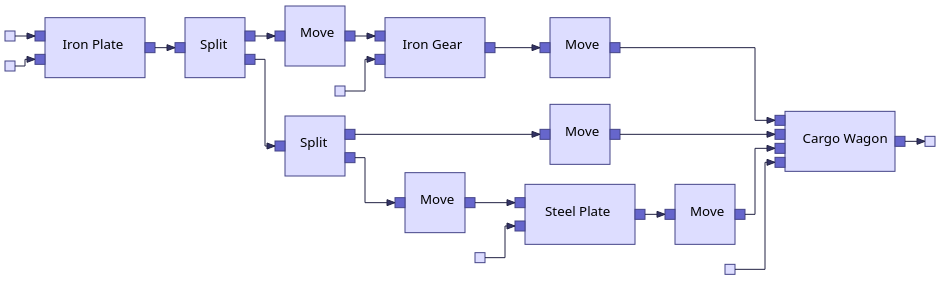
\includegraphics[width=\textwidth]{img/cargo_port_graph.png}
  \caption{
    Visualisation of a port graph constructed by our framework to represent a composition from a manufacturing domain (see Section~\ref{sec:cases/factorio} for a discussion of that domain).
    The composition has 11 primitive actions, represented here by nodes.
    Composition operations and resource actions yield the connections between ports of those nodes, representing resources.
  }
  \label{fig:cargo_port_graph}
\end{figure}

Our verification culminates in a graphical characterisation of composition linearity and its proof for every valid composition.
It serves as a counterpart to Chapter~\ref{ch:linearity}, where linearity is demonstrated by appealing to linear logic.
This characterisation of linearity specifies more directly which connections between actions are allowed.

At present, our approach is limited to sequential and parallel process compositions, because we find the base form of port graphs insufficient for expressing non-deterministic and higher-order features.
As a result, we do not provide a port graph mapping for optional composition, process representation or their associated resource actions (such as \isa{InjectL} and \isa{Apply}).
The most direct strand of future work, outlined in Section~\ref{sec:port_graphs/conc}, aims to extend port graphs and their mechanisation to cover such features and allow for a fully formal graphical representation of \emph{all} process compositions.

The remainder of this chapter proceeds as follows.
In Section~\ref{sec:port_graphs/rel} we highlight some related work on port graphs and then in Section~\ref{sec:port_graphs/pg} we introduce the notion of port graphs with a focus on the aspects relevant to our mechanisation.
In Section~\ref{sec:port_graphs/mech} we describe our mechanisation of port graphs in general, which forms a self-contained theory that can be reused for other applications.
Then in Section~\ref{sec:port_graphs/process} we give our mapping of process compositions to a specific kind of port graphs and discuss some of its basic properties.
In Section~\ref{sec:port_graphs/interchange} we use port graphs to prove when sequential and parallel process composition operations distribute over each other.
In Section~\ref{sec:port_graphs/linearity} we use port graphs to characterise process linearity in terms of allowed connections between actions, and prove it to hold for valid process compositions.
In Section~\ref{sec:port_graphs/trans} we define a transition system for port graphs, showing that equivalent port graphs have equivalent transitions.
This gives a behavioural dimension to equivalences between port graphs that we prove in prior sections.
Finally, in Section~\ref{sec:port_graphs/conc} we give concluding remarks and outline future work.

\section{Related Work}
\label{sec:port_graphs/rel}

Port graphs and port graph rewriting systems have been used to model various complex systems.
For instance, Andrei et al.~\cite{andrei_et_al-2011} use them to model biochemical processes and Vallet et al.~\cite{vallet_et_al-2015} use them to model social networks.
In comparison to ordinary graphs, the advantage of port graphs is that they allow us to model the specific points where edges connect to nodes.
This is useful to represent, for instance, protein sites in biochemistry or communication ports in computer networks.
In our case, they are crucial to representing specific input and output resources of individual actions.

Port graphs are also connected to graphical representations arising in applications of category theory.
In their book on applied category theory, Fong and Spivak~\cite{fong_spivak-2019} use port graphs in their formalisation of signal flow graphs, a graphical language used for instance in signal processing.
As shown for instance by Bonchi et al.~\cite{bonchi_et_al-2015}, signal flow graphs can be viewed as string diagrams, which are widely used in the study of monoidal categories~\cite{maclane-1998}.
Through monoidal categories, string diagrams connect to a wide range of graphical representations in applied category theory, such as the ZX calculus in the study of quantum circuits~\cite{coecke_duncan-2008,kissinger_zamdzhiev-2015}.
As such, there is evidence for the fruitful use of port graphs to formalise graphical representations.

Note that, in the literature, port graphs are often formalised with a set of nodes, a set of ports and a function from ports to nodes expressing to which node each port is attached.
In our mechanisation we diverge from this representation and instead formalise the ports attached to each node as part of that node.
This means that, in mechanising operations on port graphs, we are modifying collections instead of updating functions.
We find this approach to be easier to verify.
Nevertheless, we can recover the attachment function from our formalisation and, as such, we do not lose anything by using our approach.

Another use of port graphs is the Incredible Proof Machine~\cite{breitner_2016}, a tool for visual construction of proofs.
It uses port graphs to represent proofs, with nodes representing inference rules and ports their premises and conclusions.
Notably, the meta theory of this tool is verified in Isabelle/HOL~\cite{Incredible_Proof_Machine-AFP}.
As far as we are aware, this is the only published mechanisation of port graphs.
However, it is specific to their use as part of the tool being verified.
For instance, they do not support open ports, which we find vital to defining operations connecting multiple port graphs (see Section~\ref{sec:port_graphs/mech/seq}).
Instead of adapting this mechanisation, we choose to develop our own.

\section{Port Graphs}
\label{sec:port_graphs/pg}

Port graphs~\cite{andrei_2008} refine the notion of directed graphs.
Recall that the latter consist of a collection of nodes and a collection of edges going from one node to another.
(Undirected graphs simply discard the distinction between edge origin and destination.)

\begin{figure}[htbp]
  \centering
  \includesvg[scale=0.5]{img/pg_intro_0}
  \caption{Example directed graph with three nodes and three edges}
  \label{fig:pg_intro_0}
\end{figure}

As suggested by their name, port graphs modify directed graphs with \emph{ports} to mediate the connection between nodes and edges.
They are still formed by collections of nodes and edges, but every node has a collection of ports attached to it and edges go between ports instead of the nodes themselves.
Note that this does not require all ports to have an adjacent edge.
The ports allow us to express where and how nodes are connected, instead of simply saying that they are connected or not.

In practice, these ports have been used to express sites on proteins when representing biological processes~\cite{andrei_et_al-2011}, or input and output signals in signal flow graphs~\cite{fong_spivak-2019}.

\begin{figure}[htbp]
  \centering
  \includesvg[scale=0.5]{img/pg_intro_1}
  \caption{Example port graph with three nodes, three edges and eight ports, two of which are left unconnected}
  \label{fig:pg_intro_1}
\end{figure}

Note that it is possible to turn any port graph into a directed graph, essentially forgetting the connection details that the ports express.
We can do this by taking the same range of nodes as the port graph and then, for every edge of the port graph we ensure there is an edge in the directed graph that goes from the originating port's node to the destination port's node.
If the port graph edges express dependencies, as they do for our process port graphs, then the directed graph constructed in this way can be used to check for dependency loops.
We make use of this when discussing a transition system for port graphs in Section~\ref{sec:port_graphs/trans} to show when it terminates.
This graph is sometimes called the \emph{internal flow graph}~\cite{fong_spivak-2019}.

\emph{Labelled} port graphs~\cite{fernandez_et_al-2019} extend this idea further by labelling each node, port and edge with arbitrary data.
This is of great practical use when the port graph is used to represent additional information.
For instance, a representation of a distributed system may label nodes with IP addresses and ports with port numbers.

\begin{figure}[htbp]
  \centering
  \includesvg[scale=0.5,pretex=\relscale{0.8}\tt]{img/pg_intro_lab}
  \caption{Example port graph with simple text labels on nodes and ports}
  \label{fig:pg_intro_lab}
\end{figure}

In our case we use node and port labels for multiple purposes.
We name nodes based on the corresponding primitive action's position in the composition to uniquely identify them and we annotate them with its label and metadata.
We label ports with a combination of side (e.g.\ input and output for processes) and index to uniquely identify them in their collections and we annotate them with the resources they carry.

\emph{Open} port graphs address connecting port graphs to form larger ones.
They add a number of ports not attached to any node, which we may call \emph{open}, that are available for connection from some outside environment.
Then two port graphs may be combined by describing how their open ports are to be connected to form new edges.
\cbar{Note that having open ports not attached to any node allows us to have meaningful port graphs with no nodes.
These are useful when combining port graphs, for instance to reorder how existing edges connect to open ports or to disconnect some of them.}

\begin{figure}[htbp]
  \centering
  \includesvg[scale=0.5,pretex=\relscale{0.8}\tt]{img/pg_intro_open}
  \caption{Example labelled port graph with port \texttt{c2} connected to the open port \texttt{p}}
  \label{fig:pg_intro_open}
\end{figure}

This variant is useful when reasoning about port graphs in category theory, where it is vital to have a notion of interface (which here would be the collection of open ports) and composition~\cite{fong_spivak-2019}.

In our case, we use open ports for the input and output resources of the process being represented.
Sequential process composition then uses those open ports to form the relevant new connections.

\emph{Hierarchical} port graphs~\cite{ene_et_al-2018} allow for nodes to contain whole other port graphs within them.
As the name suggests, these are useful for going beyond connection and representing hierarchical structure as well.
This allows them to represent multi-layer systems as well as representing multiple layers of abstraction.

At present, we do not mechanise hierarchical port graphs or make use of them to represent process compositions.
However, their existence suggests a future extension to our mechanisation of port graphs that may improve the range of features they can express.
See Section~\ref{sec:port_graphs/conc} for our discussion of future work.

In the next section we describe our mechanisation of open port graphs with port and node labels.
We then use this theory in succeeding sections to graphically represent process compositions and verify properties about connections between individual actions.

\section{Mechanisation of Port Graphs}
\label{sec:port_graphs/mech}

We mechanise port graphs in two parts: their data and the constraints on that data.
We then define operations on the data and verify that they preserve those constraints (among other properties).

The data itself we represent using a datatype, which gathers the nodes, edges and open ports.
To make implementing operations on port graphs simpler, we use lists for all three collections to represent finite sets.

The constraints on the data we represent as locales, which are Isabelle's construct for collecting together assumptions and the facts stemming from them.
This means that if the data satisfies the locale assumptions, then the facts of the locale are true of the data.

The operations we define are ultimately in service of graphically representing process compositions.
However, we keep this part of the theory more general to make it reusable in other contexts.

\subsection{Ports}
\label{sec:port_graphs/mech/ports}

Before we state exactly how the data is represented, recall from Section~\ref{sec:proc/diag/paths} our definition of (qualified) ports (reproduced in Definition~\ref{isa:port+qualified}).
\cbar{We will now be using their general definitions to mechanise port graphs that allow for any port sides, labels and qualifying atoms.
In Section~\ref{sec:port_graphs/process/prelim} we then specialise these type variables in the same way we did for process diagrams in Section~\ref{sec:proc/diag/paths} to yield process port graphs.
That is, we will use input and output as port sides, resources as port labels and composition tree paths as atoms qualifying the ports.}

\begin{isadef}[Datatypes of ports and qualified ports]{isa:port+qualified}
  \isacomm{datatype}\isamarkupfalse%
\ {\isacharparenleft}\isatv{s}{\isacharcomma}\ \isatv{a}{\isacharparenright}\ port\ {\isacharequal}\ Port\ {\isacharparenleft}\isafv{side}{\isacharcolon}\ \isatv{s}{\isacharparenright}\ {\isacharparenleft}\isafv{index}{\isacharcolon}\ nat{\isacharparenright}\ {\isacharparenleft}\isafv{label}{\isacharcolon}\ \isatv{a}{\isacharparenright}

\item
  \isacomm{datatype}\isamarkupfalse%
\ {\isacharparenleft}\isatv{s}{\isacharcomma}\ \isatv{a}{\isacharcomma}\ \isatv{p}{\isacharparenright}\ qualified{\isacharunderscore}port\ {\isacharequal}\ QPort\ {\isacharparenleft}\isafv{port}{\isacharcolon}\ {\isachardoublequoteopen}{\isacharparenleft}\isatv{s}{\isacharcomma}\ \isatv{a}{\isacharparenright}\ port{\isachardoublequoteclose}{\isacharparenright}\ {\isacharparenleft}\isafv{name}{\isacharcolon}\ {\isachardoublequoteopen}\isatv{p}\ list{\isachardoublequoteclose}{\isacharparenright}

\end{isadef}

Note that names are sequences of atoms rather than simply an arbitrary type.
This allows us to further qualify an already qualified port with an additional atom.
When done to two collections of ports with two distinct atoms, this allows us to easily make those two collections disjoint.
For qualified ports, this operation is defined as follows:
\begin{isadef}[Further qualifying a qualified port]{isa:qualifyQPort}
  \isacomm{primrec}\isamarkupfalse%
\ qualifyQPort\ {\isacharcolon}{\isacharcolon}\ {\isachardoublequoteopen}\isatv{p}\ {\isasymRightarrow}\ {\isacharparenleft}\isatv{s}{\isacharcomma}\ \isatv{a}{\isacharcomma}\ \isatv{p}{\isacharparenright}\ qualified{\isacharunderscore}port\ {\isasymRightarrow}\ {\isacharparenleft}\isatv{s}{\isacharcomma}\ \isatv{a}{\isacharcomma}\ \isatv{p}{\isacharparenright}\ qualified{\isacharunderscore}port{\isachardoublequoteclose}\isanewline
\ \ \isaOcomm{where}\ {\isachardoublequoteopen}\isafv{qualifyQPort}\ \isabv{x}\ {\isacharparenleft}QPort\ \isabv{port\ path}{\isacharparenright}\ {\isacharequal}\ QPort\ \isabv{port}\ {\isacharparenleft}\isabv{x}\ {\isacharhash}\ \isabv{path}{\isacharparenright}{\isachardoublequoteclose}

\end{isadef}

\subsection{Nodes, Edges and Places}
\label{sec:port_graphs/mech/parts}

Nodes, edges and places are the different parts of port graphs.
While the first two represent exactly those basic graph components, places represent the union of both ports attached to nodes (which we call \emph{ground} ports) and open ports, which are not attached to a node.
In other words, places are what edges can connect.

Nodes are formed from a name (again a sequence of atoms drawn from type \isa{\isatv{p}}), a label drawn from type \isa{\isatv{l}} and the ports attached to the node (themselves drawing sides from type \isa{\isatv{s}} and labels from type \isa{\isatv{a}}).
Mechanised in Isabele/HOL:
\begin{isadef}[Datatype of nodes]{isa:node}
  \isacomm{datatype}\isamarkupfalse%
\ {\isacharparenleft}\isatv{s}{\isacharcomma}\ \isatv{a}{\isacharcomma}\ \isatv{p}{\isacharcomma}\ \isatv{l}{\isacharparenright}\ node\ {\isacharequal}\isanewline
\ \ Node\ {\isacharparenleft}\isafv{node{\isacharunderscore}name}{\isacharcolon}\ {\isachardoublequoteopen}\isatv{p}\ list{\isachardoublequoteclose}{\isacharparenright}\ {\isacharparenleft}\isafv{node{\isacharunderscore}label}{\isacharcolon}\ \isatv{l}{\isacharparenright}\ {\isacharparenleft}\isafv{node{\isacharunderscore}ports}{\isacharcolon}\ {\isachardoublequoteopen}{\isacharparenleft}\isatv{s}{\isacharcomma}\ \isatv{a}{\isacharparenright}\ port\ list{\isachardoublequoteclose}{\isacharparenright}

\end{isadef}
Note that in Section~\ref{sec:port_graphs/process/prelim}, when specifying port graphs for process compositions, we instantiate the node labels to carry the labels and metadata of primitive actions.

Places can be either ground ports, qualified by a node name, or open ports.
We mechanise them in Isabelle/HOL as follows (with type variables \isatv{s}, \isatv{a} and \isatv{p} again just as with qualified ports):
\begin{isadef}[Datatype of places]{isa:place}
  \isacomm{datatype}\isamarkupfalse%
\ {\isacharparenleft}\isatv{s}{\isacharcomma}\ \isatv{a}{\isacharcomma}\ \isatv{p}{\isacharparenright}\ place\ {\isacharequal}\isanewline
\ \ \ \ place{\isacharunderscore}ground{\isacharcolon}\ GroundPort\ \isapars{{\isachardoublequoteopen}{\isacharparenleft}\isatv{s}{\isacharcomma}\ \isatv{a}{\isacharcomma}\ \isatv{p}{\isacharparenright}\ qualified{\isacharunderscore}port{\isachardoublequoteclose}}\isanewline
\ \ {\isacharbar}\ place{\isacharunderscore}open{\isacharcolon}\ OpenPort\ \isapars{{\isachardoublequoteopen}{\isacharparenleft}\isatv{s}{\isacharcomma}\ \isatv{a}{\isacharparenright}\ port{\isachardoublequoteclose}}

\end{isadef}
The automatically generated predicates \isa{place{\isacharunderscore}ground} and \isa{place{\isacharunderscore}open} allow us to easily distinguish the two kinds of places, which is a frequent point in proofs.

With both nodes and places defined, we can for instance define how all the ground places induced by a node can be collected:
\begin{isadef}[Collecting ground places of a node]{isa:nodePlaces}
  \isacomm{fun}\isamarkupfalse%
\ nodePlaces\ {\isacharcolon}{\isacharcolon}\ {\isachardoublequoteopen}{\isacharparenleft}\isatv{s}{\isacharcomma}\ \isatv{a}{\isacharcomma}\ \isatv{p}{\isacharcomma}\ \isatv{l}{\isacharparenright}\ node\ {\isasymRightarrow}\ {\isacharparenleft}\isatv{s}{\isacharcomma}\ \isatv{a}{\isacharcomma}\ \isatv{p}{\isacharparenright}\ place\ list{\isachardoublequoteclose}\isanewline
\ \ \isaOcomm{where}\ {\isachardoublequoteopen}\isafv{nodePlaces}\ \isabv{n}\ {\isacharequal}\isanewline
\ \ \ \ map\ {\isacharparenleft}{\isasymlambda}\isabv{p}{\isachardot}\ GroundPort\ {\isacharparenleft}QPort\ \isabv{p}\ {\isacharparenleft}node{\isacharunderscore}name\ \isabv{n}{\isacharparenright}{\isacharparenright}{\isacharparenright}\ {\isacharparenleft}node{\isacharunderscore}ports\ \isabv{n}{\isacharparenright}{\isachardoublequoteclose}%

\end{isadef}

Edges are made up of two places, the origin and destination, meaning they are simple and directed edges.
Mechanised in Isabelle/HOL (with type variables \isatv{s}, \isatv{a} and \isatv{p} again just as with qualified ports):
\begin{isadef}[Datatype of edges]{isa:edge}
  \isacomm{datatype}\isamarkupfalse%
\ {\isacharparenleft}\isatv{s}{\isacharcomma}\ \isatv{a}{\isacharcomma}\ \isatv{p}{\isacharparenright}\ edge\ {\isacharequal}\isanewline
\ \ Edge\ {\isacharparenleft}\isafv{edge{\isacharunderscore}from}{\isacharcolon}\ {\isachardoublequoteopen}{\isacharparenleft}\isatv{s}{\isacharcomma}\ \isatv{a}{\isacharcomma}\ \isatv{p}{\isacharparenright}\ place{\isachardoublequoteclose}{\isacharparenright}\ {\isacharparenleft}\isafv{edge{\isacharunderscore}to}{\isacharcolon}\ {\isachardoublequoteopen}{\isacharparenleft}\isatv{s}{\isacharcomma}\ \isatv{a}{\isacharcomma}\ \isatv{p}{\isacharparenright}\ place{\isachardoublequoteclose}{\isacharparenright}

\end{isadef}

We now illustrate these constructs before using them in port graphs.
\cbstart
Consider the \isa{add{\isacharunderscore}to{\isacharunderscore}credit} action from Definition~\ref{isa:add_to_credit}, say with existing credit of zero and adding ten in cash.
This action has two input atoms (\isa{Machine\ 0} and \isa{Cash\ 10}) and one output atom (\isa{Machine\ 10}).
Let this action be found as the first child under two sequential compositions, such as in the example in Section~\ref{sec:proc/type/res}.
While our full process port graph construction uses more complex labels (described in Section~\ref{sec:port_graphs/process}), we could represent this action with the node:
\begin{center}
  \begin{minipage}{0.75\textwidth}
    \begin{isabelle}
      Node\ \isalist{SeqL,\ SeqL}\isanewline
      \isaindent{Node\ }\isaString{Add\ to\ credit}\isanewline
      \isaindent{Node\ }\isalist{Port\ In\ \isadigit{0}\ \isapars{Res\ \isapars{Machine\ 0}},\ Port\ In\ \isadigit{1}\ \isapars{Res\ \isapars{Cash\ 10}},\isanewline
      \isaindent{Node\ {\isacharbrackleft}}Port\ Out\ \isadigit{0}\ \isapars{Res\ \isapars{Machine\ 10}}}
    \end{isabelle}
  \end{minipage}
\end{center}
and one of its places would then be:
\begin{isabelle}
\centering
  GroundPort\ \isapars{QPort\ \isapars{Port\ In\ \isadigit{0}\ \isapars{Res\ \isapars{Machine\ 0}}}\ \isalist{SeqL,\ SeqL}}
\end{isabelle}
Then, if this node was within a larger port graph that has the following open input port:
\begin{isabelle}
\centering
  Port\ In\ \isadigit{3}\ \isapars{Res\ \isapars{Machine\ 0}}
\end{isabelle}
we could connect this open port to the node's input with the following edge:
\begin{isabelle}
\centering
  Edge\ \widthtoR{\isapars{OpenPort\ \isapars{Port\ In\ \isadigit{3}\ \isapars{Res\ \isapars{Machine\ 0}}}}}{\isapars{GroundPort\ \isapars{QPort\ \isapars{Port\ In\ \isadigit{0}\ \isapars{Res\ \isapars{Machine\ 0}}}\ \isalist{SeqL,\ SeqL}}}}\isanewline
  \isaindent{Edge\ }\isapars{GroundPort\ \isapars{QPort\ \isapars{Port\ In\ \isadigit{0}\ \isapars{Res\ \isapars{Machine\ 0}}}\ \isalist{SeqL,\ SeqL}}}
\end{isabelle}
\cbend

\subsection{Port Graph Data}
\label{sec:port_graphs/mech/data}

With all the constituent parts defined, we can now mechanise the port graph data itself, with sides drawn from type \isa{\isatv{s}}, port labels drawn from type \isa{\isatv{a}}, name atoms drawn from type \isa{\isatv{p}} and node labels drawn from type \isa{\isatv{l}}:
\begin{isadef}[Datatype of port graphs]{isa:type-port_graph}
  \isacomm{datatype}\isamarkupfalse%
\ {\isacharparenleft}\isatv{s}{\isacharcomma}\ \isatv{a}{\isacharcomma}\ \isatv{p}{\isacharcomma}\ \isatv{l}{\isacharparenright}\ port{\isacharunderscore}graph\ {\isacharequal}\isanewline
\ \ PGraph\ {\isacharparenleft}\isafv{pg{\isacharunderscore}nodes}{\isacharcolon}\ {\isachardoublequoteopen}{\isacharparenleft}\isatv{s}{\isacharcomma}\ \isatv{a}{\isacharcomma}\ \isatv{p}{\isacharcomma}\ \isatv{l}{\isacharparenright}\ node\ list{\isachardoublequoteclose}{\isacharparenright}\isanewline
\isaindent{\ \ PGraph\ }{\isacharparenleft}\isafv{pg{\isacharunderscore}edges}{\isacharcolon}\ {\isachardoublequoteopen}{\isacharparenleft}\isatv{s}{\isacharcomma}\ \isatv{a}{\isacharcomma}\ \isatv{p}{\isacharparenright}\ edge\ list{\isachardoublequoteclose}{\isacharparenright}\isanewline
\isaindent{\ \ PGraph\ }{\isacharparenleft}\isafv{pg{\isacharunderscore}ports}{\isacharcolon}\ {\isachardoublequoteopen}{\isacharparenleft}\isatv{s}{\isacharcomma}\ \isatv{a}{\isacharparenright}\ port\ list{\isachardoublequoteclose}{\isacharparenright}%

\end{isadef}

On this data alone we make several useful definitions: a function to qualify the whole port graph, a function to collect all places occurring in it and a relation for port graphs with no names in common.

The function \isa{qualifyPortGraph} takes a name atom and prefixes it to names of all nodes in the port graph as well as the names qualifying ground places in edges.
We define it using a series of functions with the same effect on different targets, called \isa{qualifyNode}, \isa{qualifyEdge} and \isa{qualifyPlace}, culminating in \isa{qualifyPortGraph}.
All of these either qualify their target's constituent parts or, in the case of \isa{qualifyNode}, prefix its name with the atom just as \isa{qualifyQPort} in Section~\ref{sec:port_graphs/mech/ports} does.

The function \isa{pgraphPlaces} collects all the places occurring in the port graph by combining those attached to its nodes with its open ports.
This function figures frequently in proofs about port graphs and is defined as follows:
\pagebreak
\begin{isadef}[Collecting open and ground places of a port graph]{isa:pgraphPlaces}
  \isacomm{fun}\isamarkupfalse%
\ pgraphPlaces\ {\isacharcolon}{\isacharcolon}\ {\isachardoublequoteopen}{\isacharparenleft}\isatv{s}{\isacharcomma}\ \isatv{a}{\isacharcomma}\ \isatv{p}{\isacharcomma}\ \isatv{l}{\isacharparenright}\ port{\isacharunderscore}graph\ {\isasymRightarrow}\ {\isacharparenleft}\isatv{s}{\isacharcomma}\ \isatv{a}{\isacharcomma}\ \isatv{p}{\isacharparenright}\ place\ list{\isachardoublequoteclose}\isanewline
\ \ \isaOcomm{where}\ {\isachardoublequoteopen}\isafv{pgraphPlaces}\ \isabv{x}\ {\isacharequal}\isanewline
\ \ \ \ concat\ {\isacharparenleft}map\ nodePlaces\ {\isacharparenleft}pg{\isacharunderscore}nodes\ \isabv{x}{\isacharparenright}{\isacharparenright}\ {\isacharat}\isanewline
\ \ \ \ map\ OpenPort\ {\isacharparenleft}pg{\isacharunderscore}ports\ \isabv{x}{\isacharparenright}{\isachardoublequoteclose}%

\end{isadef}

Being able to tell that two port graphs do not have a name in common is useful because such a shared name would interfere when combining them.
While this makes a frequent assumption in our verification, it is easy to satisfy by using \isa{qualifyPortGraph} to qualify all names within each port graph with one of two distinct name atoms.
We call port graphs satisfying this relation \emph{disjoint} and define it in Isabelle/HOL as follows:
\begin{isadef}[Disjoint port graphs]{isa:pg_disjoint}
  \isacomm{definition}\isamarkupfalse%
\ pg{\isacharunderscore}disjoint\ {\isacharcolon}{\isacharcolon}\ {\isachardoublequoteopen}{\isacharparenleft}\isatv{s}{\isacharcomma}\ \isatv{a}{\isacharcomma}\ \isatv{p}{\isacharcomma}\ \isatv{l}{\isacharparenright}\ port{\isacharunderscore}graph\ {\isasymRightarrow}\ {\isacharparenleft}\isatv{s}{\isacharcomma}\ \isatv{a}{\isacharcomma}\ \isatv{p}{\isacharcomma}\ \isatv{l}{\isacharparenright}\ port{\isacharunderscore}graph\ {\isasymRightarrow}\ bool{\isachardoublequoteclose}\isanewline
\ \ \isaOcomm{where}\ {\isachardoublequoteopen}\isafv{pg{\isacharunderscore}disjoint}\ \isabv{x\ y}\ {\isacharequal}\isanewline
\ \ \ \ {\isacharparenleft}{\isasymforall}\isabv{m\ n}{\isachardot}\ \isabv{m}\ {\isasymin}\ set\ {\isacharparenleft}pg{\isacharunderscore}nodes\ \isabv{x}{\isacharparenright}\ {\isasymand}\ \isabv{n}\ {\isasymin}\ set\ {\isacharparenleft}pg{\isacharunderscore}nodes\ \isabv{y}{\isacharparenright}\isanewline
\isaindent{\ \ \ \ {\isacharparenleft}{\isasymforall}\isabv{m\ n}{\isachardot}\ }{\isasymlongrightarrow}\ node{\isacharunderscore}name\ \isabv{m}\ {\isasymnoteq}\ node{\isacharunderscore}name\ \isabv{n}{\isacharparenright}{\isachardoublequoteclose}

\end{isadef}

\subsection{Well-Formed Port Graphs}
\label{sec:port_graphs/mech/base_locale}

While we can now express the data of a port graph, nothing guarantees that it is sensible.
We could for instance include an edge between places that are not in the port graph, or two nodes with the same name.

To address this, we make a number of requirements of the port graph data in order to call it an actual port graph, which we collect into the locale \isa{port{\isacharunderscore}graph} shown in Definition~\ref{isa:locale-port_graph}.
A locale acts as a predicate, but with more convenient automation in proofs.
We list the requirements next, with a brief motivation in each case:
\begin{description}[style=nextline]
  \item[\isa{edge{\isacharunderscore}from{\isacharunderscore}pg} and \isa{edge{\isacharunderscore}to{\isacharunderscore}pg}]
    Origin and destination of every edge in the port graph must be places of that port graph.
  \item[\isa{node{\isacharunderscore}unique{\isacharunderscore}name}]
    No two nodes of the port graph can have the same name, so we can use the name to identify a node.
  \item[\isa{ports{\isacharunderscore}index{\isacharunderscore}bound}]
    Index of every open port of the port graph is less than the total number of open ports on the same side.
  \item[\isa{open{\isacharunderscore}ports{\isacharunderscore}label{\isacharunderscore}eq}]
    Any two open ports of the port graph that have the same side and index must also have the same label, and thus be the same port.
  \item[\isa{node{\isacharunderscore}ports{\isacharunderscore}label{\isacharunderscore}eq}]
    Any two ports of a node of the port graph that have the same side and index must also have the same label, and thus be the same port.
  \item[\isa{nodes{\isacharunderscore}distinct}, \isa{edges{\isacharunderscore}distinct} and \isa{ports{\isacharunderscore}distinct}]
    Node, edge and open port lists do not contain duplicates, so that they represent finite sets.
\end{description}

\begin{isadef}[Well-formed port graphs]{isa:locale-port_graph}
  \isacomm{locale}\isamarkupfalse%
\ port{\isacharunderscore}graph\ {\isacharequal}\isanewline
\ \ \ \ \ \ \ \ \isaOcomm{fixes}\ \isafv{G}\ {\isacharcolon}{\isacharcolon}\ {\isachardoublequoteopen}{\isacharparenleft}\isatv{s}{\isacharcomma}\ \isatv{a}{\isacharcomma}\ \isatv{p}{\isacharcomma}\ \isatv{l}{\isacharparenright}\ port{\isacharunderscore}graph{\isachardoublequoteclose}\isanewline
\ \ \isaOcomm{assumes}\ edge{\isacharunderscore}from{\isacharunderscore}pg{\isacharcolon}\isanewline
\ \ \ \ {\isachardoublequoteopen}{\isasymAnd}\isabv{e}{\isachardot}\ \isabv{e}\ {\isasymin}\ set\ {\isacharparenleft}pg{\isacharunderscore}edges\ \isafv{G}{\isacharparenright}\ {\isasymLongrightarrow}\ edge{\isacharunderscore}from\ \isabv{e}\ {\isasymin}\ set\ {\isacharparenleft}pgraphPlaces\ \isafv{G}{\isacharparenright}{\isachardoublequoteclose}\isanewline
\ \ \ \ \ \ \ \ \ \ \isaOcomm{and}\ edge{\isacharunderscore}to{\isacharunderscore}pg{\isacharcolon}\isanewline
\ \ \ \ {\isachardoublequoteopen}{\isasymAnd}\isabv{e}{\isachardot}\ \isabv{e}\ {\isasymin}\ set\ {\isacharparenleft}pg{\isacharunderscore}edges\ \isafv{G}{\isacharparenright}\ {\isasymLongrightarrow}\ edge{\isacharunderscore}to\ \isabv{e}\ {\isasymin}\ set\ {\isacharparenleft}pgraphPlaces\ \isafv{G}{\isacharparenright}{\isachardoublequoteclose}\isanewline
\ \ \ \ \ \ \ \ \ \ \isaOcomm{and}\ node{\isacharunderscore}unique{\isacharunderscore}name{\isacharcolon}\isanewline
\ \ \ \ {\isachardoublequoteopen}{\isasymAnd}\isabv{m\ n}{\isachardot}\ {\isasymlbrakk}\isabv{m}\ {\isasymin}\ set\ {\isacharparenleft}pg{\isacharunderscore}nodes\ \isafv{G}{\isacharparenright}{\isacharsemicolon}\ \isabv{n}\ {\isasymin}\ set\ {\isacharparenleft}pg{\isacharunderscore}nodes\ \isafv{G}{\isacharparenright}{\isacharsemicolon}\ node{\isacharunderscore}name\ \isabv{m}\ {\isacharequal}\ node{\isacharunderscore}name\ \isabv{n}{\isasymrbrakk}\isanewline
\isaindent{\ \ \ \ {\isachardoublequoteopen}{\isasymAnd}m\ n{\isachardot}\ }{\isasymLongrightarrow}\ \isabv{m}\ {\isacharequal}\ \isabv{n}{\isachardoublequoteclose}\isanewline
\ \ \ \ \ \ \ \ \ \ \isaOcomm{and}\ ports{\isacharunderscore}index{\isacharunderscore}bound{\isacharcolon}\isanewline
\ \ \ \ {\isachardoublequoteopen}{\isasymAnd}\isabv{p}{\isachardot}\ \isabv{p}\ {\isasymin}\ set\ {\isacharparenleft}pg{\isacharunderscore}ports\ \isafv{G}{\isacharparenright}\isanewline
\isaindent{\ \ \ \ {\isachardoublequoteopen}{\isasymAnd}p{\isachardot}\ }{\isasymLongrightarrow}\ port{\isachardot}index\ \isabv{p}\ {\isacharless}\ length\ {\isacharparenleft}filter\ {\isacharparenleft}{\isasymlambda}\isabv{x}{\isachardot}\ port{\isachardot}side\ \isabv{x}\ {\isacharequal}\ port{\isachardot}side\ \isabv{p}{\isacharparenright}\ {\isacharparenleft}pg{\isacharunderscore}ports\ \isafv{G}{\isacharparenright}{\isacharparenright}{\isachardoublequoteclose}\isanewline
\ \ \ \ \ \ \ \ \ \ \isaOcomm{and}\ open{\isacharunderscore}ports{\isacharunderscore}label{\isacharunderscore}eq{\isacharcolon}\isanewline
\ \ \ \ {\isachardoublequoteopen}{\isasymAnd}\isabv{p\ q}{\isachardot}\ {\isasymlbrakk}\isabv{p}\ {\isasymin}\ set\ {\isacharparenleft}pg{\isacharunderscore}ports\ \isafv{G}{\isacharparenright}{\isacharsemicolon}\ \isabv{q}\ {\isasymin}\ set\ {\isacharparenleft}pg{\isacharunderscore}ports\ \isafv{G}{\isacharparenright}{\isacharsemicolon}\isanewline
\isaindent{\ \ \ \ {\isachardoublequoteopen}{\isasymAnd}p\ q{\isachardot}\ {\isasymlbrakk}}port{\isachardot}side\ \isabv{p}\ {\isacharequal}\ port{\isachardot}side\ \isabv{q}{\isacharsemicolon}\ port{\isachardot}index\ \isabv{p}\ {\isacharequal}\ port{\isachardot}index\ \isabv{q}{\isasymrbrakk}\isanewline
\isaindent{\ \ \ \ {\isachardoublequoteopen}{\isasymAnd}p\ q{\isachardot}\ }{\isasymLongrightarrow}\ port{\isachardot}label\ \isabv{p}\ {\isacharequal}\ port{\isachardot}label\ \isabv{q}{\isachardoublequoteclose}\isanewline
\ \ \ \ \ \ \ \ \ \ \isaOcomm{and}\ node{\isacharunderscore}ports{\isacharunderscore}label{\isacharunderscore}eq{\isacharcolon}\isanewline
\ \ \ \ {\isachardoublequoteopen}{\isasymAnd}\isabv{n\ p\ q}{\isachardot}\ {\isasymlbrakk}\isabv{n}\ {\isasymin}\ set\ {\isacharparenleft}pg{\isacharunderscore}nodes\ \isafv{G}{\isacharparenright}{\isacharsemicolon}\ \isabv{p}\ {\isasymin}\ set\ {\isacharparenleft}node{\isacharunderscore}ports\ \isabv{n}{\isacharparenright}{\isacharsemicolon}\ \isabv{q}\ {\isasymin}\ set\ {\isacharparenleft}node{\isacharunderscore}ports\ \isabv{n}{\isacharparenright}{\isacharsemicolon}\isanewline
\isaindent{\ \ \ \ {\isachardoublequoteopen}{\isasymAnd}\isabv{n\ p\ q}{\isachardot}\ {\isasymlbrakk}}port{\isachardot}side\ \isabv{p}\ {\isacharequal}\ port{\isachardot}side\ \isabv{q}{\isacharsemicolon}\ port{\isachardot}index\ \isabv{p}\ {\isacharequal}\ port{\isachardot}index\ \isabv{q}{\isasymrbrakk}\isanewline
\isaindent{\ \ \ \ {\isachardoublequoteopen}{\isasymAnd}\isabv{n\ p\ q}{\isachardot}\ }{\isasymLongrightarrow}\ port{\isachardot}label\ \isabv{p}\ {\isacharequal}\ port{\isachardot}label\ \isabv{q}{\isachardoublequoteclose}\isanewline
\ \ \ \ \ \ \ \ \ \ \isaOcomm{and}\ nodes{\isacharunderscore}distinct{\isacharcolon}\ {\isachardoublequoteopen}distinct\ {\isacharparenleft}pg{\isacharunderscore}nodes\ \isafv{G}{\isacharparenright}{\isachardoublequoteclose}\isanewline
\ \ \ \ \ \ \ \ \ \ \isaOcomm{and}\ edges{\isacharunderscore}distinct{\isacharcolon}\ {\isachardoublequoteopen}distinct\ {\isacharparenleft}pg{\isacharunderscore}edges\ \isafv{G}{\isacharparenright}{\isachardoublequoteclose}\isanewline
\ \ \ \ \ \ \ \ \ \ \isaOcomm{and}\ ports{\isacharunderscore}distinct{\isacharcolon}\ {\isachardoublequoteopen}distinct\ {\isacharparenleft}pg{\isacharunderscore}ports\ \isafv{G}{\isacharparenright}{\isachardoublequoteclose}

\end{isadef}

One implication of this locale is that we can define a function that given a ground port retrieves the node in the port graph it is attached to.
The good behaviour of this function relies on assumptions of the locale for both the existence and uniqueness of the node.
As noted in Section~\ref{sec:port_graphs/rel}, some formulations of port graphs in the literature start with such a function instead of making ports part of the node data as we do.
We can recover this function from data satisfying our assumptions.

\subsection{Port Graph With Flow}
\label{sec:port_graphs/mech/flow_locale}

Beyond the basic requirements, the port graphs used to represent process compositions are even more specific.
They have two special sides, input and output, and the direction of edges represents the flow of resources between actions.
As such, they should not contain, for instance, edges going into an output port of an action, because that is not a place that can receive a resource.
We characterise this through the following extra requirements on well-formed port graphs:
\begin{itemize}
  \item The possible sides include two specially designated ones, input and output, and
  \item All edges that touch some input or output place have both:
    \begin{itemize}
      \item Origin in an open input port or ground output port, and
      \item Destination in an open output port or ground input port.
    \end{itemize}
\end{itemize}

When mechanising these assumptions in Isabelle/HOL we first define a simple type class to generically capture the two designated sides.
Type classes~\cite{wenzel-1997} are a variant of locales constrained to a single type variable, letting us define constants and assumptions about them, that act as constraints on types.
They allow us to sort types and safely overload definitions.
In order to use the class constants with a type, we need to show that this type is an instance of the class by proving that it satisfies all assumptions of the class.

Here we use a type class to define convenient syntax for the input and output sides (\isa{In} and \isa{Out}) and capture the implicit assumption that they are distinct.
This lets us later instantiate those elements as we please, see for instance Section~\ref{sec:port_graphs/process/prelim}.
\begin{isadef}[Typeclass capturing distinct input and output sides]{isa:side_in_out}
  \isacomm{class}\isamarkupfalse%
\ side{\isacharunderscore}in{\isacharunderscore}out\ {\isacharequal}\isanewline
\ \ \ \ \ \ \ \ \isaOcomm{fixes}\ \isafv{In}\ {\isacharcolon}{\isacharcolon}\ \isatv{a}\ \isaOcomm{and}\ \isafv{Out}\ {\isacharcolon}{\isacharcolon}\ \isatv{a}\isanewline
\ \ \isaOcomm{assumes}\ in{\isacharunderscore}out{\isacharunderscore}distinct{\isacharcolon}\ {\isachardoublequoteopen}\isafv{In}\ {\isasymnoteq}\ \isafv{Out}{\isachardoublequoteclose}

\end{isadef}

We then abbreviate the precondition on edges, with \isa{edge{\isacharunderscore}in{\isacharunderscore}flow\ \isafv{e}} meaning that \isa{\isafv{e}} has either origin or destination with side \isa{In} or \isa{Out}:
\begin{isadef}[Flow precondition on edges]{isa:edge_in_flow}
  \isacomm{definition}\ edge{\isacharunderscore}in{\isacharunderscore}flow\ {\isacharcolon}{\isacharcolon}\ {\isachardoublequoteopen}{\isacharparenleft}\isatv{s}\ {\isacharcolon}{\isacharcolon}\ side{\isacharunderscore}in{\isacharunderscore}out{\isacharcomma}\ \isatv{a}{\isacharcomma}\ \isatv{p}{\isacharparenright}\ edge\ {\isasymRightarrow}\ bool{\isachardoublequoteclose}\isanewline
\ \ \isaOcomm{where}\ {\isachardoublequoteopen}\isafv{edge{\isacharunderscore}in{\isacharunderscore}flow}\ \isabv{e}\ {\isacharequal}\ {\isacharparenleft}place{\isacharunderscore}side\ {\isacharparenleft}edge{\isacharunderscore}from\ \isabv{e}{\isacharparenright}\ {\isasymin}\ {\isacharbraceleft}In{\isacharcomma}\ Out{\isacharbraceright}\ {\isasymor}\isanewline
\isaindent{\ \ \isaOcomm{where}\ {\isachardoublequoteopen}\isafv{edge{\isacharunderscore}in{\isacharunderscore}flow}\ \isabv{e}\ {\isacharequal}\ {\isacharparenleft}}place{\isacharunderscore}side\ {\isacharparenleft}edge{\isacharunderscore}to\ \isabv{e}{\isacharparenright}\ {\isasymin}\ {\isacharbraceleft}In{\isacharcomma}\ Out{\isacharbraceright}{\isacharparenright}{\isachardoublequoteclose}

\end{isadef}
\noindent
and with it we mechanise the full assumptions as the locale \isa{port{\isacharunderscore}graph{\isacharunderscore}flow}:
\begin{isadef}[Port graphs with flow]{isa:port_graph_flow}
  \isacomm{locale}\isamarkupfalse%
\ port{\isacharunderscore}graph{\isacharunderscore}flow\ {\isacharequal}\isanewline
\ \ port{\isacharunderscore}graph\ \isafv{G}\ \isaOcomm{for}\ \isafv{G}\ {\isacharcolon}{\isacharcolon}\ {\isachardoublequoteopen}{\isacharparenleft}\isatv{s}\ {\isacharcolon}{\isacharcolon}\ side{\isacharunderscore}in{\isacharunderscore}out{\isacharcomma}\ \isatv{a}{\isacharcomma}\ \isatv{p}{\isacharcomma}\ \isatv{l}{\isacharparenright}\ port{\isacharunderscore}graph{\isachardoublequoteclose}\ {\isacharplus}\isanewline
\ \ \isaOcomm{assumes}\ edge{\isacharunderscore}from{\isacharunderscore}open{\isacharcolon}\isanewline
\ \ \ \ {\isachardoublequoteopen}{\isasymlbrakk}\isabv{e}\ {\isasymin}\ set\ {\isacharparenleft}pg{\isacharunderscore}edges\ \isafv{G}{\isacharparenright}{\isacharsemicolon}\ place{\isacharunderscore}open\ {\isacharparenleft}edge{\isacharunderscore}from\ \isabv{e}{\isacharparenright}{\isacharsemicolon}\ edge{\isacharunderscore}in{\isacharunderscore}flow\ \isabv{e}{\isasymrbrakk}\isanewline
\ \ \ \ \ \ {\isasymLongrightarrow}\ place{\isacharunderscore}side\ {\isacharparenleft}edge{\isacharunderscore}from\ \isabv{e}{\isacharparenright}\ {\isacharequal}\ In{\isachardoublequoteclose}\isanewline
\ \ \ \ \ \ \ \ \ \ \isaOcomm{and}\ edge{\isacharunderscore}to{\isacharunderscore}open{\isacharcolon}\isanewline
\ \ \ \ {\isachardoublequoteopen}{\isasymlbrakk}\isabv{e}\ {\isasymin}\ set\ {\isacharparenleft}pg{\isacharunderscore}edges\ \isafv{G}{\isacharparenright}{\isacharsemicolon}\ place{\isacharunderscore}open\ {\isacharparenleft}edge{\isacharunderscore}to\ \isabv{e}{\isacharparenright}{\isacharsemicolon}\ edge{\isacharunderscore}in{\isacharunderscore}flow\ \isabv{e}{\isasymrbrakk}\isanewline
\ \ \ \ \ \ {\isasymLongrightarrow}\ place{\isacharunderscore}side\ {\isacharparenleft}edge{\isacharunderscore}to\ \isabv{e}{\isacharparenright}\ {\isacharequal}\ Out{\isachardoublequoteclose}\isanewline
\ \ \ \ \ \ \ \ \ \ \isaOcomm{and}\ edge{\isacharunderscore}from{\isacharunderscore}ground{\isacharcolon}\isanewline
\ \ \ \ {\isachardoublequoteopen}{\isasymlbrakk}\isabv{e}\ {\isasymin}\ set\ {\isacharparenleft}pg{\isacharunderscore}edges\ \isafv{G}{\isacharparenright}{\isacharsemicolon}\ place{\isacharunderscore}ground\ {\isacharparenleft}edge{\isacharunderscore}from\ \isabv{e}{\isacharparenright}{\isacharsemicolon}\ edge{\isacharunderscore}in{\isacharunderscore}flow\ \isabv{e}{\isasymrbrakk}\isanewline
\ \ \ \ \ \ {\isasymLongrightarrow}\ place{\isacharunderscore}side\ {\isacharparenleft}edge{\isacharunderscore}from\ \isabv{e}{\isacharparenright}\ {\isacharequal}\ Out{\isachardoublequoteclose}\isanewline
\ \ \ \ \ \ \ \ \ \ \isaOcomm{and}\ edge{\isacharunderscore}to{\isacharunderscore}ground{\isacharcolon}\isanewline
\ \ \ \ {\isachardoublequoteopen}{\isasymlbrakk}\isabv{e}\ {\isasymin}\ set\ {\isacharparenleft}pg{\isacharunderscore}edges\ \isafv{G}{\isacharparenright}{\isacharsemicolon}\ place{\isacharunderscore}ground\ {\isacharparenleft}edge{\isacharunderscore}to\ \isabv{e}{\isacharparenright}{\isacharsemicolon}\ edge{\isacharunderscore}in{\isacharunderscore}flow\ \isabv{e}{\isasymrbrakk}\isanewline
\ \ \ \ \ \ {\isasymLongrightarrow}\ place{\isacharunderscore}side\ {\isacharparenleft}edge{\isacharunderscore}to\ \isabv{e}{\isacharparenright}\ {\isacharequal}\ In{\isachardoublequoteclose}

\end{isadef}

\subsection{Equivalence of Port Graphs}
\label{sec:port_graphs/mech/equiv}

Our formalisation of port graphs uses names to identify nodes, and it represents the collections of nodes, edges and ports with lists.
This means that two port graphs could differ in nothing but names assigned to one node, or in the order of elements in the lists, and be considered entirely distinct.
But we would like to draw a connection between such almost-identical port graphs.

We formalise this connection as an equivalence relation between port graphs, which we denote as \isa{\isasymapprox}.
For two port graphs to be equivalent we require that either both are ill-formed (i.e.\ do not satisfy the \isa{port{\isacharunderscore}graph} locale) or they are both well-formed, have the same set of open ports and it is possible to systematically rename nodes of each to give the nodes of the other in an invertible way.

\begin{isadef}[Witnesses of port graph equivalence]{isa:pgEquiv_witness}
  \isacomm{definition}\ pgEquiv{\isacharunderscore}witness\ {\isacharcolon}{\isacharcolon}\ {\isachardoublequoteopen}{\isacharparenleft}\isatv{p}\ list\ {\isasymRightarrow}\ \isatv{p}\ list{\isacharparenright}\ {\isasymRightarrow}\ {\isacharparenleft}\isatv{p}\ list\ {\isasymRightarrow}\ \isatv{p}\ list{\isacharparenright}\isanewline
\isaindent{\isacomm{definition}\ pgEquiv{\isacharunderscore}witness\ }{\isasymRightarrow}\ {\isacharparenleft}\isatv{s}{\isacharcomma}\ \isatv{a}{\isacharcomma}\ \isatv{p}{\isacharcomma}\ \isatv{l}{\isacharparenright}\ port{\isacharunderscore}graph\ {\isasymRightarrow}\ {\isacharparenleft}\isatv{s}{\isacharcomma}\ \isatv{a}{\isacharcomma}\ \isatv{p}{\isacharcomma}\ \isatv{l}{\isacharparenright}\ port{\isacharunderscore}graph\isanewline
\isaindent{\isacomm{definition}\ pgEquiv{\isacharunderscore}witness\ }{\isasymRightarrow}\ bool{\isachardoublequoteclose}\isanewline
\ \ \isaOcomm{where}\ {\isachardoublequoteopen}\isafv{pgEquiv{\isacharunderscore}witness}\ \isabv{f\ g\ x\ y}\ {\isasymequiv}\isanewline
\ \ \ \ renameNode\ \isabv{f}\ {\isacharbackquote}\ {\isacharparenleft}set\ {\isacharparenleft}pg{\isacharunderscore}nodes\ \isabv{x}{\isacharparenright}{\isacharparenright}\ {\isacharequal}\ set\ {\isacharparenleft}pg{\isacharunderscore}nodes\ \isabv{y}{\isacharparenright}\ {\isasymand}\isanewline
\ \ \ \ set\ {\isacharparenleft}pg{\isacharunderscore}nodes\ \isabv{x}{\isacharparenright}\ {\isacharequal}\ renameNode\ \isabv{g}\ {\isacharbackquote}\ {\isacharparenleft}set\ {\isacharparenleft}pg{\isacharunderscore}nodes\ \isabv{y}{\isacharparenright}{\isacharparenright}\ {\isasymand}\isanewline
\ \ \ \ renameEdge\ \isabv{f}\ {\isacharbackquote}\ {\isacharparenleft}set\ {\isacharparenleft}pg{\isacharunderscore}edges\ \isabv{x}{\isacharparenright}{\isacharparenright}\ {\isacharequal}\ set\ {\isacharparenleft}pg{\isacharunderscore}edges\ \isabv{y}{\isacharparenright}\ {\isasymand}\isanewline
\ \ \ \ set\ {\isacharparenleft}pg{\isacharunderscore}edges\ \isabv{x}{\isacharparenright}\ {\isacharequal}\ renameEdge\ \isabv{g}\ {\isacharbackquote}\ {\isacharparenleft}set\ {\isacharparenleft}pg{\isacharunderscore}edges\ \isabv{y}{\isacharparenright}{\isacharparenright}\ {\isasymand}\isanewline
\ \ \ \ {\isacharparenleft}{\isasymforall}\isabv{l}{\isachardot}\ \isabv{l}\ {\isasymin}\ node{\isacharunderscore}name\ {\isacharbackquote}\ set\ {\isacharparenleft}pg{\isacharunderscore}nodes\ \isabv{x}{\isacharparenright}\ {\isasymlongrightarrow}\ \isabv{g}\ {\isacharparenleft}\isabv{f\ l}{\isacharparenright}\ {\isacharequal}\ \isabv{l}{\isacharparenright}\ {\isasymand}\isanewline
\ \ \ \ {\isacharparenleft}{\isasymforall}\isabv{l}{\isachardot}\ \isabv{l}\ {\isasymin}\ node{\isacharunderscore}name\ {\isacharbackquote}\ set\ {\isacharparenleft}pg{\isacharunderscore}nodes\ \isabv{y}{\isacharparenright}\ {\isasymlongrightarrow}\ \isabv{f}\ {\isacharparenleft}\isabv{g\ l}{\isacharparenright}\ {\isacharequal}\ \isabv{l}{\isacharparenright}{\isachardoublequoteclose}

\end{isadef}
\begin{isadef}[Equivalent port graphs]{isa:pgEquiv}
  \isacomm{definition}\isamarkupfalse%
\ pgEquiv\ {\isacharcolon}{\isacharcolon}\ {\isachardoublequoteopen}{\isacharparenleft}\isatv{s}{\isacharcomma}\ \isatv{a}{\isacharcomma}\ \isatv{p}{\isacharcomma}\ \isatv{l}{\isacharparenright}\ port{\isacharunderscore}graph\ {\isasymRightarrow}\ {\isacharparenleft}\isatv{s}{\isacharcomma}\ \isatv{a}{\isacharcomma}\ \isatv{p}{\isacharcomma}\ \isatv{l}{\isacharparenright}\ port{\isacharunderscore}graph\isanewline
\isaindent{\isacomm{definition}\ pgEquiv\ }{\isasymRightarrow}\ bool{\isachardoublequoteclose}\ {\isacharparenleft}\isaOcomm{infix}\ {\isachardoublequoteopen}{\isasymapprox}{\isachardoublequoteclose}\ {\isadigit{5}}{\isadigit{0}}{\isacharparenright}\isanewline
\ \ \isaOcomm{where}\ {\isachardoublequoteopen}\isafv{pgEquiv}\ \isabv{x\ y}\ {\isasymequiv}\isanewline
\ \ \ \ {\isacharparenleft}{\isasymnot}\ port{\isacharunderscore}graph\ \isabv{x}\ {\isasymand}\ {\isasymnot}\ port{\isacharunderscore}graph\ \isabv{y}{\isacharparenright}\ {\isasymor}\isanewline
\ \ \ \ {\isacharparenleft}\ port{\isacharunderscore}graph\ \isabv{x}\ {\isasymand}\ port{\isacharunderscore}graph\ \isabv{y}\ {\isasymand}\ set\ {\isacharparenleft}pg{\isacharunderscore}ports\ \isabv{x}{\isacharparenright}\ {\isacharequal}\ set\ {\isacharparenleft}pg{\isacharunderscore}ports\ \isabv{y}{\isacharparenright}\ {\isasymand}\isanewline
\ \ \ \ \ \ {\isacharparenleft}{\isasymexists}\isabv{f\ g}\ {\isacharcolon}{\isacharcolon}\ \isatv{p}\ list\ {\isasymRightarrow}\ \isatv{p}\ list{\isachardot}\ pgEquiv{\isacharunderscore}witness\ \isabv{f\ g\ x\ y}{\isacharparenright}{\isacharparenright}{\isachardoublequoteclose}

\end{isadef}

In our Isabelle/HOL mechanisation we use \isa{renameNode} and \isa{renameEdge} to represent the systematic renaming, with each taking a function and using it to update the name contained in a node or both places of an edge.
To aid in proof automation, we separate out the conditions on the functions witnessing the equivalence.

Note that in our definition we use variants of \isa{set\ \isafv{xs}\ \isacharequal\ set\ \isafv{ys}} when comparing the node, edge and port collections.
This compares the finite sets the lists represent, thus ignoring element order and any duplicates.
Because in the \isa{port{\isacharunderscore}graph} locale we require those collections to have no duplicates, it is only the order that could matter.

This port graph equivalence relates port graphs whose only substantial difference is in the way they name nodes, not in the shape of the graph itself.
Node names are only important to uniquely identify them in connections, a fact also used in graph rendering algorithms to identify constituent parts of the visualisation.
But the specific choice of those names is not important.

As simple cases, we prove two equivalences.
First, qualifying a port graph with a name atom produces a port graph equivalent to the original:
\begin{isalemma}[Equivalence of port graph qualification]{isa:pgEquiv_qualifyPortGraph}
  \isacomm{lemma}\isamarkupfalse%
\ pgEquiv{\isacharunderscore}qualifyPortGraph{\isacharcolon}\isanewline
\ \ \isaOcomm{assumes}\ {\isachardoublequoteopen}port{\isacharunderscore}graph\ \isafv{x}{\isachardoublequoteclose}\isanewline
\ \ \ \ \ \ \isaOcomm{shows}\ {\isachardoublequoteopen}qualifyPortGraph\ \isafv{a\ x}\ {\isasymapprox}\ \isafv{x}{\isachardoublequoteclose}

\end{isalemma}
\noindent
Second, a port graph is equivalent to any other port graph that has the same nodes, edges and ports but possibly in different order:
\begin{isalemma}[Equivalence of permuted port graphs]{isa:pgEquiv_permute}
  \isacomm{lemma}\isamarkupfalse%
\ pgEquiv{\isacharunderscore}permute{\isacharcolon}\isanewline
\ \ \isaOcomm{assumes}\ {\isachardoublequoteopen}port{\isacharunderscore}graph\ \isafv{x}{\isachardoublequoteclose}\isanewline
\ \ \ \ \ \ \ \ \ \ \isaOcomm{and}\ {\isachardoublequoteopen}set\ {\isacharparenleft}pg{\isacharunderscore}nodes\ \isafv{x}{\isacharparenright}\ {\isacharequal}\ set\ {\isacharparenleft}pg{\isacharunderscore}nodes\ \isafv{y}{\isacharparenright}{\isachardoublequoteclose}\isanewline
\ \ \ \ \ \ \ \ \ \ \isaOcomm{and}\ {\isachardoublequoteopen}set\ {\isacharparenleft}pg{\isacharunderscore}edges\ \isafv{x}{\isacharparenright}\ {\isacharequal}\ set\ {\isacharparenleft}pg{\isacharunderscore}edges\ \isafv{y}{\isacharparenright}{\isachardoublequoteclose}\isanewline
\ \ \ \ \ \ \ \ \ \ \isaOcomm{and}\ {\isachardoublequoteopen}set\ {\isacharparenleft}pg{\isacharunderscore}ports\ \isafv{x}{\isacharparenright}\ {\isacharequal}\ set\ {\isacharparenleft}pg{\isacharunderscore}ports\ \isafv{y}{\isacharparenright}{\isachardoublequoteclose}\isanewline
\ \ \ \ \ \ \ \ \ \ \isaOcomm{and}\ {\isachardoublequoteopen}distinct\ {\isacharparenleft}pg{\isacharunderscore}nodes\ \isafv{y}{\isacharparenright}{\isachardoublequoteclose}\isanewline
\ \ \ \ \ \ \ \ \ \ \isaOcomm{and}\ {\isachardoublequoteopen}distinct\ {\isacharparenleft}pg{\isacharunderscore}edges\ \isafv{y}{\isacharparenright}{\isachardoublequoteclose}\isanewline
\ \ \ \ \ \ \ \ \ \ \isaOcomm{and}\ {\isachardoublequoteopen}distinct\ {\isacharparenleft}pg{\isacharunderscore}ports\ \isafv{y}{\isacharparenright}{\isachardoublequoteclose}\isanewline
\ \ \ \ \ \ \isaOcomm{shows}\ {\isachardoublequoteopen}\isafv{x}\ {\isasymapprox}\ \isafv{y}{\isachardoublequoteclose}

\end{isalemma}

\subsection{Simple Example Port Graph}
\label{sec:port_graphs/mech/simple-ex}

We now give a simple example port graph as an illustration before we move on to operations we define over port graphs in general.
This port graph has a single node with incoming and outgoing edges.
The general definition in Isabelle/HOL is shown in Definition~\ref{isa:nodePortGraph}, with an instance visualised in Figure~\ref{fig:node_port_graph}.
(See Section~\ref{sec:port_graphs/mech/export} for a discussion of how such visualisations can be obtained.)

\begin{isadef}[Single-node port graph]{isa:nodePortGraph}
  \begin{linenumbers*}
    \isacomm{fun}\ nodePortGraph\ {\isacharcolon}{\isacharcolon}\ {\isachardoublequoteopen}\isatv{p}\ list\ {\isasymRightarrow}\ \isatv{l}\ {\isasymRightarrow}\ \isatv{a}\ list\ {\isasymRightarrow}\ \isatv{a}\ list\isanewline
\isaindent{\isacomm{fun}\ nodePortGraph\ }{\isasymRightarrow}\ {\isacharparenleft}\isatv{s}\ {\isacharcolon}{\isacharcolon}\ side{\isacharunderscore}in{\isacharunderscore}out{\isacharcomma}\ \isatv{a}{\isacharcomma}\ \isatv{p}{\isacharcomma}\ \isatv{l}{\isacharparenright}\ port{\isacharunderscore}graph{\isachardoublequoteclose}\isanewline
\ \ \isaOcomm{where}\ {\isachardoublequoteopen}\isafv{nodePortGraph}\ \isabv{n\ l\ ins\ outs}\ {\isacharequal}\ PGraph\isanewline
\ \ \ \ {\isacharbrackleft}Node\ \isabv{n\ l}\ {\isacharparenleft}listPorts\ {\isadigit{0}}\ In\ \isabv{ins}\ {\isacharat}\ listPorts\ {\isadigit{0}}\ Out\ \isabv{outs}{\isacharparenright}{\isacharbrackright}\isanewline
\ \ \ \ {\isacharparenleft}map{\isadigit{2}}\ Edge\ {\isacharparenleft}map\ OpenPort\ {\isacharparenleft}listPorts\ {\isadigit{0}}\ In\ \isabv{ins}{\isacharparenright}{\isacharparenright}\isanewline
\isaindent{\ \ \ \ {\isacharparenleft}map{\isadigit{2}}\ Edge\ }{\isacharparenleft}map\ {\isacharparenleft}{\isasymlambda}\isabv{p}{\isachardot}\ GroundPort\ {\isacharparenleft}QPort\ \isabv{p\ n}{\isacharparenright}{\isacharparenright}\ {\isacharparenleft}listPorts\ {\isadigit{0}}\ In\ \isabv{ins}{\isacharparenright}{\isacharparenright}\ {\isacharat}\isanewline
\ \ \ \ \ map{\isadigit{2}}\ Edge\ {\isacharparenleft}map\ {\isacharparenleft}{\isasymlambda}\isabv{p}{\isachardot}\ GroundPort\ {\isacharparenleft}QPort\ \isabv{p\ n}{\isacharparenright}{\isacharparenright}\ {\isacharparenleft}listPorts\ {\isadigit{0}}\ Out\ outs{\isacharparenright}{\isacharparenright}\isanewline
\isaindent{\ \ \ \ \ map{\isadigit{2}}\ Edge\ }{\isacharparenleft}map\ OpenPort\ {\isacharparenleft}listPorts\ {\isadigit{0}}\ Out\ \isabv{outs}{\isacharparenright}{\isacharparenright}{\isacharparenright}\isanewline
\ \ \ \ {\isacharparenleft}listPorts\ {\isadigit{0}}\ In\ \isabv{ins}\ {\isacharat}\ listPorts\ {\isadigit{0}}\ Out\ \isabv{outs}{\isacharparenright}{\isachardoublequoteclose}

  \end{linenumbers*}
\end{isadef}

Let us describe this definition in more detail.
Line~3 takes in the node name \isa{\isabv{n}}, label \isa{\isabv{l}}, input port data list \isa{\isabv{ins}} and output port data list \isa{\isabv{outs}}, and starts constructing the port graph.
Line~4 forms the single node from its name, label and ports formed from the input and output data on the corresponding sides with indices starting at zero.
The function \isa{listPorts} uses an initial index and common side to construct consecutive ports from a list of data for them.
Lines~5--8 build the edges: line~5 and line~6 form edges from open input ports to node inputs, while line~7 and line~8 form edges from node outputs to open output ports.
Finally, line~9 builds the open ports from input and output data.
Note that in this simple case open ports match those of the node, which is not the case in general.

\begin{figure}[htbp]
  \centering
  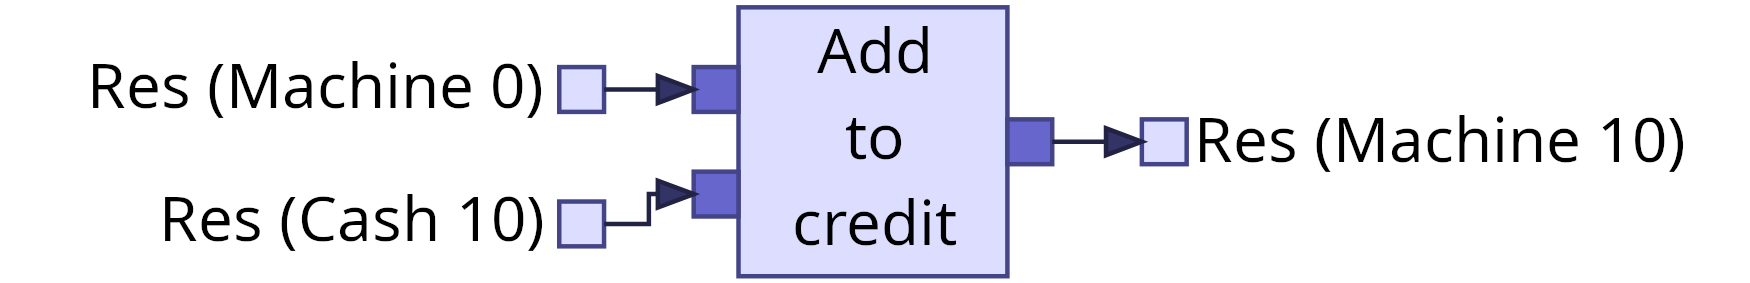
\includegraphics[scale=0.2]{img/add_to_credit_port_graph.png}
  \caption{Port graph \isa{nodePortGraph\ \isalist{}\ \isaString{Add\ to\ credit}\ \isalist{Res\ \isapars{Machine\ 0},\ Res\ \isapars{Cash\ 10}}\ \isalist{Res\ \isapars{Machine\ 10}}}, representing an instance of the \isa{add{\isacharunderscore}to{\isacharunderscore}credit} from Definition~\ref{isa:add_to_credit}.}
  \label{fig:node_port_graph}
\end{figure}

\subsection{Juxtaposition}
\label{sec:port_graphs/mech/par}

Our first complex operation on port graphs is \emph{juxtaposition}, which we will use to represent parallel composition of processes (see Section~\ref{sec:port_graphs/process/constr}).
Informally, it is very simple: take the nodes, edges and open ports of two port graphs and put them into one.
The formal definition, however, needs to be careful about potential clashes when unifying that data.

The first possible clash, and the easiest to solve, is over nodes of the two input port graphs.
We simply assume that the port graphs are disjoint, as characterised by the \isa{pg{\isacharunderscore}disjoint} relation defined in Section~\ref{sec:port_graphs/mech/data}.
To ensure the latter is satisfied before we perform this operation, we can use distinct name atoms to qualify the two port graphs apart (we do so in Section~\ref{sec:port_graphs/process/constr}).

The second possible clash involves the open ports.
Because these ports are identified by their side and the index within, we can avoid the clash by shifting the indices of open ports from one of the input port graphs.
We choose to shift those of the second input, increasing the index of every open port coming from it by the number of open ports on that side coming from the first input.
Since, in a well-formed port graph (see Section~\ref{sec:port_graphs/mech/base_locale}), the number of ports on a side is the upper bound for their index, we know shifting up by that amount will avoid any clash.
Note that this change needs to be done not just in the open ports themselves, but also in any edges that may be adjacent to them.

The last possible clash is with the edges.
However, because edges are pairs of places, which in turn are either ports of nodes or open ports, any potential clashes in them will be taken care of by the adjustments we make to nodes and open ports.

With these considerations in mind, our definition of juxtaposition of port graphs in Isabelle/HOL is as follows:
\begin{isadef}[Juxtaposing port graph]{isa:juxtapose}
  \isacomm{fun}\ juxtapose\ {\isacharcolon}{\isacharcolon}\ {\isachardoublequoteopen}{\isacharparenleft}\isatv{s}\ {\isacharcolon}{\isacharcolon}\ side{\isacharunderscore}in{\isacharunderscore}out{\isacharcomma}\ \isatv{a}{\isacharcomma}\ \isatv{p}{\isacharcomma}\ \isatv{l}{\isacharparenright}\ port{\isacharunderscore}graph\ {\isasymRightarrow}\ {\isacharparenleft}\isatv{s}{\isacharcomma}\ \isatv{a}{\isacharcomma}\ \isatv{p}{\isacharcomma}\ \isatv{l}{\isacharparenright}\ port{\isacharunderscore}graph\isanewline
\isaindent{\isacomm{fun}\ juxtapose\ }{\isasymRightarrow}\ {\isacharparenleft}\isatv{s}{\isacharcomma}\ \isatv{a}{\isacharcomma}\ \isatv{p}{\isacharcomma}\ \isatv{l}{\isacharparenright}\ port{\isacharunderscore}graph{\isachardoublequoteclose}\isanewline
\ \ \isaOcomm{where}\ {\isachardoublequoteopen}\isafv{juxtapose}\ \isabv{x\ y}\ {\isacharequal}\ PGraph\isanewline
\ \ \ \ {\isacharparenleft}\ pg{\isacharunderscore}nodes\ \isabv{x}\ {\isacharat}\ pg{\isacharunderscore}nodes\ \isabv{y}{\isacharparenright}\isanewline
\ \ \ \ {\isacharparenleft}\ pg{\isacharunderscore}edges\ \isabv{x}\ {\isacharat}\isanewline
\ \ \ \ \ \ map\ {\isacharparenleft}shiftOpenInEdge\ {\isacharparenleft}{\isasymlambda}\isabv{s}{\isachardot}\ length\ {\isacharparenleft}filter\ {\isacharparenleft}{\isasymlambda}\isabv{p}{\isachardot}\ port{\isachardot}side\ \isabv{p}\ {\isacharequal}\ \isabv{s}{\isacharparenright}\ {\isacharparenleft}pg{\isacharunderscore}ports\   \isabv{x}{\isacharparenright}{\isacharparenright}{\isacharparenright}\isanewline
\isaindent{\ \ \ \ \ \ map\ {\isacharparenleft}shiftOpenInEdge\ }{\isacharparenleft}{\isasymlambda}\isabv{s}{\isachardot}\ length\ {\isacharparenleft}filter\ {\isacharparenleft}{\isasymlambda}\isabv{p}{\isachardot}\ port{\isachardot}side\ \isabv{p}\ {\isacharequal}\ \isabv{s}{\isacharparenright}\ {\isacharparenleft}pg{\isacharunderscore}ports\   \isabv{x}{\isacharparenright}{\isacharparenright}{\isacharparenright}{\isacharparenright}\isanewline
\isaindent{\ \ \ \ \ \ map\ }{\isacharparenleft}pg{\isacharunderscore}edges\ \isabv{y}{\isacharparenright}{\isacharparenright}\isanewline
\ \ \ \ {\isacharparenleft}\ pg{\isacharunderscore}ports\ \isabv{x}\ {\isacharat}\isanewline
\ \ \ \ \ \ map\ {\isacharparenleft}shiftPort\ {\isacharparenleft}{\isasymlambda}\isabv{s}{\isachardot}\ length\ {\isacharparenleft}filter\ {\isacharparenleft}{\isasymlambda}\isabv{p}{\isachardot}\ port{\isachardot}side\ \isabv{p}\ {\isacharequal}\ \isabv{s}{\isacharparenright}\ {\isacharparenleft}pg{\isacharunderscore}ports\ \isabv{x}{\isacharparenright}{\isacharparenright}{\isacharparenright}{\isacharparenright}\isanewline
\isaindent{\ \ \ \ \ \ map\ }{\isacharparenleft}pg{\isacharunderscore}ports\ \isabv{y}{\isacharparenright}{\isacharparenright}{\isachardoublequoteclose}%

\end{isadef}
\noindent
where \isa{shiftPort} and \isa{shiftOpenInEdge} shift indices of ports, either directly or applying to any open ports contained in an edge.
The amount each port is shifted by is a function of that port's side, allowing for more concise statements.

Figure~\ref{fig:juxtapose} illustrates juxtaposition of two simple port graphs representing primitive actions (see the example introduced in Figure~\ref{fig:node_port_graph}).
The resulting port graph now has three open input ports and three open output ports.
Consider, for instance, the open output port labelled with \isa{Res\ D}.
It starts with index \isa{\isadigit{0}} in its original port graph but has index \isa{\isadigit{1}} after juxtaposition due to the open output port in the other port graph.
In Section~\ref{sec:port_graphs/process/constr}, where we use juxtaposition to represent parallel composition of processes, we also ensure the constituent port graphs are disjoint by qualifying them with distinct name atoms.

\begin{figure}[htbp]
  \centering
  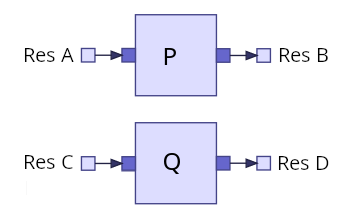
\includegraphics[scale=0.4]{img/par_port_graph_simpler.png}
  \caption{Juxtaposition of two port graphs, which we use to represent parallel composition (see Section~\ref{sec:port_graphs/process/constr}).}
  \label{fig:juxtapose}
\end{figure}

The first property we verify is that this operation preserves the port graph locales we defined.
We state this as the following two theorems, each proven by proving the relevant locale's assumptions:
\begin{isalemma}[Juxtaposition preserves well-formedness]{isa:port_graph_juxtapose}
  \begin{minipage}{0.49\textwidth}
    \isacomm{lemma}\ port{\isacharunderscore}graph{\isacharunderscore}juxtapose{\isacharcolon}\isanewline
\ \ \ \ \isaOcomm{fixes}\ \isafv{x\ y}\ {\isacharcolon}{\isacharcolon}\isanewline
\isaindent{\ \ \ \ \isaOcomm{f}}{\isachardoublequoteopen}{\isacharparenleft}\isatv{s}{\isacharcomma}\ \isatv{a}{\isacharcomma}\ \isatv{p}{\isacharcomma}\ \isatv{l}{\isacharparenright}\ port{\isacharunderscore}graph{\isachardoublequoteclose}\isanewline
\ \ \isaOcomm{assumes}\ {\isachardoublequoteopen}port{\isacharunderscore}graph\ \isafv{x}{\isachardoublequoteclose}\isanewline
\ \ \ \ \ \ \ \ \ \ \isaOcomm{and}\ {\isachardoublequoteopen}port{\isacharunderscore}graph\ \isafv{y}{\isachardoublequoteclose}\isanewline
\ \ \ \ \ \ \ \ \ \ \isaOcomm{and}\ {\isachardoublequoteopen}pg{\isacharunderscore}disjoint\ \isafv{x\ y}{\isachardoublequoteclose}\isanewline
\ \ \ \ \ \ \isaOcomm{shows}\ {\isachardoublequoteopen}port{\isacharunderscore}graph\ {\isacharparenleft}juxtapose\ \isafv{x\ y}{\isacharparenright}{\isachardoublequoteclose}

  \end{minipage}
  \vrule\kern5pt
  \begin{minipage}{0.49\textwidth}
    \isacomm{lemma}\ port{\isacharunderscore}graph{\isacharunderscore}flow{\isacharunderscore}juxtapose{\isacharcolon}\isanewline
\ \ \ \ \isaOcomm{fixes}\ \isafv{x\ y}\ {\isacharcolon}{\isacharcolon}\isanewline
\isaindent{\ \ \ \ \isaOcomm{f}}{\isachardoublequoteopen}{\isacharparenleft}\isatv{s}\ {\isacharcolon}{\isacharcolon}\ side{\isacharunderscore}in{\isacharunderscore}out{\isacharcomma}\ \isatv{a}{\isacharcomma}\ \isatv{p}{\isacharcomma}\ \isatv{l}{\isacharparenright}\ port{\isacharunderscore}graph{\isachardoublequoteclose}\isanewline
\ \ \isaOcomm{assumes}\ {\isachardoublequoteopen}port{\isacharunderscore}graph{\isacharunderscore}flow\ \isafv{x}{\isachardoublequoteclose}\isanewline
\ \ \ \ \ \ \ \ \ \ \isaOcomm{and}\ {\isachardoublequoteopen}port{\isacharunderscore}graph{\isacharunderscore}flow\ \isafv{y}{\isachardoublequoteclose}\isanewline
\ \ \ \ \ \ \ \ \ \ \isaOcomm{and}\ {\isachardoublequoteopen}pg{\isacharunderscore}disjoint\ \isafv{x\ y}{\isachardoublequoteclose}\isanewline
\ \ \ \ \ \ \isaOcomm{shows}\ {\isachardoublequoteopen}port{\isacharunderscore}graph{\isacharunderscore}flow\ {\isacharparenleft}juxtapose\ \isafv{x\ y}{\isacharparenright}{\isachardoublequoteclose}

  \end{minipage}
\end{isalemma}

Next we verify that the operation is associative up to the port graph equivalence.
We prove this according to the definition of port graph equivalence (Definition~\ref{isa:pgEquiv}): both sides are well-formed port graphs with the same set of open ports, and with nodes and edges related by renaming.
By assuming that the corresponding component port graphs are equivalent, we know that there are renaming functions between them.
We use these to form the combined renaming function and show that it relates the nodes and edges correctly.
By assuming that the component port graphs are disjoint, we can determine the source of every node in the two new port graphs and, by extension, the appropriate renaming to apply.
We state the theorem as follows:
\begin{isalemma}[Juxtaposition is associative up to equivalence]{isa:juxtapose_assoc_pgEquiv}
  \isacomm{lemma}\ juxtapose{\isacharunderscore}assoc{\isacharunderscore}pgEquiv{\isacharcolon}\isanewline
\ \ \ \ \ \ \ \ \isaOcomm{fixes}\ \isafv{x\ y\ z}\ {\isacharcolon}{\isacharcolon}\ {\isachardoublequoteopen}{\isacharparenleft}\isatv{s}{\isacharcomma}\ \isatv{a}{\isacharcomma}\ \isatv{p}{\isacharcomma}\ \isatv{l}{\isacharparenright}\ port{\isacharunderscore}graph{\isachardoublequoteclose}\isanewline
\ \ \isaOcomm{assumes}\ {\isachardoublequoteopen}port{\isacharunderscore}graph\ \isafv{x}{\isachardoublequoteclose}\ \isaOcomm{and}\ {\isachardoublequoteopen}port{\isacharunderscore}graph\ \isafv{y}{\isachardoublequoteclose} \isaOcomm{and}\ {\isachardoublequoteopen}port{\isacharunderscore}graph\ \isafv{z}{\isachardoublequoteclose}\isanewline
\ \ \ \ \ \ \ \ \ \ \isaOcomm{and}\ {\isachardoublequoteopen}pg{\isacharunderscore}disjoint\ \isafv{x\ y}{\isachardoublequoteclose}\ \isaOcomm{and}\ {\isachardoublequoteopen}pg{\isacharunderscore}disjoint\ \isafv{y\ z}{\isachardoublequoteclose} \isaOcomm{and}\ {\isachardoublequoteopen}pg{\isacharunderscore}disjoint\ \isafv{x\ z}{\isachardoublequoteclose}\isanewline
\ \ \ \ \ \ \ \ \ \ \isaOcomm{and}\ {\isachardoublequoteopen}port{\isacharunderscore}graph\ \isafv{x{\isacharprime}}{\isachardoublequoteclose}\ \isaOcomm{and}\ {\isachardoublequoteopen}port{\isacharunderscore}graph\ \isafv{y{\isacharprime}}{\isachardoublequoteclose}\ \isaOcomm{and}\ {\isachardoublequoteopen}port{\isacharunderscore}graph\ \isafv{z{\isacharprime}}{\isachardoublequoteclose}\isanewline
\ \ \ \ \ \ \ \ \ \ \isaOcomm{and}\ {\isachardoublequoteopen}pg{\isacharunderscore}disjoint\ \isafv{x{\isacharprime}\ y{\isacharprime}}{\isachardoublequoteclose}\ \isaOcomm{and}\ {\isachardoublequoteopen}pg{\isacharunderscore}disjoint\ \isafv{y{\isacharprime}\ z{\isacharprime}}{\isachardoublequoteclose}\ \isaOcomm{and}\ {\isachardoublequoteopen}pg{\isacharunderscore}disjoint\ \isafv{x{\isacharprime}\ z{\isacharprime}}{\isachardoublequoteclose}\isanewline
\ \ \ \ \ \ \ \ \ \ \isaOcomm{and}\ {\isachardoublequoteopen}\isafv{x}\ {\isasymapprox}\ \isafv{x{\isacharprime}}{\isachardoublequoteclose}\ \isaOcomm{and}\ {\isachardoublequoteopen}\isafv{y}\ {\isasymapprox}\ \isafv{y{\isacharprime}}{\isachardoublequoteclose}\ \isaOcomm{and}\ {\isachardoublequoteopen}\isafv{z}\ {\isasymapprox}\ \isafv{z{\isacharprime}}{\isachardoublequoteclose}\isanewline
\ \ \ \ \ \ \isaOcomm{shows}\ {\isachardoublequoteopen}juxtapose\ {\isacharparenleft}juxtapose\ \isafv{x\ y}{\isacharparenright}\ \isafv{z}\ {\isasymapprox}\ juxtapose\ \isafv{x{\isacharprime}}\ {\isacharparenleft}juxtapose\ \isafv{y{\isacharprime}\ z{\isacharprime}}{\isacharparenright}{\isachardoublequoteclose}

\end{isalemma}

Finally, we verify that juxtapositions of equivalent port graphs are themselves equivalent.
The proof takes the same general form as the associativity proof, being again a proof of equivalence using the same operation, but is rendered simpler by considering fewer port graphs (four instead of six).
We state the theorem as follows:
\begin{isalemma}[Juxtapositions of equivalent port graphs are equivalent]{isa:juxtapose_resp}
  \isacomm{lemma}\ juxtapose{\isacharunderscore}resp{\isacharcolon}\isanewline
\ \ \ \ \ \ \ \ \isaOcomm{fixes}\ \isafv{x\ y}\ {\isacharcolon}{\isacharcolon}\ {\isachardoublequoteopen}{\isacharparenleft}\isatv{s}{\isacharcomma}\ \isatv{a}{\isacharcomma}\ \isatv{p}{\isacharcomma}\ \isatv{l}{\isacharparenright}\ port{\isacharunderscore}graph{\isachardoublequoteclose}\isanewline
\ \ \isaOcomm{assumes}\ {\isachardoublequoteopen}port{\isacharunderscore}graph\ \isafv{x}{\isachardoublequoteclose}\ \isaOcomm{and}\ {\isachardoublequoteopen}port{\isacharunderscore}graph\ \isafv{y}{\isachardoublequoteclose}\ \isaOcomm{and}\ {\isachardoublequoteopen}pg{\isacharunderscore}disjoint\ \isafv{x\ y}{\isachardoublequoteclose}\isanewline
\ \ \ \ \ \ \ \ \ \ \isaOcomm{and}\ {\isachardoublequoteopen}port{\isacharunderscore}graph\ \isafv{x{\isacharprime}}{\isachardoublequoteclose}\ \isaOcomm{and}\ {\isachardoublequoteopen}port{\isacharunderscore}graph\ \isafv{y{\isacharprime}}{\isachardoublequoteclose}\ \isaOcomm{and}\ {\isachardoublequoteopen}pg{\isacharunderscore}disjoint\ \isafv{x{\isacharprime}\ y}{\isacharprime}{\isachardoublequoteclose}\isanewline
\ \ \ \ \ \ \ \ \ \ \isaOcomm{and}\ {\isachardoublequoteopen}\isafv{x}\ {\isasymapprox}\ \isafv{x{\isacharprime}}{\isachardoublequoteclose}\ \isaOcomm{and}\ {\isachardoublequoteopen}\isafv{y}\ {\isasymapprox}\ \isafv{y{\isacharprime}}{\isachardoublequoteclose}\isanewline
\ \ \ \ \ \ \isaOcomm{shows}\ {\isachardoublequoteopen}juxtapose\ \isafv{x\ y}\ {\isasymapprox}\ juxtapose\ \isafv{x{\isacharprime}\ y{\isacharprime}}{\isachardoublequoteclose}

\end{isalemma}

\subsection{Sequencing}
\label{sec:port_graphs/mech/seq}

As our second complex operation on port graphs we define their \emph{sequencing}, which makes use of port graph inputs, outputs and the flow between them.
We use this operation to represent sequential composition of processes (see Section~\ref{sec:port_graphs/process/constr}).
Sequencing goes further than juxtaposition, not just putting the port graphs together but also making new connections and removing other superseded elements.
Informally, on top of combining the port graphs into one, this operation: takes the open output ports of one port graph, matches them with open input ports of the other and ``stitches'' together the edges incident on them.
While doing this, it also applies the same methods for avoiding clashes as juxtaposition (i.e.\ assuming disjoint node names and open port shifting).

The core complexity of this operation is forming the new edges to represent the stitched connection in the result.
For this we define the helper function \isa{seqInterfaceEdges} on the two input port graphs \isa{\isafv{x}} and \isa{\isafv{y}} which:
\begin{enumerate}
  \item Forms a mapping from open output ports of \isa{\isafv{x}} to the edges in \isa{\isafv{x}} going into them.
  \item Forms a mapping from open input ports of \isa{\isafv{y}} to the edges in \isa{\isafv{y}} coming from them.
  \item For each open output port of \isa{\isafv{x}}, uses the mappings to retrieve the edge lists to be stitched: those of \isa{\isafv{x}} going into that port and those of \isa{\isafv{y}} coming from the matching open input port of \isa{\isafv{y}}.
  \item For each such pair of edge lists, form an edge for each combination going from the origin in \isa{\isafv{x}} to the destination in \isa{\isafv{y}}.
\end{enumerate}

The definition of \isa{seqInterfaceEdges} uses the mechanisation of mappings available in Isabelle/HOL, which represents them as functions from a key type to an optional value type.
For the purposes of code generation, this representation can be automatically mapped to a list of key-value pairs.
The full definition is given in Appendix~\ref{app:seqInterfaceEdges}.

\cbstart
In our proofs we mainly interact with this function through two rules: one introducing the fact that an edge is one of its results (Lemma~\ref{isa:seqInterfaceEdges_setI}) and the other decomposing this fact back to its necessary premises (Lemma~\ref{isa:seqInterfaceEdges_setD}).
Both of these tie an edge resulting from \isa{seqInterfaceEdges} to the existence of two edges, one in each input port graph, that ``meet'' at matching open ports and which, when combined, yield that edge.
Note that, since properties we wish to prove (such as the locales in Definition~\ref{isa:locale-port_graph} and Definition~\ref{isa:port_graph_flow}) disregard order of the edges, so do these two rules.
This significantly simplifies them in comparison to the function's implementation with mappings described above.
\cbend

\begin{isalemma}[Introduction rule for elements of \isa{seqInterfaceEdges}]{isa:seqInterfaceEdges_setI}
  \isacomm{lemma}\ seqInterfaceEdges{\isacharunderscore}setI{\isacharcolon}\isanewline
\ \ \ \ \ \ \ \ \isaOcomm{fixes}\ \isafv{x\ y}\ {\isacharcolon}{\isacharcolon}\ {\isachardoublequoteopen}{\isacharparenleft}\isatv{s}\ {\isacharcolon}{\isacharcolon}\ side{\isacharunderscore}in{\isacharunderscore}out{\isacharcomma}\ \isatv{a}{\isacharcomma}\ \isatv{p}{\isacharcomma}\ \isatv{l}{\isacharparenright}\ port{\isacharunderscore}graph{\isachardoublequoteclose}\isanewline
\ \ \isaOcomm{assumes}\ {\isachardoublequoteopen}port{\isacharunderscore}graph{\isacharunderscore}flow\ \isafv{x}{\isachardoublequoteclose}\isanewline
\ \ \ \ \ \ \ \ \ \ \isaOcomm{and}\ {\isachardoublequoteopen}port{\isacharunderscore}graph{\isacharunderscore}flow\ \isafv{y}{\isachardoublequoteclose}\isanewline
\ \ \ \ \ \ \ \ \ \ \isaOcomm{and}\ {\isachardoublequoteopen}edge{\isacharunderscore}from\ \isafv{e}\ {\isacharequal}\ edge{\isacharunderscore}from\ \isafv{a}{\isachardoublequoteclose}\isanewline
\ \ \ \ \ \ \ \ \ \ \isaOcomm{and}\ {\isachardoublequoteopen}\isafv{a}\ {\isasymin}\ set\ {\isacharparenleft}pg{\isacharunderscore}edges\ \isafv{x}{\isacharparenright}{\isachardoublequoteclose}\isanewline
\ \ \ \ \ \ \ \ \ \ \isaOcomm{and}\ {\isachardoublequoteopen}edge{\isacharunderscore}to\ \isafv{e}\ {\isacharequal}\ edge{\isacharunderscore}to\ \isafv{b}{\isachardoublequoteclose}\isanewline
\ \ \ \ \ \ \ \ \ \ \isaOcomm{and}\ {\isachardoublequoteopen}\isafv{b}\ {\isasymin}\ set\ {\isacharparenleft}pg{\isacharunderscore}edges\ \isafv{y}{\isacharparenright}{\isachardoublequoteclose}\isanewline
\ \ \ \ \ \ \ \ \ \ \isaOcomm{and}\ {\isachardoublequoteopen}edge{\isacharunderscore}to\ \isafv{a}\ {\isacharequal}\ OpenPort\ {\isacharparenleft}portSetSide\ Out\ \isafv{p}{\isacharparenright}{\isachardoublequoteclose}\isanewline
\ \ \ \ \ \ \ \ \ \ \isaOcomm{and}\ {\isachardoublequoteopen}edge{\isacharunderscore}from\ \isafv{b}\ {\isacharequal}\ OpenPort\ {\isacharparenleft}portSetSide\ In\ \isafv{p}{\isacharparenright}{\isachardoublequoteclose}\isanewline
\ \ \ \ \ \ \ \ \ \ \isaOcomm{and}\ {\isachardoublequoteopen}port{\isachardot}side\ \isafv{p}\ \isacharequal\ Out{\isachardoublequoteclose}\isanewline
\ \ \ \ \ \ \isaOcomm{shows}\ {\isachardoublequoteopen}\isafv{e}\ {\isasymin}\ set\ {\isacharparenleft}seqInterfaceEdges\ \isafv{x\ y}{\isacharparenright}{\isachardoublequoteclose}

\end{isalemma}
\pagebreak
\begin{isalemma}[Destruction rule for elements of \isa{seqInterfaceEdges}]{isa:seqInterfaceEdges_setD}
  \isacomm{lemma}\ seqInterfaceEdges{\isacharunderscore}setD{\isacharcolon}\isanewline
\ \ \ \ \ \ \ \ \isaOcomm{fixes}\ \isafv{x\ y}\ {\isacharcolon}{\isacharcolon}\ {\isachardoublequoteopen}{\isacharparenleft}\isatv{s}\ {\isacharcolon}{\isacharcolon}\ side{\isacharunderscore}in{\isacharunderscore}out{\isacharcomma}\ \isatv{a}{\isacharcomma}\ \isatv{p}{\isacharcomma}\ \isatv{l}{\isacharparenright}\ port{\isacharunderscore}graph{\isachardoublequoteclose}\isanewline
\ \ \isaOcomm{assumes}\ {\isachardoublequoteopen}\isafv{e}\ {\isasymin}\ set\ {\isacharparenleft}seqInterfaceEdges\ \isafv{x\ y}{\isacharparenright}{\isachardoublequoteclose}\isanewline
\ \ \ \ \isaOcomm{obtains}\ \isafv{a\ b}\ \isaOcomm{and}\ \isafv{p}\ {\isacharcolon}{\isacharcolon}\ {\isachardoublequoteopen}{\isacharparenleft}\isatv{s}{\isacharcomma}\ \isatv{a}{\isacharparenright}\ port{\isachardoublequoteclose}\isanewline
\ \ \ \ \ \ \isaOcomm{where}\ {\isachardoublequoteopen}edge{\isacharunderscore}from\ \isafv{e}\ {\isacharequal}\ edge{\isacharunderscore}from\ \isafv{a}{\isachardoublequoteclose}\isanewline
\ \ \ \ \ \ \ \ \ \ \isaOcomm{and}\ {\isachardoublequoteopen}\isafv{a}\ {\isasymin}\ set\ {\isacharparenleft}pg{\isacharunderscore}edges\ \isafv{x}{\isacharparenright}{\isachardoublequoteclose}\isanewline
\ \ \ \ \ \ \ \ \ \ \isaOcomm{and}\ {\isachardoublequoteopen}edge{\isacharunderscore}to\ \isafv{e}\ {\isacharequal}\ edge{\isacharunderscore}to\ \isafv{b}{\isachardoublequoteclose}\isanewline
\ \ \ \ \ \ \ \ \ \ \isaOcomm{and}\ {\isachardoublequoteopen}\isafv{b}\ {\isasymin}\ set\ {\isacharparenleft}pg{\isacharunderscore}edges\ \isafv{y}{\isacharparenright}{\isachardoublequoteclose}\isanewline
\ \ \ \ \ \ \ \ \ \ \isaOcomm{and}\ {\isachardoublequoteopen}edge{\isacharunderscore}to\ \isafv{a}\ {\isacharequal}\ OpenPort\ {\isacharparenleft}portSetSide\ Out\ \isafv{p}{\isacharparenright}{\isachardoublequoteclose}\isanewline
\ \ \ \ \ \ \ \ \ \ \isaOcomm{and}\ {\isachardoublequoteopen}edge{\isacharunderscore}from\ \isafv{b}\ {\isacharequal}\ OpenPort\ {\isacharparenleft}portSetSide\ In\ \isafv{p}{\isacharparenright}{\isachardoublequoteclose}\isanewline
\ \ \ \ \ \ \ \ \ \ \isaOcomm{and}\ {\isachardoublequoteopen}port{\isachardot}side\ \isafv{p}\ {\isacharequal}\ Out{\isachardoublequoteclose}

\end{isalemma}

With the edges that stitch together the output-input connection, we no longer need the original edges or the open ports used.
To remove the open ports we simply filter them out.
To remove the edges we use the helper function \isa{disconnectFromPlaces~\isafv{ps}~\isafv{es}} which filters the edges \isa{\isafv{es}} to remove any that are incident on a place in \isa{\isafv{ps}}.

\begin{isadef}[Removing edges adjacent on given places]{isa:disconnectFromPlaces}
  \isacomm{definition}\ disconnectFromPlaces\ {\isacharcolon}{\isacharcolon}\ {\isachardoublequoteopen}{\isacharparenleft}\isatv{s}{\isacharcomma}\ \isatv{a}{\isacharcomma}\ \isatv{p}{\isacharparenright}\ place\ list\ {\isasymRightarrow}\ {\isacharparenleft}\isatv{s}{\isacharcomma}\ \isatv{a}{\isacharcomma}\ \isatv{p}{\isacharparenright}\ edge\ list\isanewline
\isaindent{\isacomm{definition}\ disconnectFromPlaces\ }{\isasymRightarrow}\ {\isacharparenleft}\isatv{s}{\isacharcomma}\ \isatv{a}{\isacharcomma}\ \isatv{p}{\isacharparenright}\ edge\ list{\isachardoublequoteclose}\isanewline
\ \ \isaOcomm{where}\ {\isachardoublequoteopen}\isafv{disconnectFromPlaces}\ \isabv{ps\ es}\ {\isacharequal}\isanewline
\ \ \ \ filter\ {\isacharparenleft}{\isasymlambda}\isabv{e}{\isachardot}\ edge{\isacharunderscore}from\ \isabv{e}\ {\isasymnotin}\ set\ \isabv{ps}\ {\isasymand}\ edge{\isacharunderscore}to\ \isabv{e}\ {\isasymnotin}\ set\ \isabv{ps}{\isacharparenright}\ \isabv{es}{\isachardoublequoteclose}

\end{isadef}

Note that these removals need to be taken into account when shifting open ports (and their occurrences in edges) to avoid clashes: one port graph contributes no output and the other contributes no inputs, so only ports on other sides need to be shifted up.

Our definition of port graph sequencing in Isabelle/HOL is shown in Definition~\ref{isa:seqPortGraphs}.
\cbstart
To form the nodes of the result, it simply appends the two lists (line 4).
The edges of the result are split into three groups: first are the new edges forming the connection between the two port graphs (line 5), then the edges of the first port graph except for those that were going to its open outputs (lines 6--8), and finally the edges of the second port graph except for those coming from its open inputs and with the appropriate shifting of indices applied (lines 9--16).
This shifting of indices applies to open ports that are neither inputs nor outputs, and ensures that there can be no clash in open ports coming from the two input port graphs.
Finally, the ports of the result are also split into three groups: all non-output ports of the first port graph (line 17), all output ports of the second port graph (line 18), and all other ports of the second port graph with their indices shifted in the same way (lines 19--20).
\cbend

\begin{isadef}[Sequencing of port graphs]{isa:seqPortGraphs}
  \begin{linenumbers*}
    \isacomm{fun}\ seqPortGraphs\ {\isacharcolon}{\isacharcolon}\ {\isachardoublequoteopen}{\isacharparenleft}\isatv{s}\ {\isacharcolon}{\isacharcolon}\ side{\isacharunderscore}in{\isacharunderscore}out{\isacharcomma}\ \isatv{a}{\isacharcomma}\ \isatv{p}{\isacharcomma}\ \isatv{l}{\isacharparenright}\ port{\isacharunderscore}graph\ {\isasymRightarrow}\ {\isacharparenleft}\isatv{s}{\isacharcomma}\ \isatv{a}{\isacharcomma}\ \isatv{p}{\isacharcomma}\ \isatv{l}{\isacharparenright}\ port{\isacharunderscore}graph\isanewline
\isaindent{\isacomm{fun}\ seqPortGraphs\ }{\isasymRightarrow}\ {\isacharparenleft}\isatv{s}{\isacharcomma}\ \isatv{a}{\isacharcomma}\ \isatv{p}{\isacharcomma}\ \isatv{l}{\isacharparenright}\ port{\isacharunderscore}graph{\isachardoublequoteclose}\isanewline
\ \ \isaOcomm{where}\ {\isachardoublequoteopen}\isafv{seqPortGraphs}\ \isabv{x\ y}\ {\isacharequal}\ PGraph\isanewline
\ \ \ \ {\isacharparenleft}\ pg{\isacharunderscore}nodes\ \isabv{x}\ {\isacharat}\ pg{\isacharunderscore}nodes\ \isabv{y}{\isacharparenright}\isanewline
\ \ \ \ {\isacharparenleft}\ seqInterfaceEdges\ \isabv{x\ y}\ {\isacharat}\isanewline
\ \ \ \ \ \ disconnectFromPlaces\isanewline
\isaindent{\ \ \ \ \ \ di}{\isacharparenleft}map\ OpenPort\ {\isacharparenleft}filter\ {\isacharparenleft}{\isasymlambda}\isabv{x}{\isachardot}\ port{\isachardot}side\ \isabv{x}\ {\isacharequal}\ Out{\isacharparenright}\ {\isacharparenleft}pg{\isacharunderscore}ports\ \isabv{x}{\isacharparenright}{\isacharparenright}{\isacharparenright}\isanewline
\isaindent{\ \ \ \ \ \ di}{\isacharparenleft}pg{\isacharunderscore}edges\ \isabv{x}{\isacharparenright}\ {\isacharat}\isanewline
\ \ \ \ \ \ map\ {\isacharparenleft}shiftOpenInEdge\isanewline
\isaindent{\ \ \ \ \ \ map\ {\isacharparenleft}sh}{\isacharparenleft}{\isasymlambda}\isabv{s}{\isachardot}\ \isanotation{if}\ \isabv{s}\ {\isacharequal}\ In\ {\isasymor}\ \isabv{s}\ {\isacharequal}\ Out\ \isanotation{then}\ {\isadigit{0}}\isanewline
\isaindent{\ \ \ \ \ \ map\ {\isacharparenleft}sh{\isacharparenleft}{\isasymlambda}\isabv{s}{\isachardot}\ }\isanotation{else}\ length\ {\isacharparenleft}filter\ {\isacharparenleft}{\isasymlambda}\isabv{x}{\isachardot}\ port{\isachardot}side\ \isabv{x}\ {\isacharequal}\ \isabv{s}{\isacharparenright}\ {\isacharparenleft}pg{\isacharunderscore}ports\ \isabv{x}{\isacharparenright}{\isacharparenright}{\isacharparenright}\isanewline
\isaindent{\ \ \ \ \ \ map\ {\isacharparenleft}sh}{\isacharparenleft}{\isasymlambda}\isabv{s}{\isachardot}\ \isanotation{if}\ \isabv{s}\ {\isacharequal}\ In\ {\isasymor}\ \isabv{s}\ {\isacharequal}\ Out\ \isanotation{then}\ {\isadigit{0}}\isanewline
\isaindent{\ \ \ \ \ \ map\ {\isacharparenleft}sh{\isacharparenleft}{\isasymlambda}\isabv{s}{\isachardot}\ }\isanotation{else}\ length\ {\isacharparenleft}filter\ {\isacharparenleft}{\isasymlambda}\isabv{x}{\isachardot}\ port{\isachardot}side\ \isabv{x}\ {\isacharequal}\ \isabv{s}{\isacharparenright}\ {\isacharparenleft}pg{\isacharunderscore}ports\ \isabv{x}{\isacharparenright}{\isacharparenright}{\isacharparenright}{\isacharparenright}\isanewline
\isaindent{\ \ \ \ \ \ map\ }{\isacharparenleft}disconnectFromPlaces\isanewline
\isaindent{\ \ \ \ \ \ map\ {\isacharparenleft}di}{\isacharparenleft}map\ OpenPort\ {\isacharparenleft}filter\ {\isacharparenleft}{\isasymlambda}\isabv{x}{\isachardot}\ port{\isachardot}side\ \isabv{x}\ {\isacharequal}\ In{\isacharparenright}\ {\isacharparenleft}pg{\isacharunderscore}ports\ \isabv{y}{\isacharparenright}{\isacharparenright}{\isacharparenright}\isanewline
\isaindent{\ \ \ \ \ \ map\ {\isacharparenleft}di}{\isacharparenleft}pg{\isacharunderscore}edges\ \isabv{y}{\isacharparenright}{\isacharparenright}{\isacharparenright}\isanewline
\ \ \ \ {\isacharparenleft}\ filter\ {\isacharparenleft}{\isasymlambda}\isabv{x}{\isachardot}\ port{\isachardot}side\ \isabv{x}\ {\isasymnoteq}\ Out{\isacharparenright}\ {\isacharparenleft}pg{\isacharunderscore}ports\ \isabv{x}{\isacharparenright}\ {\isacharat}\isanewline
\ \ \ \ \ \ filter\ {\isacharparenleft}{\isasymlambda}\isabv{x}{\isachardot}\ port{\isachardot}side\ \isabv{x}\ {\isacharequal}\ Out{\isacharparenright}\ {\isacharparenleft}pg{\isacharunderscore}ports\ \isabv{y}{\isacharparenright}\ {\isacharat}\isanewline
\ \ \ \ \ \ map\ {\isacharparenleft}shiftPort\ {\isacharparenleft}{\isasymlambda}\isabv{s}{\isachardot}\ length\ {\isacharparenleft}filter\ {\isacharparenleft}{\isasymlambda}\isabv{p}{\isachardot}\ port{\isachardot}side\ \isabv{p}\ {\isacharequal}\ \isabv{s}{\isacharparenright}\ {\isacharparenleft}pg{\isacharunderscore}ports\ \isabv{x}{\isacharparenright}{\isacharparenright}{\isacharparenright}{\isacharparenright}\isanewline
\ \ \ \ \ \ \isaindent{map}\ {\isacharparenleft}filter\ {\isacharparenleft}{\isasymlambda}\isabv{x}{\isachardot}\ port{\isachardot}side\ \isabv{x}\ {\isasymnoteq}\ In\ {\isasymand}\ port{\isachardot}side\ \isabv{x}\ {\isasymnoteq}\ Out{\isacharparenright}\ {\isacharparenleft}pg{\isacharunderscore}ports\ \isabv{y}{\isacharparenright}{\isacharparenright}{\isacharparenright}{\isachardoublequoteclose}%

  \end{linenumbers*}
\end{isadef}

Figure~\ref{fig:seqPortGraphs} illustrates sequencing of the same simple port graphs as our example of juxtaposition in Figure~\ref{fig:juxtapose}.
The resulting port graph now only has one open input port and one open output port.
The open ports labelled \isa{Res\ B} and \isa{Res\ C} in the original port graphs are stitched together by \isa{seqInterfaceEdges} to form two edges between ground ports instead.
As with juxtaposition, in Section~\ref{sec:port_graphs/process/constr} we qualify the constituent port graphs to ensure they are disjoint.

\begin{figure}[htb]
  \centering
  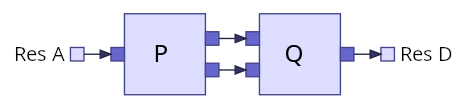
\includegraphics[scale=0.4]{img/seq_port_graph.png}
  \caption{Sequencing of two port graphs, which we use to represent sequential composition (see Section~\ref{sec:port_graphs/process/constr}).}
  \label{fig:seqPortGraphs}
\end{figure}

Once again, the first property we verify is that this operation preserves the port graph locales.
In this case, however, even proving that the base locale remain satisfied requires facts from the flow locale.
For instance, if an edge is part of the stitched connection, then its origin is only guaranteed to be in the port graph because we know it could not have been one of the open output ports that were removed.
More complex situations requiring facts about the flow arise as part of proving that this process does not introduce any duplicate edges.
As such, we state this as a single theorem, albeit in almost the same form as the one for juxtaposition:
\begin{isalemma}[Sequencing port graphs preserves well-formedness]{isa:port_graph_flow_seqPortGraphs}
  \isacomm{lemma}\ port{\isacharunderscore}graph{\isacharunderscore}flow{\isacharunderscore}seqPortGraphs{\isacharcolon}\isanewline
\ \ \ \ \ \ \ \ \isaOcomm{fixes}\ \isafv{x\ y}\ {\isacharcolon}{\isacharcolon}\ {\isachardoublequoteopen}{\isacharparenleft}\isatv{s}\ {\isacharcolon}{\isacharcolon}\ side{\isacharunderscore}in{\isacharunderscore}out{\isacharcomma}\ \isatv{a}{\isacharcomma}\ \isatv{p}{\isacharcomma}\ \isatv{l}{\isacharparenright}\ port{\isacharunderscore}graph{\isachardoublequoteclose}\isanewline
\ \ \isaOcomm{assumes}\ {\isachardoublequoteopen}port{\isacharunderscore}graph{\isacharunderscore}flow\ \isafv{x}{\isachardoublequoteclose}\isanewline
\ \ \ \ \ \ \ \ \ \ \isaOcomm{and}\ {\isachardoublequoteopen}port{\isacharunderscore}graph{\isacharunderscore}flow\ \isafv{y}{\isachardoublequoteclose}\isanewline
\ \ \ \ \ \ \ \ \ \ \isaOcomm{and}\ {\isachardoublequoteopen}pg{\isacharunderscore}disjoint\ \isafv{x\ y}{\isachardoublequoteclose}\isanewline
\ \ \ \ \ \ \isaOcomm{shows}\ {\isachardoublequoteopen}port{\isacharunderscore}graph{\isacharunderscore}flow\ {\isacharparenleft}seqPortGraphs\ \isafv{x\ y}{\isacharparenright}{\isachardoublequoteclose}

\end{isalemma}

The other two properties, namely that the operation is associative and respects port graph equivalence, are stated in the same form as those for juxtaposition except for the port graphs needing to satisfy the stronger \isa{port{\isacharunderscore}graph{\isacharunderscore}flow} locale.
It is the proofs of these properties that are made more complex due to the operation being more complex.
For instance, when proving that edges of the two resulting port graphs are related by renaming, we need to consider more cases: an edge could come from any of the constituent port graphs or be the result of one of the stitched interfaces.
In each case we need to find the corresponding edge in the other resulting port graph and show that the combined renaming function indeed relates them.
\begin{isalemma}[Sequencing is associative up to equivalence]{isa:seqPortGraphs_assoc_pgEquiv}
  \isacomm{lemma}\ seqPortGraphs{\isacharunderscore}assoc{\isacharunderscore}pgEquiv{\isacharcolon}\isanewline
\ \ \ \ \ \ \ \ \isaOcomm{fixes}\ \isafv{x\ y\ z}\ {\isacharcolon}{\isacharcolon}\ {\isachardoublequoteopen}{\isacharparenleft}\isatv{s}\ {\isacharcolon}{\isacharcolon}\ side{\isacharunderscore}in{\isacharunderscore}out{\isacharcomma}\ \isatv{a}{\isacharcomma}\ \isatv{p}{\isacharcomma}\ \isatv{l}{\isacharparenright}\ port{\isacharunderscore}graph{\isachardoublequoteclose}\isanewline
\ \ \isaOcomm{assumes}\ {\isachardoublequoteopen}port{\isacharunderscore}graph{\isacharunderscore}flow\ \isafv{x}{\isachardoublequoteclose}\ \isaOcomm{and}\ {\isachardoublequoteopen}port{\isacharunderscore}graph{\isacharunderscore}flow\ \isafv{y}{\isachardoublequoteclose} \isaOcomm{and}\ {\isachardoublequoteopen}port{\isacharunderscore}graph{\isacharunderscore}flow\ \isafv{z}{\isachardoublequoteclose}\isanewline
\ \ \ \ \ \ \ \ \ \ \isaOcomm{and}\ {\isachardoublequoteopen}pg{\isacharunderscore}disjoint\ \isafv{x\ y}{\isachardoublequoteclose}\ \isaOcomm{and}\ {\isachardoublequoteopen}pg{\isacharunderscore}disjoint\ \isafv{y\ z}{\isachardoublequoteclose} \isaOcomm{and}\ {\isachardoublequoteopen}pg{\isacharunderscore}disjoint\ \isafv{x\ z}{\isachardoublequoteclose}\isanewline
\ \ \ \ \ \ \ \ \ \ \isaOcomm{and}\ {\isachardoublequoteopen}port{\isacharunderscore}graph{\isacharunderscore}flow\ \isafv{x{\isacharprime}}{\isachardoublequoteclose}\ \isaOcomm{and}\ {\isachardoublequoteopen}port{\isacharunderscore}graph{\isacharunderscore}flow\ \isafv{y{\isacharprime}}{\isachardoublequoteclose}\ \isaOcomm{and}\ {\isachardoublequoteopen}port{\isacharunderscore}graph{\isacharunderscore}flow\ \isafv{z{\isacharprime}}{\isachardoublequoteclose}\isanewline
\ \ \ \ \ \ \ \ \ \ \isaOcomm{and}\ {\isachardoublequoteopen}pg{\isacharunderscore}disjoint\ \isafv{x{\isacharprime}\ y{\isacharprime}}{\isachardoublequoteclose}\ \isaOcomm{and}\ {\isachardoublequoteopen}pg{\isacharunderscore}disjoint\ \isafv{y{\isacharprime}\ z{\isacharprime}}{\isachardoublequoteclose}\ \isaOcomm{and}\ {\isachardoublequoteopen}pg{\isacharunderscore}disjoint\ \isafv{x{\isacharprime}\ z{\isacharprime}}{\isachardoublequoteclose}\isanewline
\ \ \ \ \ \ \ \ \ \ \isaOcomm{and}\ {\isachardoublequoteopen}\isafv{x}\ {\isasymapprox}\ \isafv{x{\isacharprime}}{\isachardoublequoteclose}\ \isaOcomm{and}\ {\isachardoublequoteopen}\isafv{y}\ {\isasymapprox}\ \isafv{y{\isacharprime}}{\isachardoublequoteclose}\ \isaOcomm{and}\ {\isachardoublequoteopen}\isafv{z}\ {\isasymapprox}\ \isafv{z{\isacharprime}}{\isachardoublequoteclose}\isanewline
\ \ \ \ \ \ \isaOcomm{shows}\ {\isachardoublequoteopen}seqPortGraphs\ {\isacharparenleft}seqPortGraphs\ \isafv{x\ y}{\isacharparenright}\ \isafv{z}\ {\isasymapprox}\isanewline
\isaindent{\ \ \ \ \ \ \isaOcomm{shows}\ {\isachardoublequoteopen}}seqPortGraphs\ \isafv{x{\isacharprime}}\ {\isacharparenleft}seqPortGraphs\ \isafv{y{\isacharprime}\ z{\isacharprime}}{\isacharparenright}{\isachardoublequoteclose}

\end{isalemma}
\begin{isalemma}[Sequencings of equivalent port graphs are equivalent]{isa:seqPortGraphs_resp}
  \isacomm{lemma}\ seqPortGraphs{\isacharunderscore}resp{\isacharcolon}\isanewline
\ \ \ \ \ \ \ \ \isaOcomm{fixes}\ \isafv{x\ y}\ {\isacharcolon}{\isacharcolon}\ {\isachardoublequoteopen}{\isacharparenleft}\isatv{s}\ {\isacharcolon}{\isacharcolon}\ side{\isacharunderscore}in{\isacharunderscore}out{\isacharcomma}\ \isatv{a}{\isacharcomma}\ \isatv{p}{\isacharcomma}\ \isatv{l}{\isacharparenright}\ port{\isacharunderscore}graph{\isachardoublequoteclose}\isanewline
\ \ \isaOcomm{assumes}\ {\isachardoublequoteopen}port{\isacharunderscore}graph{\isacharunderscore}flow\ \isafv{x}{\isachardoublequoteclose}\ \isaOcomm{and}\ {\isachardoublequoteopen}port{\isacharunderscore}graph{\isacharunderscore}flow\ \isafv{y}{\isachardoublequoteclose}\ \isaOcomm{and}\ {\isachardoublequoteopen}pg{\isacharunderscore}disjoint\ \isafv{x\ y}{\isachardoublequoteclose}\isanewline
\ \ \ \ \ \ \ \ \ \ \isaOcomm{and}\ {\isachardoublequoteopen}port{\isacharunderscore}graph{\isacharunderscore}flow\ \isafv{x{\isacharprime}}{\isachardoublequoteclose}\ \isaOcomm{and}\ {\isachardoublequoteopen}port{\isacharunderscore}graph{\isacharunderscore}flow\ \isafv{y{\isacharprime}}{\isachardoublequoteclose}\ \isaOcomm{and}\ {\isachardoublequoteopen}pg{\isacharunderscore}disjoint\ \isafv{x{\isacharprime}\ y}{\isacharprime}{\isachardoublequoteclose}\isanewline
\ \ \ \ \ \ \ \ \ \ \isaOcomm{and}\ {\isachardoublequoteopen}\isafv{x}\ {\isasymapprox}\ \isafv{x{\isacharprime}}{\isachardoublequoteclose}\ \isaOcomm{and}\ {\isachardoublequoteopen}\isafv{y}\ {\isasymapprox}\ \isafv{y{\isacharprime}}{\isachardoublequoteclose}\isanewline
\ \ \ \ \ \ \isaOcomm{shows}\ {\isachardoublequoteopen}seqPortGraphs\ \isafv{x\ y}\ {\isasymapprox}\ seqPortGraphs\ \isafv{x{\isacharprime}\ y{\isacharprime}}{\isachardoublequoteclose}

\end{isalemma}

\subsection{Port Graph Export}
\label{sec:port_graphs/mech/export}

Our mechanisation allows us to specify concrete port graphs, manipulate them and prove their properties.
However, being firmly in the algebraic environment of Isabelle, we cannot directly visualise them.
That means we miss out on a significant advantage offered by their graphical nature to human comprehension.

Outside the proof assistant there exist tools which, given the data describing a port graph, lay the individual elements out on a plane and turn it into an image.
We take advantage of this by mechanising a function from port graphs to the data such a tool needs.

We target the Eclipse Layout Kernel (ELK)~\cite{domros_et_al-2023}, which can represent (hierarchical) port graphs and implements a range of graph layout algorithms, and Eclipse Sprotty~\footnote{\url{https://projects.eclipse.org/projects/ecd.sprotty}}, which is a web-based diagramming framework compatible with ELK.
Their integration is shown by the online ELK Demonstrators~\footnote{\url{https://rtsys.informatik.uni-kiel.de/elklive/}}.

Within Isabelle/HOL, we use the existing mechanisation of JSON due to Brucker~\cite{Nano_JSON-AFP} to define a function from port graphs into an ELK-compatible JSON object.
While most of the implementation (given in full in Appendix~\ref{app:elk_export}) consists of directly turning each aspect of our port graphs into the ELK JSON counterpart, we also need to convert the type variables port graphs use into a form comprehensible to ELK.
As such, we parameterise the conversion function with the following domain-dependent functions:
\begin{itemize}
  \item Mapping of port graph sides to the five port sides that ELK supports: \texttt{UNDEFINED}, \texttt{NORTH}, \texttt{EAST}, \texttt{SOUTH}, \texttt{WEST}.
    For instance, with process port graphs we map \isa{In} to \texttt{WEST} and \isa{Out} to \texttt{EAST}.
  \item Mapping of node names to string literals, so they can be used as components in unique identifiers.
    For instance, with process port graphs we simply print the path to the relevant action in the composition tree to uniquely identify it.
  \item Mapping of node labels to string literals, so they can be used as node labels in the visualisation.
    For instance, with process port graphs we use the action's label.
\end{itemize}

Once instantiated for a specific type of port graphs, such as process port graphs, the conversion function produces formal JSON objects.
These we then turn into text and visualise using the online ELK JSON Demonstrator~\footnote{\url{https://rtsys.informatik.uni-kiel.de/elklive/json.html}}.
We use this method to visualise the port graphs in the present chapter, but in Section~\ref{sec:port_graphs/conc} we note the potential for a more closely tailored tool.

\subsection{Summary}

We have mechanised a self-contained theory of port graphs, which we will use in the following sections to graphically reason about process compositions.
It includes the data representing port graphs, constraints on that data and two significant port graph compositions.

While certainly influenced by our intention, we believe this theory is sufficiently general to be of use for formal verification in other contexts.
As noted in Section~\ref{sec:port_graphs/rel}, port graphs have been used to model biochemical processes and social networks, and are connected to graphical languages used, for instance, to reason about quantum circuits.

In the next section we specialise this general theory to our case of graphical representation of process compositions and use the language of port graphs to prove their various properties.
This perspective is particularly useful when talking about resource connections between actions.

\section{Process Port Graphs}
\label{sec:port_graphs/process}

Turning process compositions into port graphs, we use nodes to represent primitive actions and edges to represent the resource connections between those actions.
These resource connections are the result of composition operations and resource actions, which we represent with port graph operations and node-less port graphs respectively.

\cbstart
Note that with process port graphs we can use the tools described in Section~\ref{sec:port_graphs/mech/export} to visualise process compositions.
This differs in several ways from the process diagrams of Section~\ref{sec:proc/diag}.
First, as discussed in more detail in Section~\ref{sec:port_graphs/process/constr}, our construction only applies to a subset of process compositions while the process diagrams apply to all valid compositions.
However, second, the process port graphs tie compositions \emph{formally} to the graphical representation, allowing us to prove their properties, while process diagrams are informal.
Third, where both visualisations exist they will often differ in their layout, since the layout of port graphs is determined by an algorithm based on the present connections while the layout of process diagrams is determined na\"{i}vely from the composition structure.
But the connections between actions that both visualisations represent will be the same.
\cbend

We start this section by discussion of how we specialise the general type of port graphs to suit our purposes.
Then we describe the translation itself and continue on to its verified properties.
In the following section we will discuss our main theorem stemming from this translation, a graphical proof of process linearity.

\subsection{Preliminaries}
\label{sec:port_graphs/process/prelim}

Before we can even state how process compositions relate to port graphs, we need to instantiate the type variables of port graphs to specify the sides, name atoms, node labels and port labels.
We give these instantiations relative to the process composition type variables: \isa{\isatv{a}} and \isa{\isatv{b}} for linear and copyable resource atoms respectively, and \isa{\isatv{l}} and \isa{\isatv{m}} for primitive process label and metadata respectively.
\cbar{Note that, with regards to ports, the instantiation matches that of Section~\ref{sec:proc/diag/paths} for process diagrams.}

To represent process compositions we only need two sides: input and output.
\cbar{We reuse our formalisation of these sides from Section~\ref{sec:proc/diag/paths} and prove it} to be an instance of the \isa{side{\isacharunderscore}in{\isacharunderscore}out} type class from Section~\ref{sec:port_graphs/mech/flow_locale}.
\begin{isadef}[Datatype of process sides, an instance of \isa{side{\isacharunderscore}in{\isacharunderscore}out}]{isa:process_side}
  \isacomm{datatype}\ process{\isacharunderscore}side\ \isacharequal\ In\ \isacharbar\ Out

\item
  \isacomm{instantiation}\ process{\isacharunderscore}side\ \ty\ side{\isacharunderscore}in{\isacharunderscore}out\isanewline
\isaOcomm{begin}\isanewline
\ \ \isacomm{definition}\ In\ \isacharequal\ process{\isacharunderscore}side{\isachardot}In\isanewline
\ \ \isacomm{definition}\ Out\ \isacharequal\ process{\isacharunderscore}side{\isachardot}Out\isanewline
\ \ \isacomm{instance\ by}\ standard\ \isapars{simp\ \quasi{add:}\ In{\isacharunderscore}process{\isacharunderscore}side{\isacharunderscore}def\ Out{\isacharunderscore}process{\isacharunderscore}side{\isacharunderscore}def}\isanewline
\isaOcomm{end}

\end{isadef}

Nodes in this case represent primitive actions, which can be uniquely identified in a process composition by the path to that leaf.
See Section~\ref{sec:proc/diag/paths} for our earlier discussion of these paths and their formalisation, which we reuse here (reproduced in Definition~\ref{isa:process_inner-again}.
As such, the name atoms we use are the type \isa{process{\isacharunderscore}inner}.
\begin{isadef}[Components for composition tree paths]{isa:process_inner-again}
  \isacomm{datatype}\ process{\isacharunderscore}inner\ {\isacharequal}\ SeqL\ {\isacharbar}\ SeqR\ {\isacharbar}\ ParL\ {\isacharbar}\ ParR\ {\isacharbar}\ OptL\ {\isacharbar}\ OptR\ {\isacharbar}\ Rep

\end{isadef}

Furthermore, because the only nodes are primitive actions, we annotate them with the extra data of those actions.
For this we define a new datatype, \isa{\isapars{\isatv{l}{\isacharcomma}\ \isatv{m}}\ node{\isacharunderscore}content}, to collect together an action's label and metadata:
\begin{isadef}[Datatype holding node content]{isa:node_content}
  \isacomm{datatype}\ \isapars{\isatv{l}{\isacharcomma}\ \isatv{m}}\ node{\isacharunderscore}content\ \isacharequal\ NodePrimitive\ \isapars{\isatv{l}}\ \isapars{\isatv{m}}

\end{isadef}

Ports represent parallel parts of the input and output resources of an action, so we annotate them with the relevant resources.
\cbar{See our discussion of ports in the context of} process diagrams in Section~\ref{sec:proc/diag/paths}.
As such, the port labels we use are the type \isa{\isapars{\isatv{a}{\isacharcomma}\ \isatv{b}}\ resource}.

All together, the specific type of port graphs we use is the following:
\begin{isabelle}
\centering
  {\isacharparenleft}process{\isacharunderscore}side{\isacharcomma}\ {\isacharparenleft}\isatv{a}{\isacharcomma}\ \isatv{b}{\isacharparenright}\ resource{\isacharcomma}\ process{\isacharunderscore}inner{\isacharcomma}\ {\isacharparenleft}\isatv{l}{\isacharcomma}\ \isatv{m}{\isacharparenright}\ node{\isacharunderscore}content{\isacharparenright}\ port{\isacharunderscore}graph
\end{isabelle}
which we abbreviate as:
\begin{isabelle}
\centering
  {\isacharparenleft}\isatv{a}{\isacharcomma}\ \isatv{b}{\isacharcomma}\ \isatv{l}{\isacharcomma}\ \isatv{m}{\isacharparenright}\ process{\isacharunderscore}port{\isacharunderscore}graph
\end{isabelle}

\subsection{Process Port Graph Construction}
\label{sec:port_graphs/process/constr}

We construct port graphs from processes by associating each action with a port graph template and each composition operation with an operation on port graphs, as shown in Definition~\ref{isa:pgConstruct}.
\cbar{We follow it with more detailed discussion of its cases.}

\begin{isadef}[Constructing a port graph from a process composition]{isa:pgConstruct}
  \isacomm{primrec}\ pgConstruct\ {\isacharcolon}{\isacharcolon}\ {\isachardoublequoteopen}{\isacharparenleft}\isatv{a}{\isacharcomma}\ \isatv{b}{\isacharcomma}\ \isatv{l}{\isacharcomma}\ \isatv{m}{\isacharparenright}\ process\ {\isasymRightarrow}\ {\isacharparenleft}\isatv{a}{\isacharcomma}\ \isatv{b}{\isacharcomma}\ \isatv{l}{\isacharcomma}\ \isatv{m}{\isacharparenright}\ process{\isacharunderscore}port{\isacharunderscore}graph{\isachardoublequoteclose}\isanewline
\ \ \isaOcomm{where}\isanewline
\ \ \ \ {\isachardoublequoteopen}\isafv{pgConstruct}\ {\isacharparenleft}Primitive\ \isabv{ins\ outs\ l\ m}{\isacharparenright}\ {\isacharequal}\isanewline
\ \ \ \ nodePortGraph\ {\isacharbrackleft}{\isacharbrackright}\ {\isacharparenleft}NodePrimitive\ \isabv{l\ m}{\isacharparenright}\ {\isacharparenleft}parallel{\isacharunderscore}parts\ \isabv{ins}{\isacharparenright}\ {\isacharparenleft}parallel{\isacharunderscore}parts\ \isabv{outs}{\isacharparenright}{\isachardoublequoteclose}\isanewline
\ \ {\isacharbar}\ {\isachardoublequoteopen}\isafv{pgConstruct}\ {\isacharparenleft}Seq\ \isabv{p\ q}{\isacharparenright}\ {\isacharequal}\isanewline
\ \ \ \ seqPortGraphs\ {\isacharparenleft}qualifyPortGraph\ SeqL\ {\isacharparenleft}\isafv{pgConstruct}\ \isabv{p}{\isacharparenright}{\isacharparenright}\isanewline
\isaindent{\ \ \ \ seqPortGraphs\ }{\isacharparenleft}qualifyPortGraph\ SeqR\ {\isacharparenleft}\isafv{pgConstruct}\ \isabv{q}{\isacharparenright}{\isacharparenright}{\isachardoublequoteclose}\isanewline
\ \ {\isacharbar}\ {\isachardoublequoteopen}\isafv{pgConstruct}\ {\isacharparenleft}Par\ \isabv{p\ q}{\isacharparenright}\ {\isacharequal}\isanewline
\ \ \ \ juxtapose\ {\isacharparenleft}qualifyPortGraph\ ParL\ {\isacharparenleft}\isafv{pgConstruct}\ \isabv{p}{\isacharparenright}{\isacharparenright}\isanewline
\isaindent{\ \ \ \ juxtapose\ }{\isacharparenleft}qualifyPortGraph\ ParR\ {\isacharparenleft}\isafv{pgConstruct}\ \isabv{q}{\isacharparenright}{\isacharparenright}{\isachardoublequoteclose}\isanewline
\ \ {\isacharbar}\ {\isachardoublequoteopen}\isafv{pgConstruct}\ {\isacharparenleft}Identity\ \isabv{a}{\isacharparenright}\ {\isacharequal}\ idPortGraph\ {\isacharparenleft}parallel{\isacharunderscore}parts\ \isabv{a}{\isacharparenright}{\isachardoublequoteclose}\isanewline
\ \ {\isacharbar}\ {\isachardoublequoteopen}\isafv{pgConstruct}\ {\isacharparenleft}Swap\ \isabv{a\ b}{\isacharparenright}\ {\isacharequal}\ swapPortGraph\ {\isacharparenleft}parallel{\isacharunderscore}parts\ \isabv{a}{\isacharparenright}\ {\isacharparenleft}parallel{\isacharunderscore}parts\ \isabv{b}{\isacharparenright}{\isachardoublequoteclose}\isanewline
\ \ {\isacharbar}\ {\isachardoublequoteopen}\isafv{pgConstruct}\ {\isacharparenleft}Duplicate\ \isabv{a}{\isacharparenright}\ {\isacharequal}\ forkPortGraph\ {\isacharparenleft}Copyable\ \isabv{a}{\isacharparenright}{\isachardoublequoteclose}\isanewline
\ \ {\isacharbar}\ {\isachardoublequoteopen}\isafv{pgConstruct}\ {\isacharparenleft}Erase\ \isabv{a}{\isacharparenright}\ {\isacharequal}\ endPortGraph\ {\isacharbrackleft}Copyable\ \isabv{a}{\isacharbrackright}{\isachardoublequoteclose}\isanewline
\ \ {\isacharbar}\ {\isachardoublequoteopen}\isafv{pgConstruct}\ {\isacharparenleft}Repeat\ \isabv{a\ b}{\isacharparenright}\ {\isacharequal}\ forkPortGraph\ {\isacharparenleft}Repeatable\ \isabv{a\ b}{\isacharparenright}{\isachardoublequoteclose}\isanewline
\ \ {\isacharbar}\ {\isachardoublequoteopen}\isafv{pgConstruct}\ {\isacharparenleft}Close\ \isabv{a\ b}{\isacharparenright}\ {\isacharequal}\ endPortGraph\ {\isacharbrackleft}Repeatable\ \isabv{a\ b}{\isacharbrackright}{\isachardoublequoteclose}\isanewline
\ \ {\isacharbar}\ {\isachardoublequoteopen}\isafv{pgConstruct}\ {\isacharparenleft}Once\ \isabv{a\ b}{\isacharparenright}\ {\isacharequal}\ oncePortGraph\ \isabv{a\ b}{\isachardoublequoteclose}\isanewline
\ \ {\isacharbar}\ {\isachardoublequoteopen}\isafv{pgConstruct}\ {\isacharparenleft}Forget\ \isabv{a}{\isacharparenright}\ {\isacharequal}\ forgetPortGraph\ \isabv{a}{\isachardoublequoteclose}%

\end{isadef}

Note that we provide no definitions for the non-deterministic and higher-order cases, as those cannot be captured faithfully by our present theory of port graphs.
\cbar{While we use port indices to represent parallel resources, a more complicated approach would be needed to also represent non-deterministic combinations of resources in a way that works well with optional composition and the relevant resource actions.
For instance, we may want the graphical representation of an injection action followed by optional composition to result in just the corresponding branch of the composition being reachable.
In the case of representing a composition as a repeatable executable resource, we would need at least hierarchical port graphs to allow nodes to contain whole port graphs.
As such, expanding the construction to all compositions is part of future work, as described in Section~\ref{sec:port_graphs/conc}).}

In the primitive action case, we make use of the simple single-node port graph previously discussed in Section~\ref{sec:port_graphs/mech/simple-ex} and shown again in Figure~\ref{fig:primitive_port_graph}.
Because this action by itself is the root of its own composition tree, we use the empty name \isa{\isalist{}} for the node.
The label we give it is the action's label and metadata, while the input and output port data lists are the parallel parts of the input and output resources.

\begin{figure}[htbp]
  \centering
  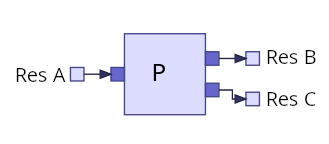
\includegraphics[scale=0.5]{img/node_port_graph.png}
  \caption{Port graph \isa{Primitive\ \isapars{Res\ A}\ \isapars{Res\ B\ \isasymodot\ Res\ C}\ \isaString{P}\ \isapars{}}}
  \label{fig:primitive_port_graph}
\end{figure}

For the sequential and parallel composition cases, we make use of the port graph sequencing (see Section~\ref{sec:port_graphs/mech/seq}) and juxtaposition (see Section~\ref{sec:port_graphs/mech/par}) respectively.
We first recursively construct the port graphs of the child processes and qualify them with distinct name atoms to prevent an overlap in the names they contain.
Then we apply the relevant operation to the resulting port graphs, which takes care of all other aspects given disjoint port graphs.
Instances for two primitive actions composed in sequence and in parallel are shown in Figure~\ref{fig:seq_par_port_graph}.

\begin{figure}[htbp]
  \begin{subfigure}{0.45\textwidth}
    \centering
    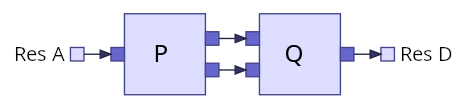
\includegraphics[scale=0.4]{img/seq_port_graph.png}
    \caption{Sequential composition}
    \label{fig:seq_port_graph}
  \end{subfigure}
  \begin{subfigure}{0.45\textwidth}
    \centering
    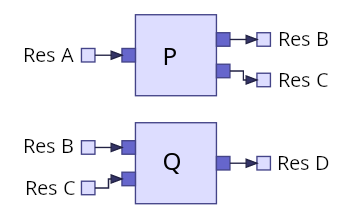
\includegraphics[scale=0.4]{img/par_port_graph.png}
    \caption{Parallel composition}
    \label{fig:par_port_graph}
  \end{subfigure}
  \caption{Process port graphs for sequential and parallel composition of primitive actions \isa{P:\ Res\ A\ \isasymrightarrow\ Res\ B\ \isasymodot\ Res\ C} and \isa{Q:\ Res\ B\ \isasymodot\ Res\ C\ \isasymrightarrow\ Res\ D}}
  \label{fig:seq_par_port_graph}
\end{figure}

For \isa{Identity} we build a port graph consisting of no node and a set of edges, one for each parallel part of the relevant resource going between two open ports, one input and one output.
We abstract this pattern in general port graphs for any list of data (in our case the parallel parts of a resource) and call it \isa{idPortGraph}.
Its instance for the three-atom resource \isa{Res\ A\ \isasymodot\ Res\ B\ \isasymodot\ Res\ C} is shown in Figure~\ref{fig:id_port_graph}.

\begin{figure}[htbp]
  \centering
  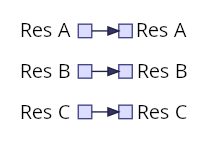
\includegraphics[scale=0.5]{img/id_port_graph.png}
  \caption{Process port graph for \isa{Identity\ \isapars{Res\ A\ \isasymodot\ Res\ B\ \isasymodot\ Res\ C}}}
  \label{fig:id_port_graph}
\end{figure}

For \isa{Swap} we build again a port graph consisting of no node and a set of edges, just like for \isa{Identity}, using parallel parts of the two resources being swapped.
But, in this case, we change the indices of the open output ports to reflect the swapped order of the resources.
We call the resulting pattern in general port graphs \isa{swapPortGraph}, parameterised by two lists of data for the ports.

Note that, during the layout step of visualising this port graph on its own, the different order stops being visually apparent due to the layout algorithm's goal of minimising edge crossings.
However, as shown in Figure~\ref{fig:swap_port_graph}, the reordering becomes apparent when we fix the port positions using primitive action nodes.

\begin{figure}[htbp]
  \centering
  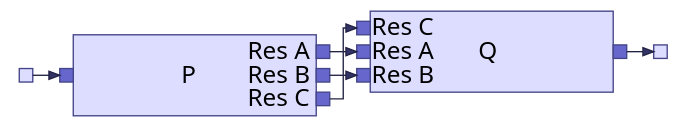
\includegraphics[scale=0.5]{img/swap_port_graph_alt.png}
  \caption{Process port graph involving \isa{Swap\ \isapars{Res\ A\ \isasymodot\ Res\ B}\ \isapars{Res\ C}}}
  \label{fig:swap_port_graph}
\end{figure}

For \isa{Duplicate} and \isa{Repeat} we use the same pattern: we build a port graph consisting of no node and one input port with two edges going from it to two output ports.
We call this pattern \isa{forkPortGraph}, parameterised by the single piece of data for all its open ports.
Its instance for duplicating a copyable atom \isa{data} is shown in Figure~\ref{fig:duplicate_port_graph}.

\begin{figure}[htbp]
  \centering
  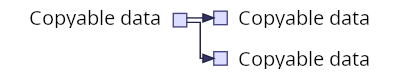
\includegraphics[scale=0.5]{img/duplicate_port_graph.png}
  \caption{Process port graph for \isa{Duplicate\ data}}
  \label{fig:duplicate_port_graph}
\end{figure}

For \isa{Erase} and \isa{Close} we use a very simple pattern: a single input port with no edges or output ports.
This represents closing off whatever output port this single input is composed with.
Its instance for erasing a copyable atom \isa{data} is shown in Figure~\ref{fig:erase_port_graph}.

\begin{figure}[htbp]
  \centering
  
\includegraphics[scale=0.5]{img/erase_port_graph.png}
  \caption{Process port graph for \isa{Erase\ data}}
  \label{fig:erase_port_graph}
\end{figure}

For \isa{Once} we use a pattern similar to \isa{Identity} but, because of how its input and output interact with \isa{parallel{\isacharunderscore}parts}, there is only one edge.
Moreover, the origin and destination of that edge carry different resources as data: the origin carries a \isa{Repeatable} resource while the destination carries the corresponding \isa{Executable} resource.
Note that this is the first port graph pattern we use in which the labels on origin and destination of an edge differ.
Its instance for a repeatable process from \isa{\isafv{x}} to \isa{\isafv{y}} is shown in Figure~\ref{fig:erase_port_graph}.

\begin{figure}[htbp]
  \centering
  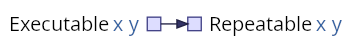
\includegraphics[scale=0.5]{img/once_port_graph.png}
  \caption{Process port graph for \isa{Once\ \isafv{x}\ \isafv{y}}}
  \label{fig:once_port_graph}
\end{figure}

For \isa{Forget} we build a port graph consisting of no node, a number of input ports and a single output port, and edges from every input to the sole output.
We use parallel parts of the input resource to label the input ports and the output \isa{Anything} resource to label the output port.
This represents any complex resource merging into a single \isa{Anything} resource, forgetting any details about it including that it may have consisted of multiple parts.
Note that in this port graph we also may have edges with origin and destination labelled differently.
Its instance for the resources \isa{Res\ A}, \isa{Res\ B} and \isa{Res\ C} is shown in Figure~\ref{fig:forget_port_graph}.

\begin{figure}[htbp]
  \centering
  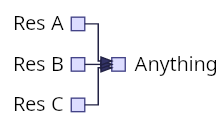
\includegraphics[scale=0.5]{img/forget_port_graph.png}
  \caption{Process port graph for \isa{Forget {Res\ A\ \isasymodot\ Res\ B}\ \isasymodot\ Res\ C}}
  \label{fig:forget_port_graph}
\end{figure}

This concludes the patterns we use to generate port graphs from process compositions.
Figure~\ref{fig:fourGears_port_graph} illustrates the port graph construction on a more complex process composition, the manufacturing of four iron gears per second defined in Section~\ref{sec:cases/factorio/gears}.
We next turn to the properties that our process port graphs satisfy.

\begin{figure}[htbp]
  \centering
  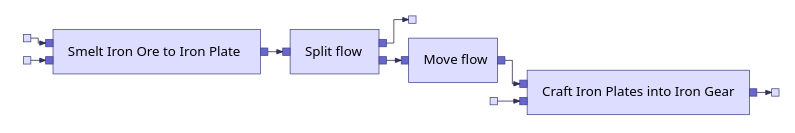
\includegraphics[scale=0.5]{img/fourGears_port_graph.png}
  \caption{Process port graph for manufacturing four iron gears per second (see Section~\ref{sec:cases/factorio/gears} for details of this process). We omit open port labels due to their size.}
  \label{fig:fourGears_port_graph}
\end{figure}

\subsection{Properties of Process Port Graphs}
\label{sec:port_graphs/process/prop}

Before we discuss specific properties, recall that our process port graph construction is not defined for processes that make use of non-deterministic or higher-order features.
\cbstart
To exclude such processes from consideration, we define the predicate \isa{pgDefined} (see Appendix~\ref{app:pgDefined} for its full definition).
We then assume that any process used in \isa{pgConstruct} satisfies this condition.
\cbend

We start our verification by proving that our construction, given a composition it is fully defined on, results in a well-formed port graph with flow.
Proving that each of the port graph patterns we use is well-formed and satisfies the flow requirements is quite simple, because having concrete port graphs simplifies much of the quantification in the locale assumptions.
The cases for parallel and sequential composition are simple, because we prove that both port graph juxtaposition and sequencing satisfy the \isa{port{\isacharunderscore}graph{\isacharunderscore}flow} locale just after defining them (Lemma~\ref{isa:port_graph_juxtapose} and Lemma~\ref{isa:port_graph_flow_seqPortGraphs}).
Therefore we now only need to prove that qualifying the child port graphs with distinct atoms (\isa{SeqL} and \isa{SeqR}, or \isa{ParL} and \isa{ParR}) indeed makes them disjoint, which is easily done.
As a result, we have the following theorem in Isabelle/HOL:
\begin{isalemma}[Process port graphs are well-formed]{isa:port_graph_flow_pgConstruct}
  \isacomm{lemma}\isamarkupfalse%
\ port{\isacharunderscore}graph{\isacharunderscore}flow{\isacharunderscore}pgConstruct{\isacharcolon}\isanewline
\ \ \isaOcomm{assumes}\ {\isachardoublequoteopen}pgDefined\ \isafv{x}{\isachardoublequoteclose}\isanewline
\ \ \ \ \ \ \isaOcomm{shows}\ {\isachardoublequoteopen}port{\isacharunderscore}graph{\isacharunderscore}flow\ {\isacharparenleft}pgConstruct\ \isafv{x}{\isacharparenright}{\isachardoublequoteclose}

\end{isalemma}

Then we show that the open ports of the constructed port graph correspond to parallel parts (given in Definition~\ref{isa:parallel_parts}) of the process composition's input and output resources:
\begin{isalemma}[Open ports correspond to input and output]{isa:pgConstruct_ports}
  \isacomm{lemma}\isamarkupfalse%
\ pgConstruct{\isacharunderscore}ports{\isacharcolon}\isanewline
\ \ \isaOcomm{assumes}\ {\isachardoublequoteopen}pgDefined\ \isafv{x}{\isachardoublequoteclose}\isanewline
\ \ \ \ \ \ \isaOcomm{shows}\ {\isachardoublequoteopen}set\ {\isacharparenleft}pg{\isacharunderscore}ports\ {\isacharparenleft}pgConstruct\ \isafv{x}{\isacharparenright}{\isacharparenright}\ {\isacharequal}\isanewline
\isaindent{\ \ \ \ \ \ \isaOcomm{shows}\ {\isachardoublequoteopen}}set\ {\isacharparenleft}parallelPorts\ {\isadigit{0}}\ In\ {\isacharparenleft}input\ \isafv{x}{\isacharparenright}\ {\isacharat}\ parallelPorts\ {\isadigit{0}}\ Out\ {\isacharparenleft}output\ \isafv{x}{\isacharparenright}{\isacharparenright}{\isachardoublequoteclose}

\end{isalemma}

Moreover, the nodes of the port graph also correspond to the primitive actions present in the process composition.
To prove this, we define the function \isa{namedPrimitives} that operates exactly as the function \isa{primitives} (see Section~\ref{sec:proc/type/primitive}) but also collects the path to each primitive action.
We show that the path is the node name, the action's label and metadata are the node label, and the action's input and output form the node ports:
\begin{isalemma}[Nodes correspond to primitive actions]{isa:pgConstruct_nodes}
  \isacomm{lemma}\ pgConstruct{\isacharunderscore}nodes{\isacharcolon}\isanewline
\ \ \isaOcomm{assumes}\ {\isachardoublequoteopen}pgDefined\ \isafv{x}{\isachardoublequoteclose}\isanewline
\ \ \ \ \ \ \isaOcomm{shows}\ pg{\isacharunderscore}nodes\ {\isacharparenleft}pgConstruct\ \isafv{x}{\isacharparenright}\ {\isacharequal}\isanewline
\isaindent{\ \ \ \ \ \ \isaOcomm{shows}\ }map\ {\isacharparenleft}{\isasymlambda}{\isacharparenleft}\isabv{n}{\isacharcomma}\ \isabv{ins}{\isacharcomma}\ \isabv{outs}{\isacharcomma}\ \isabv{l}{\isacharcomma}\ \isabv{m}{\isacharparenright}{\isachardot}\isanewline
\isaindent{\ \ \ \ \ \ \isaOcomm{shows}\ map\ {\isacharparenleft}{\isasymlambda}}Node\ \isabv{n}\ {\isacharparenleft}NodePrimitive\ \isabv{l\ m}{\isacharparenright}\ {\isacharparenleft}parallelPorts\ {\isadigit{0}}\ In\ \isabv{ins}\ {\isacharat}\isanewline
\isaindent{\ \ \ \ \ \ \isaOcomm{shows}\ map\ {\isacharparenleft}{\isasymlambda}Node\ \isabv{n}\ {\isacharparenleft}NodePrimitive\ \isabv{l\ m}{\isacharparenright}\ {\isacharparenleft}}parallelPorts\ {\isadigit{0}}\ Out\ \isabv{outs}{\isacharparenright}{\isacharparenright}\isanewline
\isaindent{\ \ \ \ \ \ \isaOcomm{shows}\ map\ }{\isacharparenleft}namedPrimitives\ \isafv{x}{\isacharparenright}{\isachardoublequoteclose}

\end{isalemma}

The remainder of the properties we highlight in this section concern situations where different process compositions yield equivalent port graphs.
These capture a deeper aspect of process compositions than the surface-level syntax: they say that two compositions, although syntactically different, represent the same structure of connections between actions.
In Section~\ref{sec:port_graphs/conc} we discuss future work taking further advantage of this aspect of the equivalence.

To start with, we can show that, up to equivalence of constructed port graphs, the identity process behaves as unit for both sequential and parallel composition:
\begin{isalemma}[Identity process is sequential unit]{isa:pgConstruct_seq_unit_pgEquiv}
  \isacomm{lemma}\ pgConstruct{\isacharunderscore}seq{\isacharunderscore}unit{\isacharunderscore}pgEquiv{\isacharcolon}\isanewline
\ \ \isaOcomm{assumes}\ {\isachardoublequoteopen}pgDefined\ \isafv{x}{\isachardoublequoteclose}\isanewline
\ \ \ \ \ \ \isaOcomm{shows}\ {\isachardoublequoteopen}pgConstruct\ {\isacharparenleft}Seq\ {\isacharparenleft}Identity\ {\isacharparenleft}input\ \isafv{x}{\isacharparenright}{\isacharparenright}\ \isafv{x}{\isacharparenright}\ {\isasymapprox}\ pgConstruct\ \isafv{x}{\isachardoublequoteclose}\isanewline
\ \ \ \ \ \ \ \ \ \ \isaOcomm{and}\ {\isachardoublequoteopen}pgConstruct\ {\isacharparenleft}Seq\ \isafv{x}\ {\isacharparenleft}Identity\ {\isacharparenleft}output\ \isafv{x}{\isacharparenright}{\isacharparenright}{\isacharparenright}\ {\isasymapprox}\ pgConstruct\ \isafv{x}{\isachardoublequoteclose}

\end{isalemma}
\pagebreak
\begin{isalemma}[Identity process is parallel unit]{isa:pgConstruct_par_unit_pgEquiv}
  \isacomm{lemma}\ pgConstruct{\isacharunderscore}par{\isacharunderscore}unit{\isacharunderscore}pgEquiv{\isacharcolon}\isanewline
\ \ \isaOcomm{assumes}\ {\isachardoublequoteopen}pgDefined\ \isafv{x}{\isachardoublequoteclose}\isanewline
\ \ \ \ \ \ \isaOcomm{shows}\ {\isachardoublequoteopen}pgConstruct\ {\isacharparenleft}Par\ {\isacharparenleft}Identity\ Empty{\isacharparenright}\ \isafv{x}{\isacharparenright}\ {\isasymapprox}\ pgConstruct\ \isafv{x}{\isachardoublequoteclose}\isanewline
\ \ \ \ \ \ \ \ \ \ \isaOcomm{and}\ {\isachardoublequoteopen}pgConstruct\ {\isacharparenleft}Par\ \isafv{x}\ {\isacharparenleft}Identity\ Empty{\isacharparenright}{\isacharparenright}\ {\isasymapprox}\ pgConstruct\ \isafv{x}{\isachardoublequoteclose}

\end{isalemma}

We can also take the theorems about when port graph sequencing and juxtaposition are associative and show that the process port graphs satisfy their assumptions.
This is because qualifying port graphs with distinct name atoms makes them disjoint while being equivalent to the original.
As a result, we get the following two theorems:
\begin{isalemma}[Parallel and sequential composition are associative]{isa:pgConstruct_assoc}
  \isacomm{lemma}\isanewline
\ \ \isaOcomm{assumes}\ {\isachardoublequoteopen}pgDefined\ \isafv{x}{\isachardoublequoteclose}\ \isaOcomm{and}\ {\isachardoublequoteopen}pgDefined\ \isafv{y}{\isachardoublequoteclose}\ \isaOcomm{and}\ {\isachardoublequoteopen}pgDefined\ \isafv{z}{\isachardoublequoteclose}\isanewline
\ \ \ \ \ \ \isaOcomm{shows}\ pgConstruct{\isacharunderscore}Par{\isacharunderscore}assoc{\isacharcolon}\isanewline
\isaindent{\ \ \ \ \ \ \isaOcomm{shows}\ }{\isachardoublequoteopen}pgConstruct\ {\isacharparenleft}Par\ {\isacharparenleft}Par\ \isafv{x\ y}{\isacharparenright}\ \isafv{z}{\isacharparenright}\ {\isasymapprox}\ pgConstruct\ {\isacharparenleft}Par\ \isafv{x}\ {\isacharparenleft}Par\ \isafv{y\ z}{\isacharparenright}{\isacharparenright}{\isachardoublequoteclose}\isanewline
\ \ \ \ \ \ \ \ \ \ \isaOcomm{and}\ pgConstruct{\isacharunderscore}Seq{\isacharunderscore}assoc{\isacharcolon}\isanewline
\isaindent{\ \ \ \ \ \ \ \ \ \ \isaOcomm{and}\ }{\isachardoublequoteopen}pgConstruct\ {\isacharparenleft}Seq\ {\isacharparenleft}Seq\ \isafv{x\ y}{\isacharparenright}\ \isafv{z}{\isacharparenright}\ {\isasymapprox}\ pgConstruct\ {\isacharparenleft}Seq\ \isafv{x}\ {\isacharparenleft}Seq\ \isafv{y\ z}{\isacharparenright}{\isacharparenright}{\isachardoublequoteclose}

\end{isalemma}

And we can show that the \isa{Duplicate} action forms a monoid in this way with the \isa{Erase} action as unit: erasing either result of duplication is as if we did nothing, and nesting duplications is associative.
Because the corresponding port graphs have no nodes that would require renaming, the relations can be shown as \emph{equalities} of port graphs instead of just equivalences.
All three statements are as follows:
\begin{isalemma}[\isa{Duplicate} and \isa{Erase} form a monoid]{isa:pgConstruct_duplicate_erase}
  \isacomm{lemma}\isamarkupfalse%
\isanewline
\ \ \isaOcomm{shows}\ pgConstruct{\isacharunderscore}duplicate{\isacharunderscore}eraseL{\isacharcolon}\isanewline
\ \ \ \ pgConstruct\ {\isacharparenleft}Seq\ {\isacharparenleft}Duplicate\ \isafv{x}{\isacharparenright}\ {\isacharparenleft}Par\ {\isacharparenleft}Erase\ \isafv{x}{\isacharparenright}\ {\isacharparenleft}Identity\ {\isacharparenleft}Copyable\ \isafv{x}{\isacharparenright}{\isacharparenright}{\isacharparenright}{\isacharparenright}\ {\isacharequal}\isanewline
\ \ \ \ pgConstruct\ {\isacharparenleft}Identity\ {\isacharparenleft}Copyable\ \isafv{x}{\isacharparenright}{\isacharparenright}{\isachardoublequoteclose}\isanewline
\ \ \ \ \ \ \isaOcomm{and}\ pgConstruct{\isacharunderscore}duplicate{\isacharunderscore}eraseR{\isacharcolon}\isanewline
\ \ \ \ pgConstruct\ {\isacharparenleft}Seq\ {\isacharparenleft}Duplicate\ \isafv{x}{\isacharparenright}\ {\isacharparenleft}Par\ {\isacharparenleft}Identity\ {\isacharparenleft}Copyable\ \isafv{x}{\isacharparenright}{\isacharparenright}\ {\isacharparenleft}Erase\ \isafv{x}{\isacharparenright}{\isacharparenright}{\isacharparenright}\ {\isacharequal}\isanewline
\ \ \ \ pgConstruct\ {\isacharparenleft}Identity\ {\isacharparenleft}Copyable\ \isafv{x}{\isacharparenright}{\isacharparenright}{\isachardoublequoteclose}\isanewline
\ \ \ \ \ \ \isaOcomm{and}\ pgConstruct{\isacharunderscore}duplicate{\isacharunderscore}assoc{\isacharcolon}\isanewline
\ \ \ \ pgConstruct\ {\isacharparenleft}Seq\ {\isacharparenleft}Duplicate\ \isafv{x}{\isacharparenright}\ {\isacharparenleft}Par\ {\isacharparenleft}Identity\ {\isacharparenleft}Copyable\ \isafv{x}{\isacharparenright}{\isacharparenright}\ {\isacharparenleft}Duplicate\ \isafv{x}{\isacharparenright}{\isacharparenright}{\isacharparenright}\ {\isacharequal}\isanewline
\ \ \ \ pgConstruct\ {\isacharparenleft}Seq\ {\isacharparenleft}Duplicate\ \isafv{x}{\isacharparenright}\ {\isacharparenleft}Par\ {\isacharparenleft}Duplicate\ \isafv{x}{\isacharparenright}\ {\isacharparenleft}Identity\ {\isacharparenleft}Copyable\ \isafv{x}{\isacharparenright}{\isacharparenright}{\isacharparenright}{\isacharparenright}{\isachardoublequoteclose}

\end{isalemma}

Increasing the statement complexity, we can prove {\cbstart}that any process that composes like an identity action produces a port graph equivalent to it.
More precisely, by composing like an identity action we mean that
\begin{enumerate*}[label=(\roman*)]
  \item sequential composition of the candidate process with itself is valid, and
  \item for any other process whose sequential composition with the candidate is valid the result produces a port graph equivalent to that other process.
\end{enumerate*}
This yields two theorems, Lemma~\ref{isa:pgConstruct_ide_input} and Lemma~\ref{isa:pgConstruct_ide_output}, which differ in the ordering of the sequential composition and thus in the identity action using the input or output resource.
\cbend

\begin{isalemma}[Left unit of \isa{Seq} is equivalent to an identity on input]{isa:pgConstruct_ide_input}
  \isacomm{lemma}\isamarkupfalse%
\ pgConstruct{\isacharunderscore}ide{\isacharunderscore}input{\isacharcolon}\isanewline
\ \ \isaOcomm{assumes}\ {\isachardoublequoteopen}pgDefined\ \isafv{x}{\isachardoublequoteclose}\isanewline
\ \ \ \ \ \ \ \ \ \ \isaOcomm{and}\ {\isachardoublequoteopen}valid\ {\isacharparenleft}Seq\ \isafv{x\ x}{\isacharparenright}{\isachardoublequoteclose}\isanewline
\ \ \ \ \ \ \ \ \ \ \isaOcomm{and}\ {\isachardoublequoteopen}{\isasymAnd}\isabv{f}{\isachardot}\ {\isasymlbrakk}pgDefined\ \isabv{f}{\isacharsemicolon}\ valid\ {\isacharparenleft}Seq\ \isabv{f}\ \isafv{x}{\isacharparenright}{\isasymrbrakk}\isanewline
\isaindent{\ \ \ \ \ \ \ \ \ \ \isaOcomm{and}\ {\isachardoublequoteopen}{\isasymAnd}\isabv{f}{\isachardot}\ }{\isasymLongrightarrow}\ pgConstruct\ {\isacharparenleft}Seq\ \isabv{f}\ \isafv{x}{\isacharparenright}\ {\isasymapprox}\ pgConstruct\ \isabv{f}{\isachardoublequoteclose}\isanewline
\ \ \ \ \ \ \isaOcomm{shows}\ {\isachardoublequoteopen}pgConstruct\ \isafv{x}\ {\isasymapprox}\ pgConstruct\ {\isacharparenleft}Identity\ {\isacharparenleft}input\ \isafv{x}{\isacharparenright}{\isacharparenright}{\isachardoublequoteclose}

\end{isalemma}
\begin{isalemma}[Right unit of \isa{Seq} is equivalent to an identity on output]{isa:pgConstruct_ide_output}
  \isacomm{lemma}\isamarkupfalse%
\ pgConstruct{\isacharunderscore}ide{\isacharunderscore}output{\isacharcolon}\isanewline
\ \ \isaOcomm{assumes}\ {\isachardoublequoteopen}pgDefined\ \isafv{x}{\isachardoublequoteclose}\isanewline
\ \ \ \ \ \ \ \ \ \ \isaOcomm{and}\ {\isachardoublequoteopen}valid\ {\isacharparenleft}Seq\ \isafv{x\ x}{\isacharparenright}{\isachardoublequoteclose}\isanewline
\ \ \ \ \ \ \ \ \ \ \isaOcomm{and}\ {\isachardoublequoteopen}{\isasymAnd}\isabv{f}{\isachardot}\ {\isasymlbrakk}pgDefined\ \isabv{f}{\isacharsemicolon}\ valid\ {\isacharparenleft}Seq\ \isafv{x}\ \isabv{f}{\isacharparenright}{\isasymrbrakk}\isanewline
\isaindent{\ \ \ \ \ \ \ \ \ \ \isaOcomm{and}\ {\isachardoublequoteopen}{\isasymAnd}\isabv{f}{\isachardot}\ }{\isasymLongrightarrow}\ pgConstruct\ {\isacharparenleft}Seq\ \isafv{x}\ \isabv{f}{\isacharparenright}\ {\isasymapprox}\ pgConstruct\ \isabv{f}{\isachardoublequoteclose}\isanewline
\ \ \ \ \ \ \isaOcomm{shows}\ {\isachardoublequoteopen}pgConstruct\ \isafv{x}\ {\isasymapprox}\ pgConstruct\ {\isacharparenleft}Identity\ {\isacharparenleft}output\ \isafv{x}{\isacharparenright}{\isacharparenright}{\isachardoublequoteclose}

\end{isalemma}

In the following two sections we turn to two statements about processes that this new graphical perspective allows us to prove.
One describes when parallel and sequential composition of processes can pass through each other without affecting the connections between actions.
The other characterises the range of connections that can occur in valid process compositions, serving as a graphical counterpart to our demonstration of linearity in Chapter~\ref{ch:linearity}.

\section{Process Interchange}
\label{sec:port_graphs/interchange}

In general, parallel and sequential composition of processes do not distribute over each other.
(For a more thorough discussion of behaviour one expects from concurrent programs and process calculi, see Hoare and van~Staden~\cite{hoare_staden-2014}.)
In our notation, this means we would expect \isa{Seq\ \isapars{Par\ \isafv{R\ S}}\ \isapars{Par\ \isafv{T\ U}}} to have more constrained behaviour than \isa{Par\ \isapars{Seq\ \isafv{R\ T}}\ \isapars{Seq\ \isafv{S\ U}}} (when they are both valid compositions).
This is because, in a direct reading, the latter form allows for more interleaving of the processes: the former stipulates that we do \isa{\isafv{R}} and\ \isa{\isafv{S}} before \isa{\isafv{T}} and\ \isa{\isafv{U}}, while the latter allows us to do \isa{\isafv{T}} before \isa{\isafv{S}} as long as it follows \isa{\isafv{R}}.
In practice, this may for instance be the case if \isa{\isafv{U}} depends on \isa{\isafv{R}} in order to execute.

However, for both forms to be valid in our framework we must have \isa{output\ \isafv{R}\ \isacharequal\ input\ \isafv{T}} and \isa{output\ \isafv{S}\ \isacharequal\ input\ \isafv{U}}.
Note that this means there is no resource passing from \isa{\isafv{R}} to \isa{\isafv{U}} and from \isa{\isafv{S}} to \isa{\isafv{T}}.
And, because resources in our framework model dependency between actions, we would expect to be able to do \isa{\isafv{T}} without first doing \isa{\isafv{S}}.
Because through resources in our framework we have this extra information about the dependency between actions, we would like to equate the two forms when both are valid.

We cannot equate the two forms in themselves, because they are different compositions of processes.
But, because our claim about their close relation is based in connections, we can relate them through the port graphs they generate.
A simple indication of this is that, when \cbar{both} compositions are valid, our implementation of process diagrams (see Section~\ref{sec:proc/diag}) draws the same diagram for both, shown in Figure~\ref{fig:interchange-diag}.

\begin{figure}[hbtp]
  \centering
  \includesvg[scale=1]{img-gen/interchange.svg}
  \caption{Common process diagram for the compositions \isa{Seq\ \isapars{Par\ \isafv{R\ S}}\ \isapars{Par\ \isafv{T\ U}}} and \isa{Par\ \isapars{Seq\ \isafv{R\ T}}\ \isapars{Seq\ \isafv{S\ U}}}}
  \label{fig:interchange-diag}
\end{figure}

With our process port graphs, we can make this relation fully formal: for any four processes, if both the composition forms are valid then the port graphs resulting from them are equivalent.
Note that validity of one subsumes validity of the other, so we need only assume one is valid.
That is, in Isabelle/HOL:
\begin{isalemma}[Interchange of process port graphs]{isa:pgConstruct_interchange}
  \isacomm{lemma}\ pgConstruct{\isacharunderscore}interchange{\isacharcolon}\isanewline
\ \ \isaOcomm{assumes}\ {\isachardoublequoteopen}pgDefined\ \isafv{r}{\isachardoublequoteclose}\ \isaOcomm{and}\ {\isachardoublequoteopen}pgDefined\ \isafv{t}{\isachardoublequoteclose}\ \isaOcomm{and}\ {\isachardoublequoteopen}pgDefined\ \isafv{s}{\isachardoublequoteclose}\ \isaOcomm{and}\ {\isachardoublequoteopen}pgDefined\ \isafv{u}{\isachardoublequoteclose}\isanewline
\ \ \ \ \ \ \ \ \ \ \isaOcomm{and}\ {\isachardoublequoteopen}valid\ {\isacharparenleft}Par\ {\isacharparenleft}Seq\ \isafv{r\ t}{\isacharparenright}\ {\isacharparenleft}Seq\ \isafv{s\ u}{\isacharparenright}{\isacharparenright}{\isachardoublequoteclose}\isanewline
\ \ \ \ \ \ \isaOcomm{shows}\ {\isachardoublequoteopen}pgConstruct\ {\isacharparenleft}Seq\ {\isacharparenleft}Par\ \isafv{r\ s}{\isacharparenright}\ {\isacharparenleft}Par\ \isafv{t\ u}{\isacharparenright}{\isacharparenright}\ {\isasymapprox}\isanewline
\isaindent{\ \ \ \ \ \ \isaOcomm{shows}\ {\isachardoublequoteopen}}pgConstruct\ {\isacharparenleft}Par\ {\isacharparenleft}Seq\ \isafv{r\ t}{\isacharparenright}\ {\isacharparenleft}Seq\ \isafv{s\ u}{\isacharparenright}{\isacharparenright}{\isachardoublequoteclose}

\end{isalemma}

We prove this fact first as a general theorem about port graphs and then show that process port graphs satisfy its assumptions.
In that, we again use the fact that port graph qualification done as part of the construction makes the child port graphs disjoint while keeping them equivalent to the originals, and that process port graphs only use the input and output sides for ports.
Beyond all the parameters being well-formed port graphs with flow that are disjoint from each other, there are two interesting assumptions we need to satisfy.
They require that the number of output ports of \isa{pgConstruct\ \isafv{r}} must be equal to the number of input ports of \isa{pgConstruct\ \isafv{t}}, and the same for \isa{\isafv{s}} and \isa{\isafv{u}} respectively.
We prove these for process port graphs from the validity assumption and the fact that open ports of process port graphs correspond to the inputs and outputs of the relevant process.

As a result, while the two compositions are syntactically distinct and in the general context of concurrent process modelling we would not expect them to be the same, we can use the extra information expressed by resources in our framework and our connection to port graphs to prove when they result in the same connections between actions.
Figure~\ref{fig:interchange_port_graph} visualises the port graph that results from both forms, which, as expected, matches the unformalised process diagram in Figure~\ref{fig:interchange-diag}.

\begin{figure}[hbtp]
  \centering
  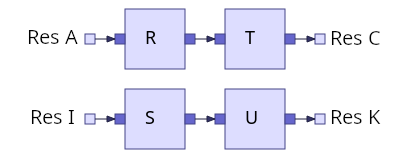
\includegraphics[scale=0.5]{img/interchange_port_graph.png}
  \caption{Port graph for both forms of nested parallel and sequential composition}
  \label{fig:interchange_port_graph}
\end{figure}

\section{Graphical Linearity}
\label{sec:port_graphs/linearity}

Our work in Chapter~\ref{ch:linearity} demonstrates process correctness, more specifically their linearity, by appealing to linear logic.
We transform all process compositions into deductions in linear logic while preserving their structure and then prove that for valid compositions the resulting deduction follows the rules of linear logic.

However, that demonstration does not say what linearity means directly in terms of the resources and processes, just that adherence to the rules of linear logic demonstrates it.
In this section we use our port graph construction to split all occurrences of resources in the process (represented by places of the constructed port graph) into five categories based on how they connect to other occurrences.
This characterises all the ways resources are manipulated in the process and allows us to then argue that they are being manipulated correctly by addressing each category.
\cbar{We first present the formal statement, followed by discussion of the cases it identifies.}

\pagebreak
\begin{isalemma}[Graphical linearity of process port graphs]{isa:pgConstruct_linearity}
  \isacomm{lemma}\ pgConstruct{\isacharunderscore}linearity{\isacharcolon}\isanewline
\ \ \isaOcomm{assumes}\ {\isachardoublequoteopen}pgDefined\ \isafv{x}{\isachardoublequoteclose}\ \isaOcomm{and}\ {\isachardoublequoteopen}valid\ \isafv{x}{\isachardoublequoteclose}\isanewline
\ \ \widthtoL{\isaOcomm{and}}{\isaOcomm{assumes}}\ {\isachardoublequoteopen}\isafv{p}\ {\isasymin}\ set\ {\isacharparenleft}pgraphPlaces\ {\isacharparenleft}pgConstruct\ \isafv{x}{\isacharparenright}{\isacharparenright}{\isachardoublequoteclose}\isanewline
\ \ \widthtoL{\isaOcomm{obtains}}{\isaOcomm{assumes}}\isanewline
\ \ \isaindent{\isacharbar\ }{\isacharparenleft}Linear{\isacharparenright}\isanewline
\ \ \isaindent{\isaOcomm{assumes}\ }{\isachardoublequoteopen}{\isasymnot}{\isacharparenleft}{\isasymexists}\isabv{a}{\isachardot}\ port{\isachardot}label\ {\isacharparenleft}place{\isacharunderscore}port\ \isafv{p}{\isacharparenright}\ {\isacharequal}\ Copyable\ \isabv{a}{\isacharparenright}{\isachardoublequoteclose}\isanewline
\ \ \widthtoL{\isaOcomm{and}}{\isaOcomm{assumes}}\ {\isachardoublequoteopen}{\isasymnot}{\isacharparenleft}{\isasymexists}\isabv{a\ b}{\isachardot}\ port{\isachardot}label\ {\isacharparenleft}place{\isacharunderscore}port\ \isafv{p}{\isacharparenright}\ {\isacharequal}\ Repeatable\ \isabv{a\ b}{\isacharparenright}{\isachardoublequoteclose}\isanewline
\ \ \widthtoL{\isaOcomm{and}}{\isaOcomm{assumes}}\ {\isachardoublequoteopen}port{\isachardot}label\ {\isacharparenleft}place{\isacharunderscore}port\ \isafv{p}{\isacharparenright}\ {\isasymnoteq}\ Anything{\isachardoublequoteclose}\isanewline
\ \ \widthtoL{\isaOcomm{and}}{\isaOcomm{assumes}}\ {\isachardoublequoteopen}{\isasymexists}{\isacharbang}\isabv{e}\ {\isasymin}\ set\ {\isacharparenleft}pg{\isacharunderscore}edges\ {\isacharparenleft}pgConstruct\ \isafv{x}{\isacharparenright}{\isacharparenright}{\isachardot}\ edge{\isacharunderscore}from\ \isabv{e}\ {\isacharequal}\ \isafv{p}\ {\isasymor}\ edge{\isacharunderscore}to\ \isabv{e}\ {\isacharequal}\ \isafv{p}{\isachardoublequoteclose}\isanewline
\ \ {\isacharbar}\ {\isacharparenleft}NonLinear{\isacharunderscore}Origin{\isacharparenright}\isanewline
\ \ \isaindent{\isaOcomm{assumes}\ }{\isachardoublequoteopen}{\isacharparenleft}{\isasymexists}\isabv{a}{\isachardot}\ port{\isachardot}label\ {\isacharparenleft}place{\isacharunderscore}port\ \isafv{p}{\isacharparenright}\ {\isacharequal}\ Copyable\ \isabv{a}{\isacharparenright}\ {\isasymor}\isanewline
\ \ \isaindent{\isaOcomm{assumes}\ }{\isacharparenleft}{\isasymexists}\isabv{a\ b}{\isachardot}\ port{\isachardot}label\ {\isacharparenleft}place{\isacharunderscore}port\ \isafv{p}{\isacharparenright}\ {\isacharequal}\ Repeatable\ \isabv{a\ b}{\isacharparenright}{\isachardoublequoteclose}\isanewline
\ \ \widthtoL{\isaOcomm{and}}{\isaOcomm{assumes}}\ {\isachardoublequoteopen}{\isasymnot}{\isacharparenleft}{\isasymexists}\isabv{e}\ {\isasymin}\ set\ {\isacharparenleft}pg{\isacharunderscore}edges\ {\isacharparenleft}pgConstruct\ \isafv{x}{\isacharparenright}{\isacharparenright}{\isachardot}\ edge{\isacharunderscore}to\ \isabv{e}\ {\isacharequal}\ \isafv{p}{\isacharparenright}{\isachardoublequoteclose}\isanewline
\ \ {\isacharbar}\ {\isacharparenleft}NonLinear{\isacharunderscore}Destin{\isacharparenright}\isanewline
\ \ \isaindent{\isaOcomm{assumes}\ }{\isachardoublequoteopen}{\isacharparenleft}{\isasymexists}\isabv{a}{\isachardot}\ port{\isachardot}label\ {\isacharparenleft}place{\isacharunderscore}port\ \isafv{p}{\isacharparenright}\ {\isacharequal}\ Copyable\ \isabv{a}{\isacharparenright}\ {\isasymor}\isanewline
\ \ \isaindent{\isaOcomm{assumes}\ }{\isacharparenleft}{\isasymexists}\isabv{a\ b}{\isachardot}\ port{\isachardot}label\ {\isacharparenleft}place{\isacharunderscore}port\ \isafv{p}{\isacharparenright}\ {\isacharequal}\ Repeatable\ \isabv{a\ b}{\isacharparenright}{\isachardoublequoteclose}\isanewline
\ \ \widthtoL{\isaOcomm{and}}{\isaOcomm{assumes}}\ {\isachardoublequoteopen}{\isasymnot}{\isacharparenleft}{\isasymexists}\isabv{e}\ {\isasymin}\ set\ {\isacharparenleft}pg{\isacharunderscore}edges\ {\isacharparenleft}pgConstruct\ \isafv{x}{\isacharparenright}{\isacharparenright}{\isachardot}\ edge{\isacharunderscore}from\ \isabv{e}\ {\isacharequal}\ \isafv{p}{\isacharparenright}{\isachardoublequoteclose}\isanewline
\ \ \widthtoL{\isaOcomm{and}}{\isaOcomm{assumes}}\ {\isachardoublequoteopen}{\isasymexists}{\isacharbang}\isabv{e}\ {\isasymin}\ set\ {\isacharparenleft}pg{\isacharunderscore}edges\ {\isacharparenleft}pgConstruct\ \isafv{x}{\isacharparenright}{\isacharparenright}{\isachardot}\ edge{\isacharunderscore}to\ \isabv{e}\ {\isacharequal}\ \isafv{p}{\isachardoublequoteclose}\isanewline
\ \ {\isacharbar}\ {\isacharparenleft}Anything{\isacharunderscore}Origin{\isacharparenright}\isanewline
\ \ \isaindent{\isaOcomm{assumes}\ }{\isachardoublequoteopen}port{\isachardot}label\ {\isacharparenleft}place{\isacharunderscore}port\ \isafv{p}{\isacharparenright}\ {\isacharequal}\ Anything{\isachardoublequoteclose}\isanewline
\ \ \widthtoL{\isaOcomm{and}}{\isaOcomm{assumes}}\ {\isachardoublequoteopen}{\isasymexists}{\isacharbang}\isabv{e}\ {\isasymin}\ set\ {\isacharparenleft}pg{\isacharunderscore}edges\ {\isacharparenleft}pgConstruct\ \isafv{x}{\isacharparenright}{\isacharparenright}{\isachardot}\ edge{\isacharunderscore}from\ \isabv{e}\ {\isacharequal}\ \isafv{p}{\isachardoublequoteclose}\isanewline
\ \ \widthtoL{\isaOcomm{and}}{\isaOcomm{assumes}}\ {\isachardoublequoteopen}{\isasymnot}{\isacharparenleft}{\isasymexists}\isabv{e}\ {\isasymin}\ set\ {\isacharparenleft}pg{\isacharunderscore}edges\ {\isacharparenleft}pgConstruct\ \isafv{x}{\isacharparenright}{\isacharparenright}{\isachardot}\ edge{\isacharunderscore}to\ \isabv{e}\ {\isacharequal}\ \isafv{p}{\isacharparenright}{\isachardoublequoteclose}\isanewline
\ \ {\isacharbar}\ {\isacharparenleft}Anything{\isacharunderscore}Destin{\isacharparenright}\isanewline
\ \ \isaindent{\isaOcomm{assumes}\ }{\isachardoublequoteopen}port{\isachardot}label\ {\isacharparenleft}place{\isacharunderscore}port\ \isafv{p}{\isacharparenright}\ {\isacharequal}\ Anything{\isachardoublequoteclose}\isanewline
\ \ \widthtoL{\isaOcomm{and}}{\isaOcomm{assumes}}\ {\isachardoublequoteopen}{\isasymnot}{\isacharparenleft}{\isasymexists}\isabv{e}\ {\isasymin}\ set\ {\isacharparenleft}pg{\isacharunderscore}edges\ {\isacharparenleft}pgConstruct\ \isafv{x}{\isacharparenright}{\isacharparenright}{\isachardot}\ edge{\isacharunderscore}from\ \isabv{e}\ {\isacharequal}\ \isafv{p}{\isacharparenright}{\isachardoublequoteclose}

\end{isalemma}

\cbstart
As with other properties of process port graphs up to this point, we start by assuming that the process \isa{\isafv{x}} in question has no non-deterministic or higher-order features.
Additionally, we assume that it is valid.
While that is not always needed for the resulting port graph to have certain properties (such as Lemma~\ref{isa:pgConstruct_ports}), it is vital in this case.
Then we fix a place \isa{\isafv{p}} in the port graph constructed from \isa{\isafv{x}} and prove that each such place falls into one of five cases:
\cbend
\begin{itemize}
  \item It is labelled with a linear resource and there is a unique edge incident on it, or
  \item It carries a copyable or repeatable resource (\isa{Copyable} or \isa{Repeatable}) and:
    \begin{itemize}
      \item there is no edge coming into it but an arbitrary number of edges coming from it, or
      \item there is no edge coming from it but there is a unique edge coming into it; or
    \end{itemize}
  \item It carries the \isa{Anything} resource and:
    \begin{itemize}
      \item there is a unique edge coming from it but no edge coming into it, or
      \item there is a no edge coming from it but an arbitrary number of edges coming into it.
    \end{itemize}
\end{itemize}

The proof of this theorem consists of six major sub-lemmas totalling around 2500 lines of Isabelle script.
Each proceeds by induction on the process composition structure, and case analysis covering the possible resource labels and incident edges.
In each case we simplify the port graph construction and arrive either at a pattern fitting one of the above five cases or a contradiction, meaning that incompatible pattern cannot arise by constructing a port graph from a valid process composition.

One crucial fact used in this proof is that all edges in the port graph construction have the same resource label on their origin and their destination, except for those turning a \isa{Repeatable} resource into an \isa{Executable} resource or any resource into the \isa{Anything} resource.
This allows us to prove that our goal property is preserved through sequencing of port graphs.

Let us now discuss in more detail the five cases into which this theorem splits connections in process port graphs, along with what they mean for the resources involved.

The first case is the most important: every linear resource (i.e.\ not copyable, repeatable or \isa{Anything}) is moved from exactly one origin to exactly one destination.
As a result, no linear resource is left where it is produced or used to satisfy multiple requirements, and every action requiring a linear resource has a unique source for it.

The remaining cases characterise the allowed exceptions to the first case.
The second and third cases say that copyable and repeatable resources can link to any number of destinations but must still have a unique origin.
That is, they can be copied and erased, but not merged.

The fourth and fifth cases say that the \isa{Anything} resource can be made by merging any number of other resources but after formation must be treated linearly.
This represents the idea of \isa{Anything} as grouping together arbitrary resources and treating them as one homogeneous object, which is then still a resource and must be treated as such.

With reference to our use of linear logic for similar purposes in Chapter~\ref{ch:linearity}, the first case corresponds to the base way how linear logic manipulates propositions, while the second and third cases correspond to the extra allowances for the \isa{\isacharbang} modality and the fourth and fifth cases correspond to the extra allowances of the \isa{\isasymbottom} proposition.
However, here we are explicitly using the language of connections between nodes which represent primitive actions.

Note that, because our present port graph construction does not cover all process compositions, this does not supersede the demonstration through linear logic.
Nevertheless, it offers a valuable perspective on the same high-level issue of process composition correctness and shows that our graphical approach detailed in this chapter can be fruitfully applied to verifying process models.

\section{Port Graph Transition System}
\label{sec:port_graphs/trans}

So far this chapter, we have been using port graphs to represent the structure of a process composition in a way inspired by the process diagrams of Section~\ref{sec:proc/diag}.
We can, however, form an additional relationship between port graphs and processes: behaviour, expressed as a transition system.
In this section we describe a transition system on port graphs, which in turn induces a transition system on process compositions through the port graphs constructed from them.
That in turn allows us to better formalise the meaning of different process compositions.

The intuition behind the port graph transition system relies on viewing nodes as actions and edges as dependencies between them, just as we do with process port graphs.
To make a transition, we find a node that has no incoming edge from another node.
This represents its lack of dependency on any other node.
Then we remove that node and all its adjacent edges from the port graph, which represents performing that action and distributing its results.
In the absence of dependency loops, this will either result in another transition candidate or a port graph with no more nodes.

In our mechanisation of this idea, we start by defining the \emph{node flow}.
This relation orders nodes based on the edges going between them, placing one node before another node if there is an edge from a port of the former to a port of the latter.
In Isabelle/HOL we define this as an inductive relation:
\begin{isadef}[Node flow]{isa:node_flow}
  \isacomm{inductive}\ node{\isacharunderscore}flow\ {\isacharcolon}{\isacharcolon}\ {\isachardoublequoteopen}{\isacharparenleft}\isatv{s}{\isacharcomma}\ \isatv{a}{\isacharcomma}\ \isatv{p}{\isacharcomma}\ \isatv{l}{\isacharparenright}\ port{\isacharunderscore}graph\isanewline
\isaindent{\isacomm{inductive}\ node{\isacharunderscore}flow\ }{\isasymRightarrow}\ {\isacharparenleft}\isatv{s}{\isacharcomma}\ \isatv{a}{\isacharcomma}\ \isatv{p}{\isacharcomma}\ \isatv{l}{\isacharparenright}\ node\ {\isasymRightarrow}\ {\isacharparenleft}\isatv{s}{\isacharcomma}\ \isatv{a}{\isacharcomma}\ \isatv{p}{\isacharcomma}\ \isatv{l}{\isacharparenright}\ node\ {\isasymRightarrow}\ bool{\isachardoublequoteclose}\isanewline
\ \ \isaOcomm{where}\isanewline
\ \ \ \ {\isachardoublequoteopen}{\isasymlbrakk}\isabv{x}\ {\isasymin}\ set\ {\isacharparenleft}pg{\isacharunderscore}nodes\ \isabv{G}{\isacharparenright}{\isacharsemicolon}\ \isabv{y}\ {\isasymin}\ set\ {\isacharparenleft}pg{\isacharunderscore}nodes\ \isabv{G}{\isacharparenright}{\isacharsemicolon}\ \isabv{e}\ {\isasymin}\ set\ {\isacharparenleft}pg{\isacharunderscore}edges\ \isabv{G}{\isacharparenright}{\isacharsemicolon}\isanewline
\isaindent{\ \ \ \ {\isachardoublequoteopen}{\isasymlbrakk}}edge{\isacharunderscore}from\ \isabv{e}\ {\isasymin}\ set\ {\isacharparenleft}nodePlaces\ \isabv{x}{\isacharparenright}{\isacharsemicolon}\ edge{\isacharunderscore}to\ \isabv{e}\ {\isasymin}\ set\ {\isacharparenleft}nodePlaces\ \isabv{y}{\isacharparenright}{\isasymrbrakk}\isanewline
\isaindent{\ \ \ \ {\isachardoublequoteopen}}{\isasymLongrightarrow}\ \isafv{node{\isacharunderscore}flow}\ \isabv{G\ x\ y}{\isachardoublequoteclose}

\end{isadef}

We can then define the concept of an \emph{enabled} node of a port graph, which is a node with no incoming edge that originates from another node:
\begin{isadef}[Enabled node]{isa:nodeEnabled}
  \isacomm{definition}\ nodeEnabled\ {\isacharcolon}{\isacharcolon}\ {\isachardoublequoteopen}{\isacharparenleft}\isatv{s}{\isacharcomma}\ \isatv{a}{\isacharcomma}\ \isatv{p}{\isacharcomma}\ \isatv{l}{\isacharparenright}\ port{\isacharunderscore}graph\ {\isasymRightarrow}\ {\isacharparenleft}\isatv{s}{\isacharcomma}\ \isatv{a}{\isacharcomma}\ \isatv{p}{\isacharcomma}\ \isatv{l}{\isacharparenright}\ node\ {\isasymRightarrow}\ bool{\isachardoublequoteclose}\isanewline
\ \ \isaOcomm{where}\ {\isachardoublequoteopen}\isafv{nodeEnabled}\ \isabv{G\ n}\ {\isasymequiv}\isanewline
\ \ \ \ \isabv{n}\ {\isasymin}\ set\ {\isacharparenleft}pg{\isacharunderscore}nodes\ \isabv{G}{\isacharparenright}\ {\isasymand}\isanewline
\ \ \ \ {\isacharparenleft}{\isasymforall}\isabv{e}{\isachardot}\ \isabv{e}\ {\isasymin}\ set\ {\isacharparenleft}pg{\isacharunderscore}edges\ \isabv{G}{\isacharparenright}\ {\isasymand}\ place{\isacharunderscore}ground\ {\isacharparenleft}edge{\isacharunderscore}from\ \isabv{e}{\isacharparenright}\isanewline
\isaindent{\ \ \ \ {\isacharparenleft}{\isasymforall}\isabv{e}{\isachardot}\ }{\isasymlongrightarrow}\ edge{\isacharunderscore}to\ \isabv{e}\ {\isasymnotin}\ set\ {\isacharparenleft}nodePlaces\ \isabv{n}{\isacharparenright}{\isacharparenright}{\isachardoublequoteclose}

\end{isadef}

The node flow allows us to then prove the important fact that, in a port graph that has some nodes and whose node flow is acyclic, there always exists some node that is enabled:
\begin{isalemma}[Every non-empty acyclic port graphs has an enabled node]{isa:node_enabled_obtain}
  \isacomm{lemma}\ node{\isacharunderscore}enabled{\isacharunderscore}obtain{\isacharcolon}\isanewline
\ \ \isaOcomm{assumes}\ port{\isacharunderscore}graph\ \isafv{G}\isanewline
\ \ \ \ \ \ \ \ \ \ \isaOcomm{and}\ {\isachardoublequoteopen}pg{\isacharunderscore}nodes\ \isafv{G}\ {\isasymnoteq}\ {\isacharbrackleft}{\isacharbrackright}{\isachardoublequoteclose}\isanewline
\ \ \ \ \ \ \ \ \ \ \isaOcomm{and}\ {\isachardoublequoteopen}acyclicP\ {\isacharparenleft}node{\isacharunderscore}flow\ \isafv{G}{\isacharparenright}{\isachardoublequoteclose}\isanewline
\ \ \ \ \isaOcomm{obtains}\ \isafv{n}\ \isaOcomm{where}\ {\isachardoublequoteopen}nodeEnabled\ \isafv{G}\ \isafv{n}{\isachardoublequoteclose}

\end{isalemma}

What remains to be defined before the transition itself is the function to remove a node and all its adjacent edges.
We do this by filtering the relevant parts of the port graph data:
\begin{isadef}[Removing a node and its adjacent edges]{isa:removeNode}
  \isacomm{definition}\ removeNode\ {\isacharcolon}{\isacharcolon}\ {\isachardoublequoteopen}{\isacharparenleft}\isatv{s}{\isacharcomma}\ \isatv{a}{\isacharcomma}\ \isatv{p}{\isacharcomma}\ \isatv{l}{\isacharparenright}\ node\ {\isasymRightarrow}\ {\isacharparenleft}\isatv{s}{\isacharcomma}\ \isatv{a}{\isacharcomma}\ \isatv{p}{\isacharcomma}\ \isatv{l}{\isacharparenright}\ port{\isacharunderscore}graph\isanewline
\isaindent{\isacomm{definition}\ removeNode\ }{\isasymRightarrow}\ {\isacharparenleft}\isatv{s}{\isacharcomma}\ \isatv{a}{\isacharcomma}\ \isatv{p}{\isacharcomma}\ \isatv{l}{\isacharparenright}\ port{\isacharunderscore}graph{\isachardoublequoteclose}\isanewline
\ \ \isaOcomm{where}\ {\isachardoublequoteopen}\isafv{removeNode}\ \isabv{n\ G}\ {\isacharequal}\isanewline
\ \ PGraph\isanewline
\ \ \ \ {\isacharparenleft}filter\ {\isacharparenleft}{\isacharparenleft}{\isasymnoteq}{\isacharparenright}\ \isabv{n}{\isacharparenright}\ {\isacharparenleft}pg{\isacharunderscore}nodes\ \isabv{G}{\isacharparenright}{\isacharparenright}\isanewline
\ \ \ \ {\isacharparenleft}disconnectFromPlaces\ \isapars{nodePlaces\ \isabv{n}}\ {\isacharparenleft}pg{\isacharunderscore}edges\ \isabv{G}{\isacharparenright}{\isacharparenright}\isanewline
\ \ \ \ {\isacharparenleft}pg{\isacharunderscore}ports\ \isabv{G}{\isacharparenright}{\isachardoublequoteclose}

\end{isadef}

Then we define the transition relation between port graphs labelled with the node being used as follows\footnotemark:
\begin{isadef}[Transition relation on port graphs]{isa:pgTrans}
  \isacomm{inductive}\ pgTrans\ {\isacharcolon}{\isacharcolon}\ {\isachardoublequoteopen}{\isacharparenleft}\isatv{s}{\isacharcomma}\ \isatv{a}{\isacharcomma}\ \isatv{p}{\isacharcomma}\ \isatv{l}{\isacharparenright}\ port{\isacharunderscore}graph\ {\isasymRightarrow}\ {\isacharparenleft}\isatv{s}{\isacharcomma}\ \isatv{a}{\isacharcomma}\ \isatv{p}{\isacharcomma}\ \isatv{l}{\isacharparenright}\ node\isanewline
\isaindent{\isacomm{inductive}\ pgTrans\ }{\isasymRightarrow}\ {\isacharparenleft}\isatv{s}{\isacharcomma}\ \isatv{a}{\isacharcomma}\ \isatv{p}{\isacharcomma}\ \isatv{l}{\isacharparenright}\ port{\isacharunderscore}graph\ {\isasymRightarrow}\ bool{\isachardoublequoteclose}\isanewline
\ \ \isaOcomm{where}\ {\isachardoublequoteopen}{\isasymlbrakk}nodeEnabled\ \isabv{G\ n}{\isacharsemicolon}\ \isabv{G{\isacharprime}}\ {\isacharequal}\ removeNode\ \isabv{n\ G}{\isasymrbrakk}\ {\isasymLongrightarrow}\ \isafv{pgTrans}\ \isabv{G\ n\ G{\isacharprime}}{\isachardoublequoteclose}

\end{isadef}

\footnotetext{Note that we use the \isa{\isacomm{inductive}} keyword more to get automatically generated theorems for use in proofs rather than defining a truly inductive relation.}

We can then prove, for instance, that it is impossible for a port graph with no nodes to have a transition.
Because each transition removes a node, this means that a chain of transitions will eventually terminate once all nodes have been consumed.
\begin{isalemma}[Port graphs with no nodes do not transition]{isa:pgTrans_no_nodes}
  \isacomm{lemma}\ pgTrans{\isacharunderscore}no{\isacharunderscore}nodes{\isacharcolon}\isanewline
\ \ \isaOcomm{assumes}\ {\isachardoublequoteopen}pg{\isacharunderscore}nodes\ \isafv{G}\ {\isacharequal}\ {\isacharbrackleft}{\isacharbrackright}{\isachardoublequoteclose}\isanewline
\ \ \ \ \ \ \isaOcomm{shows}\ {\isachardoublequoteopen}\isasymnot\ pgTrans\ \isafv{G\ n\ G}{\isacharprime}{\isachardoublequoteclose}\isanewline
\ \ \isacomm{using}\ assms\ \isacomm{by}\ \isapars{clarsimp\ \quasi{elim}{\isacharbang}{\isacharcolon}\ pgTrans{\isachardot}cases\ \quasi{simp\ add}{\isacharcolon}\ nodeEnabled{\isacharunderscore}def}

\end{isalemma}

However, the most important property relates to port graph equivalence.
Consider two equivalent port graphs that are both well-formed and a transition on one to some result.
Then there exists a node renaming such that the other port graph will transition to a port graph equivalent to the result of the assumed transition, and it will do so along a node that is equal to the label of the assumed transition up to the renaming.
(In our proof we use the renaming function that witnesses the equivalence of the initial port graphs.)
Or, in Isabelle/HOL:
\begin{isalemma}[Equivalent port graphs transition to equivalent results]{isa:pgTrans_pgEquiv}
  \isacomm{lemma}\ pgTrans{\isacharunderscore}pgEquiv{\isacharcolon}\isanewline
\ \ \isaOcomm{assumes}\ {\isachardoublequoteopen}\isafv{X}\ {\isasymapprox}\ \isafv{Y}{\isachardoublequoteclose}\isanewline
\ \ \ \ \ \ \ \ \ \ \isaOcomm{and}\ {\isachardoublequoteopen}port{\isacharunderscore}graph\ \isafv{X}{\isachardoublequoteclose}\isanewline
\ \ \ \ \ \ \ \ \ \ \isaOcomm{and}\ {\isachardoublequoteopen}pgTrans\ \isafv{X\ n\ X{\isacharprime}}{\isachardoublequoteclose}\isanewline
\ \ \ \ \isaOcomm{obtains}\ \isafv{f}\ \isaOcomm{where}\ {\isachardoublequoteopen}pgTrans\ \isafv{Y}\ {\isacharparenleft}renameNode\ \isafv{f}\ \isafv{n}{\isacharparenright}\ {\isacharparenleft}removeNode\ {\isacharparenleft}renameNode\ \isafv{f}\ \isafv{n}{\isacharparenright}\ \isafv{Y}{\isacharparenright}{\isachardoublequoteclose}\isanewline
\isaindent{\ \ \ \ \isaOcomm{obtains}\ \isafv{f}\ }\widthtoL{\isaOcomm{and}}{\isaOcomm{where}}\ {\isachardoublequoteopen}\isafv{X{\isacharprime}}\ {\isasymapprox}\ {\isacharparenleft}removeNode\ {\isacharparenleft}renameNode\ \isafv{f}\ \isafv{n}{\isacharparenright}\ \isafv{Y}{\isacharparenright}{\isachardoublequoteclose}

\end{isalemma}

This means that equivalent port graphs have equivalent transitions.
As such, all of the process port graph equivalence facts we have proven over the previous sections imply equivalence of behaviour under this view.

\section{Conclusion}
\label{sec:port_graphs/conc}

In this chapter we formally connected our process compositions to the graphical structure of port graphs.
With it we bring to surface the information contained in compositions about how individual actions are connected by the resources they require and produce.
We first mechanised a self-contained theory of port graphs in Isabelle/HOL and then defined how specific port graphs can be constructed from our process compositions.
With these port graphs we were able to state and verify two interesting properties of process compositions: when sequential and parallel composition distribute over each other and what process linearity means in terms of connections between actions.
We closed by giving a transition system for port graphs, suggesting a behavioural interpretation to them.

Next we highlight some threads of future work stemming from our mechanisation and use of port graphs.
Then, in the next chapter, we explore an approach for adding probabilistic information into our framework.

\paragraph*{Behaviour through port graphs.}
In future work we plan to further pursue the behavioural angle suggested by the port graph transition system.
Recall that equivalent port graphs have equivalent transitions and that many of our theorems about process port graphs have as conclusion their equivalence.
This suggest that we could define an equivalence relation on process compositions using equivalence of port graphs constructed from them (in addition to requiring they have equal inputs, outputs and validity).
Then we could quotient the type of process compositions with this relation, just like we quotient resources with their equivalence in Section~\ref{sec:res/quot}.
On the resulting type, the process port graph equivalences would become equalities while respecting the transition system.
This may yield a type closer to our intuition of processes.

\paragraph*{Connection to category theory.}
Such a quotient of process compositions would be useful for formally verifying that our framework forms a monoidal category of resources and processes.
In Section~\ref{sec:port_graphs/pg} we briefly mentioned the connection of port graphs to string diagrams of monoidal categories.
Monoidal categories themselves form a suitable theory of parallel processes with their formalisation of sequential and parallel composition.
See for instance the work of Breiner et al.~\cite{breiner_et_al-2019}, who find monoidal categories useful as a model of process plans: the algebraic side is suitable for digital uses while string diagrams keep them readily interpretable for humans.

In this chapter we have formed a connection between our framework for process compositions and port graphs, which in turn are related to string diagrams.
Along with our framework capturing parallel processes, this suggests that our framework should satisfy the axioms of a monoidal category.
Our preliminary work in this direction suggests that by leveraging the equivalence of constructed port graphs to relate process compositions expressing the same intuition, we can formally verify that they form a monoidal category.
In this, we use the mechanisation of monoidal categories in Isabelle/HOL due to Stark~\cite{MonoidalCategory-AFP}.

This suggests that a fruitful thread of future work would be exploring the implications this has for our framework as well as what connections category theory can facilitate.
There may be theorems about monoidal categories that have a meaningful interpretation in terms of process compositions.
For instance, the composition pattern we discuss in Section~\ref{sec:port_graphs/interchange} can be seen from the categorical perspective as talking about parallel composition being a \emph{binary endofunctor}.

\paragraph*{Expanded construction coverage.}
Recall that our current port graph construction does not cover process compositions with non-deterministic or higher-order features.
In order to address this in future work, we will explore extensions to our mechanised theory of port graphs that could accommodate these features.

For instance, hierarchical port graphs would allow us to nest port graphs within nodes of other port graphs.
With these, we may be able to express \isa{Represent\ \isafv{P}} as a node containing the port graph for the child process \isa{\isafv{P}}.
However, we expect that the inclusion of higher-order features would mean nodes of the port graph no longer represent just primitive actions, because the evaluation of an arbitrary \isa{Executable} resource may require a node to properly express.

While hierarchical port graphs may allow us to express the optional composition \isa{Opt~\isafv{P~Q}} as a node holding port graphs for its two child processes \isa{\isafv{P}} and \isa{\isafv{Q}}, they are unlikely to elegantly resolve, for instance, its interaction with a preceding injection process.
But, what may be more effective, is generalising the notion of port graphs from the plane into space.
Noting that in our current construction sequential composition corresponds to the left-right axis and parallel composition to the up-down axis, the addition of a dimension may allow us to express optional composition (and other non-deterministic effects) in the front-back axis without interfering.
However, such a generalisation would be a significant undertaking, because it includes both generalising the idea of port graphs and mechanising the resulting formalism before we can take advantage of it with process compositions.

\paragraph*{Tailored visualisation.}
Recall from Section~\ref{sec:port_graphs/mech/export} that we can convert our port graphs into a format compatible with external visualisation tools, namely the Eclipse Layout Kernel (ELK).
Given that our conversion is mechanised in Isabelle/HOL, it is also possible to automatically generate executable Scala code for it.
Because both ELK and Sprotty have Java interfaces, this could serve as the basis for a tool visualising formally verified port graphs in general and process port graphs in particular.

\cbstart
As noted in Section~\ref{sec:port_graphs/process}, the visualisation of process port graphs is connected to our process diagrams from Section~\ref{sec:proc/diag}.
The fact that process port graphs are fully formal would contribute to the trustworthiness of a visualisation based on them.
Furthermore, the integration with ELK would make it possible to use the various graph layout algorithms that it implements to improve the appearance and readability of the visualisation.
\cbend

In contrast with our current use of the online ELK Demonstrators environment, a custom environment would allow us to tailor all aspects of how the port graphs are rendered.
Such an environment could in turn form the basis for a graphical process composer that retains the formally verified core.

\ifstandalone
\bibliographystyle{plainurl}
\bibliography{references}
\fi

\end{document}

\documentclass[class=smolathesis,crop=false]{standalone}

\usepackage{standalone}

% For transparency in update visualisation
\usepackage{transparent}

\begin{document}

\chapter{Probabilistic Resources}
\label{ch:prob}

Our non-deterministic resources (introduced in Chapter~\ref{ch:res}) represent possible outcomes of a process, with optional composition (introduced in Section~\ref{sec:proc/type/comp}) building non-deterministic actions reacting to those outcomes.
When we aim to distil quantitative information from a process compositions, such as the number of steps taken or the total amount of some resource (e.g.\ electricity) consumed, we may need to weigh the contribution of different execution paths if any part of the process reacts to such non-deterministic outcomes.
Without more information, we can at best use unrepresentative values such as assuming all outcomes are equally likely.

In this chapter we explore how such probabilistic information could be added to our non-deterministic resources.
With this, we can weigh the contribution of different execution paths by their relative probability and arrive at an expected value for the numeric information we seek.

Note, however, that sometimes it may not be appropriate to give a non-deterministic outcome of an action any explicit probability.
For instance, compare using a machine with a known failure rate to the probability of the password being wrong in a log-in process.
The latter is nearly impossible to accurately quantify without access to large amounts of data and is likely to vary significantly between different users.
To ensure that framework can express both situations, we make the probability information optional when extending our resources.
Uses of that information are then conditional on its presence, a fact enforced by the type system of both Isabelle/HOL and any target languages such as Haskell or OCaml.

We proceed with this exploration by progressively extending the framework described in the preceding chapters and addressing the resulting issues.
We set some general context by looking at related work in the next section.
Then in Section~\ref{sec:prob/add-prob-info}, we describe how we extend our mechanisation of resources to carry the probabilistic information.
This is done with minimal use of the information itself, mainly to observe the effects of its presence.
In Section~\ref{sec:prob/complications} we discuss complications to process compositions arising from that information being present, and in Section~\ref{sec:prob/simple-opt} we discuss our approach to alleviating those complications.
This includes three new equations for our resource algebra (one described in Section~\ref{sec:prob/simple-opt/no-matter} and two in Section~\ref{sec:prob/simple-opt/inject-eqs}), each working to uncover implicit forms of determinism in the resources and thus simplify them.
We close with concluding remarks and future work in Section~\ref{sec:prob/conc}.

Isabelle/HOL makes the process of extending our theory significantly smoother than it might be if we were not using a proof assistant, because every change we make in the theory instantly propagates to parts depending on it.
Every definition and proof following the change is re-run and either still works after the change or it is highlighted by the system.
At such breakages, we are given the state just before and a description of the issue.
This makes fundamental changes to the theory easier to enact, because we can focus on newly arisen issues while trusting that proofs not highlighted by Isabelle/HOL are still fully correct.

\section{Related Work}
\label{sec:prob/related}

Many process calculi include the information we are concerned with in a stochastic manner: the probability of certain action outcomes is not described directly as a probability distribution but is the result of different actions racing to complete with delays generated according to a random distribution.
Most often this distribution is the negative exponential distribution, which describes the time between events of a Poisson process, because it has mathematical properties aiding in efficient model parameterisation and simulation (e.g.\ it is memory-less).
This approach is for instance taken by generalised stochastic Petri nets~\cite{murata-1989}, the stochastic $\pi$-calculus~\cite{milner-1993} and PEPA~\cite{hillston-1996}.

This is in contrast to our approach in this chapter, where we assign the probability distribution explicitly within the resource describing the action output.
We find that having two actions racing to completion, with one being the winner and outcome as if the other did not happen, would clash with the notion of linearity in our processes.

Recall that our framework for process composition is inspired by linear logic (see Chapter~\ref{ch:linearity} for the formal connection to ILL).
While linear logic does not concern itself with probabilities, Horne~\cite{horne-2019} introduces the notion of sub-additives to linear logic and links it to probabilistic choice in processes.
This refinement of additive operators of linear logic is along the same lines as our extensions of non-deterministic resources in this chapter.
Horne's work thus opens the possibility of verifying probabilistic aspects of our framework with (this extension of) linear logic, not just their linearity.
While we do not do so at present, we note this as part of future work in Section~\ref{sec:prob/conc}.

Recall also WorkflowFM, which is the most significant inspiration for our approach (see Section~\ref{sec:intro/pap/wfm}).
The process models of WorkflowFM do not themselves include probabilistic information.
However, part of the larger framework is an agent-based simulator for deployed models with which we can carry out stochastic simulations for an implementation of the process~\cite{papapa_et_al-2021}.
This is unlike the present work, where we include the probabilistic information in the model itself.

Finally, we should note that the concept of non-determinism can relate to multiple aspects of processes.
In this chapter we focus on the non-determinism introduced by an action having multiple possible outcomes.
However, another kind of non-determinism is introduced by the possible interleavings of parallel actions.
See for instance the overview by Segala~\cite{segala-2006} for a discussion of both kinds of non-determinism and how different probabilistic process models refine them.
We do not consider a probabilistic refinement of this second form of non-determinism at present.

\section{Probability Theory in Isabelle/HOL}
\label{sec:prob/bg}

We now give a brief introduction to the way probability theory is mechanised in Isabelle/HOL.
We focus on probability mass functions and their operations, as those are what we use in this chapter.

We use the mechanisation of probability theory distributed with Isabelle as the session (collection of theories) \isa{HOL{\isacharunderscore}Probability}.
This mechanisation is based on measure theory, and its core is described in H{\"o}lzl's thesis~\cite{holzl-2013} and further discussed in papers by H{\"o}lzl and Heller~\cite{holzl_heller-2011}, Avigad, H{\"o}lzl and Serafin~\cite{avigad_holzl_serafin-2017}, and H{\"o}lzl, Lochbihler and Traytel~\cite{holzl_lochbihler_traytel-2015}.
The resulting probability theory has been used, for instance, to mechanise Markov Chains and Markov Decision Processes~\cite{holzl-2017} and a compiler for probability density functions described by probabilistic programs~\cite{eberl_holzl_nipkow-2015}.

Intuitively, a measure is a collection of sets along with a function that assigns non-negative values to those sets such that the value it assigns to the union of two sets is the sum of the values it assigns to those sets.
A probability distribution is a measure that assigns the value $1$ to the whole space --- in that context, we consider the whole space as the events and the measure as the probability of some subset of events.
A probability mass function (PMF) is a distribution whose whole space is countable.
As such, we can also view a PMF as a function assigning a real value to elements of the space that sums up to $1$.

In Isabelle/HOL, PMFs over the type \isa{\isatv{a}} are represented by the type \isa{\isatv{a}\ pmf}.
For instance, the Bernoulli distribution assigning probability \isa{\isafv{p}} to \isa{True} is \isa{bernoulli{\isacharunderscore}pmf\ \isafv{p}\ \ty\ bool\ pmf}.
We use several functions to manipulate PMFs in our work:
\begin{itemize}
  \item \isa{map{\isacharunderscore}pmf\ \isafv{f\ p}} uses the function \isa{\isafv{f}} to transform the domain of the PMF \isa{\isafv{p}}.
    Note that if two elements are mapped to the same one then this adds their probability.
  \item \isa{pmf\ \isafv{p\ x}} is the probability that the PMF \isa{\isafv{p}} assigns to \isa{\isafv{x}}.
  \item \isa{return{\isacharunderscore}pmf\ \isafv{x}} constructs the trivial PMF that assigns probability $1$ to \isa{\isafv{x}}.
  \item \isa{bind{\isacharunderscore}pmf\ \isafv{p\ f}} uses \isa{\isafv{f}} to take every element in the space of the PMF \isa{\isafv{p}} to some PMF, and then combines those PMFs according to the probability that \isa{\isafv{p}} assigns to the relevant elements of its space.
    We use its infix syntax: \isa{\isafv{p}\ \isasymbind\ \isafv{f}}.
\end{itemize}

To illustrate the function \isa{bind{\isacharunderscore}pmf}, consider the joint PMF defined as follows~\footnote{\url{https://isabelle.in.tum.de/dist/library/HOL/HOL-Probability/Probability_Mass_Function.html\#Probability_Mass_Function.pair_pmf|const}}:
\begin{isadef}[Product PMF]{isa:pair_pmf}
  \isacomm{definition}\ \isafv{pair{\isacharunderscore}pmf}\ \isabv{A\ B}\ \isacharequal\ \isabv{A}\ \isasymbind\ \isapars{\isasymlambda\isabv{x}.\ \isabv{B}\ \isasymbind\ \isapars{\isasymlambda\isabv{y}.\ \isapars{\isabv{x},\ \isabv{y}}}}

\end{isadef}
\noindent
which assigns the expected probabilities:
\begin{isalemma}[Probability of a pair in product PMF]{isa:pmf_pair}
  \isacomm{lemma}\ pmf{\isacharunderscore}pair{\isacharcolon}\isanewline
\ \ pmf\ \isapars{pair{\isacharunderscore}pmf\ \isafv{M\ N}}\ \isapars{\isafv{a},\ \isafv{b}}\ \isacharequal\ pmf\ \isafv{M\ a}\ \isacharasterisk\ pmf\ \isafv{N\ b}

\end{isalemma}

\section{Adding Probabilistic Information}
\label{sec:prob/add-prob-info}

The probabilistic information we add to our non-deterministic resources represents the probability distribution over the two children of that resource combination.
We represent this with a PMF, because it is a probability distribution over a discrete domain: the first child and the second child.
See Section~\ref{sec:prob/bg} for a brief overview of how PMFs and probability theory in general are mechanised in Isabelle/HOL.

Another aspect of the information we are adding is its optional nature, because in some situations it is not possible to assign reasonable probabilities to the outcomes.
For this we use the option monad, which in Isabelle/HOL is mechanised as the type \isa{\isatv{a}~option} for contents represented by type \isa{\isatv{a}}.
It has two constructors, \isa{Some\ \isatv{x}} and \isa{None}, that respectively wrap an existing value and represent absence.

The last aspect is the actual domain we will use for the PMF.
Because it only needs to have two elements, we could use the type \isa{bool}, for instance representing an answer to ``do you mean the first child?''
But, to make our code more readable, in Definition~\ref{isa:bchoice} we define a new datatype called \isa{bchoice} (as in, ``binary choice'') with two elements: \isa{First} and \isa{Second}.
For convenience, we use the existing Bernoulli distribution in Definition~\ref{isa:first_pmf} to define \isa{first{\isacharunderscore}pmf\ \isafv{p}}, which assigns probability \isa{\isafv{p}} to \isa{First} and \isa{\isadigit{1}~\isacharminus~\isafv{p}} to \isa{Second}.

\begin{isadef}[Datatype annotating binary choice]{isa:bchoice}
  \isacomm{datatype}\ bchoice\ \isacharequal\ First\ \isacharbar\ Second

\end{isadef}

\begin{isadef}[Binary choice PMF from the first option's probability]{isa:first_pmf}
  \isacomm{definition}\ first{\isacharunderscore}pmf\ \ty\ real\ \isasymRightarrow\ bchoice\ pmf\isanewline
\ \ \isaOcomm{where}\ \isafv{first{\isacharunderscore}pmf}\ \isafv{p}\ \isacharequal\isanewline
\ \ \ \ map{\isacharunderscore}pmf\ \isapars{\isasymlambda\isabv{x}.\ \isanotation{case}\ \isabv{x}\ \isanotation{of}\ True\ \isasymRightarrow\ First\ \isacharbar\ False\ \isasymRightarrow\ Second}\ \isapars{bernoulli{\isacharunderscore}pmf\ \isabv{p}}

\end{isadef}

\subsection{Extending Resources}
\label{sec:prob/add-prob-info/res}

Bringing all of these together in one parameter, we expand the non-deterministic resource term constructor and rename it to \isa{NonD\isactrlsub{P}}:
\begin{changebar}
\begin{isadef}[Updated datatype of resource terms]{isa:res_term-probabilistic}
  \isacomm{datatype}\ \isapars{\isatv{a},\ \isatv{b}}\ res{\isacharunderscore}term\ {\isacharequal}\isanewline
{\transparent{0.5}%
\ \isaindent{\isacharbar}\ Res\ \isapars{\isatv{a}}\isanewline
\ {\isacharbar}\ Copyable\ \isapars{\isatv{b}}\isanewline
\ {\isacharbar}\ Empty\isanewline
\ {\isacharbar}\ Anything\isanewline
\ {\isacharbar}\ Parallel\ \isapars{{\isachardoublequoteopen}\isapars{\isatv{a},\ \isatv{b}}\ res{\isacharunderscore}term\ list{\isachardoublequoteclose}}\isanewline
}%
\ {\isacharbar}\ NonD\isactrlsub{P}\ \isapars{bchoice\ pmf\ option}\ \isapars{{\isachardoublequoteopen}\isapars{\isatv{a},\ \isatv{b}}\ res{\isacharunderscore}term{\isachardoublequoteclose}}\ \isapars{{\isachardoublequoteopen}\isapars{\isatv{a},\ \isatv{b}}\ res{\isacharunderscore}term{\isachardoublequoteclose}}\isanewline
{\transparent{0.5}%
\ {\isacharbar}\ Executable\ \isapars{{\isachardoublequoteopen}\isapars{\isatv{a},\ \isatv{b}}\ res{\isacharunderscore}term{\isachardoublequoteclose}}\ \isapars{{\isachardoublequoteopen}\isapars{\isatv{a},\ \isatv{b}}\ res{\isacharunderscore}term{\isachardoublequoteclose}}\isanewline
\ {\isacharbar}\ Repeatable\ \isapars{{\isachardoublequoteopen}\isapars{\isatv{a},\ \isatv{b}}\ res{\isacharunderscore}term{\isachardoublequoteclose}}\ \isapars{{\isachardoublequoteopen}\isapars{\isatv{a},\ \isatv{b}}\ res{\isacharunderscore}term{\isachardoublequoteclose}}
}%

\end{isadef}
\end{changebar}

After this change, we also update all of the resource theory to accommodate the new parameter.
At this stage we avoid making extensive use of the new information, such as in the resource term equivalence, which will be covered in the next sections.
Thus, for two \isa{NonD\isactrlsub{P}} terms to be equivalent they have to be assigned the same probabilistic information.
Updating all of the resource theory is mechanical, showing that expanding the information that resources carry is unproblematic for that part of our framework.

As an example, at this point we can express the outcome of using a laser cutting machine with 30\% failure rate as the following resource:
\begin{isabelle}
\centering
  NonD\isactrlsub{P}\ \isapars{Some \isapars{first{\isacharunderscore}pmf\ \isadigit{0}{\isachardot}\isadigit{7}}}\ \isapars{Res\ Cutter\ \isasymodot\ Res\ CutShape}\ \isapars{Res\ CutterBlocked}
\end{isabelle}

\subsection{Extending Compositions}
\label{sec:prob/add-prob-info/proc}

When it comes to the process theory, we need to match the expanded \isa{NonD\isactrlsub{P}} resources by adding that same probabilistic information parameter (\isa{bchoice\ pmf\ option}) to the relevant constructors.
These are: the optional composition \isa{Opt}, and the resource actions \isa{OptDistrIn} and \isa{OptDistrOut}.
Note that we do not need such a parameter in \isa{InjectL} and \isa{InjectR}, even though their outputs involve non-deterministic resources, because the probabilistic information they use is constant: full probability of $1$ towards the first and second child respectively.

With this information we can update the \isa{input} and \isa{output} functions (originally given in Definition~\ref{isa:input-output}) to provide the relevant information to \isa{NonD\isactrlsub{P}} resources.
We use either a new parameter of the process (here named \isa{\isabv{d}} in all cases) or a constant (via \isa{first{\isacharunderscore}pmf}), yielding the following new defining equations:
\begin{isadefraw}[Probabilistic input and output definitions]{isa:prob-input-output}
  \includestandalone{fig-io-prob}
\end{isadefraw}

The rest of the adjustments just mechanically account for the new parameters.
Note that, at this stage, we do not yet make any changes to process composition validity, meaning optional composition still requires that the outputs of the two child processes be equal.
As a result, we lose our original way of transforming branches of a non-deterministic resource without merging them, because it relies on \isa{InjectL} and \isa{InjectR} actions whose outputs now differ (see Section~\ref{sec:proc/type/res}).
We address this point in the remainder of this chapter\cbar{ after describing how we adjust linearity demonstration from Chapter~\ref{ch:linearity}}.

\subsection{Linearity Demonstration Through ILL}
\label{sec:prob/add-prob-info/ill}

The adjustment needed for the ILL translation demonstrating our compositions' linearity (see Chapter~\ref{ch:linearity}) is almost as simple and mechanical as the adjustment to resources.
Its crucial point is that ILL cannot express probabilistic information, so in our translation of resources into ILL propositions we are forced to drop that part of \isa{NonD\isactrlsub{P}} resources.
While this renders the translation no longer injective, because resources only differentiated by their probabilistic information go to the same proposition, all of the properties mentioned in Chapter~\ref{ch:linearity} still hold.

As noted in Section~\ref{sec:proc/valid}, if our framework was fully reliant on linear logic, then we could not include in our processes and resources information that the logic cannot express.
The advantage of our loosened relation is that we can use linear logic to demonstrate linearity while remaining able to include further concepts in our process compositions.
This makes our framework easy to extend, as seen in this chapter.

\subsection{Summary}

In the previous sections, we discussed how to extend resources with optional probabilistic information for non-deterministic resources, without yet making significant use of it.
We observed that the mere addition of this information preserves the vast majority of the proven statements in our theory.
The exception are its effects on what compositions are considered valid, particularly in the presence of injection actions whose outputs are made distinct by the probabilistic information.
In the next sections we make use of the probabilistic information and adjust optional composition in its presence.

In all of the above changes to our mechanisation, the automation available in Isabelle is invaluable.
In most cases it assures us that our changes to the constructors do not break proofs without costly manual re-checking.
Where proofs of true statements do break, our use of the structured Isar language and the integration of automated provers through Sledgehammer aids in their quick patching.
And in statements that are no longer true, the identification of the precise point of proof failure helps us understand why the statement is no longer true.

\section{Complications to Composition Validity}
\label{sec:prob/complications}

While adding probabilistic information allows us to express the relative likelihood of actions outcomes, it comes at a cost.
This new information, by virtue of distinguishing some resources that would have previously been considered equal, complicates process composition validity (defined in Section~\ref{sec:proc/valid}).

For an example of this issue, recall the approach for progressing both branches of a non-deterministic resource described in Section~\ref{sec:proc/type/res}.
Given two processes, \isa{\isafv{P}:~\isafv{x}~\isasymrightarrow~\isafv{a}} and \isa{\isafv{Q}: \isafv{y}\ \isasymrightarrow\ \isafv{b}}, we follow each up with the relevant injection action into \isa{NonD\ \isafv{a\ b}} (that is, \isa{InjectL} and \isa{InjectR} respectively) and then compose the results using \isa{Opt}.
The final composition was valid because both branches had the same output, resulting in:
\begin{isabelle}
\centering
  \isapars{Opt\ \isapars{Seq\ \isafv{P}\ \isapars{InjectL\ \isafv{a\ b}}\ \isapars{Seq\ \isafv{Q}\ \isapars{InjectR\ \isafv{a\ b}}}}}:\ NonD\ \isafv{x\ y}\ \isasymrightarrow\ NonD\ \isafv{a\ b}
\end{isabelle}

However, with the addition of probabilistic information, those outputs are now different because they assign different probabilities: \isa{first{\isacharunderscore}pmf\ 1} and \isa{first{\isacharunderscore}pmf\ 0} respectively.
While this now violates the validity condition, we would intuitively expect this composition to still be valid and for it to combine the two outputs in a way that weighs the relative probabilities of taking each branch, resulting in:
\begin{isabelle}
\centering
  \isapars{Opt\ \isafv{d\ P\ Q}}:\ NonD\isactrlsub{P}\ \isafv{d\ x\ y}\ \isasymrightarrow\ NonD\isactrlsub{P}\ \isafv{d\ a\ b}
\end{isabelle}

It is thus clear that the validity condition on \isa{Opt} and the way its output is formed must change in the presence of probabilistic information.
Our approach to this change is detailed in the following sections.

\section{Simple Optional Composition}
\label{sec:prob/simple-opt}

Recall that, in its original form, optional composition applies two processes to the non-deterministic combination of their inputs with the aim of producing a common output and thus merging the branches.
In the presence of probabilistic information this is now too restrictive.
We find that the simplest way of changing optional composition is for it to no longer aim to merge the outputs and instead produce their non-deterministic combination, thus allowing the processes to have any outputs.

More formally, recall the original definition of the optional composition validity (Definition~\ref{isa:valid}) and output (Definition~\ref{isa:input-output}):
\begin{isabelle}
\centering
  valid\ \isapars{Opt\ \isafv{x\ y}}\ \isasymequiv\ valid\ \isafv{x}\ \isasymand\ valid\ \isafv{y}\ \isasymand\ output\ \isafv{x}\ \isacharequal\ output\ \isafv{y}
\item
  output\ \isapars{Opt\ \isafv{x\ y}}\ \isacharequal\ output\ \isafv{x}
\end{isabelle}
We change these two defining equations to the following:
\begin{isabelle}
\centering
  valid\ \isapars{Opt\ \isafv{d\ x\ y}}\ \isasymequiv\ valid\ \isafv{x}\ \isasymand\ valid\ \isafv{y}
\item
  output\ \isapars{Opt\ \isafv{d\ x\ y}}\ \isacharequal\ NonD\isactrlsub{P}\ \isafv{d}\ \isapars{output\ \isafv{x}}\ \isapars{output\ \isafv{y}}
\end{isabelle}

Using this condition and output for \isa{Opt} allows us to once again optionally compose processes whose outputs were rendered different by the probabilistic information.
But, because optional composition no longer merges the two processes' outputs, we lose the only way of eliminating non-determinism in resources.
Even with equal outputs, say \isa{\isafv{r}}, we get the output resource \isa{NonD\isactrlsub{P}\ \isafv{d\ r\ r}}.
As such, resource expressions can quickly grow unwieldy.

However, we can control some of that non-deterministic resource complexity with resource equations.
We explore two examples in the next sections:
\begin{enumerate*}[label=(\roman*)]
  \item merging the two branches when they are the same, just like optional composition did before our change, and
  \item taking advantage of the probabilistic information to internalise the actions \isa{InjectL} and \isa{InjectR} in the resource algebra.
\end{enumerate*}
Both of these express a kind of ``hidden determinism'' in the resource, and use it to simplify the resource expression.

Before we add those equations, let us briefly turn to the translation of process compositions into ILL deductions, which needs to be fixed after our change to validity and output of optional composition.
Previously, the linearity of this composition action was demonstrated using the ${\oplus}_L$ rule of ILL.
That is, denoting \isa{resource-to-ill~\isafv{r}} with \isa{\isarestran{\isafv{r}}}, for processes \isa{\isafv{P}: \isafv{x}\ \isasymrightarrow\ \isafv{a}} and \isa{\isafv{Q}: \isafv{y}\ \isasymrightarrow\ \isafv{b}} we used the following deduction:
\begin{prooftree}
  \AxiomC{\isa{to-deduct\ \isafv{P}}}
  \noLine
  \UnaryInfC{\vdots}
  \noLine
  \UnaryInfC{\isa{\isalist{\isarestran{\isafv{x}}}\ \isasymturnstile\ \isarestran{\isafv{a}}}}
  \AxiomC{\isa{to-deduct\ \isafv{Q}}}
  \noLine
  \UnaryInfC{\vdots}
  \noLine
  \UnaryInfC{\isa{\isalist{\isarestran{\isafv{y}}}\ \isasymturnstile\ \isarestran{\isafv{b}}}}
  \RightLabel{$\oplus_L$ (\isa{\isafv{a}\ \isacharequal\ \isafv{b}})}
  \BinaryInfC{\isa{\isalist{\isarestran{\isafv{x}}\ \isasymoplus\ \isarestran{\isafv{y}}}\ \isasymturnstile\ \isarestran{\isafv{a}}}}
\end{prooftree}

Because we removed the assumption on which this deduction relies (\isa{\isafv{a}\ \isacharequal\ \isafv{b}}) and changed the composition output, we now also need to use the ${\oplus}_{R-1}$ and ${\oplus}_{R-2}$ rules to make the deduction well-formed again.
For the same processes we now use the following deduction:
\begin{prooftree}
  \AxiomC{\isa{to-deduct\ \isafv{P}}}
  \noLine
  \UnaryInfC{\vdots}
  \noLine
  \UnaryInfC{\isa{\isalist{\isarestran{\isafv{x}}}\ \isasymturnstile\ \isarestran{\isafv{a}}}}
  \RightLabel{${\oplus}_{R-1}$}
  \UnaryInfC{\isa{\isalist{\isarestran{\isafv{x}}}\ \isasymturnstile\ \isarestran{\isafv{a}}\ \isasymoplus\ \isarestran{\isafv{b}}}}
  \AxiomC{\isa{to-deduct\ \isafv{Q}}}
  \noLine
  \UnaryInfC{\vdots}
  \noLine
  \UnaryInfC{\isa{\isalist{\isarestran{\isafv{y}}}\ \isasymturnstile\ \isarestran{\isafv{b}}}}
  \RightLabel{${\oplus}_{R-2}$}
  \UnaryInfC{\isa{\isalist{\isarestran{\isafv{y}}}\ \isasymturnstile\ \isarestran{\isafv{a}}\ \isasymoplus\ \isarestran{\isafv{b}}}}
  \RightLabel{$\oplus_L$}
  \BinaryInfC{\isa{\isalist{\isarestran{\isafv{x}}\ \isasymoplus\ \isarestran{\isafv{y}}}\ \isasymturnstile\ \isarestran{\isafv{a}}\ \isasymoplus\ \isarestran{\isafv{b}}}}
\end{prooftree}

\subsection{When Probability Does Not Matter}
\label{sec:prob/simple-opt/no-matter}

Our first step towards controlling the complexity of non-deterministic resources is to add a resource equation that recovers what optional composition was doing originally.
That is, if we have a non-deterministic combination of resources that are equal, then we equate it with that child resource --- no matter which branch it ends up being, the outcome is the same.
In Isabelle/HOL notation:
\begin{isabelle}
\centering
  NonD\isactrlsub{P}\ \isafv{d\ x\ x}\ \isacharequal\ \isafv{x}
\end{isabelle}

To add this equation into the resource algebra, we need to add the relevant rule to resource term equivalence (Definition~\ref{isa:res_term_equiv}) and update the normalisation procedure (see Section~\ref{sec:res/rewr}).
The implications of this change will then propagate through the rest of the resource and process theory.
Isabelle's automation is invaluable in making this process smooth.

Note that this resource equation does not make use of the probabilistic information.
We present it here, because in the presence of probabilistic information and the resulting issue this equation becomes vital to usability of our framework.
However, changes analogous to those we describe here could be carried out in the non-probabilistic setting to achieve the same effects.

\subsubsection{Resource Terms}
\label{sec:prob/simple-opt/no-matter/term}

The rule that we add to the resource term equivalence is almost identical to our target equation, just with \isa{\isacharequal} replaced with \isa{\isasymsim} and the two sides being resource \emph{terms}:
\begin{isadef}[Additional equivalence when children are equal]{isa:res_term_equiv-no_matter}
\centering
  NonD\isactrlsub{P}\ \isafv{d\ x\ x}\ \isasymsim\ \isafv{x}
\end{isadef}

To update the normalisation procedure we first need to decide on the new normal form and then make the procedure pursue it.
In this we aim towards the right-hand side of the new equivalence rule, because it is the simpler, shallower form.
For the normal form represented by the predicate \isa{normalised} (Definition~\ref{isa:normalised}), we no longer consider any non-deterministic resource with equal children to be normalised:
\begin{isadef}[Normal form that checks for equality of children]{isa:normalised-no_matter}
\centering
  {\isachardoublequoteopen}normalised\ {\isacharparenleft}NonD\isactrlsub{P}\ \isafv{d\ x\ y}{\isacharparenright}\ {\isasymequiv}\ normalised\ \isafv{x}\ {\isasymand}\ normalised\ \isafv{y}\ {\isasymand}\ \isafv{x}\ \isasymnoteq\ \isafv{y}{\isachardoublequoteclose}
\end{isadef}

To make the rewriting-based normalisation procedure pursue this new normal form, we make additions to both the rewriting relation specification and the rewriting step implementation.
For the specifying relation (Definition~\ref{isa:res_term_rewrite}), we add a rule corresponding to the left-to-right direction of the new equation:
\begin{isadef}[Additional term rewriting rule when children are equal]{isa:res_term_rewrite-no_matter}
\centering
  res{\isacharunderscore}term{\isacharunderscore}rewrite\ \isapars{NonD\isactrlsub{P}\ \isafv{d\ x\ x}}\ \isafv{x}
\end{isadef}

For the step implementation (Definition~\ref{isa:step}), we add a new case split on whether the normalised children are equal into the equation for \isa{NonD\isactrlsub{P}} terms:
\begin{isadefraw}[Rewriting step that checks for equality of children]{isa:step-no_matter}
  \begin{center}
    \begin{minipage}{0.6\textwidth}
      \begin{isabelle}
        {\isachardoublequoteopen}step\ {\isacharparenleft}NonD\isactrlsub{P}\ \isafv{d}\ \isafv{x}\ \isafv{y}{\isacharparenright}\ {\isacharequal}\isanewline
        \ \ {\isacharparenleft}\ \isaindent{else\ }\isanotation{if}\ {\isasymnot}\ normalised\ \isafv{x}\ \isanotation{then}\ NonD\isactrlsub{P}\ \isafv{d}\ {\isacharparenleft}step\ \isafv{x}{\isacharparenright}\ \isafv{y}\isanewline
        \ \ \ \ \isanotation{else}\ \isanotation{if}\ {\isasymnot}\ normalised\ \isafv{y}\ \isanotation{then}\ NonD\isactrlsub{P}\ \isafv{d}\ \isafv{x}\ {\isacharparenleft}step\ \isafv{y}{\isacharparenright}\isanewline
        \ \ \ \ \isanotation{else}\ \isanotation{if}\ \isafv{x}\ \isacharequal\ \isafv{y}\ \isanotation{then}\ \isafv{x}\isanewline
        \ \ \ \ \isanotation{else}\ NonD\isactrlsub{P}\ \isafv{d}\ \isafv{x}\ \isafv{y}{\isacharparenright}{\isachardoublequoteclose}
      \end{isabelle}
    \end{minipage}
  \end{center}
\end{isadefraw}

For the rewriting bound (Definition~\ref{isa:res_term_rewrite_bound}), which is used to prove that the normalisation procedure terminates, we add \isa{\isadigit{1}} to the original bound for non-deterministic resources to represent possibly merging the two children if they end up equal.

In order for the full normalisation procedure \isa{normal{\isacharunderscore}rewr} to decide the resource term equivalence (see Section~\ref{sec:res/rewr/equivalence}), we require (among other simpler facts) that for every rule introducing the relation its two sides be joinable by a series of rewriting steps.
We fulfil this obligation for the new rule by joining them according to the following diagram (where arrows represent rewriting steps and stars their reflexive and transitive closure):
\begin{isabelle}
\centering
  NonD\isactrlsub{P}\ \isafv{d\ x\ x}\ \isasymrightarrow\isactrlsup{\isacharasterisk}\ NonD\isactrlsub{P}\ \isafv{d}\ \isapars{normal{\isacharunderscore}rewr\ \isafv{x}}\ \isapars{normal{\isacharunderscore}rewr\ \isafv{x}}\ \isasymrightarrow\ normal{\isacharunderscore}rewr\ \isafv{x}\ \isactrlsup{\isacharasterisk}\isasymleftarrow\ \isafv{x}
\end{isabelle}

As for the translation of resource terms to ILL propositions, a change to the resource term equivalence requires a change to the deduction demonstrating it in ILL (see Section~\ref{sec:linearity/equiv}).
Just as the original definition of that deduction follows the original definition of the normalisation procedure, so do our changes to the deduction follow those we make to the normalisation procedure

This concludes our changes to resource terms, which insert the new resource term equivalence and ensure the normalisation procedure decides that equivalence.
We now turn to the rest of resource and process theory, where the added equivalence becomes an equation of resources and affects the rest of our framework.

\subsubsection{Resources and Compositions}
\label{sec:prob/simple-opt/no-matter/res-proc}

Recall from Section~\ref{sec:res/quot} that resources are obtained as a quotient of resource terms by the equivalence relation \isa{\isasymsim}.
In Section~\ref{sec:res/bnf} we described those resources inherit the Bounded Natural Functor structure from resource terms.
Our proof of that fact (following Theorem~4 of F\"urer et al.~\cite{fuerer_et_al-2020}) relies on the resource term mapper \isa{map{\isacharunderscore}res{\isacharunderscore}term} commuting with the equivalence relation \isa{\isasymsim}.

But this is no longer the case.
Consider distinct resource atoms \isa{\isafv{A}} and \isa{\isafv{B}}.
The resource term \isa{NonD\isactrlsub{P}\ \isafv{d}\ \isapars{Res\ \isafv{A}}\ \isapars{Res\ \isafv{B}}} is not equivalent to the term \isa{Res\ \isafv{A}}.
But we can use \isa{map{\isacharunderscore}res{\isacharunderscore}term} to map both \isa{\isafv{A}} and \isa{\isafv{B}} to \isa{\isafv{A}}, resulting in \isa{NonD\isactrlsub{P}\ \isafv{d}\ \isapars{Res\ \isafv{A}}\ \isapars{Res\ \isafv{A}}} which is equivalent \isa{Res\ \isafv{A}} thanks to the newly added rule.
As such, the resource term mapper does not commute with the equivalence relation.
From a wider perspective, the issue lies in equivalence of resource terms now considering the \emph{content} of the terms, not jut their \emph{shape}.

As a result, we no longer get a convenient automatic definition and set of theorems for the resource mapper and relator.
But the resource mapper is vital for transforming processes between domains, allowing us to systematically translate the resources they use (see Section~\ref{sec:proc/transform/res-map}).
We therefore lift the mapper definition from the term-level through the quotient, still calling it \isa{map{\isacharunderscore}resource}, and manually verify the properties it does retain: that mapping of identity is identity and that composition of mappers is a mapper of composition.

Note that this more manual definition of the resource mapper is now not used in the automatically-generated mapper for process compositions.
This means we need to manually define and verify an alternative process mapper to make use of it, which we call \isa{map{\isacharunderscore}process{\isacharprime}}.

While these difficulties with the mappers are inconvenient, decreasing the level of automation in our mechanisation, they do not stand in the way of any important properties of resources and process compositions.\footnotemark

\footnotetext{
  An additional minor change is that the function \isa{parallel{\isacharunderscore}parts} (originally defined in Definition~\ref{isa:parallel_parts}) needs to check whether the two child terms in its \isa{NonD\isactrlsub{P}} equation are equivalent.
  This makes it respect resource term equivalence and function properly when lifted to resources.
  However, we make no further use of this function in the present chapter and, as such, gloss over the details.
  }

As for the translation of process compositions into ILL deductions, it only needs to be made more robust.
Previously, because normalisation passed through the \isa{NonD} term constructor without changing it, we did not have to worry about it before and after the core deduction we described earlier in Section~\ref{sec:prob/simple-opt}.
But, with the new equivalence rule, normalisation may change \isa{NonD\isactrlsub{P}} terms to simpler ones and we need to account for that around that core deduction.
For instance, if both processes have the same input resource \isa{\isafv{x}}, then for the deduction translation to be well-formed we first need to turn \isa{resource{\isacharunderscore}to{\isacharunderscore}ill\ \isafv{x}} into \isa{resource{\isacharunderscore}to{\isacharunderscore}ill\ \isafv{x}\ \isasymoplus\ resource{\isacharunderscore}to{\isacharunderscore}ill\ \isafv{x}}.
We do this using the deductions demonstrating resource term equivalence, which are originally defined in Section~\ref{sec:linearity/equiv}, by preceding and following the core deduction with deductions out of and into the relevant normal forms respectively.

\subsubsection{Results}
\label{sec:prob/simple-opt/no-matter/results}

With this resource equation successfully added and process theory now updated, we regain the elimination feature of optional composition before our changes:
\begin{isabelle}
\centering
  \isabrakk{\isafv{P}\isacharcolon\ \isafv{a}\ \isasymrightarrow\ \isafv{x}\isacharsemicolon\ \isafv{Q}\isacharcolon\ \isafv{b}\ \isasymrightarrow\ \isafv{x}}\ \isasymLongrightarrow\ \isapars{Opt\ \isafv{d\ P\ Q}}\isacharcolon\ NonD\isactrlsub{P}\ \isafv{d\ a\ b}\ \isasymrightarrow\ \isafv{x}
\end{isabelle}

Additionally, on top of recovering that behaviour, it now applies everywhere there is a non-deterministic resource.
For instance, we can now express taking one of two actions on the same resource with any relative probability:
\begin{isabelle}
\centering
  \isabrakk{\isafv{eatSoup}\isacharcolon\ Res\ Hungry\ \isasymrightarrow\ Res\ Bowl\isacharsemicolon\ \isafv{eatPasta}\isacharcolon\ Res\ Hungry\ \isasymrightarrow\ Res\ Plate}\ \isasymLongrightarrow\isanewline
  \isapars{Opt\ \isafv{d\ eatSoup\ eatPasta}}\isacharcolon\ Res\ Hungry\ \isasymrightarrow\ NonD\isactrlsub{P}\ \isafv{d}\ \isapars{Res\ Bowl}\ \isapars{Res\ plate}
\end{isabelle}

Further, with this change it is now possible to illustrate how an expected value can be extracted from a non-deterministic process composition.
Consider again a laser cutting machine with 30\% failure rate.
Let using that machine to cut out a given shape be a primitive action that occupies the machine and consumes a metal plate, and may produce either the cut out shape and free the machine or block the machine.
Then let fixing the machine be a primitive action that turns the blocked machine back into an available one, along with producing metal scrap for disposal.
Furthermore, let the cost of operating the machine be \pounds20 and the cost of fixing it be \pounds30.
We can formalise these two actions as follows:
\begin{isadef}[Operating a faulty machine]{isa:operate}
  \isacomm{definition}\ \isafv{operate}\ \isacharequal\isanewline
\ \ Primitive\ \isapars{Res\ Cutter\ \isasymodot\ Res\ Plate}\isanewline
\isaindent{\ \ Primitive\ }\isapars{NonD\isactrlsub{P}\ \isapars{Some\ \isapars{first{\isacharunderscore}pmf\ \isadigit{0}.\isadigit{7}}}\ \isapars{Res\ Cutter\ \isasymodot\ Res\ CutShape}\isanewline
\isaindent{\ \ Primitive\ {\isacharparenleft}NonD\isactrlsub{P}\ \isapars{Some\ \isapars{first{\isacharunderscore}pmf\ \isadigit{0}.\isadigit{7}}}\ }\isapars{Res\ CutterBlocked}}\isanewline
\isaindent{\ \ Primitive\ }\isaString{Operate}\isanewline
\isaindent{\ \ Primitive\ }\isadigit{20}

\end{isadef}
\pagebreak
\begin{isadef}[Fixing a blocked machine]{isa:fix}
  \isacomm{definition}\ \isafv{fix}\ \isacharequal\isanewline
\ \ Primitive\ \isapars{Res\ CutterBlocked}\isanewline
\isaindent{\ \ Primitive\ }\isapars{Res\ Cutter\ \isasymodot\ Res\ Scrap}\isanewline
\isaindent{\ \ Primitive\ }\isaString{Fix}\isanewline
\isaindent{\ \ Primitive\ }\isadigit{30}

\end{isadef}

Then, operating the machine and fixing any failure that occurs can be represented by the following composition (visualised in Figure~\ref{fig:operate_and_fix}):
\begin{isadef}[Operating a faulty machine, possibly unblocking it]{isa:operate_and_fix}
  \isacomm{definition}\ \isafv{operate{\isacharunderscore}and{\isacharunderscore}fix}\ \isacharequal\isanewline
\ \ Seq\ \isafv{operate}\isanewline
\isaindent{\ \ Seq\ }\isapars{Seq\ \isapars{Opt\ \isapars{Some\ \isapars{first{\isacharunderscore}pmf\ \isadigit{0}.\isadigit{7}}}\isanewline
\isaindent{\ \ Seq\ {\isacharparenleft}Seq\ {\isacharparenleft}Opt\ }\isapars{Identity\ \isapars{Res\ Cutter\ \isasymodot\ Res\ CutShape}}\isanewline
\isaindent{\ \ Seq\ {\isacharparenleft}Seq\ {\isacharparenleft}Opt\ }\isafv{fix}}\isanewline
\isaindent{\ \ Seq\ {\isacharparenleft}Seq\ }\isapars{OptDistrOut\ \isapars{Some\ \isapars{first{\isacharunderscore}pmf\ \isadigit{0}.\isadigit{7}}}\isanewline
\isaindent{\ \ Seq\ {\isacharparenleft}Seq\ {\isacharparenleft}OptDistrOut\ }\isapars{Res\ Cutter}\ \isapars{Res\ CutShape}\ \isapars{Res\ Scrap}}}

\end{isadef}
resulting in the laser cutting machine being preserved while the metal plate is turned either into the cut out shape or scrap:
\begin{isabelle}
\centering
  \isafv{operate{\isacharunderscore}and{\isacharunderscore}fix}:\ Res\ Cutter\ \isasymodot\ Res\ Plate\ \isasymrightarrow\isanewline
  Res\ Cutter\ \isasymodot\ NonD\isactrlsub{P}\ \isapars{Some\ \isapars{first{\isacharunderscore}pmf\ \isadigit{0}.\isadigit{7}}}\ \isapars{Res\ CutShape}\ \isapars{Res\ Scrap}
\end{isabelle}

\begin{figure}[htbp]
  \includesvg[width=\textwidth]{img/operate_and_fix.svg}
  \caption{Process diagram for operating a faulty machine, with possibly fixing it}
  \label{fig:operate_and_fix}
\end{figure}

\cbstart
We can then define a function \isa{cost{\isacharunderscore}pmf}, given in Definition~\ref{isa:cost_pmf}, to calculate the distribution of cost from a process composition.
It does so by associating individual actions with cost distributions, and composition actions with ways of combining PMFs.
More specifically, for primitive actions we use a deterministic cost extracted from their metadata and for resource actions we use a deterministic zero cost (i.e.\ we consider those free).
For sequential and parallel composition we form the joint distribution from the child PMFs and add each pair of values, adding up the costs of the two child processes.
For optional composition we combine the child PMFs by weighing them using the overall PMF assigned to that composition action, or equally if the distribution in unspecified.
\cbend

\begin{isadef}[Cost PMF calculation]{isa:cost_pmf}
  \isacomm{primrec}\ cost{\isacharunderscore}pmf\ {\isacharcolon}{\isacharcolon}\ {\isachardoublequoteopen}{\isacharparenleft}\isatv{a}{\isacharcomma}\ \isatv{b}{\isacharcomma}\ \isatv{l}{\isacharcomma}\ rat{\isacharparenright}\ process\ {\isasymRightarrow}\ rat\ pmf{\isachardoublequoteclose}\isanewline
\ \ \isaOcomm{where}\isanewline
\ \ \ \ {\isachardoublequoteopen}\isafv{cost{\isacharunderscore}pmf}\ {\isacharparenleft}Primitive\ \isabv{ins\ outs\ l\ m}{\isacharparenright}\ {\isacharequal}\ return{\isacharunderscore}pmf\ \isabv{m}{\isachardoublequoteclose}\isanewline
\ \ {\isacharbar}\ {\isachardoublequoteopen}\isafv{cost{\isacharunderscore}pmf}\ {\isacharparenleft}Identity\ \isabv{a}{\isacharparenright}\ {\isacharequal}\ return{\isacharunderscore}pmf\ {\isadigit{0}}{\isachardoublequoteclose}\isanewline
\ \ {\isacharbar}\ {\isachardoublequoteopen}\isafv{cost{\isacharunderscore}pmf}\ {\isacharparenleft}Swap\ \isabv{a\ b}{\isacharparenright}\ {\isacharequal}\ return{\isacharunderscore}pmf\ {\isadigit{0}}{\isachardoublequoteclose}\isanewline
\ \ {\isacharbar}\ {\isachardoublequoteopen}\isafv{cost{\isacharunderscore}pmf}\ {\isacharparenleft}Seq\ \isabv{p\ q}{\isacharparenright}\ {\isacharequal}\isanewline
\ \ \ \ \ \ \isafv{cost{\isacharunderscore}pmf}\ \isabv{p}\ {\isasymbind}\ {\isacharparenleft}{\isasymlambda}\isabv{x}{\isachardot}\ \isafv{cost{\isacharunderscore}pmf}\ \isabv{q}\ {\isasymbind}\ {\isacharparenleft}{\isasymlambda}\isabv{y}{\isachardot}\ return{\isacharunderscore}pmf\ {\isacharparenleft}\isabv{x}\ {\isacharplus}\ \isabv{y}{\isacharparenright}{\isacharparenright}{\isacharparenright}{\isachardoublequoteclose}\isanewline
\ \ {\isacharbar}\ {\isachardoublequoteopen}\isafv{cost{\isacharunderscore}pmf}\ {\isacharparenleft}Par\ \isabv{p\ q}{\isacharparenright}\ {\isacharequal}\isanewline
\ \ \ \ \ \ \isafv{cost{\isacharunderscore}pmf}\ \isabv{p}\ {\isasymbind}\ {\isacharparenleft}{\isasymlambda}\isabv{x}{\isachardot}\ \isafv{cost{\isacharunderscore}pmf}\ \isabv{q}\ {\isasymbind}\ {\isacharparenleft}{\isasymlambda}\isabv{y}{\isachardot}\ return{\isacharunderscore}pmf\ {\isacharparenleft}\isabv{x}\ {\isacharplus}\ \isabv{y}{\isacharparenright}{\isacharparenright}{\isacharparenright}{\isachardoublequoteclose}\isanewline
\ \ {\isacharbar}\ {\isachardoublequoteopen}\isafv{cost{\isacharunderscore}pmf}\ {\isacharparenleft}Opt\ \isabv{dopt\ p\ q}{\isacharparenright}\ {\isacharequal}\ {\isacharparenleft}\ \isanotation{case}\ \isabv{dopt}\ \isanotation{of}\isanewline
\ \ \ \ \ \ \ \ Some\ \isabv{d}\ {\isasymRightarrow}\ \isabv{d}\ {\isasymbind}\ case{\isacharunderscore}bchoice\ {\isacharparenleft}\isafv{cost{\isacharunderscore}pmf}\ \isabv{p}{\isacharparenright}\ {\isacharparenleft}\isafv{cost{\isacharunderscore}pmf}\ \isabv{q}{\isacharparenright}\isanewline
\ \ \ \ \ \ {\isacharbar}\ None\ {\isasymRightarrow}\ \isafv{cost{\isacharunderscore}pmf}\ \isabv{p}\ {\isasymbind}\ {\isacharparenleft}{\isasymlambda}\isabv{x}{\isachardot}\ \isafv{cost{\isacharunderscore}pmf}\ \isabv{q}\ {\isasymbind}\ {\isacharparenleft}{\isasymlambda}\isabv{y}{\isachardot}\ return{\isacharunderscore}pmf\ {\isacharparenleft}\isabv{x}\ {\isacharplus}\ \isabv{y}\ {\isacharslash}\ {\isadigit{2}}{\isacharparenright}{\isacharparenright}{\isacharparenright}{\isacharparenright}{\isachardoublequoteclose}\isanewline
\ \ {\isacharbar}\ {\isachardoublequoteopen}\isafv{cost{\isacharunderscore}pmf}\ {\isacharparenleft}OptDistrIn\ \isabv{d\ a\ b\ c}{\isacharparenright}\ {\isacharequal}\ return{\isacharunderscore}pmf\ {\isadigit{0}}{\isachardoublequoteclose}\isanewline
\ \ {\isacharbar}\ {\isachardoublequoteopen}\isafv{cost{\isacharunderscore}pmf}\ {\isacharparenleft}OptDistrOut\ \isabv{d\ a\ b\ c}{\isacharparenright}\ {\isacharequal}\ return{\isacharunderscore}pmf\ {\isadigit{0}}{\isachardoublequoteclose}\isanewline
\ \ {\isacharbar}\ {\isachardoublequoteopen}\isafv{cost{\isacharunderscore}pmf}\ {\isacharparenleft}Duplicate\ \isabv{a}{\isacharparenright}\ {\isacharequal}\ return{\isacharunderscore}pmf\ {\isadigit{0}}{\isachardoublequoteclose}\isanewline
\ \ {\isacharbar}\ {\isachardoublequoteopen}\isafv{cost{\isacharunderscore}pmf}\ {\isacharparenleft}Erase\ \isabv{a}{\isacharparenright}\ {\isacharequal}\ return{\isacharunderscore}pmf\ {\isadigit{0}}{\isachardoublequoteclose}\isanewline
\ \ {\isacharbar}\ {\isachardoublequoteopen}\isafv{cost{\isacharunderscore}pmf}\ {\isacharparenleft}Repeat\ \isabv{a\ b}{\isacharparenright}\ {\isacharequal}\ return{\isacharunderscore}pmf\ {\isadigit{0}}{\isachardoublequoteclose}\isanewline
\ \ {\isacharbar}\ {\isachardoublequoteopen}\isafv{cost{\isacharunderscore}pmf}\ {\isacharparenleft}Close\ \isabv{a\ b}{\isacharparenright}\ {\isacharequal}\ return{\isacharunderscore}pmf\ {\isadigit{0}}{\isachardoublequoteclose}\isanewline
\ \ {\isacharbar}\ {\isachardoublequoteopen}\isafv{cost{\isacharunderscore}pmf}\ {\isacharparenleft}Once\ \isabv{a\ b}{\isacharparenright}\ {\isacharequal}\ return{\isacharunderscore}pmf\ {\isadigit{0}}{\isachardoublequoteclose}\isanewline
\ \ {\isacharbar}\ {\isachardoublequoteopen}\isafv{cost{\isacharunderscore}pmf}\ {\isacharparenleft}Forget\ \isabv{a}{\isacharparenright}\ {\isacharequal}\ return{\isacharunderscore}pmf\ {\isadigit{0}}{\isachardoublequoteclose}

\end{isadef}

Note that it is not currently clear to us how to assign a cost to higher-order features, namely the \isa{Represent} and \isa{Apply} cases.
In the \isa{Apply} case, it is unclear how much executing an arbitrary executable resource should cost.
In the \isa{Represent} case, it is not clear whether representing a composition should be free or not.
We choose to omit these two cases, meaning our \isa{cost{\isacharunderscore}pmf} is only applicable to compositions with no higher-order features.
This is sufficient for our discussion in this section.

Then, by applying \isa{cost{\isacharunderscore}pmf} to our composition from Definition~\ref{isa:operate_and_fix}, we get that the expected cost of operating the laser cutter in this way is \pounds29:
\begin{isalemma}{isa:operate_and_fix_cost}
  \isacomm{lemma}\ operate{\isacharunderscore}and{\isacharunderscore}fix{\isacharunderscore}cost{\isacharcolon}\isanewline
  \ \ measure{\isacharunderscore}pmf{\isachardot}expectation\ \isapars{cost{\isacharunderscore}pmf\ operate{\isacharunderscore}and{\isacharunderscore}fix{\isacharunderscore}cost}\ real{\isacharunderscore}of{\isacharunderscore}rat\ \isacharequal\ 29
\end{isalemma}

\subsection{Determined Non-Determinism}
\label{sec:prob/simple-opt/inject-eqs}

Our second step towards controlling the complexity of non-deterministic resources makes use of the new probabilistic information.
In some cases, such as the outputs of resource actions \isa{InjectL} and \isa{InjectR}, the probability distribution tells us that, out of what is outwardly two outcomes, only one is actually possible.
This is the case for \isa{NonD\isactrlsub{P}~\isapars{Some~\isafv{d}}~\isafv{x~y}} where \isa{\isafv{d}} assigns either \isa{First} or \isa{Second} probability of \isa{\isadigit{1}}.
We formalise this by adding the following two conditional equations to the resource algebra (where \isa{pmf\ \isafv{d}\ \isafv{x}} is the probability that \isa{\isafv{d}} assigns to \isa{\isafv{x}}):
\begin{isabelle}
\centering
  pmf\ \isafv{d}\ \widthtoR{First}{Second}\ \isacharequal\ \isadigit{1}\ \isasymLongrightarrow\ NonD\isactrlsub{P}\ \isapars{Some\ \isafv{d}}\ \isafv{x\ y}\ \isacharequal\ \isafv{x}
\item
  pmf\ \isafv{d}\ Second\ \isacharequal\ \isadigit{1}\ \isasymLongrightarrow\ NonD\isactrlsub{P}\ \isapars{Some\ \isafv{d}}\ \isafv{x\ y}\ \isacharequal\ \isafv{y}
\end{isabelle}

\subsubsection{Resource Terms}
\label{sec:prob/simple-opt/inject-eqs/term}

The overall approach is the same as in Section~\ref{sec:prob/simple-opt/no-matter}, so we briefly list the specific changes expressing those equations:
\begin{itemize}
  \item We add the corresponding resource term equivalence rules:
    \begin{isadef}[Additional equivalences when a child is impossible]{isa:res_term_equiv-inject_eqs}
    \centering
      pmf\ \isafv{d}\ \widthtoR{First}{Second}\ \isacharequal\ \isadigit{1}\ \isasymLongrightarrow\ NonD\isactrlsub{P}\ \isapars{Some\ \isafv{d}}\ \isafv{x\ y}\ \isasymsim\ \isafv{x}
    \item
      pmf\ \isafv{d}\ Second\ \isacharequal\ \isadigit{1}\ \isasymLongrightarrow\ NonD\isactrlsub{P}\ \isapars{Some\ \isafv{d}}\ \isafv{x\ y}\ \isasymsim\ \isafv{y}
    \end{isadef}
  \item We refine the normal form specification, requiring neither \isa{First} nor \isa{Second} to have probability \isa{\isadigit{1}} or the distribution to be unspecified:
    \begin{isadef}[Normal form that checks for impossible children]{isa:res_term_equiv-inject_eqs}
    \centering
      {\isachardoublequoteopen}normalised\ {\isacharparenleft}NonD\isactrlsub{P}\ \isafv{d\ x\ y}{\isacharparenright}\ {\isasymequiv}\ normalised\ \isafv{x}\ {\isasymand}\ normalised\ \isafv{y}\ {\isasymand}\ \isafv{x}\ \isasymnoteq\ \isafv{y}\ \isasymand\isanewline
      \isapars{\isanotation{case}\ \isafv{d}\ \isanotation{of}\ Some\ \isabv{p}\ \isasymRightarrow\ pmf\ \isabv{p}\ First\ \isasymnoteq\ \isadigit{1}\ \isasymand\ pmf\ \isabv{p}\ Second\ \isasymnoteq\ \isadigit{1}\ \isacharbar\ None\ \isasymRightarrow\ True}{\isachardoublequoteclose}
    \end{isadef}
  \item We add to the rewrite specification rules corresponding to the left-to-right direction of the equations:
    \begin{isadef}[Term rewriting rules when either child is impossible]{isa:res_term_rewrite-inject_eqs}
      \centering
      pmf\ \isafv{d}\ \widthtoR{First}{Second}\ \isacharequal\ \isadigit{1}\ \isasymLongrightarrow\ res{\isacharunderscore}term{\isacharunderscore}rewrite\ \isapars{NonD\isactrlsub{P}\ \isapars{Some\ \isafv{d}}\ \isafv{x\ y}}\ \isafv{x}
    \item
      pmf\ \isafv{d}\ Second\ \isacharequal\ \isadigit{1}\ \isasymLongrightarrow\ res{\isacharunderscore}term{\isacharunderscore}rewrite\ \isapars{NonD\isactrlsub{P}\ \isapars{Some\ \isafv{d}}\ \isafv{x\ y}}\ \isafv{y}
    \end{isadef}
  \item We expand the rewriting step implementation with two new cases:
    \begin{isadef}[Rewriting step that checks for impossible children]{isa:step-inject_eqs}
      {\isachardoublequoteopen}step\ {\isacharparenleft}NonD\isactrlsub{P}\ \isafv{d}\ \isafv{x}\ \isafv{y}{\isacharparenright}\ {\isacharequal}\isanewline
      \ \ {\isacharparenleft}\ \isaindent{else\ }\isanotation{if}\ \isapars{\isanotation{case}\ \isafv{d}\ \isanotation{of}\ Some\ \isabv{p}\ \isasymRightarrow\ pmf\ \isabv{p}\ First\ \isacharequal\ \isadigit{1}\ \isacharbar\ None\ \isasymRightarrow\ False}\ \isanotation{then}\ \isafv{x}\isanewline
      \ \ \ \ \isanotation{else}\ \isanotation{if}\ \isapars{\isanotation{case}\ \isafv{d}\ \isanotation{of}\ Some\ \isabv{p}\ \isasymRightarrow\ pmf\ \isabv{p}\ Second\ \isacharequal\ \isadigit{1}\ \isacharbar\ None\ \isasymRightarrow\ False}\ \isanotation{then}\ \isafv{y}\isanewline
      \ \ \ \ \isanotation{else}\ \isanotation{if}\ {\isasymnot}\ normalised\ \isafv{x}\ \isanotation{then}\ NonD\isactrlsub{P}\ \isafv{d}\ {\isacharparenleft}step\ \isafv{x}{\isacharparenright}\ \isafv{y}\isanewline
      \ \ \ \ \isanotation{else}\ \isanotation{if}\ {\isasymnot}\ normalised\ \isafv{y}\ \isanotation{then}\ NonD\isactrlsub{P}\ \isafv{d}\ \isafv{x}\ {\isacharparenleft}step\ \isafv{y}{\isacharparenright}\isanewline
      \ \ \ \ \isanotation{else}\ \isanotation{if}\ \isafv{x}\ \isacharequal\ \isafv{y}\ \isanotation{then}\ \isafv{x}\isanewline
      \ \ \ \ \isanotation{else}\ NonD\isactrlsub{P}\ \isafv{d}\ \isafv{x}\ \isafv{y}{\isacharparenright}{\isachardoublequoteclose}
    \end{isadef}
\end{itemize}

The proof that the full normalisation procedure \isa{normal{\isacharunderscore}rewr} decides the resource term equivalence once again requires us to show that the two sides of the new equations are joinable.
In this case, this is made trivial by our implementation of the rewriting step: the first step in normalisation of the left-hand sides results immediately in the right-hand side.
We only need to prove that \isa{pmf\ \isafv{d}\ Second\ \isacharequal\ \isadigit{1}} implies \isa{pmf\ \isafv{d}\ First\ \isasymnoteq\ \isadigit{1}}, which is a simple consequence of \isafv{d} representing a probability distribution.

What in this case requires more notable changes compared to the previous equation is the translation of resource into ILL propositions.
Recall, as we noted when adding the probabilistic information in Section~\ref{sec:prob/add-prob-info}, that ILL cannot express the probabilistic information and as such we drop it when translating resources into its propositions.
Recall also that in our linearity demonstration through ILL we use a deduction mimicking the resource term normalisation procedure to connect translations of equivalent resources with ILL proofs (see Section~\ref{sec:linearity/equiv}).

As a result of the newest two equivalences, the probabilistic information plays a role in the normalisation procedure but cannot be followed by an ILL deduction.
For instance, with \isa{pmf\ \isafv{d}\ First\ \isacharequal\ \isadigit{1}}, the term \isa{NonD\isactrlsub{P}\ \isapars{Some\ \isafv{d}}\ \isafv{x\ y}} is equivalent to \isa{\isafv{x}} but the following is not a valid sequent of ILL:
\begin{changebar}
\begin{isabelle}
  \centering
  \isalist{res{\isacharunderscore}term{\isacharunderscore}to{\isacharunderscore}ill\ \isafv{x}\ \isasymoplus\ res{\isacharunderscore}term{\isacharunderscore}to{\isacharunderscore}ill\ \isafv{y}}\ \isamath{\nvdash}\ res{\isacharunderscore}term{\isacharunderscore}to{\isacharunderscore}ill\ \isafv{x}
\end{isabelle}
\end{changebar}

We choose to resolve this as part of \isa{res{\isacharunderscore}term{\isacharunderscore}to{\isacharunderscore}ill} itself, translating \isa{NonD\isactrlsub{P}~\isafv{d~x~y}} into \isa{res{\isacharunderscore}term{\isacharunderscore}to{\isacharunderscore}ill\ \isafv{x}} or \isa{res{\isacharunderscore}term{\isacharunderscore}to{\isacharunderscore}ill\ \isafv{y}} if \isa{\isafv{d}} is a PMF fully biased to one of the two choices (otherwise proceeding as before).
The deductions following those steps of the normalisation (i.e.\ the first two branches of the expanded \isa{NonD\isactrlsub{P}} case of \isa{step} shown above) then become identity deductions and all the relevant properties are preserved.

This concludes our changes to resource atoms, resulting in the desired equation at the resource level with no new issues in that part of our framework.
We next turn to the process theory, where the new equations render the \isa{InjectL} and \isa{InjectR} actions redundant.

\subsubsection{Compositions}
\label{sec:prob/simple-opt/inject-eqs/proc}

The new equations essentially internalise the \isa{InjectL} and \isa{InjectR} actions in the resource algebra itself.
Because their inputs are now equal to their outputs, they can be represented by the identity process and we can prove statements such as the following:
\pagebreak
\begin{isalemma}[]{isa:output_NonDP_first}
  \isacomm{lemma}\ output{\isacharunderscore}NonDP{\isacharunderscore}first{\isacharcolon}\isanewline
\ \ output\ \isapars{Identity\ \isapars{NonD\isactrlsub{P}\ \isapars{Some\ \isapars{return{\isacharunderscore}pmf\ First}}\ \isafv{x\ y}}}\ \isacharequal\ \isafv{x}\isanewline
\ \ \isacomm{by}\ simp

\end{isalemma}

As such, we remove the two actions from the type of process compositions and all relevant definitions.

Similarly to the translation of resources into ILL, we also need to expand the translation of process compositions (specifically, the equations for \isa{Opt}, \isa{OptDistrIn} and \isa{OptDistrOut}) to treat the new special cases.
In the case of \isa{Opt}, if given a distribution biased fully to one of the two choices, we use just the deduction of that child process instead of always combining both.
In the case of \isa{OptDistrIn} and \isa{OptDistrOut}, we use an identity deduction for such situations because there is nothing to distribute into or out of.

With these updates, while verifying the properties of the translation of process compositions into deductions of ILL requires more steps in the affected cases, most of the properties are preserved.
That is, the resulting deduction has as conclusion the input-output sequent and is well-formed (see Section~\ref{sec:linearity/proc}).
But, because \isa{Opt} may discard one of its branches in the translation, we no longer have that \emph{all} primitives occurring in the process correspond to premises of the deduction.
This is now only true for compositions where \isa{Opt} is never fully determined, with a relaxed subset relation holding in general.

As a result of the new equations, the resource algebra will simplify any expression where the probabilistic information allows us to rule out one of the two outcomes.
Beyond the immediate effect of making explicit \isa{InjectL} and \isa{InjectR} actions redundant, this simplification can also allow other resource equations to apply and simplify the resource even further.
For instance, consider the following chain of equalities which is newly possible:
\begin{isabelle}
\centering
  NonD\isactrlsub{P}\ \isafv{d}\ \widthtoR{\isapars{NonD\isactrlsub{P}\ \isapars{Some\ \isapars{return{\isacharunderscore}pmf\ First}}\ \isafv{x\ y}}}{\isapars{NonD\isactrlsub{P}\ \isapars{Some\ \isapars{return{\isacharunderscore}pmf\ Second}}\ \isafv{y\ x}}}\isanewline
  \isaindent{NonD\isactrlsub{P}\ \isafv{d}\ }{\isapars{NonD\isactrlsub{P}\ \isapars{Some\ \isapars{return{\isacharunderscore}pmf\ Second}}\ \isafv{y\ x}}}\isanewline
  \isacharequal{\quad}NonD\isactrlsub{P}\ \isafv{d\ x\ x}\isanewline
  \isacharequal{\quad}\isafv{x}
\end{isabelle}

\section{Limitations}
\label{sec:prob/limit}

With the changes made so far, we can express probabilistic processes like the simple faulty machine example in Section~\ref{sec:prob/simple-opt/no-matter/results}.
We can also use the probabilistic information in the resource algebra to remove the need for explicit injection actions.
However, there are situations that our extended framework does not capture well.
We give some examples in Section~\ref{sec:prob/limit/more-simps} and Section~\ref{sec:prob/limit/dependence}.

As a result, we find that our approach in this chapter does not produce a fully effective framework for reasoning about probabilistic resources.
While we are able to integrate probabilistic information into resources and make use of it in processes, its presence induces resource expressions of impractical complexity.
That complexity interferes with the ability of our framework to be a helpful tool in practice.

While we find some success in curbing the complexity with the addition of resource equations, and we expect further steps could be made with more resource equations and resource actions, there are deeper issues that they cannot address, such as parallel resources requiring independence of their children.
We suspect that, instead of relieving individual sources of the complexity, a more fruitful future research direction would be investigating approaches that more deeply integrate the probabilistic information into processes and resources.
See Section~\ref{sec:prob/conc} for our discussion of future work.

\subsection{Need for More Simplifications}
\label{sec:prob/limit/more-simps}

For instance, consider the faulty machine example with a simple change: there is a cheap action with a chance (say 20\%) of unblocking the machine and getting a successful product.
We can then attempt to unblock first and only move to the (expensive) repair if that fails.
This would allow us to explore different expected costs of the process with varying action costs and failure probabilities --- for example, in some situations it might be cheaper to skip the unblock attempt altogether.
However, that unblocking action would in our present framework result in an overly complex resource.

We can define the unblocking action and the overall process as follows (visualised in Figure~\ref{fig:operate_unblock_fix}):
\begin{isadef}[Attempting to unblock the machine]{isa:unblock}
  \isacomm{definition}\ \isafv{unblock}\ \isacharequal\isanewline
\ \ Primitive\ \isapars{Res\ CutterBlocked}\isanewline
\isaindent{\ \ Primitive\ }\isapars{NonD\isactrlsub{P}\ \isapars{Some\ \isapars{first{\isacharunderscore}pmf\ \isadigit{0}.\isadigit{2}}}\ \isapars{Res\ Cutter\ \isasymodot\ Res\ CutShape}\isanewline
\isaindent{\ \ Primitive\ {\isacharparenleft}NonD\isactrlsub{P}\ \isapars{Some\ \isapars{first{\isacharunderscore}pmf\ \isadigit{0}.\isadigit{2}}}\ }\isapars{Res\ CutterBlocked}}\isanewline
\isaindent{\ \ Primitive\ }\isaString{Unblock}\isanewline
\isaindent{\ \ Primitive\ }\isadigit{2}

\end{isadef}
\pagebreak
\begin{isadef}[Operating, attempting to unblock and fixing the machine]{isa:operate_unblock_fix}
  \isacomm{definition}\ \isafv{operate{\isacharunderscore}unblock{\isacharunderscore}fix}\ \isacharequal\isanewline
\ \ Seq\ \isafv{operate}\isanewline
\isaindent{\ \ Seq\ }\isapars{Opt\ \isapars{Some\ \isapars{first{\isacharunderscore}pmf\ \isadigit{0}.\isadigit{7}}}\isanewline
\isaindent{\ \ Seq\ {\isacharparenleft}Opt\ }\isapars{Identity\ \isapars{Res\ Cutter\ \isasymodot\ Res\ CutShape}}\isanewline
\isaindent{\ \ Seq\ {\isacharparenleft}Opt\ }\isapars{Seq\ \isafv{unblock}\isanewline
\isaindent{\ \ Seq\ {\isacharparenleft}Opt\ {\isacharparenleft}Seq\ }\isapars{Opt\ \isapars{Some\ \isapars{first{\isacharunderscore}pmf\ \isadigit{0}.\isadigit{2}}}\isanewline
\isaindent{\ \ Seq\ {\isacharparenleft}Opt\ {\isacharparenleft}Seq\ {\isacharparenleft}Opt\ }\isapars{Identity\ \isapars{Res\ Cutter\ \isasymodot\ Res\ CutShape}}\isanewline
\isaindent{\ \ Seq\ {\isacharparenleft}Opt\ {\isacharparenleft}Seq\ {\isacharparenleft}Opt\ }\isafv{fix}}}}

\end{isadef}

\begin{figure}[htbp]
  \includesvg[width=\textwidth]{img/operate_unblock_fix.svg}
  \caption{Process diagram for operating a faulty machine, with possibly unblocking and fixing it}
  \label{fig:operate_unblock_fix}
\end{figure}

From this composition we get the output:
\begin{center}
  \begin{minipage}{0.6\textwidth}
    \begin{isabelle}
      NonD\isactrlsub{P}\ \isapars{Some\ \isapars{first{\isacharunderscore}pmf\ \isadigit{0}.\isadigit{7}}}\isanewline
      \isaindent{NonD\isactrlsub{P}\ }\isapars{Res\ Cutter\ \isasymodot\ Res\ CutShape}\isanewline
      \isaindent{NonD\isactrlsub{P}\ }\isapars{NonD\isactrlsub{P}\ \isapars{Some\ \isapars{first{\isacharunderscore}pmf\ \isadigit{0}.\isadigit{2}}}\isanewline
      \isaindent{NonD\isactrlsub{P}\ {\isacharparenleft}NonD\isactrlsub{P}\ }\isapars{Res\ Cutter\ \isasymodot\ Res\ CutShape}\isanewline
      \isaindent{NonD\isactrlsub{P}\ {\isacharparenleft}NonD\isactrlsub{P}\ }\isapars{Res\ Cutter\ \isasymodot\ Res\ Scrap}}
    \end{isabelle}
  \end{minipage}
\end{center}

Note that this output contains the resource \isa{Res\ Cutter\ \isasymodot\ Res\ CutShape} twice.
If they were direct children of one \isa{NonD\isactrlsub{P}} term then our resource equations would be able to simplify it.
But, because of the separation in nested \isa{NonD\isactrlsub{P}} terms, this is currently not possible.

This situation is an instance of a more general pattern where the way nested \isa{NonD\isactrlsub{P}} terms are associated stands in the way of simplifying the overall term.
The two forms of this pattern are:
\begin{isabelle}
\centering
  NonD\isactrlsub{P}\ \isapars{Some\ \isafv{p}}\ \isafv{x}\ \isapars{NonD\isactrlsub{P}\ \isapars{Some\ \isafv{q}}\ \isafv{x}\ \isafv{y}}
\item
  NonD\isactrlsub{P}\ \isapars{Some\ \isafv{p}}\ \isapars{NonD\isactrlsub{P}\ \isapars{Some\ \isafv{q}}\ \isafv{x}\ \isafv{y}}\ \isafv{y}
\end{isabelle}

One possible remedy to such patterns would be the addition of two resource actions to swap the way nested \isa{NonD\isactrlsub{P}} resources are associated, appropriately recalculating the associated probabilities.
However, we believe that the relatively ad-hoc nature of such fixes does not address the full issue.

\subsection{Dependence in Parallel Resources}
\label{sec:prob/limit/dependence}

Consider the following three parallel resources:
\begin{isabelle}
\centering
  Res\ \isafv{A}\ \isasymodot\ Res\ \isafv{B}\ \isasymodot\ Res\ \isafv{C}
\item
  Res\ \isafv{A}\ \isasymodot\ Res\ \isafv{B}\ \isasymodot\ Res\ \isafv{D}
\item
  Res\ \isafv{X}\ \isasymodot\ Res\ \isafv{Y}\ \isasymodot\ Res\ \isafv{C}
\end{isabelle}

We can non-deterministically combine them, assigning probability \isa{\isafv{p}} to the first, \isa{\isapars{\isadigit{1}~\isacharminus~\isafv{p}}\isafv{q}} to the second and \isa{\isapars{\isadigit{1}\ \isacharminus\ \isafv{p}}\isapars{\isadigit{1}\ \isacharminus\ \isafv{q}}} to the third.
This is expressed by the following resource:
\begin{center}
  \begin{minipage}{0.6\textwidth}
    \begin{isabelle}
      NonD\isactrlsub{P}\ \isapars{Some\ \isapars{first{\isacharunderscore}pmf\ \isafv{p}}}\isanewline
      \isaindent{NonD\isactrlsub{P}\ }\isapars{Res\ \isafv{A}\ \isasymodot\ Res\ \isafv{B}\ \isasymodot\ Res\ \isafv{C}}\isanewline
      \isaindent{NonD\isactrlsub{P}\ }\isapars{NonD\isactrlsub{P}\ \isapars{Some\ \isapars{first{\isacharunderscore}pmf\ \isafv{q}}}\isanewline
      \isaindent{NonD\isactrlsub{P}\ {\isacharparenleft}NonD\isactrlsub{P}\ }\isapars{Res\ \isafv{A}\ \isasymodot\ Res\ \isafv{B}\ \isasymodot\ Res\ \isafv{D}}\isanewline
      \isaindent{NonD\isactrlsub{P}\ {\isacharparenleft}NonD\isactrlsub{P}\ }\isapars{Res\ \isafv{X}\ \isasymodot\ Res\ \isafv{Y}\ \isasymodot\ Res\ \isafv{C}}}
    \end{isabelle}
  \end{minipage}
\end{center}

Taking a different view of this situation, we can see that the first atom is either \isa{\isafv{A}} or \isa{\isafv{X}}, second is either \isa{\isafv{B}} or \isa{\isafv{Y}} and third is either \isa{\isafv{C}} or \isa{\isafv{D}}.
As such, we might try to express it as the following resource:
\begin{isabelle}
\centering
  NonD\isactrlsub{P}\ \isapars{Some\ \isapars{first{\isacharunderscore}pmf\ \isafv{p\isactrlsub{A}}}} \isapars{Res\ \isafv{A}}\ \isapars{Res\ \isafv{X}}\ \isasymodot\isanewline
  NonD\isactrlsub{P}\ \isapars{Some\ \isapars{first{\isacharunderscore}pmf\ \isafv{p\isactrlsub{B}}}} \isapars{Res\ \isafv{B}}\ \isapars{Res\ \isafv{Y}}\ \isasymodot\isanewline
  NonD\isactrlsub{P}\ \isapars{Some\ \isapars{first{\isacharunderscore}pmf\ \isafv{p\isactrlsub{C}}}} \isapars{Res\ \isafv{C}}\ \isapars{Res\ \isafv{D}}\isaindent{\ \isasymodot}
\end{isabelle}
But there is no way to assign the probabilities \isa{\isafv{p\isactrlsub{A}}}, \isa{\isafv{p\isactrlsub{B}}} and \isa{\isafv{p\isactrlsub{C}}} in a way that accurately captures the situation.
This is because of dependency between the atoms: if the first atom is \isa{\isafv{A}} then we know the second must be \isa{\isafv{B}}.
We have no way of expressing this dependency and thus can only accurately represent the situation with the earlier resource.

More generally, parallel combination of resources assumes that any non-determinism in each of its children is independent of the other children, because it has no way of expressing any dependency that might be present.
As such, in any situation that involves dependency in the probabilities, only the form with non-deterministic combination above parallel combination is accurate.

This in turn can lead to convoluted process compositions.
If we, for instance, want to react to the presence of \isa{\isafv{C}} or \isa{\isafv{D}} we cannot do so with a simple optional composition but must use multiple optional compositions, parallel composition and identity actions to carefully account for the other atoms and the involved probabilistic information.

\section{Conclusion}
\label{sec:prob/conc}

In this chapter we explored how our base framework of resources and process compositions can be expanded to include probabilistic information in its non-deterministic elements.
We found that, while adding the probabilistic information itself to resources is unproblematic, the way in which it differentiates previously equal resources has significant implications for which process compositions are valid.
This was chiefly a result of optional composition of processes eliminating non-determinism in its output.

After dropping that elimination of non-determinism and, as a result, relaxing the constraints on validity of optional composition, we find that, while the difficulties with composition validity are solved, this leads to increasingly complex and redundant resource expressions.
The main source of this is the lack of \emph{any} elimination of non-determinism and the resulting inability to reduce the size of non-deterministic resources even if informally they represent a deterministic situation.

We add three equations to our resource algebra to help address this one-way expansion, aiming to take advantage of ``hidden determinism'' in the resources.
The first regains the elimination of non-determinism, this time within the resource algebra itself rather than a composition operation, by simplifying any non-deterministic resource whose both branches are equal.
The other two take advantage of the new probabilistic information to simplify cases where the distribution is biased fully in favour of one branch.
These have a positive effect on resource complexity, giving it ways to decrease.

Throughout mechanising the content of this chapter we found the automation available in Isabelle invaluable.
It made our exploration of this wide-reaching change to our framework tractable, giving us the confidence that no errors were introduced by our many local changes.

We now highlight some threads of future work based on the work in this chapter.

\paragraph*{Deeper solution.}
As we note in Section~\ref{sec:prob/limit}, more resource equations could be added in the future following the same blueprint as our work in this chapter.
Adding new resource actions is also possible where the target connection is not suitable for inclusion in the resource algebra, for instance due to not having a clear normal form.
Each of these has the potential to improve how efficiently certain situations can be phrased with resources.

However, we choose not to further pursue the addition of even more resource equations and resource actions at present.
While they help the situation, the inefficient resource expressions hint at a deeper problem with adding this kind of probabilistic information to our framework.
We expect that this will require a more systematic solution to be satisfyingly resolved, rather than a series of local patches.

One interesting possibility to investigate would be using distributions of deterministic resources as their inputs and outputs of processes.
This follows to the extreme the idea that, to express dependent resources, we should place the probabilistic information ``above'' those resources in the term tree, by moving that information up and out of the resource.

\paragraph*{Extended linear logic.}
When discussing the changes relevant to our demonstration of linearity through linear logic, we noted that it cannot express the probabilistic information.
As such, we drop it as part of our translation and proceed with linear logic only demonstrating the linearity aspect of valid process composition.

However, as previously noted, Horne~\cite{horne-2019} introduces the idea of sub-additives into linear logic, which can express probabilistic choice.
As such, in the future we could extend our mechanisation of ILL with these sub-additives and use them to demonstrate probabilistic aspects of our compositions.
Note that Horne's work is based on classical linear logic, so adaptations would have to be made to suit our intuitionistic setting.

\ifstandalone
\bibliographystyle{plainurl}
\bibliography{references}
\fi

\end{document}

\documentclass[class=smolathesis,crop=false]{standalone}

\begin{document}

\chapter{Case Studies}
\label{ch:cases}

In this chapter we describe a number of case studies that demonstrate the main features of our framework in a variety of domains.

In Section~\ref{sec:cases/marking} we demonstrate the process transformations described in Section~\ref{sec:proc/transform} by modelling the process of marking a coursework assignment.
We start with an abstract model of the process, which we then refine to include knowledge about the students taking part in the coursework.
This refinement allows us to better capture the practical reality of the process.
The transformation functions automate the refinement, while their formal verification ensures they preserve validity of the abstract composition.

In Section~\ref{sec:cases/three-socks} we recreate an example used by Dixon et al.~\cite{dixon_et_al-2009} and demonstrate the use of non-deterministic resource combinations and our \isa{Anything} resource.
This domain concerns picking socks from a drawer until we have two of the same colour, for which we formalise two plans: one conformant and one contingent.

In Section~\ref{sec:cases/assembly} we model assembly workflows in the context of manufacturing metal components.
To effectively model the whole range of possible workflows, we define a recursive function that builds tailored process compositions from data available when the component is ordered.
We then prove that, for any possible order, the resulting process composition is valid.

In Section~\ref{sec:cases/factorio} we model manufacturing in the logistics simulation game Factorio\footnote{\url{https://factorio.com/}}.
We formalise the domain in such a way that valid process compositions represent manufacturing processes free from bottlenecks and with correct logistics connections.
We implement one such process in the game by following instructions derived from its formal description, and validate that the production rates and power usage match those computed in Isabelle/HOL.

\cbstart
Note that, while we implement most of the models in this chapter in Isabelle/HOL, one could also do so with code generated from our framework into Haskell (or, indeed, any other target language supported by the code generator).
The definitions would be nearly identical, because the necessary range of functions is extracted with the same names.
This is demonstrated by our formalisation of picking matching socks in Section~\ref{sec:cases/three-socks} which is done fully in Haskell.
What we lose by working outside the proof assistant is our ability to prove properties of these definitions, such as validity of the result for all possible parameters (as we do for instance for the assembly workflows in Lemma~\ref{isa:assembly/correct}).
In exchange we get improved performance and interoperability, since we no longer require that everything be formally verified.
\cbend

\section{Model of Coursework Marking}
\label{sec:cases/marking}

Recall our process transformations from Section~\ref{sec:proc/transform}.
They allow us to systematically transform and refine resources and processes, preserving a formal connection between the original and the result.
We now use the example domain of marking a coursework assignment to demonstrate how they can refine a process outline with additional information.

This domain concerns the lifetime of the coursework, from its release to the students, through their submission to eventually releasing marks back to the students.
Initially, we only know that the coursework will take place and the outline of the marking process.
Later, we obtain the specific students who will take part and can thus refine the outline.
Our process transformations allow us to take advantage of the new information without having to remake the process from scratch.

In our initial model, the resources moving between the relevant actions are quite abstract: for example, we represent all students as one resource atom.
As a result, that initial model is overly constrained compared to the process in practice: for example, it requires that all student submissions be marked before any mark can be submitted.
Once refined with information about the students taking part, this unwanted synchronisation can be removed.

We next introduce the initial model and then the concrete refinements that integrate information about the students taking part.
Note that our model could be made more complex to cover further aspects of coursework marking in practice, such as late submissions, non-submissions or internal dependencies within the coursework structure.
We use a simpler model to better demonstrate the transformations, but the same approach would apply to those extensions.

\subsection{Initial Model}
\label{sec:cases/marking/init}

We start our initial model with the resource atoms it involves.
The linear atoms cover: the students taking part, their submissions, their marks, the fact that the marks have been submitted and the fact that all marks have been released.
\begin{isadef}[Initial linear resource atoms]{isa:marking/lres}
  \isacomm{datatype}\ lres\ {\isacharequal}\ Students\ {\isacharbar}\ Submissions\ {\isacharbar}\ Marks\ {\isacharbar}\ MarksSubmitted\ {\isacharbar}\ MarksReleased

\end{isadef}

The single copyable atom we introduce represents the coursework instructions, such as a list of problems to solve.
Note that our initial model does not require it to be copyable, but in the refined model we will want to copy it for each student taking part.
\begin{isadef}[Copyable resource atoms]{isa:marking/cres}
  \isacomm{datatype}\ cres\ {\isacharequal}\ Instructions

\end{isadef}

Next, we define the primitive actions that the model will use.
These are the basic steps of the process: students making their submissions, marking the submissions, submitting the marks into the system and releasing those marks back to the students once they are all submitted.
We mechanise all of these as primitive actions with a simple string label and no metadata:
\begin{isadef}[Collecting submissions]{isa:marking/actions}
  \isacomm{definition}\ {\isachardoublequoteopen}collectSubs\ {\isacharequal}\isanewline
\ \ Primitive\ {\isacharparenleft}Copyable\ Instructions\ {\isasymodot}\ Res\ Students{\isacharparenright}\ {\isacharparenleft}Res\ Submissions{\isacharparenright}\isanewline
\isaindent{\ \ Primitive\ }\isaString{Collect\ Submissions}\ {\isacharparenleft}{\isacharparenright}{\isachardoublequoteclose}

\item
  \isacomm{definition}\ {\isachardoublequoteopen}markAll\ {\isacharequal}\isanewline
\ \ Primitive\ {\isacharparenleft}Res\ Submissions{\isacharparenright}\ {\isacharparenleft}Res\ Marks{\isacharparenright}\isanewline
\isaindent{\ \ Primitive\ }\isaString{Mark\ Submissions}\ {\isacharparenleft}{\isacharparenright}{\isachardoublequoteclose}

\item
  \isacomm{definition}\ {\isachardoublequoteopen}submitMarks\ {\isacharequal}\isanewline
\ \ Primitive\ {\isacharparenleft}Res\ Marks{\isacharparenright}\ {\isacharparenleft}Res\ MarksSubmitted{\isacharparenright}\isanewline
\isaindent{\ \ Primitive\ }\isaString{Submit\ Marks}\ {\isacharparenleft}{\isacharparenright}{\isachardoublequoteclose}

\item
  \isacomm{definition}\ {\isachardoublequoteopen}releaseMarks\ {\isacharequal}\isanewline
\ \ Primitive\ {\isacharparenleft}Res\ MarksSubmitted{\isacharparenright}\ {\isacharparenleft}Res\ MarksReleased{\isacharparenright}\isanewline
\isaindent{\ \ Primitive\ }\isaString{Release\ Marks}\ {\isacharparenleft}{\isacharparenright}{\isachardoublequoteclose}

\end{isadef}

The full process composition is simple in this initial model, all four actions are composed in sequence.
We visualise it with the process diagram in Figure~\ref{fig:marking-init}, and prove that it is valid and has the desired input and output:
\begin{isalemma}[Input, output and validity of the initial marking model]{isa:marking-before}
  \isacomm{lemma}\ marking{\isacharcolon}\isanewline
\ \ \isaOcomm{shows}\ \isapars{marking}:\ Copyable\ Instructions\ \isasymodot\ Res\ Students\ \isasymrightarrow\ Res\ MarksReleased\isanewline
\ \ \ \ \ \ \isaOcomm{and}\ valid\ marking\isanewline
\ \ \isacomm{by}\ \isapars{simp{\isacharunderscore}all\ \quasi{add{\isacharcolon}}\ markingProcess{\isacharunderscore}def\ action{\isacharunderscore}defs}

\end{isalemma}

Note how the monolithic resource atom and primitive actions impose constraints on the process that we may not want in practice.
For instance, we may want to mark submissions and submit the resulting marks in batches.
But for that we need to integrate more knowledge into the model.

\subsection{Refined Model}
\label{sec:cases/marking/ref}

The knowledge we integrate is that our initial abstraction of ``students'' actually consists of a number of individuals, producing individual submissions and requiring individual marks.
This then allows us to model that the individual marking actions do not depend on each other, which in turn allows their execution to interleave.
That better reflects the practical reality.

To model the new knowledge, we enclose the refined model in a locale that fixes a list of students (which we call \isa{students}) drawn from the type variable \isa{\isatv{s}}.
We name this locale \isa{refined} and enclose the initial model in a trivial locale called \isa{abstract} to avoid any name clashes.
In the \isa{refined} locale we also fix a function \isa{name} that assigns a string literal to every member of that type, representing the student's name for purposes of visualisation.
\begin{isadef}[Refinement locale with named students]{isa:marking/refined}
  \isacomm{locale}\isamarkupfalse%
\ refined\ {\isacharequal}\isanewline
\ \ \isaOcomm{fixes}\ \isafv{students}\ {\isacharcolon}{\isacharcolon}\ {\isachardoublequoteopen}\isatv{s}\ list{\isachardoublequoteclose}\ \isaOcomm{and}\ \isafv{name}\ {\isacharcolon}{\isacharcolon}\ {\isachardoublequoteopen}\isatv{s}\ {\isasymRightarrow}\ String{\isachardot}literal{\isachardoublequoteclose}

\end{isadef}

We make this refinement in two main steps: refinement of resources and refinement of actions.
As a target for the refinement of resources, we define a new datatype of linear resources to represent the more individual view (we keep the same copyable atom type \isa{cres}):
\pagebreak
\begin{isadef}[Elaborated linear resource atoms]{isa:marking/refined-lres}
  \isacomm{datatype}\ \isatv{s}\ lres\ {\isacharequal}\ Student\ \isapars{\isatv{s}}\ {\isacharbar}\ Submission\ \isapars{\isatv{s}}\ {\isacharbar}\ Mark\ \isapars{\isatv{s}}\isanewline
\isaindent{\isacomm{datatype}\ \isatv{s}\ lres\ }\widthtoL{\isacharbar}{\isacharequal}\ MarkSubmitted\ \isapars{\isatv{s}}\ {\isacharbar}\ MarksReleased

\end{isadef}

Then we can define the function that refines the linear atoms of the initial model into resources of the refined model.
For instance, the original atom \isa{Students} is mapped to a parallel combination of \isa{Student\ \isafv{s}} resources for \isa{\isafv{s}} from \isa{students}.
\begin{isadef}[Refining initial linear atoms into elaborated resources]{isa:refinement}
  \isacomm{primrec}\isamarkupfalse%
\ refinement\ {\isacharcolon}{\isacharcolon}\ {\isachardoublequoteopen}abstract{\isachardot}lres\ {\isasymRightarrow}\ \isapars{\isatv{s}\ refined{\isachardot}lres,\ abstract{\isachardot}cres}\ resource{\isachardoublequoteclose}\isanewline
\ \ \isaOcomm{where}\isanewline
\ \ \ \ {\isachardoublequoteopen}\isafv{refinement}\ abstract{\isachardot}Students\ {\isacharequal}\ Parallel\ {\isacharparenleft}map\ {\isacharparenleft}Res\ {\isasymcirc}\ refined{\isachardot}Student{\isacharparenright}\ \isafv{students}{\isacharparenright}{\isachardoublequoteclose}\isanewline
\ \ {\isacharbar}\ {\isachardoublequoteopen}\isafv{refinement}\ abstract{\isachardot}Submissions\ {\isacharequal}\isanewline
\ \ \ \ \ \ Parallel\ {\isacharparenleft}map\ {\isacharparenleft}Res\ {\isasymcirc}\ refined{\isachardot}Submission{\isacharparenright}\ \isafv{students}{\isacharparenright}{\isachardoublequoteclose}\isanewline
\ \ {\isacharbar}\ {\isachardoublequoteopen}\isafv{refinement}\ abstract{\isachardot}Marks\ {\isacharequal}\ Parallel\ {\isacharparenleft}map\ {\isacharparenleft}Res\ {\isasymcirc}\ refined{\isachardot}Mark{\isacharparenright}\ \isafv{students}{\isacharparenright}{\isachardoublequoteclose}\isanewline
\ \ {\isacharbar}\ {\isachardoublequoteopen}\isafv{refinement}\ abstract{\isachardot}MarksSubmitted\ {\isacharequal}\isanewline
\ \ \ \ \ \ Parallel\ {\isacharparenleft}map\ {\isacharparenleft}Res\ {\isasymcirc}\ refined{\isachardot}MarkSubmitted{\isacharparenright}\ \isafv{students}{\isacharparenright}{\isachardoublequoteclose}\isanewline
\ \ {\isacharbar}\ {\isachardoublequoteopen}\isafv{refinement}\ abstract{\isachardot}MarksReleased\ {\isacharequal}\ Res\ refined{\isachardot}MarksReleased{\isachardoublequoteclose}%

\end{isadef}

We can then apply this refinement function to resources throughout the original process composition with the following term:
\begin{isabelle}
\centering
  process{\isacharunderscore}refineRes\ refinement\ \isapars{{\isasymlambda}\isabv{x}.\ \isabv{x}}\ abstract{\isachardot}marking
\end{isabelle}
Instantiating the locale with four illustrative students, the resulting composition is visualised in Figure~\ref{fig:marking-res}.
Using to the properties of \isa{process{\isacharunderscore}refineRes}, we prove that the composition remains valid and its input and output are suitably refined.
\begin{isalemma}[Input, output and validity after refining resources]{isa:marking_refined_resources}
  \isacomm{lemma}\ marking{\isacharunderscore}refined{\isacharunderscore}resources{\isacharcolon}\isanewline
\ \ \isaOcomm{defines}\ \isafv{x}\ \isasymequiv\ process{\isacharunderscore}refineRes\ refinement\ id\ abstract{\isachardot}marking\isanewline
\ \ \ \ \isaOcomm{shows}\ \isapars{\isafv{x}}{\isacharcolon}\ Copyable\ Instructions\ \isasymodot\ Parallel\ {\isacharparenleft}map\ {\isacharparenleft}Res\ {\isasymcirc}\ Student{\isacharparenright}\ \isafv{students}{\isacharparenright}\isanewline
\isaindent{\ \ \ \ \isaOcomm{shows}\ \isacharparenleft}\isasymrightarrow\ Res\ MarksReleased\isanewline
\ \ \ \ \ \ \ \ \isaOcomm{and}\ valid\ \isafv{x}\isanewline
\ \ \isacomm{by}\ \isapars{simp{\isacharunderscore}all\ \quasi{add{\isacharcolon}}\ abstract{\isachardot}marking{\isacharunderscore}def\ abstract{\isachardot}action{\isacharunderscore}defs\ refine{\isacharunderscore}resource{\isacharunderscore}par}

\end{isalemma}

With resources refined, we can use primitive action substitution (see Section~\ref{sec:proc/transform/proc-subst}) to break up the monolithic collection of submissions, their marking and the submission of marks.
For each of those, the substitution requires two definitions: a predicate defining the actions to be replaced and a function generating their replacements.
In our case, the three predicates use the input and output of the primitive actions to single them out, while the three functions compose the relevant number of individualised actions in parallel as a replacement.
The collection replacement also needs to make sufficient copies of the \isa{Instructions} resource and interleave them with the individual student resources.
We illustrate the substitution on the most complex example, the collection of submissions.

The first part is the target action predicate, which we call \isa{collectionSplit{\isacharunderscore}cond}.
In this replacement we are looking for refined \isa{collectSubs} actions, so the predicate is defined as follows:
\begin{isadef}[Predicate targeting collection of submissions]{isa:collectionSplit_cond}
  \isacomm{definition}\ collectionSplit{\isacharunderscore}cond\ {\isacharcolon}{\isacharcolon}\ {\isachardoublequoteopen}\isapars{\isatv{s}\ refined{\isachardot}lres,\ abstract{\isachardot}cres}\ resource\isanewline
\isaindent{\isacomm{definition}\ collectionSplit{\isacharunderscore}cond\ }{\isasymRightarrow}\ \isapars{\isatv{s}\ refined{\isachardot}lres,\ abstract{\isachardot}cres}\ resource\isanewline
\isaindent{\isacomm{definition}\ collectionSplit{\isacharunderscore}cond\ }{\isasymRightarrow}\ String{\isachardot}literal\ {\isasymRightarrow}\ unit\ {\isasymRightarrow}\ bool{\isachardoublequoteclose}\isanewline
\ \ \isaOcomm{where}\ {\isachardoublequoteopen}\isafv{collectionSplit{\isacharunderscore}cond}\ \isabv{in\ out\ l\ m}\ {\isacharequal}\ {\isacharparenleft}\isanewline
\ \ \ \ \isabv{in}\ {\isacharequal}\ Copyable\ abstract.Instructions\ {\isasymodot}\isanewline
\isaindent{\ \ \ \ \isabv{in}\ {\isacharequal}\ }Parallel\ {\isacharparenleft}map\ {\isacharparenleft}Res\ {\isasymcirc}\ refined{\isachardot}Student{\isacharparenright}\ \isafv{students}{\isacharparenright}\ {\isasymand}\isanewline
\ \ \ \ \isabv{out}\ {\isacharequal}\ Parallel\ {\isacharparenleft}map\ {\isacharparenleft}Res\ {\isasymcirc}\ refined{\isachardot}Submission{\isacharparenright}\ \isafv{students}{\isacharparenright}{\isacharparenright}

\end{isadef}

The second part is the individualised action that will form the replacement, taking in a copy of the coursework instructions and the individual student, and producing the individual submission:
\begin{isadef}[Collecting individual submission]{isa:collectStudent}
  \isacomm{definition}\ collectStudent\ {\isacharcolon}{\isacharcolon}\ {\isachardoublequoteopen}\isatv{s}\isanewline
\isaindent{\isacomm{definition}\ collectStudent\ }{\isasymRightarrow}\ \isapars{\isatv{s}\ refined{\isachardot}lres,\ abstract{\isachardot}cres,\ String.literal,\ unit}\ process{\isachardoublequoteclose}\isanewline
\ \ \isaOcomm{where}\ {\isachardoublequoteopen}\isafv{collectStudent}\ \isabv{s}\ {\isacharequal}\isanewline
\ \ \ \ Primitive\ {\isacharparenleft}Copyable\ abstract.Instructions\ {\isasymodot}\ Res\ {\isacharparenleft}Student\ \isabv{s}{\isacharparenright}{\isacharparenright}\isanewline
\isaindent{\ \ \ \ Primitive\ }{\isacharparenleft}Res\ {\isacharparenleft}Submission\ \isabv{s}{\isacharparenright}{\isacharparenright}\isanewline
\isaindent{\ \ \ \ Primitive\ }{\isacharparenleft}\isaString{Collect\ submission\ of\ }\ {\isacharplus}\ name\ \isabv{s}{\isacharparenright}\ {\isacharparenleft}{\isacharparenright}{\isachardoublequoteclose}

\end{isadef}

Before we can construct the actual replacement compositions, we need to copy our one \isa{Instructions} atom enough times to have one for each student.
The input of the \isa{collectStudent} action also requires that we then interleave these copies with the individual student actions.
In order to achieve both of these, we define the following two functions to construct the relevant compositions of resource actions.

One is \isa{duplicateToN\ \isafv{n\ x}}, which uses the \isa{Duplicate} action to produce \isa{\isafv{n}} copies of the copyable atom \isa{\isafv{x}}.
We define it by recursion on the natural number \isa{\isafv{n}}:
\pagebreak
\begin{isadef}[Duplicating an atom into \isa{\isafv{n}} copies]{isa:duplicateToN}
  \isacomm{fun}\isamarkupfalse%
\ duplicateToN\ {\isacharcolon}{\isacharcolon}\ {\isachardoublequoteopen}nat\ {\isasymRightarrow}\ \isatv{b}\ {\isasymRightarrow}\ {\isacharparenleft}\isatv{a}{\isacharcomma}\ \isatv{b},\ \isatv{l}{\isacharcomma}\ \isatv{m}{\isacharparenright}\ process{\isachardoublequoteclose}\isanewline
\ \ \isaOcomm{where}\isanewline
\ \ \ \ {\isachardoublequoteopen}\isafv{duplicateToN}\ {\isacharparenleft}Suc\ {\isadigit{0}}{\isacharparenright}\ \isabv{x}\ {\isacharequal}\ Identity\ {\isacharparenleft}Copyable\ \isabv{x}{\isacharparenright}{\isachardoublequoteclose}\isanewline
\ \ {\isacharbar}\ {\isachardoublequoteopen}\isafv{duplicateToN}\ {\isacharparenleft}Suc\ \isabv{n}{\isacharparenright}\ \isabv{x}\ {\isacharequal}\ Seq\ \isapars{Duplicate\ \isabv{x}}\isanewline
\isaindent{\ \ {\isacharbar}\ {\isachardoublequoteopen}\isafv{duplicateToN}\ {\isacharparenleft}Suc\ \isabv{n}{\isacharparenright}\ \isabv{x}\ {\isacharequal}\ Seq\ }\isapars{Par\ \isapars{Identity\ {\isacharparenleft}Copyable\ \isabv{x}{\isacharparenright}}\ \isapars{\isafv{duplicateToN}\ \isabv{n\ r}}}{\isachardoublequoteclose}\isanewline
\ \ {\isacharbar}\ {\isachardoublequoteopen}\isafv{duplicateToN}\ {\isadigit{0}}\ \isabv{x}\ {\isacharequal}\ Erase\ \isabv{x}{\isachardoublequoteclose}

\end{isadef}

The other is \isa{swapInterleave\ \isafv{xs\ ys}}, which uses the \isa{Swap} action to take two lists of parallel resources and interleave them.
It does so by recursively swapping the first element of \isa{\isafv{ys}} with all but the first element of \isa{\isafv{xs}} until either runs out:
\begin{isadef}[Interleaving two lists of resources]{isa:swapInterleave}
  \isacomm{fun}\ swapInterleave\ {\isacharcolon}{\isacharcolon}\ {\isachardoublequoteopen}\isapars{\isatv{a},\ \isatv{b}}\ resource\ list\ {\isasymRightarrow}\ \isapars{\isatv{a},\ \isatv{b}}\ resource\ list\isanewline
\isaindent{\isacomm{fun}\ swapInterleave\ }{\isasymRightarrow}\ {\isacharparenleft}\isatv{a}{\isacharcomma}\ \isatv{b},\ \isatv{l}{\isacharcomma}\ \isatv{m}{\isacharparenright}\ process{\isachardoublequoteclose}\isanewline
\ \ \isaOcomm{where}\isanewline
\ \ \ \ {\isachardoublequoteopen}\isafv{swapInterleave}\ {\isacharparenleft}\isabv{x}\ {\isacharhash}\ \isabv{xs}{\isacharparenright}\ {\isacharparenleft}\isabv{y}\ {\isacharhash}\ \isabv{ys}{\isacharparenright}\ {\isacharequal}\isanewline
\ \ \ \ \ \ Seq\ \isapars{Par\ \isapars{Par\ \isapars{Identity\ \isabv{x}}\ \isapars{Swap\ {\isacharparenleft}Parallel\ \isabv{xs}{\isacharparenright}\ \isabv{y}}}\ \isapars{Identity\ {\isacharparenleft}Parallel\ \isabv{ys}{\isacharparenright}}}\isanewline
\isaindent{\ \ \ \ \ \ Seq\ }\isapars{Par\ \isapars{Identity\ {\isacharparenleft}\isabv{x}\ {\isasymodot}\ \isabv{y}{\isacharparenright}}\ \isapars{\isafv{swapInterleave}\ \isabv{xs}\ \isabv{ys}}}{\isachardoublequoteclose}\isanewline
\ \ {\isacharbar}\ {\isachardoublequoteopen}\isafv{swapInterleave}\ {\isacharbrackleft}{\isacharbrackright}\ \isabv{ys}\ {\isacharequal}\ Identity\ {\isacharparenleft}Parallel\ \isabv{ys}{\isacharparenright}{\isachardoublequoteclose}\isanewline
\ \ {\isacharbar}\ {\isachardoublequoteopen}\isafv{swapInterleave}\ \isabv{xs}\ {\isacharbrackleft}{\isacharbrackright}\ {\isacharequal}\ Identity\ {\isacharparenleft}Parallel\ \isabv{xs}{\isacharparenright}{\isachardoublequoteclose}

\end{isadef}

With these two functions, we can construct the replacement process composition for collecting submissions.
This composition in sequence: duplicates the \isa{Instructions} atom for each student, then interleaves the copies with the student atoms and finally performs \isa{collectStudent} in parallel for each student\footnote{Full definition of \isa{par{\isacharunderscore}process{\isacharunderscore}list} is given in Appendix~\ref{app:process-list}.}:
\begin{isadef}[Replacement for abstract collection of submissions]{isa:collectionSplit_func}
  \isacomm{definition}\ collectionSplit{\isacharunderscore}func\ {\isacharcolon}{\isacharcolon}\ {\isachardoublequoteopen}\isapars{\isatv{s}\ refined{\isachardot}lres,\ abstract{\isachardot}cres}\ resource\isanewline
\isaindent{\isacomm{definition}\ collectionSplit{\isacharunderscore}func\ }{\isasymRightarrow}\ \isapars{\isatv{s}\ refined{\isachardot}lres,\ abstract{\isachardot}cres}\ resource\isanewline
\isaindent{\isacomm{definition}\ collectionSplit{\isacharunderscore}func\ }{\isasymRightarrow}\ String{\isachardot}literal\ {\isasymRightarrow}\ unit\isanewline
\isaindent{\isacomm{definition}\ collectionSplit{\isacharunderscore}func\ }{\isasymRightarrow}\ \isapars{\isatv{s}\ refined{\isachardot}lres,\ abstract{\isachardot}cres,\ String.literal,\ unit}\ process{\isachardoublequoteclose}\isanewline
\ \ \isaOcomm{where}\ {\isachardoublequoteopen}\isafv{collectionSplit{\isacharunderscore}func}\ \isabv{in\ out\ l\ m}\ {\isacharequal}\isanewline
\ \ Seq\ \isapars{Seq\ \isapars{Par\ \isapars{duplicateToN\ {\isacharparenleft}length\ \isafv{students}{\isacharparenright}\ Instructions}\isanewline
\isaindent{\ \ Seq\ {\isacharparenleft}Seq\ {\isacharparenleft}Par\ }\isapars{Identity\ {\isacharparenleft}Parallel\ {\isacharparenleft}map\ {\isacharparenleft}Res\ {\isasymcirc}\ refined{\isachardot}Student{\isacharparenright}\ \isafv{students}{\isacharparenright}{\isacharparenright}}}\isanewline
\isaindent{\ \ Seq\ {\isacharparenleft}Seq\ }\isapars{swapInterleave\ {\isacharparenleft}replicate\ {\isacharparenleft}length\ \isafv{students}{\isacharparenright}\ {\isacharparenleft}Copyable\ Instructions{\isacharparenright}{\isacharparenright}\isanewline
\isaindent{\ \ Seq\ {\isacharparenleft}Seq\ {\isacharparenleft}swapInterleave\ }{\isacharparenleft}map\ {\isacharparenleft}Res\ {\isasymcirc}\ refined{\isachardot}Student{\isacharparenright}\ \isafv{students}{\isacharparenright}}}\isanewline
\isaindent{\ \ Seq\ }\isapars{par{\isacharunderscore}process{\isacharunderscore}list\ {\isacharparenleft}map\ collectStudent\ \isafv{students}{\isacharparenright}}{\isachardoublequoteclose}

\end{isadef}

\cbar{Using a simpler variant of this pattern we construct target predicates and replacement functions to refine the marking and mark submission actions.}
We can apply all three action refinements after the resource refinement with the following term:
\begin{center}
  \begin{minipage}{0.8\textwidth}
    \begin{isabelle}
      process{\isacharunderscore}subst\ submitSplit{\isacharunderscore}cond\ submitSplit{\isacharunderscore}func\isanewline
      \isapars{\ process{\isacharunderscore}subst\ markSplit{\isacharunderscore}cond\ markSplit{\isacharunderscore}func\isanewline
      \ \ \isapars{\ process{\isacharunderscore}subst\ collectionSplit{\isacharunderscore}cond\ collectionSplit{\isacharunderscore}func\isanewline
      \ \ \ \ \isapars{\ process{\isacharunderscore}refineRes\ refinement\ \isapars{{\isasymlambda}\isabv{x}.\ \isabv{x}}\ abstract{\isachardot}marking}}}
    \end{isabelle}
  \end{minipage}
\end{center}

Instantiating the locale with the same four illustrative students, the fully refined composition is visualised in Figure~\ref{fig:marking-fin}.
Using to the properties of \isa{process{\isacharunderscore}subst}, we prove that the composition still remains valid and its input and output are unchanged from the resource refinement for any arbitrary list of students.
\begin{isalemma}[Input, output and validity after refining actions]{isa:marking_refined_actions}
  \isacomm{lemma}\ marking{\isacharunderscore}refined{\isacharunderscore}actions{\isacharcolon}\isanewline
\ \ \isaOcomm{shows}\ \isapars{refined{\isachardot}marking}{\isacharcolon}\isanewline
\isaindent{\ \ \isaOcomm{shows}\ {\isacharparenleft}r}Copyable\ Instructions\ \isasymodot\ Parallel\ {\isacharparenleft}map\ {\isacharparenleft}Res\ {\isasymcirc}\ Student{\isacharparenright}\ \isafv{students}{\isacharparenright}\ \isasymrightarrow\isanewline
\isaindent{\ \ \isaOcomm{shows}\ {\isacharparenleft}r}Res\ MarksReleased\isanewline
\ \ \ \ \ \ \isaOcomm{and}\ valid\ refined{\isachardot}marking\isanewline
\ \ \isacomm{using}\ marking{\isacharunderscore}refined{\isacharunderscore}resources\ \isacomm{by}\ \isapars{simp{\isacharunderscore}all\ \quasi{add{\isacharcolon}}\ refined{\isachardot}marking{\isacharunderscore}def}

\end{isalemma}

As a result, we have a model that better reflects the marking process without unnecessary synchronisation.
We construct it via refinements of an initial outline, representing the integration of more knowledge.
Most notably, if we were to change the initial model then our refinements would automatically project that change into the refined model.
We see that as an invaluable feature for the maintenance of complex process models.

% Use e.g. pdfarranger to rotate the page for PDF viewers
\begin{sidewaysfigure}
  \centering
  \begin{subfigure}{\textwidth}
    \centering
    \includesvg[scale=0.5]{img-gen/before_marking.svg}
    \caption{Process diagram of the initial marking model}
    \label{fig:marking-init}
  \end{subfigure}
  \par\bigskip
  \begin{subfigure}{\textwidth}
    \centering
    \includesvg[scale=0.5]{img-gen/after_marking_1.svg}
    \caption{Process diagram of the marking process after resource refinement}
    \label{fig:marking-res}
  \end{subfigure}
  \par\bigskip
  \begin{subfigure}{\textwidth}
    \centering
    \includesvg[width=\textwidth]{img-gen/after_marking_4.svg}
    \caption{Process diagram of the marking process after all resource and action refinements}
    \label{fig:marking-fin}
  \end{subfigure}
\end{sidewaysfigure}

\subsection{Concluding Remarks}
\label{sec:cases/marking/conc}

We chose marking to demonstrate process refinement, because it is a simple case where some information about the process is only available at a later point in time but contributes significantly to the process model.

Moreover, marking is often done by multiple people who need to coordinate their work.
While we do not implement this at present, we envision a graphical checklist built on top of this model to support that coordination (see future work in Section~\ref{sec:conc/future}).
In this tool, both the course organiser and the individual markers would be able to see the status of all submissions, which would help them more effectively mark all of them.

As the complexity of the process increases, the coordination effort saved by such a tool would also increase.
This could, for instance, be the case for coursework assignments that are split into multiple parts, with different markers for different parts.
Note that such a split into parts could also be performed in our framework as another refinement of the process in Figure~\ref{fig:marking-fin}.

\section{Three Socks Problem}
\label{sec:cases/three-socks}

The three socks problem is an example by Dixon~et~al.~\cite{dixon_et_al-2009}, which we use to demonstrate our non-deterministic and \isa{Anything} resources (see Section~\ref{sec:res/terms}) and the \isa{Forget} resource action (see Section~\ref{sec:proc/type/res}).
While their work focuses on using deduction in ILL to construct a plan (or, a process), our framework focuses on representing the structure of process compositions.
As such, we do not replicate their work in automatically finding the composition but rather represent the two plans that they discuss.

\cbstart
We also take this opportunity to demonstrate how compositions can be built outside the proof assistant using the code generated from our mechanisation (see Section~\ref{sec:intro/itp/codegen}).
As such, we use Haskell to implement the resources and process compositions in this section.
Note how, apart from the keywords of the language itself and capitalisation changes, the approach remains largely the same as within Isabelle.
The main difference is that we cannot prove properties of the processes.
\cbend

The setting is a simple case of non-determinism in daily life.
To quote the authors:
\begin{displayquote}
  \itshape
  The problem is to get a pair of socks from the back of a chest.
  Because of the location of the socks, their colour cannot be seen until they are taken.
  The two-colour version of this problem is when there are only black and white socks.
\end{displayquote}

The domain of this problem has three kinds of socks as linear resource atoms: black, white and hidden.
\cbstart
We represent these with a simple datatype with three constructors, one for each kind of sock.
\begin{lstlisting}[label=lst:socks-res,caption=Linear atoms for picking socks (with abbreviations),basicstyle=\footnotesize\ttfamily,columns=flexible,breaklines=true]
data LRes = Hidden | Black | White
  deriving (Eq, Read, Show)

hidden = res Hidden
black = res Black
white = res White
\end{lstlisting}

We have one action available to us in this domain: pick a hidden sock from the drawer.
The output is a sock that is no longer hidden but either black or white.
\begin{lstlisting}[label=lst:socks-pick,caption=Primitive action for picking a sock,basicstyle=\footnotesize\ttfamily,columns=flexible,breaklines=true,showstringspaces=false]
pick :: Process LRes () String ()
pick = Primitive hidden (nonD black white) "Pick sock" ()
\end{lstlisting}

For convenience, before building compositions, we also define \lstinline[language=haskell]{#} as infix syntax for the resource product as we did \isa{\isasymodot} in Definition~\ref{isa:resource_par}.
\begin{lstlisting}[label=lst:socks-resource_par,caption=Infix syntax for resource product,basicstyle=\small\ttfamily,columns=flexible,breaklines=true]
(#) :: Resource a b -> Resource a b -> Resource a b
(#) = resource_par
\end{lstlisting}
\cbend

In the case with three socks, our goal is to compose a process \isa{\isafv{P}} with the following input and output:
\begin{isabelle}
\centering
  \isafv{P}:\ Res\ Hidden\ \isasymodot\ Res\ Hidden\ \isasymodot\ Res\ Hidden\\
  \isasymrightarrow\\
  NonD\ \isapars{Res\ Black\ \isasymodot\ Res\ Black\ \isasymodot\ Anything}\ \isapars{Res\ White\ \isasymodot\ Res\ White\ \isasymodot\ Anything}
\end{isabelle}

Dixon et al.\ use the ILL term $\top$ (\texttt{top} in their notation) in the goal sequent for their plan to ``allow solutions containing more socks than needed.''
This is because in ILL it is valid to derive $\top$ from any proposition (via the ${\top}_R$ rule, see Figure~\ref{fig:ill-rules}), in this case a proposition representing any number of arbitrarily coloured socks.
While nothing else can be done in ILL with this $\top$ proposition, it is perfectly suited to standing in for any configuration of extra socks.

Our resource counterpart to ILL's $\top$ is the \isa{Anything} resource, which represents the presence of some resources without any details of them.
The resource action \isa{Forget} is our counterpart to the ${\top}_R$ rule, accepting any resource as input and producing the \isa{Anything} resource.

A conformant plan for this problem, such as the one shown by Dixon et al.~(see Listing~\ref{lst:dixon}), represents an agent \cbar{that does not react to the colour of the picked sock.
This means that it always uses the \isa{pick} action to resolve all three socks (in any order), even though in some cases it already has a matching pair after resolving only two}.
Each possible outcome is then massaged into the same form as the goal output.

\cbstart
\begin{lstlisting}[label=lst:dixon,caption=Conformant plan shown by Dixon et al.,basicstyle=\footnotesize\ttfamily,columns=flexible,breaklines=true,mathescape=true]
case_or (pick h$_1$)
($\lambda$b$_1$. case_or (pick h$_2$)
  ($\lambda$b$_2$. case_or (pick h$_3$) ($\lambda$b$_3$. inl b$_1$$\otimes$b$_2$$\otimes$b$_3$) ($\lambda$w$_3$. inl b$_1$$\otimes$b$_2$$\otimes$w$_3$))
  ($\lambda$w$_2$. case_or (pick h$_3$) ($\lambda$b$_3$. inl b$_1$$\otimes$b$_3$$\otimes$w$_2$) ($\lambda$w$_3$. inr w$_2$$\otimes$w$_3$$\otimes$b$_1$)))
($\lambda$w$_1$. case_or (pick h$_2$)
  ($\lambda$b$_2$. case_or (pick h$_3$) ($\lambda$b$_3$. inl b$_2$$\otimes$b$_3$$\otimes$w$_1$) ($\lambda$w$_3$. inr w$_1$$\otimes$w$_3$$\otimes$b$_2$))
  ($\lambda$w$_2$. case_or (pick h$_3$) ($\lambda$b$_3$. inr w$_1$$\otimes$w$_2$$\otimes$b$_3$) ($\lambda$w$_3$. inr w$_1$$\otimes$w$_2$$\otimes$w$_3$)))
\end{lstlisting}

Our composition representing the same plan, shown in Listing~\ref{lst:conformant}, is significantly longer because it is fully explicit about how each case is massaged into the goal output.
Note that this composition also starts with three \lstinline{pick} actions in parallel.
This is followed by a composition of only resource actions to merge the three non-deterministic outputs.
Figure~\ref{fig:threeSocks-conformant} shows the process diagram generated by this composition.

\begin{lstlisting}[label=lst:conformant,caption=Conformant plan using our framework,basicstyle=\footnotesize\ttfamily,columns=flexible,breaklines=true]
conformantPlan :: Process LRes () String ()
conformantPlan = seq_process_list
  [ par_process_list [pick, pick, pick]
  , OptDistrIn (nonD black white # nonD black white) black white
  , Opt
      (seq_process_list
        [ Swap (nonD black white # nonD black white) black
        , OptDistrIn (black # nonD black white) black white
        , Opt
            (seq_process_list
              [ Par (Identity black) (Swap (nonD black white) black)
              , OptDistrIn (black # black) black white
              , Opt (innerNoSwap True black) (innerNoSwap True white)])
            (seq_process_list
              [ Par (Identity black) (Swap (nonD black white) white)
              , OptDistrIn (black # white) black white
              , Opt (innerSmallSwap True) (innerBigSwap False)])])
      (seq_process_list
        [ Swap (nonD black white # nonD black white) white
        , OptDistrIn (white # nonD black white) black white
        , Opt
            (seq_process_list
              [ Par (Identity white) (Swap (nonD black white) black)
              , OptDistrIn (white # black) black white
              , Opt (innerBigSwap True) (innerSmallSwap False)])
            (seq_process_list
              [ Par (Identity white) (Swap (nonD black white) white)
              , OptDistrIn (white # white) black white
              , Opt (innerNoSwap False black) (innerNoSwap False white)])])]
  where fInj isLeft = if isLeft then InjectL else InjectR
        picked isLeft  = if isLeft then black else white
        unpicked isLeft  = if isLeft then white else black
        innerNoSwap isLeft r =
          let s = picked isLeft; f = fInj isLeft
          in Seq
              (Par (Identity (s # s)) (Forget r))
              (f (black # black # anything) (white # white # anything))
        innerSmallSwap isLeft =
          let s = picked isLeft; r = unpicked isLeft
          in Seq (Par (Identity s) (Swap r s)) (innerNoSwap isLeft r)
        innerBigSwap isLeft =
          let s = picked isLeft; r = unpicked isLeft
          in Seq (Swap r (s # s)) (innerNoSwap isLeft r)
\end{lstlisting}

In contrast, a contingent plan (not shown explicitly by Dixon et al.) represents an agent capable of reacting to the colour of the picked sock.
For instance, if the plan is being executed by a human, they could be looking at the socks as they pick them and stop once they have two of the same colour.
Same as with the conformant plan, the outcome in each case is massaged into the same form as the goal output, but in two cases the extra sock remains hidden.
The composition representing this plan is given in Listing~\ref{lst:contingent} in the Appendix and visualised in Figure~\ref{fig:threeSocks-contingent}.
\cbend

% Use e.g. pdfarranger to rotate both pages for PDF viewers
\begin{sidewaysfigure}
  \centering
  \includesvg[scale=0.45]{img-gen/threeSocks_conformant.svg}
  \caption{Process diagram of the conformant plan for picking two socks of the same colour}
  \label{fig:threeSocks-conformant}
\end{sidewaysfigure}
\begin{sidewaysfigure}
  \centering
  \includesvg[scale=0.45]{img-gen/threeSocks_contingent.svg}
  \caption{Process diagram of the contingent plan for picking two socks of the same colour}
  \label{fig:threeSocks-contingent}
\end{sidewaysfigure}

Compared to the term that Dixon et al.\ show for their conformant plan (Listing~\ref{lst:dixon}), our process composition is more explicit with respect to \emph{how} the outcomes are massaged to fit the goal output.
One part of this is that our composition framework is explicit about the order of parallel resources, which helps us avoid ambiguity.
This means that when we encounter \isa{Res\ Black\ \isasymodot\ Res\ White\ \isasymodot\ Res\ Black} we must use a swap action to match the first case of the goal output.
In the work of Dixon et al., this step does not explicitly appear in the resulting term.

Another point where our representation is more explicit is that we use the \isa{Forget} action to turn extra socks into the \isa{Anything} resource, while no equivalent step appears in the term shown by Dixon et al.
The connection between any remaining socks and the \texttt{top} term is made by the deduction that generates their plan.

This highlights a subtle difference in our two approaches: we are verifying that a process representing the plan has a certain output, while Dixon et al.\ are using proof search to generate a plan that satisfies their specification.
The conformant plan they present considers the expected eight outcomes resulting from three binary variables and it is in showing that it satisfies the specification that those outcomes are collapsed into two options.
In our case, we are deriving the precise output of the process and, as such, take explicit actions as part of that process to bring the outcomes into alignment.
This increased focus on the precise output stems from our interest in composition of processes, where their inputs and outputs feature prominently.

\section{Assembly Workflow Model}
\label{sec:cases/assembly}

As part of our previous work on WorkflowFM (see Section~\ref{sec:intro/pap/wfm}), we presented two case studies of formal manufacturing process models and their use to improve accuracy of scheduling production flows~\cite{papapa_et_al-2021}.
Those case studies focused on two kinds of process models: standard operating workflows and assembly workflows.
In this section we revisit the latter using our framework.

The advantage that our framework offers for assembly workflow is the ability to define compositions through recursive functions.
This allows us to generate compositions customised to every individual assembly, something that is not possible to model with compositions in WorkflowFM.
Crucially, we prove in general that every instance for any assembly order will be a valid composition.

\subsection{Assemblies}
\label{sec:cases/assembly/context}

The context for this case study is the manufacturing of metal components, with each job having a custom production flow.
As such, we organise the jobs into \emph{assemblies} that collect the required materials and perform a sequence of operations on them.
Crucially, each of the objects brought together can be another assembly, and, as a result, they form trees.
We call the data describing the assembly to be produced the \emph{assembly order}.

We wish to model the process of fulfilling an assembly order as the following steps:
\begin{enumerate}
  \item Fulfil all subassemblies,
  \item Gather all subassemblies and materials into one production lot,
  \item Perform each operation in sequence on the combined production lot.
\end{enumerate}

The high variability of assembly orders is what makes modelling this process difficult.
For instance, there is no limit on the breadth or depth of the assembly tree and so every model may have an arbitrary number of ``assemble'' actions and operation sequences.
Similarly, there is no limit to the number of operations in the sequence and so every model may have an arbitrary number of ``perform operation'' actions.
The precise values for these parameters are only known with a concrete assembly order, not at modelling time.

In the WorkflowFM model~\cite{papapa_et_al-2021}, this is handled outside of the reasoner as part of the simulation environment.
Using our present framework, we define a function from assembly orders to process compositions.
One could view this function as a kind of generic description of the process and the result of running the function for a particular order as the actual model.
This allows us to prove that these compositions are valid for all assembly orders.

\subsection{Assembly Order Formalisation}
\label{sec:cases/assembly/formal-order}

We start by formalising the assembly orders, which consist of other orders and operations.
In our model we give each order a string identifier and we label each operation with a string describing it.
In a practical setting these types could contain additional information, such as machine descriptions and configuration, possibly drawn from an enterprise resource planning (ERP) system.
\begin{isadef}[Datatypes for operations and assembly orders]{isa:assembly/order}
  \isacomm{datatype}\ operation\ \isacharequal\ Op\ \isapars{\isafv{op{\isacharunderscore}label}\isacharcolon\ String{\isachardot}literal}

\item
  \isacomm{datatype}\ order\ \isacharequal\isanewline
\ \ Order\ \isapars{\isafv{orderID}\isacharcolon\ String{\isachardot}literal}\ \isapars{\isafv{suborders}\isacharcolon\ order\ list}\ \isapars{\isafv{operations}\isacharcolon\ operation\ list}

\end{isadef}

\subsection{Resource Atoms}
\label{sec:cases/assembly/res}

The first part formalising this domain is the resource atoms.
Here all our atoms are linear: production lots (abstracting what in practice would be an identifier from an ERP system) and machines.
\begin{isadef}[Linear resource atoms]{isa:assembly/res}
  \isacomm{datatype}\ lres\ \isacharequal\ Lot\ \isacharbar\ Machine

\end{isadef}

We use string literals as labels for actions and attach no metadata to them.
Thus the process type for this domain is the following:
\begin{isabelle}
\centering
  \isapars{lres,\ unit,\ String.literal,\ unit}\ process
\end{isabelle}

\subsection{Primitive Actions}
\label{sec:cases/assembly/primitive}

The second part of formalising this domain is the primitive actions:
\begin{itemize}
  \item Reserve and free a machine.
    These represent interaction with the larger (unmodelled) environment of the factory and are a crucial point when simulating a large number of process instances from this domain with some shared pool of machines.
    In simulation, the implementation of reserving a machine would block until a machine was provided to it by the external environment.
    Note that by introducing this primitive we are making an assumption that it is always possible to eventually provide the machine.
    \begin{isadef}[Reserving and freeing a machine]{isa:assembly/actions-reserve}
      \isacomm{definition}\ {\isachardoublequoteopen}reserve\ {\isacharequal}\ Primitive\ Empty\ {\isacharparenleft}Res\ Machine{\isacharparenright}\ \isaString{Reserve\ machine}\ {\isacharparenleft}{\isacharparenright}{\isachardoublequoteclose}

    \item
      \isacomm{definition}\ {\isachardoublequoteopen}free\ {\isacharequal}\ Primitive\ {\isacharparenleft}Res\ Machine{\isacharparenright}\ Empty\ \isaString{Free\ machine}\ {\isacharparenleft}{\isacharparenright}{\isachardoublequoteclose}

    \end{isadef}
  \item Perform some operation using a machine on a production lot.
    \begin{isadef}[Performing an operation]{isa:assembly/actions-perform}
      \isacomm{definition}\ {\isachardoublequoteopen}perform\ \isafv{op}\ {\isacharequal}\isanewline
\ \ Primitive\ \isapars{Res\ Machine\ \isasymodot\ Res\ Lot}\ {\isacharparenleft}Res\ Machine\ \isasymodot\ Res\ Lot{\isacharparenright}\isanewline
\isaindent{\ \ Primitive\ }\isapars{\isaString{Do\ }\ {\isacharplus}\ op{\isacharunderscore}label\ \isafv{op}}\ {\isacharparenleft}{\isacharparenright}{\isachardoublequoteclose}

    \end{isadef}
  \item Bring a number of production lots together, each resulting from a subassembly.
    This also represents retrieving any required raw resources from storage.\footnotemark
    \begin{isadef}[Assembling lots for an order into one]{isa:assembly/actions-assemble}
      \isacomm{definition}\ {\isachardoublequoteopen}assemble\ \isafv{o}\ {\isacharequal}\isanewline
\ \ Primitive\ \isapars{Parallel\ \isapars{replicate\ \isapars{length\ \isapars{suborders\ \isafv{o}}}\ \isapars{Res\ Lot}}}\ {\isacharparenleft}Res\ Lot{\isacharparenright}\isanewline
\isaindent{\ \ Primitive\ }\isapars{\isaString{Assemble\ }\ {\isacharplus}\ orderID\ \isafv{o}}\ {\isacharparenleft}{\isacharparenright}{\isachardoublequoteclose}

    \end{isadef}
\end{itemize}

\footnotetext{
  We could also model this by expanding the assembly order type and adding another primitive action.
  This would complicate the model without enhancing our point, so we choose to keep our model simple for this discussion.
}

Note that interaction with the environment through the \isa{Reserve} action could lead to deadlock of multiple interacting process instances.
For instance, if there are two machines in the shared pool and two process instances each hold one and require reserving a second machine before they free the first one.
Modelling individual processes does not prevent this situation, we would have to model all of the interacting processes to guarantee deadlock freedom.

\subsection{Assembly Composition}
\label{sec:cases/assembly/comp}

First, recall that our goal process needs to perform a sequence of operations.
We define two functions, one that handles performing the operation while reserving and freeing a machine, and another to do this for a sequence of operations:
\begin{isadef}[Performing an operation with a machine\footnote{Full definition of \isa{seq{\isacharunderscore}process{\isacharunderscore}list} is given in Appendix~\ref{app:process-list}.}]{isa:assembly/op}
  \isacomm{fun}\isamarkupfalse%
\ op\ {\isacharcolon}{\isacharcolon}\ {\isachardoublequoteopen}operation\ {\isasymRightarrow}\ {\isacharparenleft}lres{\isacharcomma}\ String{\isachardot}literal{\isacharcomma}\ meta{\isacharparenright}\ process{\isachardoublequoteclose}\isanewline
\ \ \isaOcomm{where}\ {\isachardoublequoteopen}\isafv{op}\ \isabv{x}\ {\isacharequal}\ seq{\isacharunderscore}process{\isacharunderscore}list\ \isacharbrackleft\isanewline
\ \ \ \ Par\ reserve\ {\isacharparenleft}Identity\ {\isacharparenleft}Res\ Lot{\isacharparenright}{\isacharparenright}\isanewline
\ \ {\isacharcomma}\ perform\ \isabv{x}\isanewline
\ \ {\isacharcomma}\ Par\ free\ {\isacharparenleft}Identity\ {\isacharparenleft}Res\ Lot{\isacharparenright}{\isacharparenright}{\isacharbrackright}{\isachardoublequoteclose}

\end{isadef}
\begin{isadef}[Performing a sequence of operations]{isa:assembly/ops}
  \isacomm{fun}\isamarkupfalse%
\ ops\ {\isacharcolon}{\isacharcolon}\ {\isachardoublequoteopen}operation\ list\ {\isasymRightarrow}\ {\isacharparenleft}lres{\isacharcomma}\ String{\isachardot}literal{\isacharcomma}\ meta{\isacharparenright}\ process{\isachardoublequoteclose}\isanewline
\ \ \isaOcomm{where}\isanewline
\ \ \ \ {\isachardoublequoteopen}\isafv{ops}\ {\isacharbrackleft}{\isacharbrackright}\ {\isacharequal}\ Identity\ {\isacharparenleft}Res\ Lot{\isacharparenright}{\isachardoublequoteclose}\isanewline
\ \ {\isacharbar}\ {\isachardoublequoteopen}\isafv{ops}\ {\isacharbrackleft}\isabv{x}{\isacharbrackright}\ {\isacharequal}\ op\ \isabv{x}\isanewline
\ \ {\isacharbar}\ {\isachardoublequoteopen}\isafv{ops}\ {\isacharparenleft}\isabv{x}{\isacharhash}\isabv{xs}{\isacharparenright}\ {\isacharequal}\ Seq\ {\isacharparenleft}op\ \isabv{x}{\isacharparenright}\ {\isacharparenleft}ops\ \isabv{xs}{\isacharparenright}{\isachardoublequoteclose}

\end{isadef}

Next, the assembly process composition for any order is given in Definition~\ref{isa:assembly/assm}.
While defined using general recursion, it terminates because every suborder is necessarily smaller than the order that contains it.
\begin{isadef}[Assembling according to given order\footnote{Full definition of \isa{par{\isacharunderscore}process{\isacharunderscore}list} is given in Appendix~\ref{app:process-list}.}]{isa:assembly/assm}
  \isacomm{function}\isamarkupfalse%
\ assm\ {\isacharcolon}{\isacharcolon}\ {\isachardoublequoteopen}order\ {\isasymRightarrow}\ {\isacharparenleft}lres{\isacharcomma}\ String{\isachardot}literal{\isacharcomma}\ meta{\isacharparenright}\ process{\isachardoublequoteclose}\isanewline
\ \ \isaOcomm{where}\ {\isachardoublequoteopen}\isafv{assm}\ \isabv{x}\ {\isacharequal}\ seq{\isacharunderscore}process{\isacharunderscore}list\ \isacharbrackleft\isanewline
\ \ \ \ par{\isacharunderscore}process{\isacharunderscore}list\ {\isacharparenleft}map\ \isafv{assm}\ {\isacharparenleft}suborders\ \isabv{x}{\isacharparenright}{\isacharparenright}\isanewline
\ \ \isacharcomma\ assemble\ \isapars{length\ \isapars{suborders\ \isabv{x}}}\isanewline
\ \ \isacharcomma\ ops\ {\isacharparenleft}operations\ \isabv{x}{\isacharparenright}\isacharbrackright{\isachardoublequoteclose}

\end{isadef}

This function has three sequential steps.
First, we recursively apply it in parallel to all subassemblies.
Second, we assemble their results into one production lot.
Third, we perform the desired sequence of operations on them.

As was our goal, \isa{assm} builds tailored compositions for assembly orders with any depth, breadth and number of operations.
It does so fully within our framework, allowing us to prove that it is always valid and results in a production lot:
\begin{isalemma}[Assembling is correct for any order]{isa:assembly/correct}
  \isacomm{lemma}\ assm{\isacharcolon}\isanewline
\ \ {\isachardoublequoteopen}{\isacharparenleft}assm\ \isafv{order}{\isacharparenright}{\isacharcolon}\ Empty\ {\isasymrightarrow}\ Res\ Lot{\isachardoublequoteclose}\isanewline
\ \ {\isachardoublequoteopen}valid\ {\isacharparenleft}assm\ \isafv{order}{\isacharparenright}{\isachardoublequoteclose}

\end{isalemma}

\subsection{Concluding Remarks}
\label{sec:cases/assembly/conc}

In this case study we represented workflows for a whole range of assembly orders by taking advantage of the fact that we can compose processes through arbitrary recursive functions.
This demonstrates our framework's ability to verify compositions that can be tailored with complex parameters.

Note that our inspiration for this case study also involves simulation of these processes in order to find the optimal schedule~\cite{papapa_et_al-2021}.
At present, our framework does not integrate with a simulator and, as such, we cannot replicate this aspect.
However, once such an integration is available, we believe our models will be easier to simulate, because much of their complexity is contained in the construction of the model and not the process itself.

\section{Balanced Manufacturing in Factorio}
\label{sec:cases/factorio}

In this section we demonstrate how we can use our framework to formalise solid manufacturing in the logistics simulation game Factorio\footnote{\url{https://factorio.com/}}.
Its notion of manufacturing fits well with our notion of processes with inputs and outputs, and its simulation engine offers a way to implement a process and validate its properties in an idealised situation.

This game has previously been used to simulate logistics and process performance.
Reid et al.~\cite{reid_et_al-2021} use it to formulate the logistic transport belt problem, which concerns the optimal placement of logistic elements to transport items between locations in the presence of obstacles.
Boardman and Krejci~\cite{boardman_krejci-2021} use Factorio as a simulation and visualisation aid in lessons about production and inventory control.

We start our discussion with the motivation for the formalisation choices for this domain.
Then we discuss our formalisation of item flows and their logistics actions.
We then extend this domain with machine blocks, allowing us to express manufacturing.
With all of these defined, we can start forming process compositions, which we exemplify with a specific manufacturing process.
Then we discuss a Haskell program, based on code generated from these definitions, that constructs instructions for implementing these compositions in the game.

\subsection{Problem Setup}
\label{sec:cases/factorio/setting}

We represent manufacturing in Factorio as process compositions, taking a \emph{steady state} perspective.
This means representing the average performance over an infinite period of observation.
For instance, if a machine takes five minutes to finish an operation and produces $600$ units, then we would treat it as having an output rate of $2$ units per second.
This is natural in Factorio: we build factories that continually transform inputs into outputs without player intervention.
The same steady state perspective is also taken by various user-developed assistants, such as Helmod\footnote{\url{https://mods.factorio.com/mod/helmod}} and Factory Planner\footnote{\url{https://mods.factorio.com/mod/factoryplanner}}.

We want the validity of compositions in this domain to ensure that the process is perfectly balanced.
This means that all connected input and output rates match throughout the process.
As such, one kind of object is so-called ``item flows'' which represent the arrival of some amount of a certain item type per second.

Beyond the rate of production and consumption, we want the compositions to contain information about the required logistics connections, i.e.\ how items move between locations.
Thus we include location as part of item flows to represent \emph{where} the items are arriving.
Note that representing locations by coordinates would make our models overspecified, so we instead use abstract named locations.
The precise layout of machines and routing of logistics is left to the agent (human or artificial) implementing the process.
Figure~\ref{fig:factorio_complex-belt} depicts a section of a transport belt navigating between obstacles.

\begin{figure}[p]
  \centering
  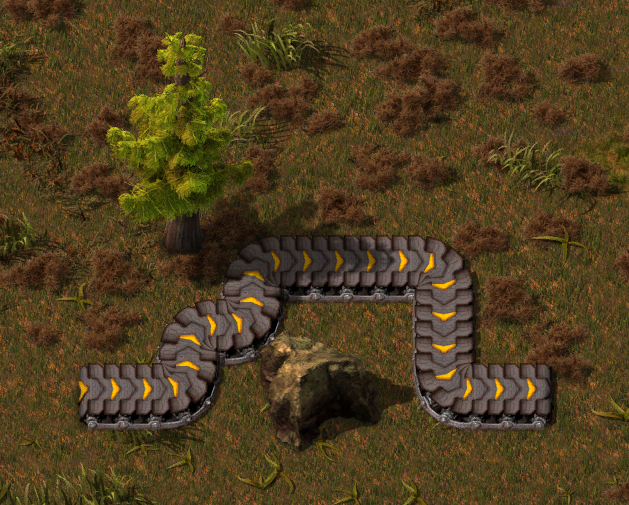
\includegraphics[width=0.8\textwidth]{img/factorio_complex-belt.png}
  \caption{Complex transport belt layout, avoiding a rock and a tree.}
  \label{fig:factorio_complex-belt}
\end{figure}

Finally, the compositions should also account for the machines taken up by the manufacturing.
Because in this domain we often use large numbers of machines, we use ``machine blocks'' to represent groups of machines performing the same recipe in parallel using common input and output flows.
These machine blocks integrate with logistics through these input and output flow locations.
Figure~\ref{fig:factorio_machine-block} depicts a block of four assembling machines in-game, all manufacturing iron gears from iron plates.

\begin{figure}[p]
  \centering
  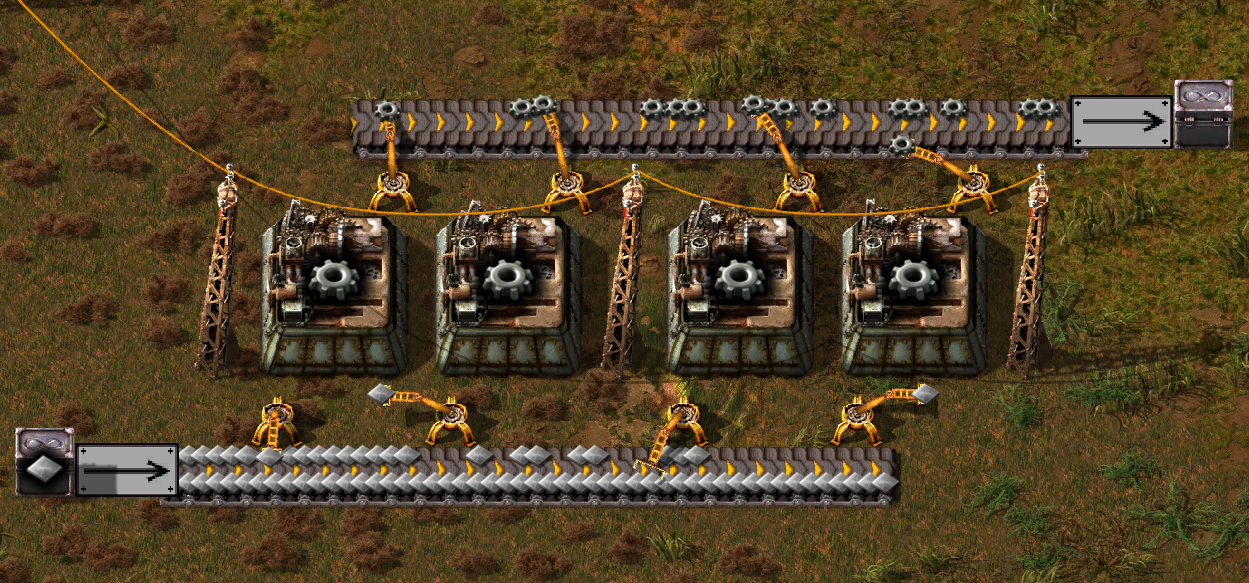
\includegraphics[width=\textwidth]{img/factorio_machine-block.png}
  \caption{Block of four assembling machines, all manufacturing iron gears from iron plates, with an input location on the left edge and output location on the right edge.}
  \label{fig:factorio_machine-block}
\end{figure}

We first define a domain with just item flows as resource atoms (see Section~\ref{sec:cases/factorio/item}) and primitive actions that represent logistics: splitting, merging and moving the flows (see Section~\ref{sec:cases/factorio/item-act}).
Then we extend this domain with machine blocks as further resource atoms (see Section~\ref{sec:cases/factorio/mach}), which allows us to represent manufacturing with a primitive action in the combined domain (see Section~\ref{sec:cases/factorio/manufacturing}).

As an application of the process models from this domain, we define how every valid composition can be turned into a sequence of instructions for its implementation in the game (see Section~\ref{sec:cases/factorio/instr}).
By mechanically following these instructions a player can implement the process.
Given a solution to the machine and logistics layout problems, an automated agent could also be made to mechanically follow these instructions.

This last part builds a text output (see Listing~\ref{lst:fourGears-instr} in Section~\ref{sec:cases/factorio/instr}) based on the given composition, so there is little we could gain by formalising it in Isabelle/HOL\@.
We instead implement it in Haskell on top of the formally verified code generated from the formalisation of this domain.

\subsection{Item Flows}
\label{sec:cases/factorio/item}

We start our formalisation of this domain by defining located flows of items.
For this we have to formalise locations, item types and rates of flow.

We only need locations to be uniquely identified, so that we know when two things are at the same location.
We choose to use string literals, rather than numeric identifiers, because they are more convenient when for example printed as part of the instructions.
The same reasoning applies when using string literals for action, item and machine labels in the rest of this section.
\begin{isadef}[Type synonym designating locations as string literals]{isa:factorio/loc}
  \isacomm{type-synonym}\ loc\ \isacharequal\ String.literal

\end{isadef}

We define item types simply by their label, such as an iron plate:
\begin{isadef}[Datatype for item types, with an example]{isa:factorio/item}
  \isacomm{datatype}\ item\ \isacharequal\ Item\ \isapars{\isafv{itemLabel}{\isacharcolon}\ String.literal}

\item
  \isacomm{definition}\ iron-plate\ \isacharequal\ Item\ \isaString{Iron\ Plate}

\end{isadef}

For rates of flow we use rational numbers (\isa{rat} in Isabelle/HOL).
They are sufficient to express rates and, compared to for instance the reals, their formalisation has a simple translation into executable code in the form of fractions.

Item flows simply combine the item type, rate of flow and location in one datatype:
\begin{isadef}[Datatype for flows of items]{isa:factorio/flow}
  \isacomm{datatype}\ flow\ \isacharequal\ Flow\ \isapars{\isafv{flowItem}{\isacharcolon}\ item}\ \isapars{\isafv{flowRate}{\isacharcolon}\ rat}\ \isapars{\isafv{flowLoc}{\isacharcolon}\ loc}

\end{isadef}

Because we will often be expressing item flows as individual resources, we define more convenient Isabelle notation for them:
\begin{isabelle}
\centering
  \isafv{item}\isalist{\isafv{rate}}\ \isanotation{at}\ \isafv{location}
\end{isabelle}
stands for:
\begin{isabelle}
\centering
  Res\ \isapars{Flow\ \isafv{item\ rate\ location}}
\end{isabelle}

\subsection{Logistics Actions}
\label{sec:cases/factorio/item-act}

We have five primitive actions representing logistics tools of the game for item flows (with first three shown in Figure~\ref{fig:factorio_move-split-merge}):
\begin{description}[style=nextline]
  \item[Moving a flow]
    Take a flow of given item type and rate from one location to another.
  \item[Splitting a flow]
    Split a flow into two flows of given rates.
    The rate the original flow must have is the sum of the given rates.
  \item[Merging flows]
    Take two flows of the same item at the same location and merge them into one.
  \item[Creating and empty flow]
    Create from nothing a flow of any item type at any location with zero rate.
  \item[Discarding an empty flow]
    Discard a flow of any item type at any location that has zero rate.
\end{description}

Before defining the actions themselves we specify the metadata they will carry.
In general, we use this data to support applications that inspect or consume compositions.
In this case, the application is the construction of a sequence of instructions for implementing the process.
Thus our metadata carries the information the user needs to implement each action.
We formalise the metadata in the same order as the inductive datatype \isa{flow{\isacharunderscore}meta} in Isabelle/HOL:
\begin{isadef}[Datatype for metadata of logistics actions]{isa:factorio/flow_meta}
  \isacomm{datatype}\ flow{\isacharunderscore}meta\ {\isacharequal}\isanewline
\ \ \isaindent{\isacharbar\ }Move\ \isapars{item}\ \isapars{rat}\ \isapars{loc}\ \isapars{loc}\isanewline
\ \ {\isacharbar}\ Split\ \isapars{item}\ \isapars{loc}\ \isapars{rat}\ \isapars{rat}\isanewline
\ \ {\isacharbar}\ Merge\ \isapars{item}\ \isapars{loc}\ \isapars{rat}\ \isapars{rat}\isanewline
\ \ {\isacharbar}\ Unit\ \isapars{item}\ \isapars{loc}\isanewline
\ \ {\isacharbar}\ Counit\ \isapars{item}\ \isapars{loc}

\end{isadef}

The processes in this domain then use item flows as linear atoms, no copyable atoms, string literals as labels and \isa{flow{\isacharunderscore}meta} as metadata.
We define the moving, merging and splitting of item flows as follows:
\begin{isadef}[Moving, splitting and merging flows of items]{isa:factorio/move_split_merge}
  \isacomm{definition}\ move\ {\isacharcolon}{\isacharcolon}\ {\isachardoublequoteopen}item\ {\isasymRightarrow}\ rat\ {\isasymRightarrow}\ loc\ {\isasymRightarrow}\ loc\isanewline
\isaindent{\isacomm{definition}\ move\ }{\isasymRightarrow}\ \isapars{flow,\ \isatv{c},\ String.literal,\ flow{\isacharunderscore}meta}\ process{\isachardoublequoteclose}\isanewline
\ \ \isaOcomm{where}\ {\isachardoublequoteopen}\isafv{move}\ \isabv{i\ r\ l\ k}\ {\isacharequal}\ Primitive\ {\isacharparenleft}\isabv{i}{\isacharbrackleft}\isabv{r}{\isacharbrackright}\ \isanotation{at}\ \isabv{l}{\isacharparenright}\ {\isacharparenleft}\isabv{i}{\isacharbrackleft}\isabv{r}{\isacharbrackright}\ \isanotation{at}\ \isabv{k}{\isacharparenright}\isanewline
\isaindent{\ \ \isaOcomm{where}{\isacharcolon}\ {\isachardoublequoteopen}\isafv{move}\ \isabv{i\ r\ l\ k}\ {\isacharequal}\ Primitive\ }\isaString{Move\ flow}\ {\isacharparenleft}Move\ \isabv{i\ r\ l\ k}{\isacharparenright}{\isachardoublequoteclose}%
\item
\isacomm{definition}\ split\ {\isacharcolon}{\isacharcolon}\ {\isachardoublequoteopen}item\ {\isasymRightarrow}\ loc\ {\isasymRightarrow}\ rat\ {\isasymRightarrow}\ rat\isanewline
\isaindent{\isacomm{definition}\ split\ }{\isasymRightarrow}\ \isapars{flow,\ \isatv{c},\ String.literal,\ flow{\isacharunderscore}meta}\ process{\isachardoublequoteclose}\isanewline
\ \ \isaOcomm{where}\ {\isachardoublequoteopen}\isafv{split}\ \isabv{i\ l\ r\ s}\ {\isacharequal}\ Primitive\ {\isacharparenleft}\isabv{i}{\isacharbrackleft}\isabv{r}{\isacharplus}\isabv{s}{\isacharbrackright}\ \isanotation{at}\ \isabv{l}{\isacharparenright}\ {\isacharparenleft}\isabv{i}{\isacharbrackleft}\isabv{r}{\isacharbrackright}\ \isanotation{at}\ \isabv{l}\ {\isasymodot}\ \isabv{i}{\isacharbrackleft}\isabv{s}{\isacharbrackright}\ \isanotation{at}\ \isabv{l}{\isacharparenright}\isanewline
\isaindent{\ \ \isaOcomm{where}\ {\isachardoublequoteopen}\isafv{split}\ \isabv{i\ l\ r\ s}\ {\isacharequal}\ Primitive\ }\isaString{Split\ flow}\ {\isacharparenleft}Split\ \isabv{i\ l\ r\ s}{\isacharparenright}{\isachardoublequoteclose}
\item
\isacomm{definition}\ merge\ {\isacharcolon}{\isacharcolon}\ {\isachardoublequoteopen}item\ {\isasymRightarrow}\ loc\ {\isasymRightarrow}\ rat\ {\isasymRightarrow}\ rat\isanewline
\isaindent{\isacomm{definition}\ merge\ }{\isasymRightarrow}\ \isapars{flow,\ \isatv{c},\ String.literal,\ flow{\isacharunderscore}meta}\ process{\isachardoublequoteclose}\isanewline
\ \ \isaOcomm{where}\ {\isachardoublequoteopen}\isafv{merge}\ \isabv{i\ l\ r\ s}\ {\isacharequal}\ Primitive\ {\isacharparenleft}\isabv{i}{\isacharbrackleft}\isabv{r}{\isacharbrackright}\ \isanotation{at}\ \isabv{l}\ {\isasymodot}\ \isabv{i}{\isacharbrackleft}\isabv{s}{\isacharbrackright}\ \isanotation{at}\ \isabv{l}{\isacharparenright}\ {\isacharparenleft}\isabv{i}{\isacharbrackleft}\isabv{r}{\isacharplus}\isabv{s}{\isacharbrackright}\ \isanotation{at}\ \isabv{l}{\isacharparenright}\isanewline
\isaindent{\ \ \isaOcomm{where}\ {\isachardoublequoteopen}\isafv{merge}\ \isabv{i\ l\ r\ s}\ {\isacharequal}\ Primitive\ }\isaString{Merge\ flows}\ {\isacharparenleft}Merge\ \isabv{i\ l\ r\ s}{\isacharparenright}{\isachardoublequoteclose}

\end{isadef}
\noindent
where, for instance, a \isa{merge\ \isafv{i\ l\ r\ s}} action takes two flows of the same item \isa{\isafv{i}} at the same location \isa{\isafv{l}} but with different rates \isa{\isafv{r}} and \isa{\isafv{s}}, and produces one with item and location unchanged but with summed rate.
The \isa{split} action does the opposite and the \isa{move} action changes only the location.
See Figure~\ref{fig:move-split-merge} for example diagrams of these actions and Figure~\ref{fig:factorio_move-split-merge} the in-game transport belt segments.

\begin{figure}[htbp]
  \centering
  \includesvg[scale=0.8]{img-gen/move-split-merge.svg}
  \caption{Process diagrams for example instances of \isa{move}, \isa{split} and \isa{merge}}
  \label{fig:move-split-merge}
\end{figure}

\begin{figure}[htbp]
  \centering
  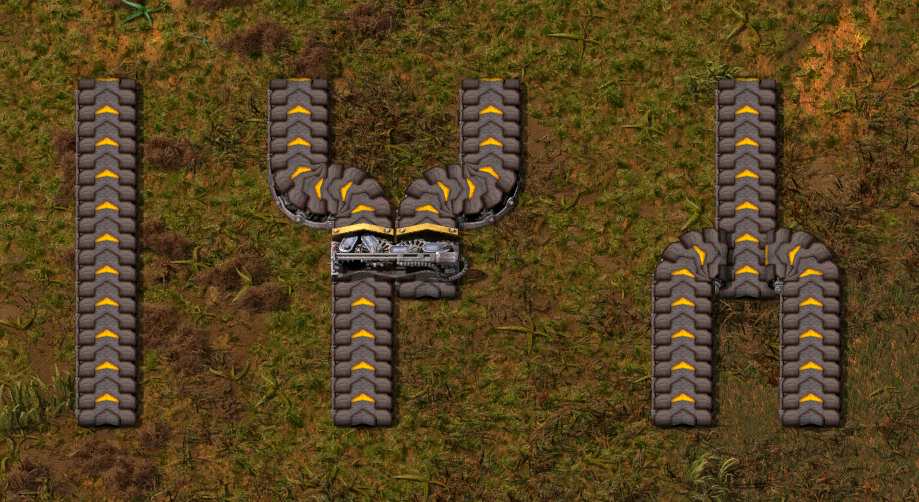
\includegraphics[width=\textwidth]{img/factorio_move-split-merge.png}
  \caption{Three transport belt segments representing the logistic actions \isa{move}, \isa{split} and \isa{merge} respectively.}
  \label{fig:factorio_move-split-merge}
\end{figure}

The remaining two actions represent our assumption that we can create and discard zero-rate flows for any item at any location.
We name these actions \isa{unit} and \isa{counit} and define them as follows, visualised with process diagrams in Figure~\ref{fig:unit-counit}:
\begin{isadef}[Creating and discarding zero-rate flows of items]{isa:factorio/unit_counit}
  \isacomm{definition}\isamarkupfalse%
\ unit\ {\isacharcolon}{\isacharcolon}\ {\isachardoublequoteopen}item\ {\isasymRightarrow}\ loc\ {\isasymRightarrow}\ \isapars{flow,\ \isatv{c},\ String.literal,\ flow{\isacharunderscore}meta}\ process{\isachardoublequoteclose}\isanewline
\ \ \isaOcomm{where}\ {\isachardoublequoteopen}\isafv{unit}\ \isabv{i\ l}\ {\isacharequal}\ Primitive\ Empty\ {\isacharparenleft}\isabv{i}{\isacharbrackleft}{\isadigit{0}}{\isacharbrackright}\ \isanotation{at}\ \isabv{l}{\isacharparenright}\ \isaString{Create\ zero\ flow}\ {\isacharparenleft}Unit\ \isabv{i\ l}{\isacharparenright}{\isachardoublequoteclose}
\item
\isacomm{definition}\isamarkupfalse%
\ counit\ {\isacharcolon}{\isacharcolon}\ {\isachardoublequoteopen}item\ {\isasymRightarrow}\ loc\ {\isasymRightarrow}\ \isapars{flow,\ \isatv{c},\ String.literal,\ flow{\isacharunderscore}meta}\ process{\isachardoublequoteclose}\isanewline
\ \ \isaOcomm{where}\ {\isachardoublequoteopen}\isafv{counit}\ \isabv{i\ l}\ {\isacharequal}\ Primitive\ {\isacharparenleft}\isabv{i}{\isacharbrackleft}{\isadigit{0}}{\isacharbrackright}\ \isanotation{at}\ \isabv{l}{\isacharparenright}\ Empty\ \isaString{Discard\ zero\ flow}\ {\isacharparenleft}Counit\ \isabv{i\ l}{\isacharparenright}{\isachardoublequoteclose}

\end{isadef}

\begin{figure}[htb]
  \centering
  \includesvg[scale=0.8]{img-gen/unit-counit.svg}
  \caption{Process diagrams for example instances of \isa{unit} and \isa{counit} actions}
  \label{fig:unit-counit}
\end{figure}

\subsection{Machine Blocks}
\label{sec:cases/factorio/mach}

Next we formalise machines and machine blocks, so that we can add them to the resource atoms and use them in manufacturing actions.
Machines are defined by their name, processing speed, base energy demand and running energy demand.
For instance, the electric furnace processes items at double of base speed, consumes $6\ kW$ of power while idle and an additional $180\ kW$ while running.
\begin{isadef}[Datatype for machines, with an example]{isa:factorio/machine}
  \isacomm{datatype}\ machine\ \isacharequal\isanewline
\ \ Machine\ \isapars{\isafv{machineLabel}{\isacharcolon}\ String.literal}\ \isapars{\isafv{machineSpeed}{\isacharcolon}\ rat}\isanewline
\isaindent{\ \ Machine\ }\isapars{\isafv{machineDrain}{\isacharcolon}\ nat}\ \isapars{\isafv{machineConsu}{\isacharcolon}\ nat}

\item
  \isacomm{definition}\ electric-furnace\ \isacharequal\ Machine\ \isaString{Electric\ Furnace}\ 2\ 6000\ 180000

\end{isadef}
\noindent
Note that the machine processing speed is a rational number to allow for machines taking more than base time (i.e.\ speed less than one).
The two energy demands, one when the machine is idle and one when it is running, are both natural numbers representing watts.

Machine blocks consist of the machine description, number of machines, input location and output location:
\pagebreak
\begin{isadef}[Datatype for blocks of machines working together]{isa:factorio/mach_block}
  \isacomm{datatype}\ mach-block\ \isacharequal\isanewline
\ \ MachBlock\ \isapars{\isafv{mblockMach}{\isacharcolon}\ machine}\ \isapars{\isafv{mblockCount}{\isacharcolon}\ nat}\isanewline
\isaindent{\ \ MachBlock\ }\isapars{\isafv{mblockIn}{\isacharcolon}\ loc}\ \isapars{\isafv{mblockOut}{\isacharcolon}\ loc}

\end{isadef}

As with item flows, we define more convenient Isabelle notation for machine blocks as individual resources:
\begin{isabelle}
\centering
  \isafv{mach}\isasymlangle\isafv{count}\isasymrangle\ \isanotation{at}\ \isafv{in-loc}\ \isanotation{\isasymrightarrow}\ \isafv{out-loc}
\end{isabelle}
stands for:
\begin{isabelle}
\centering
  Res\ \isapars{MachBlock\ \isafv{mach\ count\ in-loc\ out-loc}}
\end{isabelle}

\subsection{Manufacturing Action}
\label{sec:cases/factorio/manufacturing}

Manufacturing in our formalisation of this domain means using a block of machines to perform a recipe, converting one set of item flows into another.
Recipes are defined by two lists of item--count pairs (one for the inputs and one for the outputs), the base time required, the machine used and a name.
For instance, there is a recipe for crafting an iron gear from two iron plates, taking half a second and using a tier-one assembling machine.
\begin{isadef}[Datatype for manufacturing recipes, with an example]{isa:factorio/recipe}
  \isacomm{datatype}\isamarkupfalse%
\ recipe\ {\isacharequal}\isanewline
\ \ Recipe\ {\isachardoublequoteopen}\isapars{\isafv{recIn}{\isacharcolon}\ {\isacharparenleft}item\ {\isasymtimes}\ nat{\isacharparenright}\ list}{\isachardoublequoteclose}\ {\isachardoublequoteopen}\isapars{\isafv{recOut}{\isacharcolon}\ {\isacharparenleft}item\ {\isasymtimes}\ nat{\isacharparenright}\ list}{\isachardoublequoteclose}\isanewline
\isaindent{\ \ Recipe\ }\isapars{\isafv{recTime}{\isacharcolon}\ rat}\ \isapars{\isafv{recMach}{\isacharcolon}\ machine}\ \isapars{\isafv{recLab}{\isacharcolon}\ String{\isachardot}literal}

\item
  \isacomm{definition}\isamarkupfalse%
\ {\isachardoublequoteopen}craftGear\ {\isacharequal}\isanewline
\ \ Recipe\ {\isacharbrackleft}{\isacharparenleft}iron{\isacharunderscore}plate{\isacharcomma}\ {\isadigit{2}}{\isacharparenright}{\isacharbrackright}\ {\isacharbrackleft}{\isacharparenleft}iron{\isacharunderscore}gear{\isacharcomma}\ {\isadigit{1}}{\isacharparenright}{\isacharbrackright}\ {\isadigit{0}}{\isachardot}{\isadigit{5}}\ assembling{\isacharunderscore}machine{\isacharunderscore}{\isadigit{1}}\ \isaString{Craft\ Gear}

\end{isadef}

Performing a recipe with some number of machines in parallel requires flows of its inputs at one location and produces flows of its outputs at another location.
We define a function to help us construct these flows:
\begin{isadef}[Constructing a flow from recipe and machine information]{isa:factorio/stacksPerTimeAtSpeed}
  \isacomm{fun}\isamarkupfalse%
\ stacksPerTimeAtSpeed\ {\isacharcolon}{\isacharcolon}\ {\isachardoublequoteopen}rat\ {\isasymRightarrow}\ loc\ {\isasymRightarrow}\ nat\ {\isasymRightarrow}\ rat\ {\isasymRightarrow}\ item\ {\isasymtimes}\ nat\ {\isasymRightarrow}\ flow{\isachardoublequoteclose}\isanewline
\ \ \isaOcomm{where}\ {\isachardoublequoteopen}\isafv{stacksPerTimeAtSpeed}\ \isabv{t\ l\ n\ s}\ {\isacharparenleft}\isabv{i}{\isacharcomma}\isabv{c}{\isacharparenright}\ {\isacharequal}\ Flow\ \isabv{i}\ \isapars{\isabv{s}\ {\isacharasterisk}%
\ {\isacharparenleft}\isabv{n}{\isacharasterisk}\isabv{c}{\isacharparenright}\ {\isacharslash}\ \isabv{t}}\ \isabv{l}{\isachardoublequoteclose}

\end{isadef}
\noindent
which takes the recipe's time requirement \isa{\isabv{t}}, machine block location \isa{\isabv{l}}, number \isa{\isabv{n}} of parallel machines running the recipe, their processing speed \isa{\isabv{s}}, the item \isa{\isabv{i}} and its count \isa{\isabv{c}}, and constructs the corresponding item flow.
The last two arguments being taken as a pair is important to make this function suitable for mapping over the item--count lists with which recipes are defined.

The final piece of preparation is the metadata, which in this case collects the recipe, number of parallel instances, input location and output location:
\begin{isadef}[Datatype for metadata of the manufacturing action]{isa:factorio/manu_meta}
  \isacomm{datatype}\ manu{\isacharunderscore}meta\ {\isacharequal}\ Perform\ \isapars{recipe}\ \isapars{nat}\ \isapars{loc}\ \isapars{loc}

\end{isadef}

To express manufacturing actions, we move into a domain that combines both item flows and machine blocks.
This means that our processes now use as linear resource atoms the sum of those two types: \isa{flow\ \isacharplus\ mach{\isacharunderscore}block}.
Similarly, as metadata they use the sum of item flow and manufacturing metadata: \isa{flow{\isacharunderscore}meta\ \isacharplus\ manu{\isacharunderscore}meta}.
The two constructors of Isabelle's sum type, which inject a value from either summand into the sum type, are \isa{Inl\ \ty\ \isatv{a}\ \isasymRightarrow\ \isatv{a}\ \isacharplus\ \isatv{b}} and \isa{Inr\ \ty\ \isatv{b}\ \isasymRightarrow\ \isatv{a}\ \isacharplus\ \isatv{b}}.

We use a recipe, number of machines to use and two locations to define the manufacturing primitive action \isa{perform} as follows:
\begin{isadef}[Performing a recipe with a block of machines]{isa:factorio/perform}
  \isacomm{fun}\ perform\ {\isacharcolon}{\isacharcolon}\ {\isachardoublequoteopen}recipe\ {\isasymRightarrow}\ nat\ {\isasymRightarrow}\ loc\ {\isasymRightarrow}\ loc\isanewline
\isaindent{\isacomm{fun}\ perform\ {\isacharcolon}{\isacharcolon}\ }{\isasymRightarrow}\ {\isacharparenleft}flow\ {\isacharplus}\ mach{\isacharunderscore}block{\isacharcomma}\ \isatv{c},\isanewline
\isaindent{\isacomm{fun}\ perform\ {\isacharcolon}{\isacharcolon}\ {\isasymRightarrow}\ {\isacharparenleft}fl}String{\isachardot}literal{\isacharcomma}\ flow{\isacharunderscore}meta\ {\isacharplus}\ manu{\isacharunderscore}meta{\isacharparenright}\ process{\isachardoublequoteclose}\isanewline
\ \ \isaOcomm{where}\ {\isachardoublequoteopen}\isafv{perform}\ {\isacharparenleft}Recipe\ \isabv{ins\ outs\ time\ m\ name}{\isacharparenright}\ \isabv{n\ l1\ l2}\ {\isacharequal}\isanewline
\ \ Primitive\isanewline
\ \ \ \ {\isacharparenleft}\ Parallel\ {\isacharparenleft}map\ {\isacharparenleft}Res\ {\isasymcirc}\ Inl\ {\isasymcirc}\ stacksPerTimeAtSpeed\ \isabv{time}\ \isabv{l1}\ \isabv{n}\ {\isacharparenleft}machineSpeed\ \isabv{m}{\isacharparenright}{\isacharparenright}\isanewline
\isaindent{\ \ \ \ {\isacharparenleft}\ Parallel\ {\isacharparenleft}map\ }\isabv{ins}{\isacharparenright}\ {\isasymodot}\isanewline
\ \ \ \ \isaindent{\isacharparenleft}\ Res\ {\isacharparenleft}Inr\ {\isacharparenleft}MachBlock\ \isabv{m\ n\ l1\ l2}{\isacharparenright}{\isacharparenright}{\isacharparenright}\isanewline
\ \ \ \ {\isacharparenleft}\ Parallel\ {\isacharparenleft}map\ {\isacharparenleft}Res\ {\isasymcirc}\ Inl\ {\isasymcirc}\ stacksPerTimeAtSpeed\ \isabv{time\ l2\ n}\ {\isacharparenleft}machineSpeed\ \isabv{m}{\isacharparenright}{\isacharparenright}\isanewline
\isaindent{\ \ \ \ {\isacharparenleft}\ Parallel\ {\isacharparenleft}map\ }\isabv{outs}{\isacharparenright}{\isacharparenright}\isanewline
\ \ \ \ \isabv{name}\isanewline
\ \ \ \ {\isacharparenleft}\ Inr\ {\isacharparenleft}Perform\ {\isacharparenleft}Recipe\ \isabv{ins\ outs\ time\ m\ name}{\isacharparenright}\ \isabv{n\ l1\ l2}{\isacharparenright}{\isacharparenright}{\isachardoublequoteclose}

\end{isadef}
\noindent
where the input resource is a parallel combination of item flows (one for each input item of the recipe) along with a suitable block of machines.
The output resource is a parallel combination of only the item flows for the recipe's outputs.
The function \isa{machineSpeed} merely projects the second argument from the \isa{Machine} constructor, its processing speed.

Figure~\ref{fig:perform} shows an example diagram of the \isa{perform} action, using a recipe for making train cargo wagons.
It takes as input three item flows of the recipe ingredients (iron gears, iron plates, steel plates) arriving at the location named ``Source'' and the two assembling machines used to perform the recipe.
Those machines take inputs from ``Source'' and deposit their products at another location named ``Destination''.
See Figure~\ref{fig:fourGears} for further instances of this action.

\begin{figure}[htbp]
  \centering
  \includesvg[width=\textwidth]{img-gen/perform.svg}
  \caption{Process diagram for crafting cargo wagons on two machines in parallel.}
  \label{fig:perform}
\end{figure}

The machine block is consumed by this action to represent occupying those machines with continuous production.
This prevents us from using the same group of machines for two tasks at the same time.
The block's locations are set to match those where the input and output flows are generated, and its size is set to match the multiplier used to compute the flow rates.

With all the primitive actions set up we can proceed with constructing compositions.
In the following two sections we describe one such composition and how instructions are mechanically generated from such compositions.

From this point on we work in the combined domain, so we redefine our custom notation to use the appropriate injections.
The item flow notation \isa{\isafv{item}\isalist{\isafv{rate}}\ \isanotation{at}\ \isafv{location}} and the machine block notation \isa{\isafv{mach}\isasymlangle\isafv{count}\isasymrangle\ \isanotation{at}\ \isafv{in-loc}\ \isanotation{\isasymrightarrow}\ \isafv{out-loc}} now apply \isa{Inl} and \isa{Inr} respectively before constructing the resource atom.

Note that all processes from the item flow domain can be easily translated into the combined domain.
We just apply the left injection constructor \isa{Inl} to all linear resource atoms and metadata (leaving copyable atoms and labels unchanged) through the process map: \isa{map{\isacharunderscore}process\ Inl\ id\ id\ Inl}.
This map is defined automatically by Isabelle thanks to the BNF structure of resources (see Section~\ref{sec:res/bnf}).
See Section~\ref{sec:proc/transform} for a discussion of such systematic transformations of processes.

\subsection{Example Composition: Four Iron Gears}
\label{sec:cases/factorio/gears}

As an example composition we consider the process of turning iron ore into four iron gears per second.
This has two manufacturing steps: the iron ore must be smelted into plates and those then crafted into gears.
More precisely, considering the flow rates and locations, the process has four steps:
\begin{enumerate}
  \item Smelt iron ore into plates with $13$ furnaces in parallel.
  \item Split the resulting iron plates into two flows with rates $0.125$ and $8$.
  \item Move $8$ iron plates per second to the next location.
  \item Craft iron plates into gears with $4$ assembly machines in parallel.
\end{enumerate}

Our choice of targeting 100\% machine utilisation means that the furnaces produce more iron plates than we need, which could be made available to another process later on.
Alternatively, one could relax the utilisation requirement to require for $n$ machines utilisation of at least $\frac{n - 1}{n}$, meaning at most one machine from the group is not fully utilised.
Then the action of performing a recipe could be given a fractional number of parallel instances to meet any rational output flow rate.
We go with the 100\% requirement that sometimes yields a surplus, but our composition rules ensure that it is correctly accounted for and never lost (see Section~\ref{sec:proc/valid}).

The earlier four steps are reflected in the actual process composition, which is shown in Figure~\ref{fig:fourGears}:
Note that this composition is parameterised by the four involved locations, as they only have to be kept consistent between the individual actions.
In the second and third steps we translate logistics action, splitting and moving a flow respectively, into the combined domain using the process mapper.

\begin{figure}[htbp]
  \begin{subfigure}{\textwidth}
    \begin{isabelle}
      \isacomm{definition}\isamarkupfalse%
\ {\isachardoublequoteopen}\isafv{fourGears}\ \isabv{lIPlateIn\ lIPlateOut\ lGearIn\ lGearOut}\ {\isacharequal}\isanewline
\ \ \ \ {\isacharparenleft}\ perform\ smeltIronOre\ {\isadigit{1}}{\isadigit{3}}\ \isabv{lIPlateIn}\ \isabv{lIPlateOut}\ {\isasymparallel}\isanewline
\ \ \ \ \ \ Identity\ {\isacharparenleft}assembling{\isacharunderscore}machine{\isacharunderscore}{\isadigit{1}}{\isacharless}{\isadigit{4}}{\isachargreater}\isanotation{\ at\ }\isabv{lGearIn}\ {\isanotation{\isasymrightarrow}}\ \isabv{lGearOut}{\isacharparenright}{\isacharparenright}\ {\isacharsemicolon}{\isacharsemicolon}\isanewline
\ \ \ \ {\isacharparenleft}\ map{\isacharunderscore}process\ Inl\ id\ id\ Inl\ \isapars{split\ iron{\isacharunderscore}plate\ \isabv{lIPlateOut}\ {\isadigit{0}}{\isachardot}{\isadigit{1}}{\isadigit{2}}{\isadigit{5}}\ {\isadigit{8}}}\ {\isasymparallel}\isanewline
\ \ \ \ \ \ Identity\ {\isacharparenleft}assembling{\isacharunderscore}machine{\isacharunderscore}{\isadigit{1}}{\isacharless}{\isadigit{4}}{\isachargreater}\isanotation{\ at\ }\isabv{lGearIn}\ {\isanotation{\isasymrightarrow}}\ \isabv{lGearOut}{\isacharparenright}{\isacharparenright}\ {\isacharsemicolon}{\isacharsemicolon}\isanewline
\ \ \ \ {\isacharparenleft}\ Identity\ {\isacharparenleft}iron{\isacharunderscore}plate{\isacharbrackleft}{\isadigit{0}}{\isachardot}{\isadigit{1}}{\isadigit{2}}{\isadigit{5}}{\isacharbrackright}\isanotation{\ at\ }\isabv{lIPlateOut}{\isacharparenright}\ {\isasymparallel}\isanewline
\ \ \ \ \ \ map{\isacharunderscore}process\ Inl\ id\ id\ Inl\ \isapars{move\ iron{\isacharunderscore}plate\ {\isadigit{8}}\ \isabv{lIPlateOut}\ \isabv{lGearIn}}\ {\isasymparallel}\isanewline
\ \ \ \ \ \ Identity\ {\isacharparenleft}assembling{\isacharunderscore}machine{\isacharunderscore}{\isadigit{1}}{\isacharless}{\isadigit{4}}{\isachargreater}\isanotation{\ at\ }\isabv{lGearIn}\ {\isanotation{\isasymrightarrow}}\ \isabv{lGearOut}{\isacharparenright}{\isacharparenright}\ {\isacharsemicolon}{\isacharsemicolon}\isanewline
\ \ \ \ {\isacharparenleft}\ Identity\ {\isacharparenleft}iron{\isacharunderscore}plate{\isacharbrackleft}{\isadigit{0}}{\isachardot}{\isadigit{1}}{\isadigit{2}}{\isadigit{5}}{\isacharbrackright}\isanotation{\ at\ }\isabv{lIPlateOut}{\isacharparenright}\ {\isasymparallel}\isanewline
\ \ \ \ \ \ perform\ craftGear\ {\isadigit{4}}\ \isabv{lGearIn}\ \isabv{lGearOut}{\isacharparenright}{\isachardoublequoteclose}

    \end{isabelle}
    \caption{Definition of the process. We use \isa{\isacharsemicolon\isacharsemicolon} and \isa{\isasymparallel} as infix notation in Isabelle for sequential and parallel composition respectively.}
  \end{subfigure}
  \\~\\
  \begin{subfigure}{\textwidth}
    \centering
    \includesvg[width=\textwidth]{img/fourGears-cutup.svg}
    \caption{Process diagram.}
  \end{subfigure}
  \caption{Process definition and diagram for crafting iron gears from ore}
    \label{fig:fourGears}
\end{figure}

On top of the four core steps, the above composition also involves identity processes that ensure resources that are not being used in a given step are carried safely to the next.
One can find a pattern to these accommodations and define helper functions to more easily insert the identity processes, but we omit this to keep the example more direct.

Now we briefly discuss what implications there are from the validity of this composition, and more generally other compositions in this domain.
As discussed in Section~\ref{sec:proc/valid}, process composition validity in general requires that resources match on both sides of a connection.

Because two item flows are only equal if their rates are equal, we know that there is no bottleneck introduced from the connections made by the composition.
Then, because all of the manufacturing actions are set to run their machines at full capacity, we know the whole process will be running at 100\% utilisation.

Furthermore, item flows are also only equal if their locations are equal, which means that any change in item locations must come from primitive actions --- in our case either a movement or a manufacturing action.
Therefore these primitive actions describe all the required logistics connections.

Finally, the input and output of the composition tell us:
\begin{itemize}
  \item What items the process needs to keep working;
  \item What items it will produce;
  \item What kind of production capacity (i.e.\ machines) it requires to do so.
\end{itemize}
This information, along with the primitive actions contained in the composition, is all we need to generate instructions for implementing the composition as a factory in the game.
We discuss these instructions next, focusing on the process composition we introduced above.

\subsection{Generating User Instructions}
\label{sec:cases/factorio/instr}

We generate a sequence of instructions that can be mechanically carried out to build the factory.
In these we instruct the user on the placement and connection of the various machines.

Implementing our process compositions as factories in the game requires laying out each individual machine in the world and precisely routing the logistics connections.
In the absence of a fully automated solution for this problem, we rely on a human player to carry out the instructions.
The instructions may state that two locations should be connected, but they do not try to specify how exactly that connection should look in terms of coordinates.
However, if this layout is automated in the future, then our instructions could be adapted for an automated agent.

The instructions (see Listing~\ref{lst:fourGears-instr} for an example) are split into four parts:
\begin{itemize}
  \item Requirements, which are generated from the process input and state what item flows and machines need to be provided.
  \item Actions, which are generated from the primitive actions in the composition and describe how those should be implemented.
    For manufacturing this means describing the recipe and the machine block to use.
    For movement this means describing the item type, minimum required throughput, origin and destination.
  \item Effects, which are generated from the process output and state what item flows (and potentially unused machines) we get out of the process.
  \item Energy demand, which is calculated from the energy drain of machines consumed by the process.
    The fact that all used machines are fully utilised makes this calculation a simple sum.
\end{itemize}

\begin{lstlisting}[label=lst:fourGears-instr,caption=Instructions for the \isa{fourGears} composition,basicstyle=\small\ttfamily,columns=flexible,breaklines=true]
Process composition "fourGears":
Requirements:
 - Have Iron Ore arriving to iron-smelter-in at the rate of 65/8 per second
 - Have 13 of Electric Furnace taking inputs from iron-smelter-in and passing outputs to iron-smelter-out
 - Have 4 of Assembling Machine 1 taking inputs from gears-in and passing outputs to gears-out
Actions:
 - Set 13 of Electric Furnace to perform recipe "Smelt Iron Ore to Iron Plate" on inputs from iron-smelter-in and pushing outputs to iron-smelter-out
 - Split flow of Iron Plate located at iron-smelter-out from rate 65/8 per second into 1/8 per second and 8 per second
 - Move 8 per second of Iron Plate from iron-smelter-out to gears-in
 - Set 4 of Assembling Machine 1 to perform recipe "Craft Iron Plates into Iron Gear" on inputs from gears-in and pushing outputs to gears-out
Effects:
 - Have Iron Plate arriving to iron-smelter-out at the rate of 1/8 per second
 - Have Iron Gear arriving to gears-out at the rate of 4 per second
Energy demand: 2728000 W
\end{lstlisting}

The way we generate these instructions is the only part of our work on this domain that is outside of the proof assistant.
We use Haskell code automatically generated by Isabelle/HOL for all of the above definitions, including the \isa{fourGears} composition.
On top of this code we implement a number of functions for pretty-printing the data involved, such as printing the fully formal natural numbers as plain integers, and construct the actual instructions.
We construct individual instructions by taking the relevant part of the composition (e.g.\ its input or primitive actions) and expressing it in natural language.

We validated the above instructions for the \isa{fourGears} composition by carrying them out in-game, with the result shown in Figure~\ref{fig:factorio_four-gears}.
The resulting factory exhibits no bottlenecks between the machine blocks, just as validity of the composition predicts.
Furthermore, the production rates recorded by the simulation engine match those in the composition, and the recorded energy demand matches the one calculated from the consumed machines.
The only difficulty we encountered in following the instructions is implementing the precise item flow split ratio (in this case $1:64$) with the simple logistics tools made available (a $1:1$ splitter).

\begin{figure}[htbp]
  \centering
  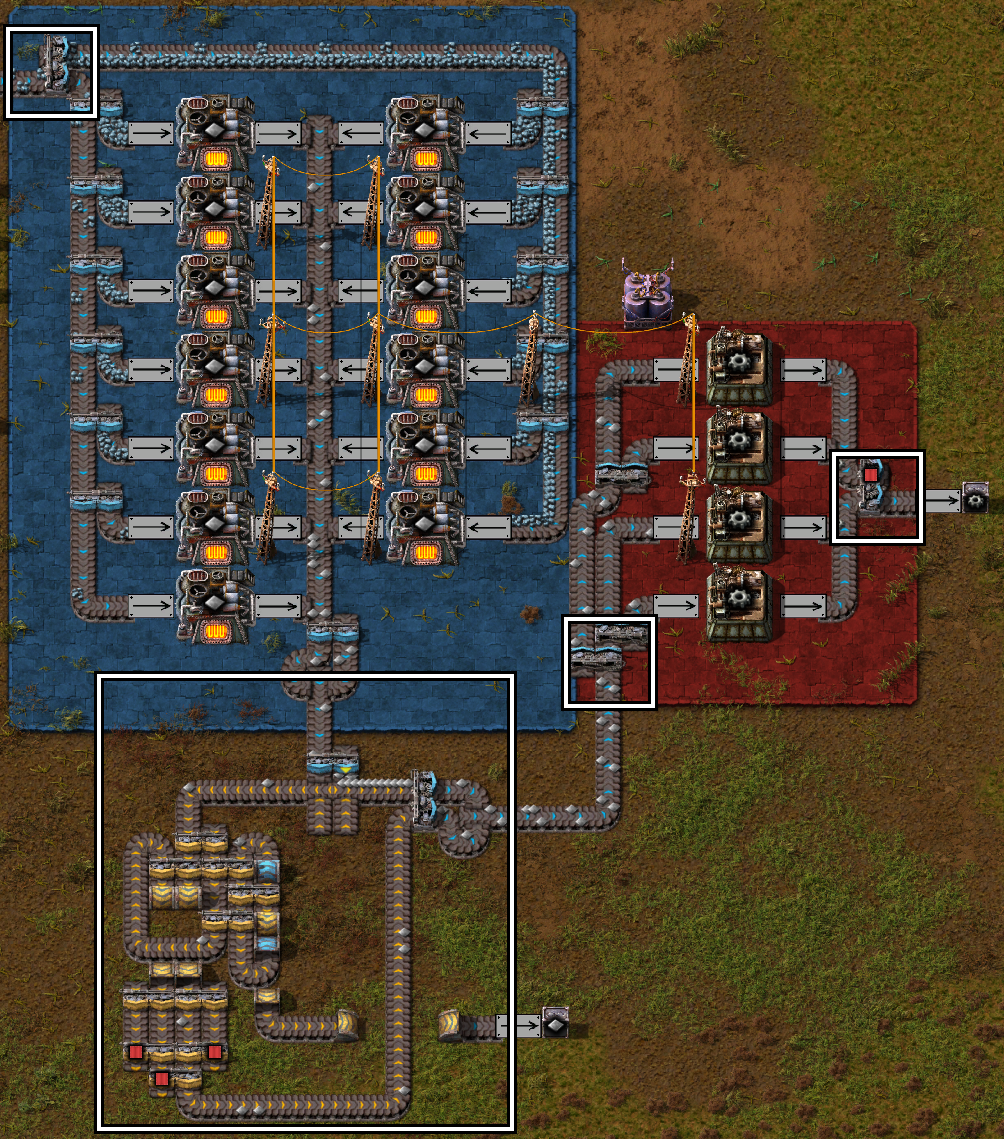
\includegraphics[width=\textwidth]{img/factorio_four-gears.png}
  \caption{In-game implementation of the \isa{fourGears} composition with the electric furnace block highlighted in blue and assembling machine block highlighted in red. The four named locations are highlighted with black-white squares. Bottom segment achieves the $1:64$ split of iron plates.}
  \label{fig:factorio_four-gears}
\end{figure}

\subsection{Possible Extensions}
\label{sec:cases/factorio/extensions}

While our formalisation of this domain is already non-trivial, there are still many aspects of Factorio that we do not model.
However, most of those could be modelled with our framework.
We note some here as possible future work extending this case study.

For instance, we currently only formalise solid manufacturing, while Factorio also involves fluids.
These have their own logistics system through the use of pipes, pumps and tanks.
They could be included in a way analogous to the item flows, while extending recipes and manufacturing actions to include them.

Another aspect we do not currently model in its entirety is fuel consumption.
We constrain ourselves only to machines that consume electricity, while the game also includes ones that consume solid or fluid fuels.
This could be included as a further input to performing a recipe, using the time taken, energy drain and energy value of a given fuel to compute how much is needed.

Beyond aspects of the game that we do not model, we could also improve the integration of our formalisation with the game.
At present, we manually encode the item types, machines and recipes that we use.
However, Factorio allows us to export the whole range of item types, machines and recipes from a running copy of the game as a JSON file.
We could load this data into Isabelle to make it all available to our formalisation with values guaranteed to be accurate.

\section{Conclusion}
\label{sec:cases/conc}

In this chapter we gave a number of case studies to demonstrate the main features of our framework.
We touch on a variety of domains: education, daily life and manufacturing.
The case studies we presented suggest some of the possible uses of our framework and the tools that could be based on it.

In the next chapter we conclude the thesis, tying together the thread running through it and giving a brief overview of potential future work.

\ifstandalone
\bibliographystyle{plainurl}
\bibliography{references}
\fi

\end{document}

\documentclass[class=smolathesis,crop=false]{standalone}

\begin{document}

\chapter{Conclusion}
\label{ch:conc}

In the preceding chapters we developed a framework for verified composition of processes based on linear resources.
We did so in the proof assistant Isabelle/HOL to ensure a high degree of confidence in the framework's properties and to allow for automated generation of executable code.

We connected our process compositions to two other concepts: linear logic deductions and port graphs.
The first focuses on the correspondence of deduction in linear logic to the structure of correct processes, while the second focuses on viewing large processes as collections of actions connected by their inputs and outputs.
We use both to demonstrate that valid process compositions manipulate resources correctly.

We also explored an extension of our framework to include probabilistic information in its description of non-determinism.
While the present outcome of this exploration is open to definite improvements, it did demonstrate how invaluable a proof assistant is in exploring changes to the foundations of a formal framework.
With its assistance, making such changes is significantly easier and, as a result, exploratory studies of formalised systems become more viable.

We demonstrated the application of our framework with a number of case studies in different domains.
While these do not cover the full breadth of possibility, they illustrate the framework's main features and suggest more complex uses.

\section{Future Work}
\label{sec:conc/future}

In this section we highlight some of the main threads of future work arising from this thesis.

\paragraph*{Process behaviour.}
A formalisation of behaviour for our process compositions would allow us to prove which of the latter, although syntactically distinct, represent the same behaviour.
This in turn would allow us to verify, for instance, behaviour-preserving simplifications of process compositions such as removing identity actions from sequential composition.

We see process port graphs from Section~\ref{sec:port_graphs/process} and the transition system for port graphs from Section~\ref{sec:port_graphs/trans} as providing a promising path towards formalising a notion of behaviour for our process compositions.
A future task for this thread lies in expanding our formalisation of port graphs so that they can capture non-determinism and higher-order processes.

\paragraph*{Connection to other formalisms.}
A complementary approach to process composition behaviour would be to formally connect them to other process formalisms, such as $\pi$-calculus or Petri nets.
We could then use their established theory and tools in our framework.
That includes making use of the their transition systems to characterise the behaviour of our process compositions.

In order to mechanise the connection, we would require mechanisations of those process formalisms in Isabelle/HOL.
There exists such a mechanisation for the $\pi$-calculus due to Bengtson~\cite{Pi_Calculus-AFP}.
As far as we are aware, there is no published mechanisation of Petri nets in Isabelle/HOL.

Both of these formalisms make use of connections between individual actions: as channels between agents in $\pi$-calculus and as places between transitions in Petri nets.
As such, we believe a significant part of formally connecting process compositions to them would be handled by process port graphs.
Then, beyond finding a suitable mechanisation of the target formalism, the major task would be connecting to it from port graphs.

\paragraph*{Probabilistic information.}
As noted, the outcome of our exploration of probabilistic resources in Chapter~\ref{ch:prob} is relatively preliminary.
While the extended framework can express the probabilistic information and make use of it in computing expected values from process compositions, it produces impractically complex resource expressions.
As such, one thread of future work would be about revising how probabilistic information can be better integrated into resources and process compositions in light of lessons learned through our exploration.

\paragraph*{Concrete tools.}
Mechanising our framework in Isabelle/HOL allows us to automatically generate executable code from it.
We make use of it to generate process diagrams (see Section~\ref{sec:proc/diag}) and in our model of manufacturing in Factorio to generate instructions for implementing a process as a factory (see Section~\ref{sec:cases/factorio/instr}).

There are more tools we could implement by utilising the verified code generated by Isabelle/HOL, boosting the practicality of our framework.
For instance, recall our definition of process port graphs (see Section~\ref{sec:port_graphs/process}) and our conversion of port graphs into a format that can be visualised by the Eclipse Layout Kernel and Sprotty (see Section~\ref{sec:port_graphs/mech/export}).
We could make use of the verified code for these to implement a visualisation tool tailored to process compositions.
Unlike our process diagrams, such a tool could be made interactive, allowing us to better inspect the process in question or even construct processes in a graphical environment.

We could additionally make use of the port graph transition system (see Section~\ref{sec:port_graphs/trans}) to identify enabled actions.
Then we could distinguish the relevant nodes in the visualisation, forming a kind of graphical checklist for the process.
It could be made interactive, allowing users to mark actions as completed to update the highlighted set of enabled actions.
We believe this would aid coordination in settings where multiple people cooperate to execute a large process.

Our ability to generate verified code in Scala, Haskell, OCaml and SML offers the opportunity to integrate with a wide variety of external frameworks while retaining the rigour of our formally verified approach.

\section{Concluding Remarks}
\label{sec:conc/remarks}

Our mechanised framework gives us a solid foundation for tools whose implementation of processes can be checked, so that the assistance they provide can be relied upon.
The language of process compositions is simple and avoids ambiguity, so that our expectations are clear both when modelling processes and when using those models.
Moreover, the verified code generated by Isabelle ensures that what the tools use is what we formalised.

Looking toward the future, we will use this foundation to build such tools and expand the range of domains where we have applied our framework.
Reaching more domains and modelling increasingly complex processes will allow us to truly push the framework to its limits, and then, with the assistance of Isabelle, expand those limits in a rigorous way.

With the formalisations presented in this thesis, we can implement, for instance, a graphical checklist to help large teams coordinate their work on complex processes in potentially safety-critical situations.
The formal basis, given an accurate specification, will ensure that no team member is left without what they need or not knowing what they have to do, and that the graphical representation is faithful to the underlying process model.
We believe this would help support people in a variety of domains, from manufacturing through administration all the way to healthcare.

It is our aim to leverage the best abilities of machines to help people perform complex tasks.
We have helped machines understand how processes are structured, and now we can make them better at assisting us.

\ifstandalone
\bibliographystyle{plainurl}
\bibliography{references}
\fi

\end{document}


\appendix

\documentclass[class=smolathesis,crop=false]{standalone}

\begin{document}

\chapter{Appendix}
\label{ch:appendix}

\section{ILL Deduction Embedding Functions}
\label{app:ill-deduct}

The conclusions of deeply embedded ILL deductions (see Section~\ref{sec:linearity/deep}) are represented by values from the \isa{ill-sequent} datatype, capturing the antecedents and consequent:
\begin{isadef}[Datatype for arbitrary ILL sequents]{isa:ill_sequent}
  \isacomm{datatype}\isamarkupfalse%
\ \isatv{a}\ ill{\isacharunderscore}sequent\ {\isacharequal}\ Sequent \isapars{{\isachardoublequoteopen}\isatv{a}\ ill{\isacharunderscore}prop\ list{\isachardoublequoteclose}} \isapars{{\isachardoublequoteopen}\isatv{a}\ ill{\isacharunderscore}prop{\isachardoublequoteclose}}

\end{isadef}

We tie those values to the shallowly embedded relation of valid sequents (see Section~\ref{sec:linearity/shallow}) through the \isa{ill-sequent-valid} function:
\begin{isadef}[Validity predicate on ILL sequents]{isa:ill_sequent_valid}
  \isacomm{primrec}\isamarkupfalse%
\ ill{\isacharunderscore}sequent{\isacharunderscore}valid\ {\isacharcolon}{\isacharcolon}\ {\isachardoublequoteopen}\isatv{a}\ ill{\isacharunderscore}sequent\ {\isasymRightarrow}\ bool{\isachardoublequoteclose}\isanewline
\ \ \isaOcomm{where}\ {\isachardoublequoteopen}\isafv{ill{\isacharunderscore}sequent{\isacharunderscore}valid}\ {\isacharparenleft}Sequent\ \isabv{a\ c}{\isacharparenright}\ {\isacharequal}\ \isabv{a}\ {\isasymturnstile}\ \isabv{c}{\isachardoublequoteclose}

\end{isadef}

We set up a declaration bundle \isa{deep-sequent} which we can use to switch the turnstile notation from the relation to these values:
\begin{isadef}[Declaration bundle switching turnstile notation]{isa:deep_sequent}
  \isacomm{bundle}\isamarkupfalse%
\ deep{\isacharunderscore}sequent\ %
\isaOcomm{begin}\isanewline
\isanewline
\isacomm{no{\isacharunderscore}notation}\isamarkupfalse%
\ sequent\ {\isacharparenleft}\isaOcomm{infix}\ {\isachardoublequoteopen}{\isasymturnstile}{\isachardoublequoteclose}\ {\isadigit{6}}{\isadigit{0}}{\isacharparenright}\isanewline
\isacomm{notation}\isamarkupfalse%
\ Sequent\ {\isacharparenleft}\isaOcomm{infix}\ {\isachardoublequoteopen}{\isasymturnstile}{\isachardoublequoteclose}\ {\isadigit{6}}{\isadigit{0}}{\isacharparenright}\isanewline
\isanewline
\isaOcomm{end}\isamarkupfalse%

\end{isadef}

The full definition for conclusions of deeply embedded ILL deductions is then as follows:
\begin{isadef}[Conclusions of deeply embedded ILL deductions]{isa:ill_conclusion}
  \isacomm{primrec}\ ill{\isacharunderscore}conclusion\ {\isacharcolon}{\isacharcolon}\ {\isachardoublequoteopen}{\isacharparenleft}\isatv{a}{\isacharcomma}\ \isatv{l}{\isacharparenright}\ ill{\isacharunderscore}deduct\ {\isasymRightarrow}\ \isatv{a}\ ill{\isacharunderscore}sequent{\isachardoublequoteclose}\ \isaOcomm{where}\isanewline
\ \ \ \ {\isachardoublequoteopen}\isafv{ill{\isacharunderscore}conclusion}\ {\isacharparenleft}Premise\ \isabv{G}\ \isabv{c}\ \isabv{l}{\isacharparenright}\ {\isacharequal}\ \isabv{G}\ {\isasymturnstile}\ \isabv{c}{\isachardoublequoteclose}\isanewline
\ \ {\isacharbar}\ {\isachardoublequoteopen}\isafv{ill{\isacharunderscore}conclusion}\ {\isacharparenleft}Identity\ \isabv{a}{\isacharparenright}\ {\isacharequal}\ {\isacharbrackleft}\isabv{a}{\isacharbrackright}\ {\isasymturnstile}\ \isabv{a}{\isachardoublequoteclose}\isanewline
\ \ {\isacharbar}\ {\isachardoublequoteopen}\isafv{ill{\isacharunderscore}conclusion}\ {\isacharparenleft}Exchange\ \isabv{G}\ \isabv{a}\ \isabv{b}\ \isabv{D}\ \isabv{c}\ \isabv{P}{\isacharparenright}\ {\isacharequal}\ \isabv{G}\ {\isacharat}\ {\isacharbrackleft}\isabv{b}{\isacharbrackright}\ {\isacharat}\ {\isacharbrackleft}\isabv{a}{\isacharbrackright}\ {\isacharat}\ \isabv{D}\ {\isasymturnstile}\ \isabv{c}{\isachardoublequoteclose}\isanewline
\ \ {\isacharbar}\ {\isachardoublequoteopen}\isafv{ill{\isacharunderscore}conclusion}\ {\isacharparenleft}Cut\ \isabv{G}\ \isabv{b}\ \isabv{D}\ \isabv{E}\ \isabv{c}\ \isabv{P}\ \isabv{Q}{\isacharparenright}\ {\isacharequal}\ \isabv{D}\ {\isacharat}\ \isabv{G}\ {\isacharat}\ \isabv{E}\ {\isasymturnstile}\ \isabv{c}{\isachardoublequoteclose}\isanewline
\ \ {\isacharbar}\ {\isachardoublequoteopen}\isafv{ill{\isacharunderscore}conclusion}\ {\isacharparenleft}TimesL\ \isabv{G}\ \isabv{a}\ \isabv{b}\ \isabv{D}\ \isabv{c}\ \isabv{P}{\isacharparenright}\ {\isacharequal}\ \isabv{G}\ {\isacharat}\ {\isacharbrackleft}\isabv{a}\ {\isasymotimes}\ \isabv{b}{\isacharbrackright}\ {\isacharat}\ \isabv{D}\ {\isasymturnstile}\ \isabv{c}{\isachardoublequoteclose}\isanewline
\ \ {\isacharbar}\ {\isachardoublequoteopen}\isafv{ill{\isacharunderscore}conclusion}\ {\isacharparenleft}TimesR\ \isabv{G}\ \isabv{a}\ \isabv{D}\ \isabv{b}\ \isabv{P}\ \isabv{Q}{\isacharparenright}\ {\isacharequal}\ \isabv{G}\ {\isacharat}\ \isabv{D}\ {\isasymturnstile}\ \isabv{a}\ {\isasymotimes}\ \isabv{b}{\isachardoublequoteclose}\isanewline
\ \ {\isacharbar}\ {\isachardoublequoteopen}\isafv{ill{\isacharunderscore}conclusion}\ {\isacharparenleft}OneL\ \isabv{G}\ \isabv{D}\ \isabv{c}\ \isabv{P}{\isacharparenright}\ {\isacharequal}\ \isabv{G}\ {\isacharat}\ {\isacharbrackleft}{\isasymone}{\isacharbrackright}\ {\isacharat}\ \isabv{D}\ {\isasymturnstile}\ \isabv{c}{\isachardoublequoteclose}\isanewline
\ \ {\isacharbar}\ {\isachardoublequoteopen}\isafv{ill{\isacharunderscore}conclusion}\ {\isacharparenleft}OneR{\isacharparenright}\ {\isacharequal}\ {\isacharbrackleft}{\isacharbrackright}\ {\isasymturnstile}\ {\isasymone}{\isachardoublequoteclose}\isanewline
\ \ {\isacharbar}\ {\isachardoublequoteopen}\isafv{ill{\isacharunderscore}conclusion}\ {\isacharparenleft}LimpL\ \isabv{G}\ \isabv{a}\ \isabv{D}\ \isabv{b}\ \isabv{E}\ \isabv{c}\ \isabv{P}\ \isabv{Q}{\isacharparenright}\ {\isacharequal}\ \isabv{G}\ {\isacharat}\ \isabv{D}\ {\isacharat}\ {\isacharbrackleft}\isabv{a}\ {\isasymrhd}\ \isabv{b}{\isacharbrackright}\ {\isacharat}\ \isabv{E}\ {\isasymturnstile}\ \isabv{c}{\isachardoublequoteclose}\isanewline
\ \ {\isacharbar}\ {\isachardoublequoteopen}\isafv{ill{\isacharunderscore}conclusion}\ {\isacharparenleft}LimpR\ \isabv{G}\ \isabv{a}\ \isabv{D}\ \isabv{b}\ \isabv{P}{\isacharparenright}\ {\isacharequal}\ \isabv{G}\ {\isacharat}\ \isabv{D}\ {\isasymturnstile}\ \isabv{a}\ {\isasymrhd}\ \isabv{b}{\isachardoublequoteclose}\isanewline
\ \ {\isacharbar}\ {\isachardoublequoteopen}\isafv{ill{\isacharunderscore}conclusion}\ {\isacharparenleft}WithL{\isadigit{1}}\ \isabv{G}\ \isabv{a}\ \isabv{b}\ \isabv{D}\ \isabv{c}\ \isabv{P}{\isacharparenright}\ {\isacharequal}\ \isabv{G}\ {\isacharat}\ {\isacharbrackleft}\isabv{a}\ {\isacharampersand}\ \isabv{b}{\isacharbrackright}\ {\isacharat}\ \isabv{D}\ {\isasymturnstile}\ \isabv{c}{\isachardoublequoteclose}\isanewline
\ \ {\isacharbar}\ {\isachardoublequoteopen}\isafv{ill{\isacharunderscore}conclusion}\ {\isacharparenleft}WithL{\isadigit{2}}\ \isabv{G}\ \isabv{a}\ \isabv{b}\ \isabv{D}\ \isabv{c}\ \isabv{P}{\isacharparenright}\ {\isacharequal}\ \isabv{G}\ {\isacharat}\ {\isacharbrackleft}\isabv{a}\ {\isacharampersand}\ \isabv{b}{\isacharbrackright}\ {\isacharat}\ \isabv{D}\ {\isasymturnstile}\ \isabv{c}{\isachardoublequoteclose}\isanewline
\ \ {\isacharbar}\ {\isachardoublequoteopen}\isafv{ill{\isacharunderscore}conclusion}\ {\isacharparenleft}WithR\ \isabv{G}\ \isabv{a}\ \isabv{b}\ \isabv{P}\ \isabv{Q}{\isacharparenright}\ {\isacharequal}\ \isabv{G}\ {\isasymturnstile}\ \isabv{a}\ {\isacharampersand}\ \isabv{b}{\isachardoublequoteclose}\isanewline
\ \ {\isacharbar}\ {\isachardoublequoteopen}\isafv{ill{\isacharunderscore}conclusion}\ {\isacharparenleft}TopR\ \isabv{G}{\isacharparenright}\ {\isacharequal}\ \isabv{G}\ {\isasymturnstile}\ {\isasymtop}{\isachardoublequoteclose}\isanewline
\ \ {\isacharbar}\ {\isachardoublequoteopen}\isafv{ill{\isacharunderscore}conclusion}\ {\isacharparenleft}PlusL\ \isabv{G}\ \isabv{a}\ \isabv{b}\ \isabv{D}\ \isabv{c}\ \isabv{P}\ \isabv{Q}{\isacharparenright}\ {\isacharequal}\ \isabv{G}\ {\isacharat}\ {\isacharbrackleft}\isabv{a}\ {\isasymoplus}\ \isabv{b}{\isacharbrackright}\ {\isacharat}\ \isabv{D}\ {\isasymturnstile}\ \isabv{c}{\isachardoublequoteclose}\isanewline
\ \ {\isacharbar}\ {\isachardoublequoteopen}\isafv{ill{\isacharunderscore}conclusion}\ {\isacharparenleft}PlusR{\isadigit{1}}\ \isabv{G}\ \isabv{a}\ \isabv{b}\ \isabv{P}{\isacharparenright}\ {\isacharequal}\ \isabv{G}\ {\isasymturnstile}\ \isabv{a}\ {\isasymoplus}\ \isabv{b}{\isachardoublequoteclose}\isanewline
\ \ {\isacharbar}\ {\isachardoublequoteopen}\isafv{ill{\isacharunderscore}conclusion}\ {\isacharparenleft}PlusR{\isadigit{2}}\ \isabv{G}\ \isabv{a}\ \isabv{b}\ \isabv{P}{\isacharparenright}\ {\isacharequal}\ \isabv{G}\ {\isasymturnstile}\ \isabv{a}\ {\isasymoplus}\ \isabv{b}{\isachardoublequoteclose}\isanewline
\ \ {\isacharbar}\ {\isachardoublequoteopen}\isafv{ill{\isacharunderscore}conclusion}\ {\isacharparenleft}ZeroL\ \isabv{G}\ \isabv{D}\ \isabv{c}{\isacharparenright}\ {\isacharequal}\ \isabv{G}\ {\isacharat}\ {\isacharbrackleft}{\isasymzero}{\isacharbrackright}\ {\isacharat}\ \isabv{D}\ {\isasymturnstile}\ \isabv{c}{\isachardoublequoteclose}\isanewline
\ \ {\isacharbar}\ {\isachardoublequoteopen}\isafv{ill{\isacharunderscore}conclusion}\ {\isacharparenleft}Weaken\ \isabv{G}\ \isabv{D}\ \isabv{b}\ \isabv{a}\ \isabv{P}{\isacharparenright}\ {\isacharequal}\ \isabv{G}\ {\isacharat}\ {\isacharbrackleft}{\isacharbang}\isabv{a}{\isacharbrackright}\ {\isacharat}\ \isabv{D}\ {\isasymturnstile}\ \isabv{b}{\isachardoublequoteclose}\isanewline
\ \ {\isacharbar}\ {\isachardoublequoteopen}\isafv{ill{\isacharunderscore}conclusion}\ {\isacharparenleft}Contract\ \isabv{G}\ \isabv{a}\ \isabv{D}\ \isabv{b}\ \isabv{P}{\isacharparenright}\ {\isacharequal}\ \isabv{G}\ {\isacharat}\ {\isacharbrackleft}{\isacharbang}\isabv{a}{\isacharbrackright}\ {\isacharat}\ \isabv{D}\ {\isasymturnstile}\ \isabv{b}{\isachardoublequoteclose}\isanewline
\ \ {\isacharbar}\ {\isachardoublequoteopen}\isafv{ill{\isacharunderscore}conclusion}\ {\isacharparenleft}Derelict\ \isabv{G}\ \isabv{a}\ \isabv{D}\ \isabv{b}\ \isabv{P}{\isacharparenright}\ {\isacharequal}\ \isabv{G}\ {\isacharat}\ {\isacharbrackleft}{\isacharbang}\isabv{a}{\isacharbrackright}\ {\isacharat}\ \isabv{D}\ {\isasymturnstile}\ \isabv{b}{\isachardoublequoteclose}\isanewline
\ \ {\isacharbar}\ {\isachardoublequoteopen}\isafv{ill{\isacharunderscore}conclusion}\ {\isacharparenleft}Promote\ \isabv{G}\ \isabv{a}\ \isabv{P}{\isacharparenright}\ {\isacharequal}\ map\ Exp\ \isabv{G}\ {\isasymturnstile}\ {\isacharbang}\isabv{a}{\isachardoublequoteclose}

\end{isadef}

Their well-formedness is defined using these conclusions as follows:
\begin{isadef}[Well-formedness of deeply embedded ILL deductions]{isa:ill_deduct_wf}
  \isacomm{primrec}\isamarkupfalse%
\ ill{\isacharunderscore}deduct{\isacharunderscore}wf\ {\isacharcolon}{\isacharcolon}\ {\isachardoublequoteopen}{\isacharparenleft}\isatv{a}{\isacharcomma}\ \isatv{l}{\isacharparenright}\ ill{\isacharunderscore}deduct\ {\isasymRightarrow}\ bool{\isachardoublequoteclose}\ \isaOcomm{where}\isanewline
\ \ \ \ {\isachardoublequoteopen}\isafv{ill{\isacharunderscore}deduct{\isacharunderscore}wf}\ {\isacharparenleft}Premise\ \isabv{G}\ \isabv{c}\ \isabv{l}{\isacharparenright}\ {\isacharequal}\ True{\isachardoublequoteclose}\isanewline
\ \ {\isacharbar}\ {\isachardoublequoteopen}\isafv{ill{\isacharunderscore}deduct{\isacharunderscore}wf}\ {\isacharparenleft}Identity\ \isabv{a}{\isacharparenright}\ {\isacharequal}\ True{\isachardoublequoteclose}\isanewline
\ \ {\isacharbar}\ {\isachardoublequoteopen}\isafv{ill{\isacharunderscore}deduct{\isacharunderscore}wf}\ {\isacharparenleft}Exchange\ \isabv{G}\ \isabv{a}\ \isabv{b}\ \isabv{D}\ \isabv{c}\ \isabv{P}{\isacharparenright}\ {\isacharequal}\isanewline
\ \ \ \ \ \ {\isacharparenleft}\isafv{ill{\isacharunderscore}deduct{\isacharunderscore}wf}\ \isabv{P}\ {\isasymand}\ ill{\isacharunderscore}conclusion\ \isabv{P}\ {\isacharequal}\ \isabv{G}\ {\isacharat}\ {\isacharbrackleft}\isabv{a}{\isacharbrackright}\ {\isacharat}\ {\isacharbrackleft}\isabv{b}{\isacharbrackright}\ {\isacharat}\ \isabv{D}\ {\isasymturnstile}\ \isabv{c}{\isacharparenright}{\isachardoublequoteclose}\isanewline
\ \ {\isacharbar}\ {\isachardoublequoteopen}\isafv{ill{\isacharunderscore}deduct{\isacharunderscore}wf}\ {\isacharparenleft}Cut\ \isabv{G}\ \isabv{b}\ \isabv{D}\ \isabv{E}\ \isabv{c}\ \isabv{P}\ \isabv{Q}{\isacharparenright}\ {\isacharequal}\isanewline
\ \ \ \ \ \ {\isacharparenleft}\ \isafv{ill{\isacharunderscore}deduct{\isacharunderscore}wf}\ \isabv{P}\ {\isasymand}\ ill{\isacharunderscore}conclusion\ \isabv{P}\ {\isacharequal}\ \isabv{G}\ {\isasymturnstile}\ \isabv{b}\ {\isasymand}\isanewline
\ \ \ \ \ \ \ \ \isafv{ill{\isacharunderscore}deduct{\isacharunderscore}wf}\ \isabv{Q}\ {\isasymand}\ ill{\isacharunderscore}conclusion\ \isabv{Q}\ {\isacharequal}\ \isabv{D}\ {\isacharat}\ {\isacharbrackleft}\isabv{b}{\isacharbrackright}\ {\isacharat}\ \isabv{E}\ {\isasymturnstile}\ \isabv{c}{\isacharparenright}{\isachardoublequoteclose}\isanewline
\ \ {\isacharbar}\ {\isachardoublequoteopen}\isafv{ill{\isacharunderscore}deduct{\isacharunderscore}wf}\ {\isacharparenleft}TimesL\ \isabv{G}\ \isabv{a}\ \isabv{b}\ \isabv{D}\ \isabv{c}\ \isabv{P}{\isacharparenright}\ {\isacharequal}\isanewline
\ \ \ \ \ \ {\isacharparenleft}\isafv{ill{\isacharunderscore}deduct{\isacharunderscore}wf}\ \isabv{P}\ {\isasymand}\ ill{\isacharunderscore}conclusion\ \isabv{P}\ {\isacharequal}\ \isabv{G}\ {\isacharat}\ {\isacharbrackleft}\isabv{a}{\isacharbrackright}\ {\isacharat}\ {\isacharbrackleft}\isabv{b}{\isacharbrackright}\ {\isacharat}\ \isabv{D}\ {\isasymturnstile}\ \isabv{c}{\isacharparenright}{\isachardoublequoteclose}\isanewline
\ \ {\isacharbar}\ {\isachardoublequoteopen}\isafv{ill{\isacharunderscore}deduct{\isacharunderscore}wf}\ {\isacharparenleft}TimesR\ \isabv{G}\ \isabv{a}\ \isabv{D}\ \isabv{b}\ \isabv{P}\ \isabv{Q}{\isacharparenright}\ {\isacharequal}\isanewline
\ \ \ \ \ \ {\isacharparenleft}\ \isafv{ill{\isacharunderscore}deduct{\isacharunderscore}wf}\ \isabv{P}\ {\isasymand}\ ill{\isacharunderscore}conclusion\ \isabv{P}\ {\isacharequal}\ \isabv{G}\ {\isasymturnstile}\ \isabv{a}\ {\isasymand}\isanewline
\ \ \ \ \ \ \ \ \isafv{ill{\isacharunderscore}deduct{\isacharunderscore}wf}\ \isabv{Q}\ {\isasymand}\ ill{\isacharunderscore}conclusion\ \isabv{Q}\ {\isacharequal}\ \isabv{D}\ {\isasymturnstile}\ \isabv{b}{\isacharparenright}{\isachardoublequoteclose}\isanewline
\ \ {\isacharbar}\ {\isachardoublequoteopen}\isafv{ill{\isacharunderscore}deduct{\isacharunderscore}wf}\ {\isacharparenleft}OneL\ \isabv{G}\ \isabv{D}\ \isabv{c}\ \isabv{P}{\isacharparenright}\ {\isacharequal}\isanewline
\ \ \ \ \ \ {\isacharparenleft}\isafv{ill{\isacharunderscore}deduct{\isacharunderscore}wf}\ \isabv{P}\ {\isasymand}\ ill{\isacharunderscore}conclusion\ \isabv{P}\ {\isacharequal}\ \isabv{G}\ {\isacharat}\ \isabv{D}\ {\isasymturnstile}\ \isabv{c}{\isacharparenright}{\isachardoublequoteclose}\isanewline
\ \ {\isacharbar}\ {\isachardoublequoteopen}\isafv{ill{\isacharunderscore}deduct{\isacharunderscore}wf}\ {\isacharparenleft}OneR{\isacharparenright}\ {\isacharequal}\ True{\isachardoublequoteclose}\isanewline
\ \ {\isacharbar}\ {\isachardoublequoteopen}\isafv{ill{\isacharunderscore}deduct{\isacharunderscore}wf}\ {\isacharparenleft}LimpL\ \isabv{G}\ \isabv{a}\ \isabv{D}\ \isabv{b}\ \isabv{E}\ \isabv{c}\ \isabv{P}\ \isabv{Q}{\isacharparenright}\ {\isacharequal}\isanewline
\ \ \ \ \ \ {\isacharparenleft}\ \isafv{ill{\isacharunderscore}deduct{\isacharunderscore}wf}\ \isabv{P}\ {\isasymand}\ ill{\isacharunderscore}conclusion\ \isabv{P}\ {\isacharequal}\ \isabv{G}\ {\isasymturnstile}\ \isabv{a}\ {\isasymand}\isanewline
\ \ \ \ \ \ \ \ \isafv{ill{\isacharunderscore}deduct{\isacharunderscore}wf}\ \isabv{Q}\ {\isasymand}\ ill{\isacharunderscore}conclusion\ \isabv{Q}\ {\isacharequal}\ \isabv{D}\ {\isacharat}\ {\isacharbrackleft}\isabv{b}{\isacharbrackright}\ {\isacharat}\ \isabv{E}\ {\isasymturnstile}\ \isabv{c}{\isacharparenright}{\isachardoublequoteclose}\isanewline
\ \ {\isacharbar}\ {\isachardoublequoteopen}\isafv{ill{\isacharunderscore}deduct{\isacharunderscore}wf}\ {\isacharparenleft}LimpR\ \isabv{G}\ \isabv{a}\ \isabv{D}\ \isabv{b}\ \isabv{P}{\isacharparenright}\ {\isacharequal}\isanewline
\ \ \ \ \ \ {\isacharparenleft}\isafv{ill{\isacharunderscore}deduct{\isacharunderscore}wf}\ \isabv{P}\ {\isasymand}\ ill{\isacharunderscore}conclusion\ \isabv{P}\ {\isacharequal}\ \isabv{G}\ {\isacharat}\ {\isacharbrackleft}\isabv{a}{\isacharbrackright}\ {\isacharat}\ \isabv{D}\ {\isasymturnstile}\ \isabv{b}{\isacharparenright}{\isachardoublequoteclose}\isanewline
\ \ {\isacharbar}\ {\isachardoublequoteopen}\isafv{ill{\isacharunderscore}deduct{\isacharunderscore}wf}\ {\isacharparenleft}WithL{\isadigit{1}}\ \isabv{G}\ \isabv{a}\ \isabv{b}\ \isabv{D}\ \isabv{c}\ \isabv{P}{\isacharparenright}\ {\isacharequal}\isanewline
\ \ \ \ \ \ {\isacharparenleft}\isafv{ill{\isacharunderscore}deduct{\isacharunderscore}wf}\ \isabv{P}\ {\isasymand}\ ill{\isacharunderscore}conclusion\ \isabv{P}\ {\isacharequal}\ \isabv{G}\ {\isacharat}\ {\isacharbrackleft}\isabv{a}{\isacharbrackright}\ {\isacharat}\ \isabv{D}\ {\isasymturnstile}\ \isabv{c}{\isacharparenright}{\isachardoublequoteclose}\isanewline
\ \ {\isacharbar}\ {\isachardoublequoteopen}\isafv{ill{\isacharunderscore}deduct{\isacharunderscore}wf}\ {\isacharparenleft}WithL{\isadigit{2}}\ \isabv{G}\ \isabv{a}\ \isabv{b}\ \isabv{D}\ \isabv{c}\ \isabv{P}{\isacharparenright}\ {\isacharequal}\isanewline
\ \ \ \ \ \ {\isacharparenleft}\isafv{ill{\isacharunderscore}deduct{\isacharunderscore}wf}\ \isabv{P}\ {\isasymand}\ ill{\isacharunderscore}conclusion\ \isabv{P}\ {\isacharequal}\ \isabv{G}\ {\isacharat}\ {\isacharbrackleft}\isabv{b}{\isacharbrackright}\ {\isacharat}\ \isabv{D}\ {\isasymturnstile}\ \isabv{c}{\isacharparenright}{\isachardoublequoteclose}\isanewline
\ \ {\isacharbar}\ {\isachardoublequoteopen}\isafv{ill{\isacharunderscore}deduct{\isacharunderscore}wf}\ {\isacharparenleft}WithR\ \isabv{G}\ \isabv{a}\ \isabv{b}\ \isabv{P}\ \isabv{Q}{\isacharparenright}\ {\isacharequal}\isanewline
\ \ \ \ \ \ {\isacharparenleft}\ \isafv{ill{\isacharunderscore}deduct{\isacharunderscore}wf}\ \isabv{P}\ {\isasymand}\ ill{\isacharunderscore}conclusion\ \isabv{P}\ {\isacharequal}\ \isabv{G}\ {\isasymturnstile}\ \isabv{a}\ {\isasymand}\isanewline
\ \ \ \ \ \ \ \ \isafv{ill{\isacharunderscore}deduct{\isacharunderscore}wf}\ \isabv{Q}\ {\isasymand}\ ill{\isacharunderscore}conclusion\ \isabv{Q}\ {\isacharequal}\ \isabv{G}\ {\isasymturnstile}\ \isabv{b}{\isacharparenright}{\isachardoublequoteclose}\isanewline
\ \ {\isacharbar}\ {\isachardoublequoteopen}\isafv{ill{\isacharunderscore}deduct{\isacharunderscore}wf}\ {\isacharparenleft}TopR\ \isabv{G}{\isacharparenright}\ {\isacharequal}\ True{\isachardoublequoteclose}\isanewline
\ \ {\isacharbar}\ {\isachardoublequoteopen}\isafv{ill{\isacharunderscore}deduct{\isacharunderscore}wf}\ {\isacharparenleft}PlusL\ \isabv{G}\ \isabv{a}\ \isabv{b}\ \isabv{D}\ \isabv{c}\ \isabv{P}\ \isabv{Q}{\isacharparenright}\ {\isacharequal}\isanewline
\ \ \ \ \ \ {\isacharparenleft}\ \isafv{ill{\isacharunderscore}deduct{\isacharunderscore}wf}\ \isabv{P}\ {\isasymand}\ ill{\isacharunderscore}conclusion\ \isabv{P}\ {\isacharequal}\ \isabv{G}\ {\isacharat}\ {\isacharbrackleft}\isabv{a}{\isacharbrackright}\ {\isacharat}\ \isabv{D}\ {\isasymturnstile}\ \isabv{c}\ {\isasymand}\isanewline
\ \ \ \ \ \ \ \ \isafv{ill{\isacharunderscore}deduct{\isacharunderscore}wf}\ \isabv{Q}\ {\isasymand}\ ill{\isacharunderscore}conclusion\ \isabv{Q}\ {\isacharequal}\ \isabv{G}\ {\isacharat}\ {\isacharbrackleft}\isabv{b}{\isacharbrackright}\ {\isacharat}\ \isabv{D}\ {\isasymturnstile}\ \isabv{c}{\isacharparenright}{\isachardoublequoteclose}\isanewline
\ \ {\isacharbar}\ {\isachardoublequoteopen}\isafv{ill{\isacharunderscore}deduct{\isacharunderscore}wf}\ {\isacharparenleft}PlusR{\isadigit{1}}\ \isabv{G}\ \isabv{a}\ \isabv{b}\ \isabv{P}{\isacharparenright}\ {\isacharequal}\isanewline
\ \ \ \ \ \ {\isacharparenleft}\isafv{ill{\isacharunderscore}deduct{\isacharunderscore}wf}\ \isabv{P}\ {\isasymand}\ ill{\isacharunderscore}conclusion\ \isabv{P}\ {\isacharequal}\ \isabv{G}\ {\isasymturnstile}\ \isabv{a}{\isacharparenright}{\isachardoublequoteclose}\isanewline
\ \ {\isacharbar}\ {\isachardoublequoteopen}\isafv{ill{\isacharunderscore}deduct{\isacharunderscore}wf}\ {\isacharparenleft}PlusR{\isadigit{2}}\ \isabv{G}\ \isabv{a}\ \isabv{b}\ \isabv{P}{\isacharparenright}\ {\isacharequal}\isanewline
\ \ \ \ \ \ {\isacharparenleft}\isafv{ill{\isacharunderscore}deduct{\isacharunderscore}wf}\ \isabv{P}\ {\isasymand}\ ill{\isacharunderscore}conclusion\ \isabv{P}\ {\isacharequal}\ \isabv{G}\ {\isasymturnstile}\ \isabv{b}{\isacharparenright}{\isachardoublequoteclose}\isanewline
\ \ {\isacharbar}\ {\isachardoublequoteopen}\isafv{ill{\isacharunderscore}deduct{\isacharunderscore}wf}\ {\isacharparenleft}ZeroL\ \isabv{G}\ \isabv{D}\ \isabv{c}{\isacharparenright}\ {\isacharequal}\ True{\isachardoublequoteclose}\isanewline
\ \ {\isacharbar}\ {\isachardoublequoteopen}\isafv{ill{\isacharunderscore}deduct{\isacharunderscore}wf}\ {\isacharparenleft}Weaken\ \isabv{G}\ \isabv{D}\ \isabv{b}\ \isabv{a}\ \isabv{P}{\isacharparenright}\ {\isacharequal}\isanewline
\ \ \ \ \ \ {\isacharparenleft}\isafv{ill{\isacharunderscore}deduct{\isacharunderscore}wf}\ \isabv{P}\ {\isasymand}\ ill{\isacharunderscore}conclusion\ \isabv{P}\ {\isacharequal}\ \isabv{G}\ {\isacharat}\ \isabv{D}\ {\isasymturnstile}\ \isabv{b}{\isacharparenright}{\isachardoublequoteclose}\isanewline
\ \ {\isacharbar}\ {\isachardoublequoteopen}\isafv{ill{\isacharunderscore}deduct{\isacharunderscore}wf}\ {\isacharparenleft}Contract\ \isabv{G}\ \isabv{a}\ \isabv{D}\ \isabv{b}\ \isabv{P}{\isacharparenright}\ {\isacharequal}\isanewline
\ \ \ \ \ \ {\isacharparenleft}\isafv{ill{\isacharunderscore}deduct{\isacharunderscore}wf}\ \isabv{P}\ {\isasymand}\ ill{\isacharunderscore}conclusion\ \isabv{P}\ {\isacharequal}\ \isabv{G}\ {\isacharat}\ {\isacharbrackleft}{\isacharbang}\isabv{a}{\isacharbrackright}\ {\isacharat}\ {\isacharbrackleft}{\isacharbang}\isabv{a}{\isacharbrackright}\ {\isacharat}\ \isabv{D}\ {\isasymturnstile}\ \isabv{b}{\isacharparenright}{\isachardoublequoteclose}\isanewline
\ \ {\isacharbar}\ {\isachardoublequoteopen}\isafv{ill{\isacharunderscore}deduct{\isacharunderscore}wf}\ {\isacharparenleft}Derelict\ \isabv{G}\ \isabv{a}\ \isabv{D}\ \isabv{b}\ \isabv{P}{\isacharparenright}\ {\isacharequal}\isanewline
\ \ \ \ \ \ {\isacharparenleft}\isafv{ill{\isacharunderscore}deduct{\isacharunderscore}wf}\ \isabv{P}\ {\isasymand}\ ill{\isacharunderscore}conclusion\ \isabv{P}\ {\isacharequal}\ \isabv{G}\ {\isacharat}\ {\isacharbrackleft}\isabv{a}{\isacharbrackright}\ {\isacharat}\ \isabv{D}\ {\isasymturnstile}\ \isabv{b}{\isacharparenright}{\isachardoublequoteclose}\isanewline
\ \ {\isacharbar}\ {\isachardoublequoteopen}\isafv{ill{\isacharunderscore}deduct{\isacharunderscore}wf}\ {\isacharparenleft}Promote\ \isabv{G}\ \isabv{a}\ \isabv{P}{\isacharparenright}\ {\isacharequal}\isanewline
\ \ \ \ \ \ {\isacharparenleft}\isafv{ill{\isacharunderscore}deduct{\isacharunderscore}wf}\ \isabv{P}\ {\isasymand}\ ill{\isacharunderscore}conclusion\ \isabv{P}\ {\isacharequal}\ map\ Exp\ \isabv{G}\ {\isasymturnstile}\ \isabv{a}{\isacharparenright}{\isachardoublequoteclose}

\end{isadef}

\section{Stitching Port Graph Interfaces}
\label{app:seqInterfaceEdges}

In Section~\ref{sec:port_graphs/mech/seq} we make use of \isa{seqInterfaceEdges} to define port graph sequencing.
Our description of that function maps onto the Isabelle definitions as follows:
\begin{isadef}[Gathering edges going into output ports]{isa:edgesByOverallTo}
  \isacomm{primrec}\ edgesByOpenTo\ {\isacharcolon}{\isacharcolon}\ {\isachardoublequoteopen}{\isacharparenleft}\isatv{s}{\isacharcomma}\ \isatv{a}{\isacharcomma}\ \isatv{p}{\isacharparenright}\ edge\ list\isanewline
\isaindent{\isacomm{primrec}\ edgesByOpenTo\ }{\isasymRightarrow}\ {\isacharparenleft}{\isacharparenleft}\isatv{s}{\isacharcomma}\ \isatv{a}{\isacharparenright}\ port{\isacharcomma}\ {\isacharparenleft}\isatv{s}{\isacharcomma}\ \isatv{a}{\isacharcomma}\ \isatv{p}{\isacharparenright}\ edge\ list{\isacharparenright}\ mapping{\isachardoublequoteclose}\isanewline
\ \ \isaOcomm{where}\isanewline
\ \ \ \ {\isachardoublequoteopen}\isafv{edgesByOpenTo}\ {\isacharbrackleft}{\isacharbrackright}\ {\isacharequal}\ Mapping{\isachardot}empty{\isachardoublequoteclose}\isanewline
\ \ {\isacharbar}\ {\isachardoublequoteopen}\isafv{edgesByOpenTo}\ {\isacharparenleft}\isabv{e}{\isacharhash}\isabv{es}{\isacharparenright}\ {\isacharequal}\isanewline
\ \ \ \ {\isacharparenleft}\ \isanotation{if}\ place{\isacharunderscore}open\ {\isacharparenleft}edge{\isacharunderscore}to\ \isabv{e}{\isacharparenright}\isanewline
\ \ \ \ \ \ \ \ \isanotation{then}\ Mapping{\isachardot}map{\isacharunderscore}default\isanewline
\isaindent{\ \ \ \ \ \ \ \ \isanotation{then}\ Ma}{\isacharparenleft}place{\isacharunderscore}port\ {\isacharparenleft}edge{\isacharunderscore}to\ \isabv{e}{\isacharparenright}{\isacharparenright}\ Nil\ {\isacharparenleft}Cons\ \isabv{e}{\isacharparenright}\ {\isacharparenleft}\isafv{edgesByOpenTo}\ \isabv{es}{\isacharparenright}\isanewline
\ \ \ \ \ \ \ \ \isanotation{else}\ \isafv{edgesByOpenTo}\ \isabv{es}{\isacharparenright}{\isachardoublequoteclose}

\end{isadef}
\begin{isadef}[Gathering edges going from input ports]{isa:edgesByOverallFrom}
  \isacomm{primrec}\ edgesByOpenFrom\ {\isacharcolon}{\isacharcolon}\ {\isachardoublequoteopen}{\isacharparenleft}\isatv{s}{\isacharcomma}\ \isatv{a}{\isacharcomma}\ \isatv{p}{\isacharparenright}\ edge\ list\isanewline
\isaindent{\isacomm{primrec}\ edgesByOpenFrom\ }{\isasymRightarrow}\ {\isacharparenleft}{\isacharparenleft}\isatv{s}{\isacharcomma}\ \isatv{a}{\isacharparenright}\ port{\isacharcomma}\ {\isacharparenleft}\isatv{s}{\isacharcomma}\ \isatv{a}{\isacharcomma}\ \isatv{p}{\isacharparenright}\ edge\ list{\isacharparenright}\ mapping{\isachardoublequoteclose}\isanewline
\ \ \isaOcomm{where}\isanewline
\ \ \ \ {\isachardoublequoteopen}\isafv{edgesByOpenFrom}\ {\isacharbrackleft}{\isacharbrackright}\ {\isacharequal}\ Mapping{\isachardot}empty{\isachardoublequoteclose}\isanewline
\ \ {\isacharbar}\ {\isachardoublequoteopen}\isafv{edgesByOpenFrom}\ {\isacharparenleft}\isabv{e}{\isacharhash}\isabv{es}{\isacharparenright}\ {\isacharequal}\isanewline
\ \ \ \ {\isacharparenleft}\ \isanotation{if}\ place{\isacharunderscore}open\ {\isacharparenleft}edge{\isacharunderscore}from\ \isabv{e}{\isacharparenright}\isanewline
\ \ \ \ \ \ \ \ \isanotation{then}\ Mapping{\isachardot}map{\isacharunderscore}default\isanewline
\isaindent{\ \ \ \ \ \ \ \ \isanotation{then}\ Ma}{\isacharparenleft}place{\isacharunderscore}port\ {\isacharparenleft}edge{\isacharunderscore}from\ \isabv{e}{\isacharparenright}{\isacharparenright}\ Nil\ {\isacharparenleft}Cons\ \isabv{e}{\isacharparenright}\ {\isacharparenleft}\isafv{edgesByOpenFrom}\ \isabv{es}{\isacharparenright}\isanewline
\ \ \ \ \ \ \ \ \isanotation{else}\ \isafv{edgesByOpenFrom}\ \isabv{es}{\isachardoublequoteclose}

\end{isadef}
\begin{isadef}[Connect all combinations from two lists of places]{isa:allEdges}
  \isacomm{primrec}\isamarkupfalse%
\ allEdges\ {\isacharcolon}{\isacharcolon}\ {\isachardoublequoteopen}{\isacharparenleft}\isatv{s}{\isacharcomma}\ \isatv{a}{\isacharcomma}\ \isatv{p}{\isacharparenright}\ place\ list\ {\isasymRightarrow}\ {\isacharparenleft}\isatv{s}{\isacharcomma}\ \isatv{a}{\isacharcomma}\ \isatv{p}{\isacharparenright}\ place\ list\ {\isasymRightarrow}\ {\isacharparenleft}\isatv{s}{\isacharcomma}\ \isatv{a}{\isacharcomma}\ \isatv{p}{\isacharparenright}\ edge\ list{\isachardoublequoteclose}\isanewline
\ \ \isaOcomm{where}\isanewline
\ \ \ \ {\isachardoublequoteopen}\isafv{allEdges}\ {\isacharbrackleft}{\isacharbrackright}\ \isabv{ts}\ {\isacharequal}\ {\isacharbrackleft}{\isacharbrackright}{\isachardoublequoteclose}\isanewline
\ \ {\isacharbar}\ {\isachardoublequoteopen}\isafv{allEdges}\ {\isacharparenleft}\isabv{f}{\isacharhash}\isabv{fs}{\isacharparenright}\ \isabv{ts}\ {\isacharequal}\ map\ {\isacharparenleft}{\isasymlambda}\isabv{t}{\isachardot}\ Edge\ \isabv{f}\ \isabv{t}{\isacharparenright}\ \isabv{ts}\ {\isacharat}\ \isafv{allEdges}\ \isabv{fs}\ \isabv{ts}{\isachardoublequoteclose}

\end{isadef}
\begin{isadef}[Pair up place lists by shared port and connect them]{isa:edgesFromPortMapping}
  \isacomm{primrec}\ edgesFromPortMapping\ {\isacharcolon}{\isacharcolon}\ {\isachardoublequoteopen}\ {\isacharparenleft}\isatv{s}\ {\isacharcolon}{\isacharcolon}\ side{\isacharunderscore}in{\isacharunderscore}out{\isacharcomma}\ \isatv{a}{\isacharparenright}\ port\ list\isanewline
\isaindent{\isacomm{primrec}\ edgesFromPortMapping\ }{\isasymRightarrow}\ {\isacharparenleft}{\isacharparenleft}\isatv{s}{\isacharcomma}\ \isatv{a}{\isacharparenright}\ port{\isacharcomma}\ {\isacharparenleft}\isatv{s}{\isacharcomma}\ \isatv{a}{\isacharcomma}\ \isatv{p}{\isacharparenright}\ place\ list{\isacharparenright}\ mapping\isanewline
\isaindent{\isacomm{primrec}\ edgesFromPortMapping\ }{\isasymRightarrow}\ {\isacharparenleft}{\isacharparenleft}\isatv{s}{\isacharcomma}\ \isatv{a}{\isacharparenright}\ port{\isacharcomma}\ {\isacharparenleft}\isatv{s}{\isacharcomma}\ \isatv{a}{\isacharcomma}\ \isatv{p}{\isacharparenright}\ place\ list{\isacharparenright}\ mapping\isanewline
\isaindent{\isacomm{primrec}\ edgesFromPortMapping\ }{\isasymRightarrow}\ {\isacharparenleft}\isatv{s}{\isacharcomma}\ \isatv{a}{\isacharcomma}\ \isatv{p}{\isacharparenright}\ edge\ list{\isachardoublequoteclose}\isanewline
\ \ \isaOcomm{where}\isanewline
\ \ \ \ {\isachardoublequoteopen}\isafv{edgesFromPortMapping}\ {\isacharbrackleft}{\isacharbrackright}\ \isabv{x\ y}\ {\isacharequal}\ {\isacharbrackleft}{\isacharbrackright}{\isachardoublequoteclose}\isanewline
\ \ {\isacharbar}\ {\isachardoublequoteopen}\isafv{edgesFromPortMapping}\ {\isacharparenleft}\isabv{p}{\isacharhash}\isabv{ps}{\isacharparenright}\ \isabv{x\ y}\ {\isacharequal}\isanewline
\ \ \ \ {\isacharparenleft}\ \isanotation{case}\ Mapping{\isachardot}lookup\ \isabv{x}\ {\isacharparenleft}portSetSide\ Out\ \isabv{p}{\isacharparenright}\ \isanotation{of}\isanewline
\ \ \ \ \ \ \ \ None\ {\isasymRightarrow}\ {\isacharbrackleft}{\isacharbrackright}\isanewline
\ \ \ \ \ \ {\isacharbar}\ Some\ \isabv{xs}\ {\isasymRightarrow}\ {\isacharparenleft}\isanotation{case}\ Mapping{\isachardot}lookup\ \isabv{y}\ {\isacharparenleft}portSetSide\ In\ \isabv{p}{\isacharparenright}\ \isanotation{of}\isanewline
\ \ \ \ \ \ \ \ \ \ None\ {\isasymRightarrow}\ {\isacharbrackleft}{\isacharbrackright}\isanewline
\ \ \ \ \ \ \ \ {\isacharbar}\ Some\ \isabv{ys}\ {\isasymRightarrow}\ allEdges\ \isabv{xs\ ys}{\isacharparenright}{\isacharparenright}\isanewline
\ \ \ \ {\isacharat}\ \isafv{edgesFromPortMapping}\ \isabv{ps\ x\ y}{\isachardoublequoteclose}

\end{isadef}
\begin{isadef}[Connect edges by shared interface ports]{isa:seqInterfaceEdges}
  \isacomm{fun}\ seqInterfaceEdges\ {\isacharcolon}{\isacharcolon}\ {\isachardoublequoteopen}{\isacharparenleft}\isatv{s}\ {\isacharcolon}{\isacharcolon}\ side{\isacharunderscore}in{\isacharunderscore}out{\isacharcomma}\ \isatv{a}{\isacharcomma}\ \isatv{p}{\isacharcomma}\ \isatv{l}{\isacharparenright}\ port{\isacharunderscore}graph\isanewline
\isaindent{\isacommand{fun}\ seqInterfaceEdges\ }{\isasymRightarrow}\ {\isacharparenleft}\isatv{s}{\isacharcomma}\ \isatv{a}{\isacharcomma}\ \isatv{p}{\isacharcomma}\ \isatv{l}{\isacharparenright}\ port{\isacharunderscore}graph\isanewline
\isaindent{\isacommand{fun}\ seqInterfaceEdges\ }{\isasymRightarrow}\ {\isacharparenleft}\isatv{s}{\isacharcomma}\ \isatv{a}{\isacharcomma}\ \isatv{p}{\isacharparenright}\ edge\ list{\isachardoublequoteclose}\isanewline
\ \ \isaOcomm{where}\ {\isachardoublequoteopen}\isafv{seqInterfaceEdges}\ \isabv{x\ y}\ {\isacharequal}\isanewline
\ \ remdups\isanewline
\ \ \ \ {\isacharparenleft}\ edgesFromPortMapping\ {\isacharparenleft}filter\ {\isacharparenleft}{\isasymlambda}\isabv{p}{\isachardot}\ port{\isachardot}side\ \isabv{p}\ {\isacharequal}\ Out{\isacharparenright}\ {\isacharparenleft}pg{\isacharunderscore}ports\ \isabv{x}{\isacharparenright}{\isacharparenright}\isanewline
\ \ \ \ \ \ {\isacharparenleft}\ Mapping{\isachardot}map{\isacharunderscore}values\ {\isacharparenleft}{\isasymlambda}\isabv{k}{\isachardot}\ map\ edge{\isacharunderscore}from{\isacharparenright}\ {\isacharparenleft}edgesByOpenTo\ {\isacharparenleft}pg{\isacharunderscore}edges\ \isabv{x}{\isacharparenright}{\isacharparenright}{\isacharparenright}\isanewline
\ \ \ \ \ \ {\isacharparenleft}\ Mapping{\isachardot}map{\isacharunderscore}values\ {\isacharparenleft}{\isasymlambda}\isabv{k}{\isachardot}\ map\ edge{\isacharunderscore}to{\isacharparenright}\ {\isacharparenleft}edgesByOpenFrom\ {\isacharparenleft}pg{\isacharunderscore}edges\ \isabv{y}{\isacharparenright}{\isacharparenright}{\isacharparenright}{\isacharparenright}{\isachardoublequoteclose}%

\end{isadef}

\section{Conversion of Port Graphs to ELK JSON}
\label{app:elk_export}

In Section~\ref{sec:port_graphs/mech/export} we discuss our ability to visualise port graphs with the Eclipse Layout Kernel by converting them into JSON\footnote{\url{https://www.eclipse.org/elk/documentation/tooldevelopers/graphdatastructure/jsonformat.html}}.
The full definitions of the conversions involved are as follows:
\begin{isadef}[Datatype representing port sides that ELK supports]{isa:elk_side}
  \isacomm{datatype}\ elk{\isacharunderscore}side\ {\isacharequal}\ UNDEFINED\ {\isacharbar}\ NORTH\ {\isacharbar}\ EAST\ {\isacharbar}\ SOUTH\ {\isacharbar}\ WEST

\end{isadef}
\begin{isadef}[Converting ELK sides to their representation for JSON]{isa:elkSideToString}
  \isacomm{primrec}\ elkSideToString\ {\isacharcolon}{\isacharcolon}\ {\isachardoublequoteopen}elk{\isacharunderscore}side\ {\isasymRightarrow}\ String{\isachardot}literal{\isachardoublequoteclose}\ \isaOcomm{where}\isanewline
\ \ \ \ {\isachardoublequoteopen}\isafv{elkSideToString}\ UNDEFINED\ {\isacharequal}\ \isaString{UNDEFINED}{\isachardoublequoteclose}\isanewline
\ \ {\isacharbar}\ {\isachardoublequoteopen}\isafv{elkSideToString}\ NORTH\ {\isacharequal}\ \isaString{NORTH}{\isachardoublequoteclose}\isanewline
\ \ {\isacharbar}\ {\isachardoublequoteopen}\isafv{elkSideToString}\ EAST\ {\isacharequal}\ \isaString{EAST}{\isachardoublequoteclose}\isanewline
\ \ {\isacharbar}\ {\isachardoublequoteopen}\isafv{elkSideToString}\ SOUTH\ {\isacharequal}\ \isaString{SOUTH}{\isachardoublequoteclose}\isanewline
\ \ {\isacharbar}\ {\isachardoublequoteopen}\isafv{elkSideToString}\ WEST\ {\isacharequal}\ \isaString{WEST}{\isachardoublequoteclose}%

\end{isadef}
\begin{isadef}[Default assignment of input and output to ELK sides]{isa:sideInOutToELK}
  \isacomm{fun}\ sideInOutToELK\ {\isacharcolon}{\isacharcolon}\ {\isachardoublequoteopen}\isapars{\isatv{s}\ {\isacharcolon}{\isacharcolon}\ side{\isacharunderscore}in{\isacharunderscore}out}\ {\isasymRightarrow}\ elk{\isacharunderscore}side{\isachardoublequoteclose}\isanewline
\ \ \isaOcomm{where}\ {\isachardoublequoteopen}\isafv{sideInOutToELK}\ \isabv{x}\ {\isacharequal}\isanewline
\ \ \ \ {\isacharparenleft}\isanotation{if}\ \isabv{x}\ {\isacharequal}\ In\ \isanotation{then}\ WEST\ \isanotation{else\ if}\ \isabv{x}\ {\isacharequal}\ Out\ \isanotation{then}\ EAST\ \isanotation{else}\ UNDEFINED{\isacharparenright}{\isachardoublequoteclose}

\end{isadef}
\begin{isadef}[Locale for converting port graphs into ELK JSON]{isa:portGraphELK}
  \isacomm{locale}\isamarkupfalse%
\ portGraphELK\ {\isacharequal}\isanewline
\ \ \ \isaOcomm{fixes}\ \isafv{portSideToELK}\ {\isacharcolon}{\isacharcolon}\ {\isachardoublequoteopen}\isatv{s}\ {\isasymRightarrow}\ elk{\isacharunderscore}side{\isachardoublequoteclose}\isanewline
\ \ \ \ \isaOcomm{and}\ \isafv{pathToString}\ {\isacharcolon}{\isacharcolon}\ {\isachardoublequoteopen}\isatv{p}\ list\ {\isasymRightarrow}\ String{\isachardot}literal{\isachardoublequoteclose}\isanewline
\ \ \ \ \isaOcomm{and}\ \isafv{labelToString}\ {\isacharcolon}{\isacharcolon}\ {\isachardoublequoteopen}\isatv{l}\ {\isasymRightarrow}\ String{\isachardot}literal{\isachardoublequoteclose}

\end{isadef}
\begin{isadef}[Converting ground ports into ELK JSON]{isa:groundPortToJSON}
  \isacomm{definition}\ groundPortToJSON\ {\isacharcolon}{\isacharcolon}\ {\isachardoublequoteopen}\isatv{p}\ list\ {\isasymRightarrow}\ nat\ {\isasymRightarrow}\ {\isacharparenleft}\isatv{s}{\isacharcomma}\ \isatv{a}{\isacharparenright}\ port\isanewline
\isaindent{\isacomm{definition}\ groundPortToJSON\ }{\isasymRightarrow}\ {\isacharparenleft}String{\isachardot}literal{\isacharcomma}\ int{\isacharparenright}\ json{\isachardoublequoteclose}\isanewline
\ \ \isaOcomm{where}\ {\isachardoublequoteopen}\isafv{groundPortToJSON}\ \isabv{prefix\ maxIdx\ p}\ {\isacharequal}\isanewline
\ \ OBJECT\ {\isacharbrackleft}\isanewline
\ \ \ \ {\isacharparenleft}\isaString{id}{\isacharcomma}\ STRING\ {\isacharparenleft}\isafv{pathToString}\ \isabv{prefix}\ {\isacharplus}\isanewline
\isaindent{\ \ \ \ {\isacharparenleft}\isaString{id}{\isacharcomma}\ STRING\ {\isacharparenleft}}elkSideToString\ {\isacharparenleft}\isafv{portSideToELK}\ {\isacharparenleft}port{\isachardot}side\ \isabv{p}{\isacharparenright}{\isacharparenright}\ {\isacharplus}\isanewline
\isaindent{\ \ \ \ {\isacharparenleft}\isaString{id}{\isacharcomma}\ STRING\ {\isacharparenleft}}String{\isachardot}implode\ {\isacharparenleft}show\ {\isacharparenleft}port{\isachardot}index\ \isabv{p}{\isacharparenright}{\isacharparenright}{\isacharparenright}{\isacharparenright}\isanewline
\ \ {\isacharcomma}\ {\isacharparenleft}\isaString{properties}{\isacharcomma}\ OBJECT\ {\isacharbrackleft}\isanewline
\ \ \ \ \ \ {\isacharparenleft}\isaString{port{\isachardot}side}{\isacharcomma}\ STRING\ {\isacharparenleft}elkSideToString\ {\isacharparenleft}\isafv{portSideToELK}\ {\isacharparenleft}port{\isachardot}side\ \isabv{p}{\isacharparenright}{\isacharparenright}{\isacharparenright}{\isacharparenright}\isanewline
\ \ \ \ {\isacharcomma}\ {\isacharparenleft}\isaString{port{\isachardot}index}{\isacharcomma}\ NUMBER\ {\isacharparenleft}int\ {\isacharparenleft}\isanewline
\isaindent{\ \ \ \ {\isacharcomma}\ {\isacharparenleft}S}\isanotation{if}\ \isafv{portSideToELK}\ {\isacharparenleft}port{\isachardot}side\ \isabv{p}{\isacharparenright}\ {\isasymin}\ \isabraces{WEST{\isacharcomma}\ SOUTH}\isanewline
\isaindent{\ \ \ \ {\isacharcomma}\ {\isacharparenleft}Sif}\isanotation{then}\ \isabv{maxIdx}\ {\isacharminus}\ port{\isachardot}index\ \isabv{p}\isanewline
\isaindent{\ \ \ \ {\isacharcomma}\ {\isacharparenleft}Sif}\isanotation{else}\ port{\isachardot}index\ \isabv{p}{\isacharparenright}{\isacharparenright}{\isacharparenright}\isanewline
\ \ \ \ {\isacharbrackright}{\isacharparenright}\isanewline
\ \ {\isacharcomma}\ {\isacharparenleft}\isaString{width}{\isacharcomma}\ NUMBER\ {\isadigit{1}}{\isadigit{0}}{\isacharparenright}\isanewline
\ \ {\isacharcomma}\ {\isacharparenleft}\isaString{height}{\isacharcomma}\ NUMBER\ {\isadigit{1}}{\isadigit{0}}{\isacharparenright}{\isacharbrackright}{\isachardoublequoteclose}

\end{isadef}
\noindent(Note that we may need to invert the index, because ELK numbers ports clockwise while we number them from the top down and from left to right.)
\begin{isadef}[Converting nodes into ELK JSON]{isa:nodeToJSON}
  \isacomm{definition}\ nodeToJSON\ {\isacharcolon}{\isacharcolon}\ {\isachardoublequoteopen}\isatv{p}\ list\ {\isasymRightarrow}\ {\isacharparenleft}\isatv{s}{\isacharcomma}\ \isatv{a}{\isacharcomma}\ \isatv{p}{\isacharcomma}\ \isatv{l}{\isacharparenright}\ node\ {\isasymRightarrow}\ {\isacharparenleft}String{\isachardot}literal{\isacharcomma}\ int{\isacharparenright}\ json{\isachardoublequoteclose}\isanewline
\ \ \isaOcomm{where}\ {\isachardoublequoteopen}\isafv{nodeToJSON}\ \isabv{prefix\ n}\ {\isacharequal}\isanewline
\ \ OBJECT\ {\isacharbrackleft}\isanewline
\ \ \ \ {\isacharparenleft}\isaString{id}{\isacharcomma}\ STRING\ {\isacharparenleft}\isafv{pathToString}\ {\isacharparenleft}\isabv{prefix}\ {\isacharat}\ node{\isacharunderscore}name\ \isabv{n}{\isacharparenright}{\isacharparenright}{\isacharparenright}\isanewline
\ \ {\isacharcomma}\ {\isacharparenleft}\isaString{width}{\isacharcomma}\ NUMBER\ {\isadigit{6}}{\isadigit{0}}{\isacharparenright}\isanewline
\ \ {\isacharcomma}\ {\isacharparenleft}\isaString{height}{\isacharcomma}\ NUMBER\ {\isadigit{6}}{\isadigit{0}}{\isacharparenright}\isanewline
\ \ {\isacharcomma}\ {\isacharparenleft}\isaString{properties}{\isacharcomma}\ OBJECT\ {\isacharbrackleft}\isanewline
\ \ \ \ \ \ {\isacharparenleft}\isaString{portConstraints}{\isacharcomma}\ STRING\ \isaString{FIXED{\isacharunderscore}ORDER}{\isacharparenright}\isanewline
\ \ \ \ {\isacharcomma}\ {\isacharparenleft}\isaString{nodeLabels{\isachardot}placement}{\isacharcomma}\isanewline
\isaindent{\ \ \ \ {\isacharcomma}\ {\isacharparenleft}S}STRING\ \isaString{{\isacharbrackleft}H\_CENTER{\isacharcomma}\ V\_CENTER{\isacharcomma}\ INSIDE{\isacharbrackright}}{\isacharparenright}{\isacharbrackright}{\isacharparenright}\isanewline
\ \ {\isacharcomma}\ {\isacharparenleft}\isaString{labels}{\isacharcomma}\ ARRAY\ {\isacharbrackleft}OBJECT\ {\isacharbrackleft}\isanewline
\ \ \ \ \ \ {\isacharparenleft}\isaString{text}{\isacharcomma}\ STRING\ {\isacharparenleft}\isafv{labelToString}\ {\isacharparenleft}node{\isacharunderscore}label\ \isabv{n}{\isacharparenright}{\isacharparenright}{\isacharparenright}\isanewline
\ \ \ \ {\isacharcomma}\ {\isacharparenleft}\isaString{id}{\isacharcomma}\ STRING\ {\isacharparenleft}\isafv{pathToString}\ {\isacharparenleft}\isabv{prefix}\ {\isacharat}\ node{\isacharunderscore}name\ \isabv{n}{\isacharparenright}\ {\isacharplus}\ \isaString{\_label}{\isacharparenright}{\isacharparenright}\isanewline
\ \ \ \ {\isacharcomma}\ {\isacharparenleft}\isaString{width}{\isacharcomma}\ NUMBER\ {\isadigit{2}}{\isadigit{0}}{\isacharparenright}\isanewline
\ \ \ \ {\isacharcomma}\ {\isacharparenleft}\isaString{height}{\isacharcomma}\ NUMBER\ {\isadigit{2}}{\isadigit{0}}{\isacharparenright}{\isacharbrackright}{\isacharbrackright}{\isacharparenright}\isanewline
\ \ {\isacharcomma}\ {\isacharparenleft}\isaString{ports}{\isacharcomma}\ ARRAY\isanewline
\isaindent{\ \ {\isacharcomma}\ {\isacharparenleft}S}{\isacharparenleft}map\ {\isacharparenleft}{\isasymlambda}\isabv{p}{\isachardot}\ groundPortToJSON\isanewline
\isaindent{\ \ {\isacharcomma}\ {\isacharparenleft}S{\isacharparenleft}map\ {\isacharparenleft}{\isasymlambda}\isabv{p}{\isachardot}\ g}{\isacharparenleft}\isabv{prefix}\ {\isacharat}\ node{\isacharunderscore}name\ \isabv{n}{\isacharparenright}\isanewline
\isaindent{\ \ {\isacharcomma}\ {\isacharparenleft}S{\isacharparenleft}map\ {\isacharparenleft}{\isasymlambda}\isabv{p}{\isachardot}\ g}{\isacharparenleft}length\ {\isacharparenleft}filter\ {\isacharparenleft}{\isasymlambda}\isabv{x}{\isachardot}\ port{\isachardot}side\ \isabv{x}\ {\isacharequal}\ port{\isachardot}side\ \isabv{p}{\isacharparenright}\ {\isacharparenleft}node{\isacharunderscore}ports\ \isabv{n}{\isacharparenright}{\isacharparenright}\ {\isacharminus}\ {\isadigit{1}}{\isacharparenright}\isanewline
\isaindent{\ \ {\isacharcomma}\ {\isacharparenleft}S{\isacharparenleft}map\ {\isacharparenleft}{\isasymlambda}\isabv{p}{\isachardot}\ g}\isabv{p}{\isacharparenright}\isanewline
\isaindent{\ \ {\isacharcomma}\ {\isacharparenleft}S{\isacharparenleft}map\ }{\isacharparenleft}node{\isacharunderscore}ports\ \isabv{n}{\isacharparenright}{\isacharparenright}{\isacharparenright}{\isacharbrackright}{\isachardoublequoteclose}

\end{isadef}
\begin{isadef}[Converting an arbitrary place to its ID]{isa:placeToID}
    \isacomm{definition}\isamarkupfalse%
\ groundPlaceToID\ {\isacharcolon}{\isacharcolon}\ {\isachardoublequoteopen}\isatv{p}\ list\ {\isasymRightarrow}\ {\isacharparenleft}\isatv{s}{\isacharcomma}\ \isatv{a}{\isacharcomma}\ \isatv{p}{\isacharparenright}\ place\ {\isasymRightarrow}\ String{\isachardot}literal{\isachardoublequoteclose}\isanewline
\ \ \isaOcomm{where}\ {\isachardoublequoteopen}\isafv{groundPlaceToID}\ \isabv{prefix\ p}\ {\isacharequal}\isanewline
\ \ \ \ \isafv{pathToString}\ {\isacharparenleft}\isabv{prefix}\ {\isacharat}\ place{\isacharunderscore}name\ \isabv{p}{\isacharparenright}\ {\isacharplus}\isanewline
\ \ \ \ elkSideToString\ {\isacharparenleft}\isafv{portSideToELK}\ {\isacharparenleft}port{\isachardot}side\ {\isacharparenleft}place{\isacharunderscore}port\ \isabv{p}{\isacharparenright}{\isacharparenright}{\isacharparenright}\ {\isacharplus}\isanewline
\ \ \ \ String{\isachardot}implode\ {\isacharparenleft}show\ {\isacharparenleft}port{\isachardot}index\ {\isacharparenleft}place{\isacharunderscore}port\ \isabv{p}{\isacharparenright}{\isacharparenright}{\isacharparenright}{\isachardoublequoteclose}

  \item
    \isacomm{definition}\isamarkupfalse%
\ openPlaceToID\ {\isacharcolon}{\isacharcolon}\ {\isachardoublequoteopen}{\isacharparenleft}\isatv{s}{\isacharcomma}\ \isatv{a}{\isacharparenright}\ port\ {\isasymRightarrow}\ String{\isachardot}literal{\isachardoublequoteclose}\isanewline
\ \ \isaOcomm{where}\ {\isachardoublequoteopen}\isafv{openPlaceToID}\ \isabv{port}\ {\isacharequal}\isanewline
\ \ \isaString{Open}\ {\isacharplus}\isanewline
\ \ elkSideToString\ {\isacharparenleft}\isafv{portSideToELK}\ {\isacharparenleft}port{\isachardot}side\ \isabv{port}{\isacharparenright}{\isacharparenright}\ {\isacharplus}\isanewline
\ \ String{\isachardot}implode\ {\isacharparenleft}show\ {\isacharparenleft}port{\isachardot}index\ \isabv{port}{\isacharparenright}{\isacharparenright}{\isachardoublequoteclose}

  \item
    \isacomm{definition}\isamarkupfalse%
\ placeToID\ {\isacharcolon}{\isacharcolon}\ {\isachardoublequoteopen}\isatv{p}\ list\ {\isasymRightarrow}\ {\isacharparenleft}\isatv{s}{\isacharcomma}\ \isatv{a}{\isacharcomma}\ \isatv{p}{\isacharparenright}\ place\ {\isasymRightarrow}\ String{\isachardot}literal{\isachardoublequoteclose}\isanewline
\ \ \isaOcomm{where}\ {\isachardoublequoteopen}\isafv{placeToID}\ \isabv{prefix\ p}\ {\isacharequal}\ {\isacharparenleft}\ \isanotation{case}\ \isabv{p}\ \isanotation{of}\isanewline
\ \ \ \ \ \ GroundPort\ {\isacharunderscore}\ {\isasymRightarrow}\ groundPlaceToID\ \isabv{prefix\ p}\isanewline
\ \ \ \ {\isacharbar}\ OpenPort\ \isabv{port}\ {\isasymRightarrow}\ openPlaceToID\ \isabv{port}{\isacharparenright}{\isachardoublequoteclose}

\end{isadef}
\begin{isadef}[Converting edges into ELK JSON]{isa:edgeToJSON}
  \isacomm{definition}\isamarkupfalse%
\ edgeToJSON\ {\isacharcolon}{\isacharcolon}\ {\isachardoublequoteopen}\isatv{p}\ list\ {\isasymRightarrow}\ {\isacharparenleft}\isatv{s}{\isacharcomma}\ \isatv{a}{\isacharcomma}\ \isatv{p}{\isacharparenright}\ edge\ {\isasymRightarrow}\ {\isacharparenleft}String{\isachardot}literal{\isacharcomma}\ int{\isacharparenright}\ json{\isachardoublequoteclose}\isanewline
\ \ \isaOcomm{where}\ {\isachardoublequoteopen}\isafv{edgeToJSON}\ \isabv{prefix\ e}\ {\isacharequal}\isanewline
\ \ OBJECT\ {\isacharbrackleft}\isanewline
\ \ \ \ {\isacharparenleft}\isaString{id}{\isacharcomma}\ STRING\ {\isacharparenleft}placeToID\ prefix\ {\isacharparenleft}edge{\isacharunderscore}from\ \isabv{e}{\isacharparenright}\ {\isacharplus}\isanewline
\isaindent{\ \ \ \ {\isacharparenleft}\isaString{id}{\isacharcomma}\ STRING\ {\isacharparenleft}}\isaString{{\isacharminus}}\ {\isacharplus}\isanewline
\isaindent{\ \ \ \ {\isacharparenleft}\isaString{id}{\isacharcomma}\ STRING\ {\isacharparenleft}}placeToID\ prefix\ {\isacharparenleft}edge{\isacharunderscore}to\ \isabv{e}{\isacharparenright}{\isacharparenright}{\isacharparenright}\isanewline
\ \ {\isacharcomma}\ {\isacharparenleft}\isaString{sources}{\isacharcomma}\ ARRAY\ {\isacharbrackleft}STRING\ {\isacharparenleft}placeToID\ prefix\ {\isacharparenleft}edge{\isacharunderscore}from\ \isabv{e}{\isacharparenright}{\isacharparenright}{\isacharbrackright}{\isacharparenright}\isanewline
\ \ {\isacharcomma}\ {\isacharparenleft}\isaString{targets}{\isacharcomma}\ ARRAY\ {\isacharbrackleft}STRING\ {\isacharparenleft}placeToID\ prefix\ {\isacharparenleft}edge{\isacharunderscore}to\ \isabv{e}{\isacharparenright}{\isacharparenright}{\isacharbrackright}{\isacharparenright}{\isacharbrackright}{\isachardoublequoteclose}

\end{isadef}
\begin{isadef}[Converting open ports into ELK JSON]{isa:openPortToJSON}
  \isacomm{definition}\isamarkupfalse%
\ openPortToJSON\ {\isacharcolon}{\isacharcolon}\ {\isachardoublequoteopen}nat\ {\isasymRightarrow}\ {\isacharparenleft}\isatv{s}{\isacharcomma}\ \isatv{a}{\isacharparenright}\ port\ {\isasymRightarrow}\ {\isacharparenleft}String{\isachardot}literal{\isacharcomma}\ int{\isacharparenright}\ json{\isachardoublequoteclose}\isanewline
\ \ \isaOcomm{where}\ {\isachardoublequoteopen}\isafv{openPortToJSON}\ \isabv{maxIdx\ p}\ {\isacharequal}\isanewline
\ \ OBJECT\ {\isacharbrackleft}\isanewline
\ \ \ \ {\isacharparenleft}\isaString{id}{\isacharcomma}\ STRING\ {\isacharparenleft}openPlaceToID\ \isabv{p}{\isacharparenright}{\isacharparenright}\isanewline
\ \ {\isacharcomma}\ {\isacharparenleft}\isaString{properties}{\isacharcomma}\ OBJECT\ {\isacharbrackleft}\isanewline
\ \ \ \ \ \ {\isacharparenleft}\isaString{port{\isachardot}side}{\isacharcomma}\ STRING\ {\isacharparenleft}elkSideToString\ {\isacharparenleft}\isafv{portSideToELK}\ {\isacharparenleft}port{\isachardot}side\ \isabv{p}{\isacharparenright}{\isacharparenright}{\isacharparenright}{\isacharparenright}\isanewline
\ \ \ \ {\isacharcomma}\ {\isacharparenleft}\isaString{port{\isachardot}index}{\isacharcomma}\ NUMBER\ {\isacharparenleft}int\ {\isacharparenleft}\isanewline
\isaindent{\ \ \ \ {\isacharcomma}\ {\isacharparenleft}S}\isanotation{if}\ \isafv{portSideToELK}\ {\isacharparenleft}port{\isachardot}side\ \isabv{p}{\isacharparenright}\ {\isasymin}\ \isabraces{WEST{\isacharcomma}\ SOUTH}\isanewline
\isaindent{\ \ \ \ {\isacharcomma}\ {\isacharparenleft}Sif}\isanotation{then}\ \isabv{maxIdx}\ {\isacharminus}\ port{\isachardot}index\ \isabv{p}\isanewline
\isaindent{\ \ \ \ {\isacharcomma}\ {\isacharparenleft}Sif}\isanotation{else}\ port{\isachardot}index\ \isabv{p}{\isacharparenright}{\isacharparenright}{\isacharparenright}\isanewline
\ \ \ \ {\isacharbrackright}{\isacharparenright}\isanewline
\ \ {\isacharcomma}\ {\isacharparenleft}\isaString{width}{\isacharcomma}\ NUMBER\ {\isadigit{1}}{\isadigit{0}}{\isacharparenright}\isanewline
\ \ {\isacharcomma}\ {\isacharparenleft}\isaString{height}{\isacharcomma}\ NUMBER\ {\isadigit{1}}{\isadigit{0}}{\isacharparenright}{\isacharbrackright}{\isachardoublequoteclose}

\end{isadef}
\begin{isadef}[Converting port graphs into ELK JSON]{isa:portGraphToJSON}
  \isacomm{definition}\ portGraphToJSON\ {\isacharcolon}{\isacharcolon}\ {\isachardoublequoteopen}\isatv{p}\ list\ {\isasymRightarrow}\ {\isacharparenleft}\isatv{s}{\isacharcomma}\ \isatv{a}{\isacharcomma}\ \isatv{p}{\isacharcomma}\ \isatv{l}{\isacharparenright}\ port{\isacharunderscore}graph\isanewline
\isaindent{\isacomm{definition}\ portGraphToJSON\ }{\isasymRightarrow}\ {\isacharparenleft}String{\isachardot}literal{\isacharcomma}\ int{\isacharparenright}\ json{\isachardoublequoteclose}\isanewline
\ \ \isaOcomm{where}\ {\isachardoublequoteopen}\isafv{portGraphToJSON}\ \isabv{prefix\ G}\ {\isacharequal}\isanewline
\ \ OBJECT\ {\isacharbrackleft}\isanewline
\ \ \ \ {\isacharparenleft}\isaString{id}{\isacharcomma}\ STRING\ {\isacharparenleft}\isafv{pathToString}\ \isabv{prefix}\ {\isacharplus}\ \isaString{Root}{\isacharparenright}{\isacharparenright}\isanewline
\ \ {\isacharcomma}\ {\isacharparenleft}\isaString{layoutOptions}{\isacharcomma}\ OBJECT\ {\isacharbrackleft}{\isacharparenleft}\isaString{algorithm}{\isacharcomma}\ STRING\ \isaString{layered}{\isacharparenright}{\isacharbrackright}{\isacharparenright}\isanewline
\ \ {\isacharcomma}\ {\isacharparenleft}\isaString{children}{\isacharcomma}\ ARRAY\ {\isacharparenleft}\isanewline
\isaindent{\ \ {\isacharcomma}\ {\isacharparenleft}S}map\ {\isacharparenleft}nodeToJSON\ \isabv{prefix}{\isacharparenright}\ {\isacharparenleft}pg{\isacharunderscore}nodes\ \isabv{G}{\isacharparenright}\ {\isacharat}\isanewline
\isaindent{\ \ {\isacharcomma}\ {\isacharparenleft}S}map\ {\isacharparenleft}{\isasymlambda}\isabv{p}{\isachardot}\ openPortToJSON\isanewline
\isaindent{\ \ {\isacharcomma}\ {\isacharparenleft}Smap\ {\isacharparenleft}{\isasymlambda}p{\isachardot}\ o}{\isacharparenleft}length\ {\isacharparenleft}filter\ {\isacharparenleft}{\isasymlambda}\isabv{x}{\isachardot}\ port{\isachardot}side\ \isabv{x}\ {\isacharequal}\ port{\isachardot}side\ \isabv{p}{\isacharparenright}\ {\isacharparenleft}pg{\isacharunderscore}ports\ \isabv{G}{\isacharparenright}{\isacharparenright}\ {\isacharminus}\ {\isadigit{1}}{\isacharparenright}\isanewline
\isaindent{\ \ {\isacharcomma}\ {\isacharparenleft}Smap\ {\isacharparenleft}{\isasymlambda}p{\isachardot}\ o}\isabv{p}{\isacharparenright}\isanewline
\isaindent{\ \ {\isacharcomma}\ {\isacharparenleft}Smap\ }{\isacharparenleft}pg{\isacharunderscore}ports\ \isabv{G}{\isacharparenright}{\isacharparenright}{\isacharparenright}\isanewline
\ \ {\isacharcomma}\ {\isacharparenleft}\isaString{edges}{\isacharcomma}\ ARRAY\ {\isacharparenleft}map\ {\isacharparenleft}edgeToJSON\ \isabv{prefix}{\isacharparenright}\ {\isacharparenleft}pg{\isacharunderscore}edges\ \isabv{G}{\isacharparenright}{\isacharparenright}{\isacharparenright}{\isacharbrackright}{\isachardoublequoteclose}

\end{isadef}
\noindent(Note that we represent open ports with small nodes, because ELK does not support ports not attached to a node.)

\cbstart
\section{Processes with Port Graphs}
\label{app:pgDefined}

In Chapter~\ref{ch:port_graphs} we make frequent use of the predicate \isa{pgDefined} to exclude from consideration compositions that make use of non-deterministic or higher-order features, for which we do not define the port graph construction.
Here we give the predicate in full in Definition~\ref{isa:pgDefined}.
Note that we do not exclude the repeatable executable resource actions \isa{Repeat}, \isa{Close} and \isa{Once}, since those concern the copyable aspect of those resources.

\begin{isadef}[Predicate for processes that have port graphs]{isa:pgDefined}
  \isacomm{primrec}\isamarkupfalse%
\ pgDefined\ {\isacharcolon}{\isacharcolon}\ {\isachardoublequoteopen}{\isacharparenleft}\isatv{a}{\isacharcomma}\ \isatv{b}{\isacharcomma}\ \isatv{l}{\isacharcomma}\ \isatv{m}{\isacharparenright}\ process\ {\isasymRightarrow}\ bool{\isachardoublequoteclose}\ \isaOcomm{where}\isanewline
\ \ \ \ {\isachardoublequoteopen}\isafv{pgDefined}\ {\isacharparenleft}Primitive\ \isabv{ins\ outs\ l\ m}{\isacharparenright}\ {\isacharequal}\ True{\isachardoublequoteclose}\isanewline
\ \ {\isacharbar}\ {\isachardoublequoteopen}\isafv{pgDefined}\ {\isacharparenleft}Identity\ \isabv{a}{\isacharparenright}\ {\isacharequal}\ True{\isachardoublequoteclose}\isanewline
\ \ {\isacharbar}\ {\isachardoublequoteopen}\isafv{pgDefined}\ {\isacharparenleft}Swap\ \isabv{a\ b}{\isacharparenright}\ {\isacharequal}\ True{\isachardoublequoteclose}\isanewline
\ \ {\isacharbar}\ {\isachardoublequoteopen}\isafv{pgDefined}\ {\isacharparenleft}Seq\ \isabv{p\ q}{\isacharparenright}\ {\isacharequal}\ {\isacharparenleft}pgDefined\ \isabv{p}\ {\isasymand}\ pgDefined\ \isabv{q}{\isacharparenright}{\isachardoublequoteclose}\isanewline
\ \ {\isacharbar}\ {\isachardoublequoteopen}\isafv{pgDefined}\ {\isacharparenleft}Par\ \isabv{p\ q}{\isacharparenright}\ {\isacharequal}\ {\isacharparenleft}pgDefined\ \isabv{p}\ {\isasymand}\ pgDefined\ \isabv{q}{\isacharparenright}{\isachardoublequoteclose}\isanewline
\ \ {\isacharbar}\ {\isachardoublequoteopen}\isafv{pgDefined}\ {\isacharparenleft}Opt\ \isabv{p\ q}{\isacharparenright}\ {\isacharequal}\ False{\isachardoublequoteclose}\isanewline
\ \ {\isacharbar}\ {\isachardoublequoteopen}\isafv{pgDefined}\ {\isacharparenleft}InjectL\ \isabv{a\ b}{\isacharparenright}\ {\isacharequal}\ False{\isachardoublequoteclose}\isanewline
\ \ {\isacharbar}\ {\isachardoublequoteopen}\isafv{pgDefined}\ {\isacharparenleft}InjectR\ \isabv{a\ b}{\isacharparenright}\ {\isacharequal}\ False{\isachardoublequoteclose}\isanewline
\ \ {\isacharbar}\ {\isachardoublequoteopen}\isafv{pgDefined}\ {\isacharparenleft}OptDistrIn\ \isabv{a\ b\ c}{\isacharparenright}\ {\isacharequal}\ False{\isachardoublequoteclose}\isanewline
\ \ {\isacharbar}\ {\isachardoublequoteopen}\isafv{pgDefined}\ {\isacharparenleft}OptDistrOut\ \isabv{a\ b\ c}{\isacharparenright}\ {\isacharequal}\ False{\isachardoublequoteclose}\isanewline
\ \ {\isacharbar}\ {\isachardoublequoteopen}\isafv{pgDefined}\ {\isacharparenleft}Duplicate\ \isabv{a}{\isacharparenright}\ {\isacharequal}\ True{\isachardoublequoteclose}\isanewline
\ \ {\isacharbar}\ {\isachardoublequoteopen}\isafv{pgDefined}\ {\isacharparenleft}Erase\ \isabv{a}{\isacharparenright}\ {\isacharequal}\ True{\isachardoublequoteclose}\isanewline
\ \ {\isacharbar}\ {\isachardoublequoteopen}\isafv{pgDefined}\ {\isacharparenleft}Represent\ \isabv{p}{\isacharparenright}\ {\isacharequal}\ False{\isachardoublequoteclose}\isanewline
\ \ {\isacharbar}\ {\isachardoublequoteopen}\isafv{pgDefined}\ {\isacharparenleft}Apply\ \isabv{a\ b}{\isacharparenright}\ {\isacharequal}\ False{\isachardoublequoteclose}\isanewline
\ \ {\isacharbar}\ {\isachardoublequoteopen}\isafv{pgDefined}\ {\isacharparenleft}Repeat\ \isabv{a\ b}{\isacharparenright}\ {\isacharequal}\ True{\isachardoublequoteclose}\isanewline
\ \ {\isacharbar}\ {\isachardoublequoteopen}\isafv{pgDefined}\ {\isacharparenleft}Close\ \isabv{a\ b}{\isacharparenright}\ {\isacharequal}\ True{\isachardoublequoteclose}\isanewline
\ \ {\isacharbar}\ {\isachardoublequoteopen}\isafv{pgDefined}\ {\isacharparenleft}Once\ \isabv{a\ b}{\isacharparenright}\ {\isacharequal}\ True{\isachardoublequoteclose}\isanewline
\ \ {\isacharbar}\ {\isachardoublequoteopen}\isafv{pgDefined}\ {\isacharparenleft}Forget\ \isabv{a}{\isacharparenright}\ {\isacharequal}\ True{\isachardoublequoteclose}

\end{isadef}
\cbend

\section{List-Based Process Compositions}
\label{app:process-list}

To make definitions of larger process compositions more concise, we define functions for composing a list of processes in sequence or in parallel:
\begin{isadef}[Composing a list of processes in sequence]{isa:seq_process_list}
  \isacomm{primrec}\isamarkupfalse%
\ seq{\isacharunderscore}process{\isacharunderscore}list\ {\isacharcolon}{\isacharcolon}\ {\isachardoublequoteopen}{\isacharparenleft}\isatv{a}{\isacharcomma}\ \isatv{b}{\isacharcomma}\ \isatv{l}{\isacharcomma}\ \isatv{m}{\isacharparenright}\ process\ list\ {\isasymRightarrow}\ {\isacharparenleft}\isatv{a}{\isacharcomma}\ \isatv{b}{\isacharcomma}\ \isatv{l}{\isacharcomma}\ \isatv{m}{\isacharparenright}\ process{\isachardoublequoteclose}\isanewline
\ \ \isaOcomm{where}\isanewline
\ \ \ \ {\isachardoublequoteopen}\isafv{seq{\isacharunderscore}process{\isacharunderscore}list}\ {\isacharbrackleft}{\isacharbrackright}\ {\isacharequal}\ Identity\ Empty{\isachardoublequoteclose}\isanewline
\ \ {\isacharbar}\ {\isachardoublequoteopen}\isafv{seq{\isacharunderscore}process{\isacharunderscore}list}\ {\isacharparenleft}\isabv{x}\ {\isacharhash}\ \isabv{xs}{\isacharparenright}\ {\isacharequal}\ {\isacharparenleft}\isanotation{if}\ \isabv{xs}\ {\isacharequal}\ {\isacharbrackleft}{\isacharbrackright}\ \isanotation{then}\ \isabv{x}\ \isanotation{else}\ Seq\ \isabv{x}\ {\isacharparenleft}\isafv{seq{\isacharunderscore}process{\isacharunderscore}list}\ \isabv{xs}{\isacharparenright}{\isacharparenright}{\isachardoublequoteclose}

\end{isadef}

\begin{isadef}[Composing a list of processes in parallel]{isa:par_process_list}
  \isacomm{primrec}\isamarkupfalse%
\ par{\isacharunderscore}process{\isacharunderscore}list\ {\isacharcolon}{\isacharcolon}\ {\isachardoublequoteopen}{\isacharparenleft}\isatv{a}{\isacharcomma}\ \isatv{b}{\isacharcomma}\ \isatv{l}{\isacharcomma}\ \isatv{m}{\isacharparenright}\ process\ list\ {\isasymRightarrow}\ {\isacharparenleft}\isatv{a}{\isacharcomma}\ \isatv{b}{\isacharcomma}\ \isatv{l}{\isacharcomma}\ \isatv{m}{\isacharparenright}\ process{\isachardoublequoteclose}\isanewline
\ \ \isaOcomm{where}\isanewline
\ \ \ \ {\isachardoublequoteopen}\isafv{par{\isacharunderscore}process{\isacharunderscore}list}\ {\isacharbrackleft}{\isacharbrackright}\ {\isacharequal}\ Identity\ Empty{\isachardoublequoteclose}\isanewline
\ \ {\isacharbar}\ {\isachardoublequoteopen}\isafv{par{\isacharunderscore}process{\isacharunderscore}list}\ {\isacharparenleft}\isabv{x}\ {\isacharhash}\ \isabv{xs}{\isacharparenright}\ {\isacharequal}\ {\isacharparenleft}\isanotation{if}\ \isabv{xs}\ {\isacharequal}\ {\isacharbrackleft}{\isacharbrackright}\ \isanotation{then}\ \isabv{x}\ \isanotation{else}\ Par\ \isabv{x}\ {\isacharparenleft}\isafv{par{\isacharunderscore}process{\isacharunderscore}list}\ \isabv{xs}{\isacharparenright}{\isacharparenright}{\isachardoublequoteclose}

\end{isadef}

\cbstart
\section{Contingent Plan for Three Socks}
\label{app:three-socks-contingent}

In Section~\ref{sec:cases/three-socks} we describe a conformant plan for the problem and note the existence of a contingent variant.
The Haskell code for the composition representing this contingent plan is shown in Listing~\ref{lst:contingent}.

\begin{lstlisting}[label=lst:contingent,caption=Contingent plan for picking three matching socks,basicstyle=\footnotesize\ttfamily,columns=flexible,breaklines=true]
contingentPlan :: Process LRes () String ()
contingentPlan = seq_process_list
  [ Par (Identity (hidden # hidden)) pick
  , OptDistrIn (hidden # hidden) black white
  , Opt
      (seq_process_list
        [ Swap (hidden # hidden) black
        , Par (Identity (black # hidden)) pick
        , OptDistrIn (black # hidden) black white
        , Opt
            (seq_process_list
              [ Par (Identity black) (Swap hidden black)
              , Par (Identity (black # black)) (Forget hidden)
              , InjectL (black # black # anything) (white # white # anything)
              ])
            (seq_process_list
              [ Par (Identity black) (Swap hidden white)
              , Par (Identity (black # white)) pick
              , OptDistrIn (black # white) black white
              , Opt
                  (seq_process_list
                    [ Par (Identity black) (Swap white black)
                    , Par (Identity (black # black)) (Forget white)
                    , InjectL (black # black # anything) (white # white # anything)
                    ])
                  (seq_process_list
                    [ Swap black (white # white)
                    , Par (Identity (white # white)) (Forget black)
                    , InjectR (black # black # anything) (white # white # anything)
                    ])
              ])
        ])
      (seq_process_list
        [ Swap (hidden # hidden) white
        , Par (Identity (white # hidden)) pick
        , OptDistrIn (white # hidden) black white
        , Opt
            (seq_process_list
              [ Par (Identity white) (Swap hidden black)
              , Par (Identity (white # black)) pick
              , OptDistrIn (white # black) black white
              , Opt
                  (seq_process_list
                    [ Swap white (black # black)
                    , Par (Identity (black # black)) (Forget white)
                    , InjectL (black # black # anything) (white # white # anything)
                    ])
                  (seq_process_list
                    [ Par (Identity white) (Swap black white)
                    , Par (Identity (white # white)) (Forget black)
                    , InjectR (black # black # anything) (white # white # anything)
                    ])
              ])
            (seq_process_list
              [ Par (Identity white) (Swap hidden white)
              , Par (Identity (white # white)) (Forget hidden)
              , InjectR (black # black # anything) (white # white # anything)
              ])
        ])
  ]
\end{lstlisting}
\cbend

\ifstandalone
\bibliographystyle{plain}
\bibliography{references}
\fi

\end{document}


\bibliographystyle{plainurl}
\bibliography{references}

\end{document}
